\documentclass[a4paper,11pt]{book}
%\textwidth 11,8 cm
%\textheight 17 cm
\textheight 23 cm
\topmargin -10mm
%\usepackage{graphicx}
\usepackage{amsmath}
\usepackage{amsfonts}
\usepackage{amssymb}
\usepackage{eufrak}
\usepackage{stmaryrd}
\usepackage{makeidx}
\usepackage{times}
%\usepackage{mathptmx}
%Uncomment next line for pdflatex and use includegraphics with eps file
% for latex2html don't use the option [width=\textwidth]
% check that xfig files are exported magnif 100%

\usepackage{ifpdf}
\ifpdf
 \usepackage[pdftex,colorlinks]{hyperref}
\else
 %\usepackage[ps2pdf,breaklinks=true,colorlinks=true,linkcolor=red,citecolor=green]{hyperref}
 \usepackage{pst-plot}
\fi


%HEVEA\htmlfoot{Retour \`a la page personnelle de \ahref{http://www-fourier.ujf-grenoble.fr/\~parisse}{Bernard Parisse}.}
%HEVEA\htmlhead{Retour \`a la page personnelle de \ahref{http://www-fourier.ujf-grenoble.fr/\~parisse}{Bernard Parisse}.}
\usepackage{pst-plot}
\usepackage{graphicx}

%\def\@evenhead{\thepage\hfill{\footnotesize\textit{\leftmark}}}
%\def\@oddhead{\footnotesize{\textit{\rightmark}}\hfill\thepage}
%\usepackage{hp}
%HEVEA\@def@charset{US-ASCII}
\usepackage[utf8]{inputenc}
\usepackage[T1]{fontenc}
\usepackage[francais]{babel}
\usepackage{latexsym}

\newcommand{\R}{{\mathbb{R}}}
\newcommand{\C}{{\mathbb{C}}}
\newcommand{\Z}{{\mathbb{Z}}}
\newcommand{\N}{{\mathbb{N}}}

\title{G\'eom\'etrie 2-d et traduction pour\\ {\tt Xcas}}
\makeindex
\author{Ren\'ee De Graeve}

\begin{document}
\maketitle
%les noms des fichiers des dessins sont dans casgeofichier
\chapter{Pour d\'ebuter en g\'eom\'etrie}
Tapez {\tt Alt+g}  pour ouvrir un niveau de g\'eom\'etrie 2-d.\\ 
Tapez {\tt Alt+h}  pour ouvrir un niveau de g\'eom\'etrie 3-d.\\
Ou bien utilisez le menu
{\tt Geo$\blacktriangleright$ New figure 2-d} (resp 
{\tt Geo$\blacktriangleright$ New figure 3-d}) pour 
ouvrir une fen\^etre graphique 2-d (resp 3-d) avec sa barre de menus, ses 
lignes de commandes (\`a gauche de l\'ecran graphique) et ses boutons 
(\`a droite de l\'ecran graphique).\\
Les menus des commandes graphiques se trouvent dans le menu {\tt Geo} ou dans 
le bandeau et si on a choisit {\tt Voir Bandeau} dans le menu 
{\tt Cfg$\blacktriangleright$Montrer$\blacktriangleright$Bandeau}.
Chaque bouton du bandeau ouvre les sous menus et il faut cliquez sur {\tt home}
pour revenir au bandeau initial. 
\section{R\'eglage de la fen\^etre}
{\tt Xcas} fait de la g\'eom\'etrie analytique : vous avez donc sous-jacent un
syst\`eme de coordonn\'ees.\\
Cliquez sur le menu {\tt Cfg} pour initialiser le graphique et changer 
la configuration des futurs graphiques.\\
On fait ainsi apparaitre le r\'eglage des  coordonn\'ees :\\
{\tt X-, Y-, Z-, X+, Y+, Z+}  les coordonn\'ees o\`u sont faits les calculs,\\ 
{\tt WX-, WY-, WX+, WY+} d\'esignent les coordonn\'ees de ce qui est visible,\\
{\tt t-, t+} d\'esigne les bornes du  param\`etre des trac\'es param\'etriques 
ou polaires.\\
{\tt x\_rot, z\_rot} permettent de changer la vue d'un dessin en 3-d.\\
Si vous voulez avoir un autre r\'eglage au cours de votre travail, il faut 
r\'egler alors la configuration avec le bouton {\tt cfg} situ\'e \`a droite de 
l'\'ecran graphique. Si vous ne voulez pas voir les axes :\\
d\'ecocher {\tt Montrer les axes} de la fen\^etre du  r\'eglage des  
coordonn\'ees, puis, validez votre choix par {\tt OK} ou \\
taper {\tt  switch\_axes(0)}.\\
En 3-d, utilisez aussi le menu {\tt M->3-d} situ\'e \`a droite de 
l'\'ecran graphique qui vous permet d'avoir une :
\begin{verbatim}
vue de face x=cst
vue de cote y=cst
vue de dessus z=cst
\end{verbatim}
\section{Comment imprimer un graphique 2-d}\index{graph2tex}
\subsection{Pour avoir un fichier Latex : {\tt graph2tex}}
\noindent {\tt graph2tex} a pour argument le nom d'un fichier.\\
{\tt graph2tex} transforme le graphique en un fichier Latex de nom,
 le nom sp\'ecifi\'e. Vous pouvez alors utiliser ce fichier de fa\c{c}on 
ind\'ependante ou l'ins\'erer dans un texte Latex. Dans ce cas il faudra
 enlever l'en t\^ete :\\
\verb|\documentclass{article}...\begin{document}|,\\
et enlever \`a la fin :\\
\verb|\end{document}| \\
et de rajouter :\\
\verb|\usepackage{pstricks}| \\
 dans l'en-t\^ete du fichier dans lequel on l'ins\`ere. 

\subsection{Avoir le graphique dans l'impression de l'historique : {\tt graph2tex()}}
\noindent {\tt graph2tex()} lorsque {\tt graph2tex} n'a pas d'argument cela a 
pour effet d'ins\'erer dans l'historique ce qu'il faut, pour avoir le 
graphique dans l'impression de l'historique : vous pouvez voir ce que vous 
allez imprimer avec le menu {\tt Fich} sous-menu 
{\tt hist (Historique) imprimer} en  choisisant :\\
{\tt Pr\'e-visualisation}.\\
{\bf Remarque} Pour toutes les commandes qui commencent par {\tt plot} on n'a
 pas besoin de la commande {\tt graph2tex()}, le graphique est ins\'er\'e 
automatiquement dans l'historique...si vous ne le voulez pas utiliser une 
commande synonyme ne commen\c{c}ant pas par {\tt plot} !!!
\subsection{En utilisant le menu {\tt M} de {\tt Xcas}}
En utilisant dans le menu {\tt M} du bloc des boutons situ\'e \`a droite 
d'une sortie graphique :\\
 {\tt Exporter/Imprimer} vous pouvez sauver votre 
graphique en Latex, en postscript et en png.\\
\section{Comment imprimer un graphique 3d}\index{graph3d2tex}
\subsection{Pour avoir un fichier Latex : {\tt graph3d2tex}}
\noindent {\tt graph3d2tex} a pour argument le nom d'un fichier.\\
{\tt graph3d2tex} transforme le graphique 3-d en un fichier Latex de nom,
 le nom sp\'ecifi\'e. Vous pouvez alors ins\'erer ce fichier dans un texte 
Latex en ajoutant :\\
\verb|\usepackage{pstricks}|  \\
dans l'en-t\^ete du fichier dans lequel on l'ins\`ere.
\subsection{En utilisant les menus de {\tt Xcas}}
En utilisant dans le menu {\tt M} du bloc des boutons situ\'e \`a droite 
d'une sortie graphique :\\
 {\tt Exporter/Imprimer} vous pouvez sauver votre 
graphique en Latex, en postscript et en png.\\
\section{Instructions \'el\'ementaires}
\subsection{La fen\^etre graphique}\index{xyztrange}
On peut  r\'egler la fen\^etre graphique 
 avec la commande {\tt xyztrange}, on \'ecrira par exemple :\\
{\tt xyztrange(-6.0,6.0,-7.0,4.0,-10.0,10.0,-1.0,6.0,\\
-5.0,5.0,-2.0,4.0,1,0.0,1.0)}
pour avoir :\\
{\tt X-=-6, X+=6} (valeurs des $x$ calcul\'es),\\
{\tt Y-=-7, Y+=4} (valeurs des $y$ calcul\'es),\\
{\tt Z-=-10, Z+=10},\\
{\tt t-=-1, t+=6} (valeurs du param\`etre en param\'etrique ou en polaire),\\
{\tt WX-=-5, WX+=5}, (valeur des $x$ visibles),\\
{\tt WY-=-2, WY+=4} (valeurs des $y$ visibles),\\
{\tt 1} pour voir les axes (ou {\tt 0} pour ne pas les voir),\\
{\tt 0.0} pour d\'efinir la valeur de {\tt class\_min} (pour faire
des statistiques)\\
{\tt 1.0} pour d\'efinir la valeur de {\tt class\_size} (pour faire des 
statistiques).\\
La commande {\tt xyztrange} a  15 param\`etres, il est donc pr\'ef\'erable 
lorsque on veut changer un param\`etre ou r\'egler la fen\^etre graphique de
 le faire \`a l'aide du bouton {\tt cfg}.
\subsection{Les axes}\index{switch\_axes}
Si vous  voulez voir, (ou ne pas voir) les axes sans \^etre oblig\'e d'ouvrir 
la fen\^etre d'initialisation graphique :\\
taper {\tt  switch\_axes()}.\\
%cliquez sur {\tt switch\_a}  du bandeau  de g\'eom\'etrie ( bouton jaune ou noir  {\tt Geo}) pour faire apparaitre la commande {\tt switch\_axes()} dans la ligne de commande puis {\tt Entr\'ee}.\\
Pour  faire r\'eapparaitre les axes on fait la m\^eme chose : \\
{\tt switch\_axes()} dans la ligne de commande puis {\tt Entr\'ee}.\\
Dans un programme on utilisera la commande :\\
{\tt switch\_axes(0)} pour ne pas voir les axes et {\tt switch\_axes(1)} pour 
les voir.
\subsection{Gestion de la fen\^etre graphique}\index{erase}\index{couleur}\index{legende}\index{ClrGraph}
\begin{itemize}
\item {\tt erase()} ou {\tt erase} efface l\'ecran graphique {\tt DispG} et 
influe sur la commande {\tt graph2tex} pour que seules 
les sorties graphiques faites apr\'es la commande {\tt erase()} soient prises 
en compte par la commande {\tt graph2tex},
\item {\tt ClrGraph()} ou {\tt ClrGraph} efface l'\'ecran {\tt DispG},
\item {\tt couleur} permet de changer la couleur du graphique.\\
{\tt couleur} a un argument (une couleur) ou deux arguments (un objet 
g\'eom\'etrique et une couleur) :\\
{\tt noir} ou {\tt 0},\\
{\tt rouge} ou {\tt 1},\\
{\tt vert} ou {\tt 2},\\
{\tt blanc} ou {\tt 3},\\
{\tt bleu} ou {\tt 4},\\
{\tt rose} ou {\tt 5},\\ 
{\tt vert} ou {\tt 6} etc...\\
Par exemple :
{\tt couleur(point(1+i),rouge)}
\item {\tt legende} permet de mettre une legende sur le graphique.\\
{\tt legende} a deux arguments un nombre complexe (ou un point) et une chaine 
de caract\`eres.\\
Par exemples :\\
{\tt legende(1+i,"le point 1+i")} ou\\
{\tt couleur(legende(1+i,"le point 1+i"),rouge)}
\end{itemize}
\subsection{Un point}\index{point}
Pour obtenir un point il suffit de cliquer avec la souris (bouton gauche) pour
 qu'un point s'affiche avec un nom.\\
Ce nom est cr\'ee automatiquement : {\tt A}, {\tt B}, {\tt C} puis {\tt E} etc...\\
{\bf Attention} Il ne sera pas cr\'eer de point {\tt D} automatiquement car 
pour {\tt Maple} {\tt D} repr\'esente la fonction d\'eriv\'ee d'une fonction.\\
En dehors du mode {\tt Maple} vous pouvez utiliser {\tt D} comme
 nom de variable (par exemple {\tt D:=point(1-i)}).\\ 
On peut aussi taper :\\
{\tt M:=point((1,2))} ou {\tt N:=point(1+3*i)} ou \\
{\tt P:=point(1)} ou {\tt O:=point(0)}.\\
cela dessine les points {\tt M N P O} dans le rep\`ere d\'efini dans la 
fen\^etre d'initialisation graphique (bouton {\tt cfg}).\\
Tous les points ainsi cr\'ees peuvent se d\'eplacer ainsi que les constructions
 qui en d\'ependent. Pour cela on clique sur le point :\\
le nom du point se met dans la ligne de commande et le point change de couleur
 et devient bleu,  
sans relacher le bouton de la souris on d\'eplace le point. 
\subsection{Un point sur un objet g\'eom\`etrique}\index{element}
Pour dire que le point A doit se trouver sur l'objet  g\'eom\`etrique 
{\tt G}  on tape :\\
{\tt A:=element(G)} ou bien \\
{\tt A:=element(G,1)} ou bien \\
{\tt A:=element(G,t)}
o\`u {\tt t} est un param\`etre qui repr\'esente le param\`etrage de l'objet 
{\tt G}. \\
Si on veut pouvoir faire bouger {\tt t} \`a l'aide de la souris il faudra 
d\'efinir {\tt t} avec la commande {\tt element}.\\
Par exemple :
\begin{itemize}
\item  l'objet  g\'eom\`etrique est un cercle\\
On tape pour tracer le cercle de centre l'origine et de rayon {\tt 2} :\\
{\tt C:=cercle(0,2)}\\
 puis,\\
{\tt t:=element(0..2*pi)} pour faire appara\^{\i}tre en haut et \`a droite de 
 l'\'ecran  un segment  (ici $[0,2*\pi]$) muni 
d'un trait vertical (situ\'e au d\'ebut au milieu de l'intervalle) qui indique 
la valeur choisie comme {\tt t}, trait que l'on peut faire bouger avec la 
souris pour modifier la valeur de {\tt t}.\\
{\tt A:=element(C,t)} dessine le point {\tt A} du cercle {\tt C} tel que :\\
 t=angle($\overrightarrow {Ox},\overrightarrow {OA})$ au d\'ebut ${\tt t=\pi}$
puisque ${\tt \pi}$ est le milieu de l'intervalle qui d\'efinit {\tt t}.\\
On peut alors faire varier {\tt t} en bougeant le trait vertical avec la 
souris, et quand on bouge ce trait vertical, {\tt A} se d\'eplace sur le cercle
 {\tt C}.
\item  l'objet  g\'eom\`etrique est une droite\\
On tape pour tracer la droite {\tt AB} :\\
{\tt A:=point(1); B:=point(3);D:=droite(A,B);}\\
puis,\\
{\tt t:=element(-1..2)} pour faire appara\^{\i}tre en haut et \`a droite de 
 l'\'ecran  un segment  (ici $[-1,2]$) muni 
d'un trait vertical (situ\'e au d\'ebut au milieu de l'intervalle) qui indique 
la valeur choisie comme {\tt t}, trait que l'on peut faire bouger avec la 
souris pour modifier la valeur de {\tt t}.\\
{\tt M:=element(D,t)} dessine le point {\tt M} de la droite {\tt D} tel que :\\
 $M-A=t*(B-A)$ soit {\tt M:=(1-t)*A+t*B}.\\
On peut alors faire varier {\tt t} en bougeant le trait vertical avec la 
souris, et quand on bouge ce trait vertical, {\tt M} se d\'eplace sur le
segment $EF$, d\'efini par {\tt E:=point(-1)} ($t=-1$) {\tt F:=point(5)} 
($t=2$)
\item  l'objet  g\'eom\`etrique est un segment\\
On tape pour tracer pour tracer le segment {\tt AB} :\\
{\tt A:=point(1); B:=point(3);S:=segment(A,B);}\\
puis,\\
{\tt t:=element(0..1)} pour faire appara\^{\i}tre en haut et \`a droite de 
 l'\'ecran  un segment  (ici $[-1,2]$) muni 
d'un trait vertical (situ\'e au d\'ebut au milieu de l'intervalle) qui indique 
la valeur choisie comme {\tt t}, trait que l'on peut faire bouger avec la 
souris pour modifier la valeur de {\tt t}.\\
{\bf Attention} dans ce cas {\tt M:=element(S,t)} dessine le point {\tt M} du 
segment {\tt S} avec {\tt M} entre {\tt A} et {\tt B} tel que :\\
 $M-A=t*(B-A)$ soit {\tt M:=(1-t)*A+t*B}.\\
On peut alors faire varier {\tt t} en bougeant le trait vertical avec la 
souris, et quand on bouge ce trait vertical, {\tt M} se d\'eplace sur le
segment $AB$ et cela m\^eme si on a tap\'e {\tt t:=element(-1..2)} car pour
$t<0$ {\tt M} restera en {\tt A} et pour $t>0$ {\tt M} restera en  {\tt B}.
\end{itemize}
\subsection{Fonctions s'appliquant \`a un point}\index{re}\index{im}\index{affixe}\index{abscisse}\index{ordonnee}\index{coordonnees}\index{milieu}\index{longueur}\index{isobbarycentre}\index{longueur2}\label{sec:coordonnees}
Dans ce qui suit on suppose que l'on a d\'efini deux points {\tt A} et {\tt B}
et que $Ox$ et $Oy$ d\'esignent les axes du rep\`ere d\'efini dans 
la fen\^etre d'initialisation graphique.\\
{\tt re(A)} d\'esigne le point projection orthogonale de {\tt A} sur Ox.\\
{\tt im(A)} d\'esigne le point projection orthogonale de {\tt A} sur Oy.\\
{\tt abscisse(A)} d\'esigne l'abscisse de {\tt A}.\\
{\tt ordonnee(A)} d\'esigne l'ordonn\'ee de {\tt A}.\\
{\tt coordonnees(A)} d\'esigne la liste des coordonn\'ees de {\tt A}.\\
{\tt affixe(A)} d\'esigne le nombre complexe qui est l'affixe de {\tt A} dans ce rep\`ere.\\
${\tt \lambda*A}$, la multiplication d'un  nombre complexe 
$\lambda=k*e^{i*\theta}$ par un point {\tt A}, est un point qui se d\'eduit de 
{\tt A} par une similitude de rapport $k$ et d'angle $\theta$.\\
{\tt B-A}, la diff\'erence de deux points, est un nombre complexe \'egal \`a 
la diff\`erence des affixes de ces deux points (c'est l'affixe du vecteur 
$\overrightarrow {AB}$).\\
{\tt A+B}, la somme de deux points, est un nombre complexe \'egal \`a la 
somme des affixes de ces deux points (c'est l'affixe du point $C$ tel que 
$OACB$ soit un parall\'elogramme).\\
{\tt C+A-B} o\`u {\tt A,B,C} sont des points, d\'esigne le
 point transform\'e de {\tt C} dans la translation de vecteur 
$\overrightarrow {BA}$ ({\tt A-B} est un nombre complexe qui est l'affixe de 
$\overrightarrow {BA}$).\\ 
{\tt C+u} o\`u {\tt C} est un point et {\tt u} est un nombre complexe, 
d\'esigne le point transform\'e de {\tt C} dans la translation de vecteur 
$\overrightarrow {U}$ d'affixe $u$.\\
{\bf Attention}\\ si {\tt C} a 
\'et\'e d\'efini comme {\tt element(L)} cela d\'efinit la pojection orthogonale
de ce translat\'e sur {\tt L}.\\
 Dans ce cas c'est {\tt point(affixe(C)+A-B)} (resp {\tt point(affixe(C)+u)}) 
qui est le translat\'e de {\tt C} dans la translation de vecteur 
$\overrightarrow {BA}$ (resp $\overrightarrow {U}$).\\
{\tt longueur(A,B)} d\'esigne la longueur du segment $AB$.\\
{\tt longueur2(A,B)} d\'esigne le carr\'e de la longueur du segment $AB$.\\
{\tt milieu(A,B)} d\'esigne le point milieu du segment $AB$.\\
{\tt isobarycentre(A,B,C)} d\'esigne l'isobarycentre des points $A,B,C$ c'est
\`a dire le centre de gravit\'e du triangle $A,B,C$.
\subsection{Affixe d'un vecteur ou diff\'erence de 2 points}\index{abs}\index{inv}\index{conj}
Un vecteur libre est d\'efini par deux points (son repr\'esentant) et est 
enti\`erement d\'efini par son affixe qui est le nombre complexe \'egal
 \`a la diff\'erence de ces deux points :\\
en effet la diff\'erence de deux points est un nombre complexe \'egal \`a la 
diff\'erence des affixes de ces deux points, et ce nombre complexe repr\'esente un vecteur d'origine O.\\
{\bf Exemples}\\
Si on a deux points {\tt A} et {\tt B} le vecteur $\overrightarrow {AB}$ sera d\'esign\'e par le nombre complexe {\tt B-A}.\\
{\tt D:=C+A-B} : $D$ est un point tel que  $ABCD$ est un parall\'elogramme
puisque $\overrightarrow {CD}=\overrightarrow {BA}$ ({\tt D-C=A-B}).\\  
{\tt abs(B-A)} d\'esigne la longueur du vecteur $\overrightarrow {AB}$,\\
{\tt inv(B-A)} d\'esigne l'inverse du nombre complexe {\tt B-A} : c'est donc 
l'affixe d'un vecteur parall\'ele \`a  {\tt conj(B-A)},\\
{\tt conj(B-A)} d\'esigne le conjugu\'e du nombre complexe {\tt B-A} : 
c'est donc l'affixe d'un vecteur parall\'ele au sym\'etrique-{\tt Ox} de {\tt B-A}.
\subsection{Segment, demi-droite, droite}\index{segment}\index{droite}\index{demi\_droite}
Pour dessiner un segment: on clique pour avoir un point et on d\'eplace la 
souris en gardant le bouton gauche enfonc\'e, puis, on d\'eplace la souris 
jusqu'au point d\'esir\'e et on rel\^ache le bouton de la souris.
L\`a encore les objets cr\'ees sont nomm\'es automatiquement (par exemple 
{\tt A}, {\tt B} pour les points et {\tt AB} pour le segment reliant {\tt A}
 et {\tt B}).\\
On peut aussi utiliser les commandes :\\
{\tt segment, droite, demi\_droite} avec comme param\`etres 2 points (ou une 
liste de 2 points) ou 2 nombres complexes (ou une liste de 2 nombres 
complexes) ou encore un point et un nombre complexe et vis et versa.\\
On peut donc \'ecrire si on a auparavant d\'efini deux points {\tt A} et 
{\tt B} :\\
{\tt segment(A,B)} ou {\tt segment(-1+2*i,1+i)} ou {\tt segment([A,B])} pour 
d\'efinir un segment.\\
{\tt droite(A,B)} ou  {\tt droite(-1+2*i,1+i)} ou {\tt droite([A,B])} pour 
d\'efinir une  droite.\\
{\tt demi\_droite(A,B)} ou {\tt demi\_droite(i,1-i)} ou 
{\tt demi\_droite([A,B])} pour d\'efinir une  demi-droite d'origine {\tt A} et
 contenant {\tt B} (ou  une  demi-droite d'origine {\tt point(-1+2*i)} et 
contenant {\tt point(1+i)}).\\
{\bf Remarques}\\
-  Si on a d\'efini un segment par deux points ou par des nombres 
complexes on a la possibilit\'e de donner un nom \'a ses extr\'emit\'es en 
rajoutant dans les arguments deux noms de variables.\\
On tape par exemple :\\
{\tt segment(-1+2*i,1+i,K,L)} pour d\'efinir le point {\tt K} d''affixe 
$-1+2*i$ et le point {\tt L} d''affixe $1+i$ ou encore\\
{\tt segment(point(-1+i),1-i,M,N)} pour d\'efinir le point {\tt M} d''affixe 
$-1+i$ et le point {\tt N} d''affixe $1-i$.\\
- Si on a d\'efini une demi\_droite par deux points ou par des nombres 
complexes on a la possibilit\'e de donner un nom \'a son extr\'emit\'e en 
rajoutant dans les arguments un nom de variables.\\
On tape par exemple :\\
{\tt demi\_droite(-1+2*i,1+i,P)} pour d\'efinir le point {\tt P} d''affixe 
$-1+2*i$.
\subsection{Le vecteur en g\'eom\'etrie plane : {\tt vecteur}}\index{vecteur}
\noindent{\tt vecteur}, en g\'eom\'etrie plane, a comme arguments soit :
\begin{itemize}
\item deux points $A,B$ ou deux nombres complexes repr\'esentant l'affixe de 
ces points ou deux listes repr\'esentant les coordonn\'ees de ces points.\\
{\tt vecteur} d\'efinit et dessine le vecteur $\overrightarrow{AB}$
\item un point $A$ (ou un nombre complexe repr\'esentant l'affixe de ce point 
ou une liste repr\'esentant les coordonn\'ees de ce point) et un vecteur $V$ 
(d\'efinition r\'ecursive).\\ 
{\tt vecteur} d\'efinit et dessine le vecteur $\overrightarrow{AB}$ tel que
$\overrightarrow{AB}=\overrightarrow{V}$.
\end{itemize}
On tape :
\begin{center}{\tt vecteur(point(-1),point(i))}\end{center}
Ou on tape :
\begin{center}{\tt vecteur(-1,i)}\end{center}
Ou on tape :
\begin{center}{\tt vecteur([-1,0],[0,1])}\end{center}
On obtient :
\begin{center}{\tt Le trac\'e du vecteur d'origine -1 et d'extr\'emit\'e i}\end{center}
On tape :
\begin{center}{\tt V:=vecteur(point(-1),point(i))}\end{center}
On tape :
\begin{center}{\tt vecteur(point(-1+i),V)}\end{center}
Ou on tape :
\begin{center}{\tt vecteur(-1+i,V)}\end{center}
Ou on tape :
\begin{center}{\tt vecteur([-1,1],V)}\end{center}
On obtient :
\begin{center}{\tt Le trac\'e du vecteur d'origine -1+i et d'extr\'emit\'e 2*i}\end{center}
{\bf Remarque}\\
En calcul formel, on travaille sur la liste des coordonn\'ees des vecteurs que 
l'on obtient avec la commande {\tt coordonnees} (cf \ref{sec:coordonnees}).
\subsection{Exercice}
Soient 3 points $A$, $B$, $C$ d'affixe $a$, $b$, $c$.
Montrer que le triangle $ABC$ est \'equilat\'eral direct si et seulement si 
$a+b*j+c*j^2=0$ o\`u $j=\exp(2i\pi/3)$.\\
\subsubsection{La solution sans {\tt Xcas}}
On a $j^2=\exp(4i\pi/3)$ et $-j^2=\exp(i\pi/3)$ et $1+j+j^2=0$\\
$ABC$ est \'equilat\'eral direct est \'equivalent \`a :\\
$(c-a)=-j^2(b-a)$ donc est \'equivalent \`a :\\
$c-a(1+j^2)+bj^2=c+a*j+b*j^2=0$ ou encore apr\`es multiplication par $j^2$
est \'equivalent \`a :\\
$a+b*j+c*j^2=0$.

\subsubsection{La solution avec {\tt Xcas}}
On tape dans un niveau de g\'eom\'etrie :
\begin{verbatim}
supposons(b1=[1.3,-5,5,0.1]);
supposons(b2=[2.3,-5,5,0.1]);
b:=b1+(i)*b2;
B:=point(b);
supposons(c1=[-2.2,-5,5,0.1]);
supposons(c2=[3.5,-5,5,0.1]);
c:=c1+i*c2;
C:=point(c);
j:=exp(2*i*pi/3);
a:=-b*j-c*j^2;
A:=point(a);
est_equilateral(A,B,C);
normal((c-a)+j^2*(b-a));
\end{verbatim}
La r\'eponse pour {\tt est\_equilateral(A,B,C);} est {\tt 1} et \\
la r\'eponse pour {\tt normal((c-a)+j\verb|^|2*(b-a));} est  {\tt 0} et
comme tout les calculs sont faits avec des param\`etres 
formels cela vaut une d\'emonstration.
Pour la r\'eciproque, on tape :\\
\begin{verbatim}
supposons(b1=[1.3,-5,5,0.1]);
supposons(b2=[2.3,-5,5,0.1]);
b:=b1+(i)*b2;
B:=point(b);
supposons(c1=[-2.2,-5,5,0.1]);
supposons(c2=[3.5,-5,5,0.1]);
c:=c1+i*c2;
C:=point(c);
j:=exp(2*i*pi/3);
triangle_equilateral(B,C,A);
a:=affixe(A)
normal(a+b*j+c*j^2);
\end{verbatim}  
la r\'eponse pour {\tt normal(a+b*j+c*j\verb|^|2);} est {\tt 0} et
comme tout les calculs sont faits avec des param\`etres 
formels cela vaut une d\'emonstration.

\subsection{Un cercle}\index{cercle}\label{cercle}
Un cercle se d\'efinit par deux param\`etres :\\
- soit par les ext\'emit\'es de son diam\`etre (le deuxi\`eme param\`etre doit 
\^etre un point),\\
- soit par son centre et son rayon (le deuxi\`eme param\`etre doit \^etre un 
nombre complexe).\\
 On peut aussi d\'efinir des arcs de cercle en rajoutant deux 
param\`etres : les angles au centre des points qui d\'efinissent l'arc 
mesur\'es en radians ou en degr\'es selon le choix fait (cf {\tt Cfg->Configuratioon du CAS}) et \`a partir de l'axe {\tt Ox}.\\
Dans la suite on suppose que l'on a d\'efinit deux points {\tt A} et 
{\tt B} :
\begin{itemize} 
\item Cercle de diam\`etre $AB$\\
On tape :\\
{\tt cercle(A,B)} trace le cercle de diam\`etre $AB$ et\\ 
{\tt cercle(point(i),point(1+2*i))} ou {\tt cercle(i,point(1+2*i))} trace 
le cercle de diam\`etre d\'efini par les points d'affixe i et 1+2*i.
\item Cercle de centre $A$ et de rayon $r$\\
{\bf Remarque} \\ 
Si $r$ est un nombre complexe le rayon est \'egal \`a ${\tt abs(r)}$.\\
On tape :\\
{\tt cercle(A,2.1)} trace le cercle de centre $A$ et de rayon 2.1. \\
{\tt cercle(i,1+2*i)} trace le cercle de centre, le point d'affixe i, et
de rayon, {\tt abs(1+2*i)}=$\sqrt5$ c'est \`a dire le cercle passant par le 
point d'affixe 1+3*i (alors que {\tt cercle(i,1.0+2.0*i)} trace le cercle de 
centre, le point d'affixe i, et de rayon, {\tt abs(1.0+2.0*i)}=2.23607000000).
\item Cercle de centre $A$ et passant par $B$\\
{\tt cercle(A,B-A)} trace le cercle de centre {\tt A} passant par {\tt B}.
\item Arc de cercle\\ 
{\tt cercle(A,B,pi/4,pi/2)} dessine (si on est en radians) un arc appartenant 
au cercle de diam\`etre $AB$ et allant du point d'angle au centre $\pi/4$ au 
point d'angle au centre $\pi/2$ (ces angles sont mesur\'es \`a partir de 
l'axe $AB$).\\
{\tt cercle(A,2.1,pi/3,2*pi/3)} dessine (si on est en radians) un arc 
appartenant au cercle de centre $A$, de rayon 2.1 et allant du point d'angle 
au centre $\pi/3$ au point d'angle au centre $2*\pi/3$ (ces angles sont 
mesur\'es \`a partir d'une parall\`ele \`a l'axe $Ox$ passant par le centre du  cercle).\\
{\tt cercle(A,B-A,pi/3,2*pi/3)} dessine (si on est en radians) un arc 
appartenant au cercle de centre $A$, passant par $B$, et allant du point 
d'angle au centre $\pi/3$ au point d'angle au centre $2*\pi/3$ (ces angles 
sont mesur\'es \`a partir de l'axe $AB$).\\
{\tt arc(A,B,pi/3)}  dessine (si on est en radians) l'arc {\tt AB} d'angle au 
centre {\tt pi/3} et appartenant au cercle de centre 
$C=(a+b)/2+i*(b-a)/(2*\tan(pi/6))$.
\end{itemize} 
{\bf Exemples}\\
Pour d\'efinir un arc $AB$ situ\'e sur le cercle de diam\`etre $CD$, on tape :\\
{\tt arccercle1(C,D,A,B):=}\\
{\tt \hspace*{1cm}  cercle(C,D,arg(A-milieu(C,D)),arg(B-milieu(C,D)));}\\
Pour d\'efinir un arc $AB$ situ\'e sur le cercle de centre $C$ et de rayon $r$, on tape :\\
{\tt arccercle2(C,r,A,B):=cercle(C,r,arg(A-C),arg(B-C));}

On se repotera \`a \ref{sec:cercletri} pour les cercles inscrits, exinscrits
 et circonscrits \`a un triangle.
\subsection{Fonctions s'appliquant \`a  un cercle}\index{centre}\index{rayon}
On suppose que l'on a d\'efini un cercle {\tt C}.\\ 
{\tt centre(C)} d\'esigne le centre du cercle {\tt C}.\\
{\tt rayon(C)} d\'esigne le r\'eel \'egal au rayon du cercle {\tt C}.
\subsection{Avoir l'un des points d'intersection de deux objets g\'eom\'etriques : {\tt inter\_droite inter\_unique}}\index{inter\_droite}\index{inter\_unique}
L'un des points d'intersection de deux objets g\'eom\'etriques est obtenu par 
la commande {\tt inter\_droite} ou {\tt inter\_unique}.\\
On tape :\\
{\tt inter\_droite(droite(i,1),cercle(0,1))}\\
On obtient :\\
{\tt Le point 1 est dessin\'e dans un écran graphique}\\
On tape :\\
{\tt inter\_droite(droite(i,1),droite(0,1+i))}\\
On obtient :\\
{\tt Le point (1+i)/2 est dessin\'e dans un écran graphique}\\
{\bf Remarque} \\ 
Lorsque l'intersection comporte plusieurs points {\tt inter\_unique} renvoie 
l'un de ces points. Mais on peut mettre un 3i\`eme argument pour le 
sp\'ecifier qui est un point ou une liste de points :
\begin{itemize}
\item  un point et alors {\tt inter\_unique} renverra le point d'intersection 
le plus proche de ce point,
\item une liste de points et  alors {\tt inter\_unique} renverra
un point d'intersection qui ne se trouve pas dans cette liste.
\end{itemize}
\subsection{Liste des points d'intersection de deux objets g\'eom\'etriques :{\tt inter}}\index{inter}
L'intersection de deux objets g\'eom\'etriques est une liste de 
points qui est obtenu par la commande {\tt inter}.\\
{\bf Attention} :\\
On utilise la commande {\tt inter} pour des objets g\'eom\'etriques 
 et la commande {\tt intersect} pour des ensembles ou des listes.\\
{\bf Exemples} :\\
Soient  {\tt D1,D2} deux droites concourantes et {\tt C} un cercle qui coupe 
{\tt D1}.\\
{\tt E:=inter(D1,C)} d\'esigne la liste des deux points d'intersection de 
{\tt D1} et {\tt C} : {\tt E[0]} est le premier point de la liste et 
{\tt E[1]} en est le second.\\
{\tt inter(D1,D2)[0]} d\'esigne le  point d'intersection de {\tt D1} et {\tt D2}.\\
Soient  {\tt C1,C2} deux cercles concourants.\\
{\tt inter(C1,C2)} d\'esigne la liste des deux points d'intersection de 
{\tt C1} et {\tt C2} : ainsi {\tt droite(inter(C1,C2))} d\'esigne l'axe 
radical de {\tt C1} et {\tt C2}.
On tape :\\
{\tt inter(droite(i,1),cercle(0,1))}\\
On obtient :\\
{\tt Les points i et 1 sont dessin\'es dans un écran graphique}\\
On tape :\\
{\tt inter(droite(i,1),droite(0,1+i))[0]}\\
On obtient :\\
{\tt Le point (1+i)/2 est dessin\'e dans un écran graphique}\\
\section{Constructions \'el\'ementaires}
\subsection{M\'ediatrice d'un segment AB}\index{mediatrice}
\'Etant donn\'e deux points {\tt A} et {\tt B} la commande :\\
{\tt mediatrice(A,B)} trace la m\'ediatrice du segment $AB$.\\
 {\bf Activit\'e}\\
Cr\'eer un segment {\tt AB}.\\
Construire  la m\'ediatrice de {\tt AB}, en utilisant la m\^eme construction
qu'avec un compas.\\
{\bf R\'eponse}\\
On clique avec la souris pour avoir deux points {\tt A} et {\tt B} et le
 segment {\tt AB}.\\
On tape :\\
{\tt C1:=cercle(A,B-A)} trace le cercle de centre {\tt A} passant par {\tt B}.\\
{\tt C2:=cercle(B,A-B)} trace le cercle de centre {\tt B} passant par {\tt A}.\\
{\tt D:=droite(inter(C1,C2))}  trace la droite joignant les deux points de 
l'intersection de {\tt C1} et de {\tt C2} ({\tt inter(C1,C2)} est la liste
 des points de cette intersection).\\
La liste des instructions se trouve dans {\tt geo1} : cliquer avec la souris 
pour avoir deux points {\tt A} et {\tt B} puis, faire {\tt Ouvrir} du 
menu {\tt Fich} de {\tt Xcas} et s\'electionner {\tt geo1.xws}.\\ 
%du r\'ep\'ertoire {\tt examples/geo} pour ex\'ecuter ce fichier.
On peut aussi comme exercice de programmation d\'efinir la fonction 
{\tt Mediatrice} (il faut commencer la fonction par une majuscule car 
{\tt mediatrice} est une commande de {\tt Xcas}).\\ 
On tape :\\
{\tt Mediatrice(A,B):=droite(inter(cercle(A,longueur(A,B)),\\
                                   cercle(B,longueur(A,B))))}
\subsection{Milieu d'un segment [AB]}\index{milieu}
\'Etant donn\'e deux points {\tt A} et {\tt B} la commande :\\
{\tt M:=milieu(A,B)} trace le milieu {\tt M} du segment $[AB]$.\\
{\bf Activit\'e}\\
Cr\'eer un segment {\tt [AB]}.\\
Construire  le milieu de  {\tt AB}, soit en utilisant les coordonn\'ees, soit 
en utilisant la m\^eme construction qu'avec un compas.\\
{\bf R\'eponse}\\
On tape :
{\tt M:=point((coordonnees(A)+coordonnees(B))/2)}
ou bien on rajoute \`a la construction de la m\'ediatrice (cf ci-dessus) :\\
{\tt M:=inter\_unique(segment(A,B),D)}\\
%(c'est la derni\`ere commande de {\tt geo1.xws}). 
On peut aussi comme exercice de programmation d\'efinir la fonction 
{\tt Milieu} (il faut commencer la fonction par une majuscule car 
{\tt milieu} est une commande de {\tt Xcas}).\\ 
On tape :\\
{\tt Milieu(A,B):=point((coordonnees(A)+coordonnees(B))/2)}\\
ou encore si on a d\'efini  la fonction {\tt Mediatrice} :\\
{\tt Milieu(A,B):=inter\_unique(segment(A,B),Mediatrice(A,B))}
\subsection{Le barycentre}\index{barycentre}\index{isobarycentre}
{\tt isobarycentre} d\'efinit l'isobarycentre de $n$ points.\\
On tape par exemple :\\ 
{\tt G:=isobarycentre(A,B,C,D,E)} \\
ou\\ 
{\tt G:=isobarycentre([A,B,C,D,E])}\\
et {\tt G} est l'isobarycentre des points {\tt A,B,C,D,E}.\\
{\tt barycentre} d\'efinit le barycentre de $n$ listes form\'ees d'un point et 
d'un coefficient.\\
On tape par exemple :\\ 
{\tt K:=barycentre([A,2],[B,1],[C,-2],[D,3],[E,1])} \\
ou\\
{\tt K:=barycentre([[A,2],[B,1],[C,-2],[D,3],[E,1]])}\\
et {\tt K} est le barycentre des points {\tt A,B,C,D,E} affect\'es des 
coefficients {\tt 2,1,-2,3,1}.\\
{\bf Activit\'es 1}\\
Cr\'eer 4 points {\tt A,B,C,D}.\\
D\'efinir l'isobarycentre de {\tt A,B,C,D}, en utilisant les coordonn\'ees.\\
{\bf R\'eponse}\\
On tape :\\
{\tt G:=point((coordonnees(A)+coordonnees(B)+coordonnees(C)+\\coordonnees(D))/4)}\\
On peut, comme exercice de programmation d\'efinir la fonction 
{\tt Isobarycentre} (il faut commencer la fonction par une majuscule car 
{\tt isobarycentre} est une commande de {\tt Xcas}).\\ 
On tape :\\
{\tt Isobarycentre(L):=\{local d:=dim(L);point(sum(affixe(L[k]),k,0,d-1)/d);\}}\\
ou bien \\
{\tt Isobarycentre(L):=\{local d:=dim(L);sum(L[k],k,0,d-1)/d;\}}\\

Cr\'eer 4 points {\tt A,B,C,D}.\\
D\'efinir le barycentre de {\tt [A,1],[B,-2],[C,1],[D,3]}, en utilisant les 
coordonn\'ees.\\
{\bf R\'eponse}\\
On tape :\\
{\tt G:=point((coordonnees(A)-2*coordonnees(B)+coordonnees(C)+\\
3*coordonnees(D))/3)}\\
On peut aussi comme exercice de programmation d\'efinir la fonction 
{\tt Barycentre} (il faut commencer la fonction par une majuscule car 
{\tt barycentre} est une commande de {\tt Xcas}).\\ 
On tape :\\
\begin{verbatim}
Barycentre(L):={
local s,d:=dim(L);
  s:=sum(L[k],k,1,d-1,2);
  si (s==0) alors return "pas defini" fsi;
retourne sum(L[k+1]*L[k],k,0,d-2,2)/s;
}
\end{verbatim}
{\bf Activit\'e 2 : Partager un triangle en 3 triangles de m\^eme aire}\\
Soit un triangle $ABC$. 
\begin{itemize}
\item On cherche un point $P$ int\'erieur au triangle $ABC$ tel que les aires 
des triangles $ABP$, $BCP$ et $CAP$ soient \'egales.\\
Montrer que $P$ est l'isobarycentre des points $A,B,C$.
 \item On cherche un point $P$ tel que les aires des triangles $ABP$, $BCP$ et
$CAP$ soient proportionnelles \`a 1,2,3.
D\'efinir $P$ \`a l'aide d'un barycentre des points $A,B,C$.
\item On cherche un point $P$ tel que les aires des triangles $ABP$, $BCP$ et
$CAP$ soient soient proportionnelles \`a $n,p,q$.
D\'efinir $P$ \`a l'aide d'un barycentre des points $A,B,C$.
\item prolongement\\
Peut-on toujours trouver un point $P$ int\'erieur au quadrilat\`ere convexe 
$ABCD$ qui partage ce quadrilat\`ere en 4 triangles de m\^eme aire ?\\
A quelle condition cela est-il possible ?
\end{itemize}
Avec {\tt Xcas}
\begin{itemize}
\item 
On tape :
\begin{verbatim}
supposons(a=[2.6,-5,5,0.1]);
supposons(b=[2,0,5,0.1]);
supposons(c=[2.8,0,5,0.1]);
A:=point(0);
B:=point(b);
C:=point(a+i*c);
triangle(A,B,C);
H:=projection(droite(B,C),A);
H1:=point((H-A)*2/3);
h:=hauteur(A,B,C);
d1:=perpendiculaire(H1,h);
d2:=droite(y=c/3);
P:=inter_unique(d1,d2);
segment(P,A,affichage=1);
segment(P,B,affichage=1);
segment(P,C,affichage=1);
A1:=inter_unique(droite(C,B),droite(A,P));
C1:=inter_unique(droite(A,B),droite(C,P));
G:=isobarycentre(A,B,C):;
\end{verbatim}
On obtient :\\
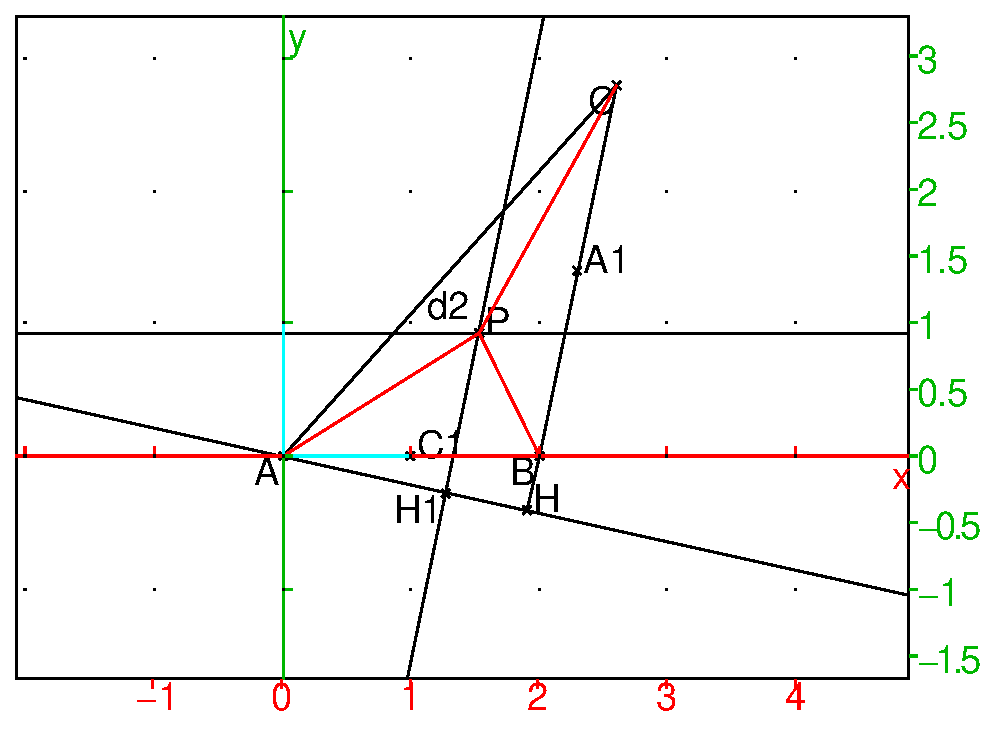
\includegraphics[width=\textwidth]{barycentre}\\
On trouve :
$P$ est le {\tt point(1/3*a+1/3*b+(i)/3*c)},\\
$A1$ est le {\tt point(1/2*a+1/2*b+(i)/2*c)}\\
$C1$ est le {\tt point(1/2*b)}\\
$G$ est le {\tt point((b+a+(i)*c)/3)}\\
Donc \\
$A1$ est le milieu de $BC$ et $C1$ est le milieu de $BC$
$P$ est l'isobarycentre des points $A,B,C$.
\item $P$, le barycentre de $C,1$, $A,2$, $B,3$ r\'epond \`a la question.
\item $P$, le barycentre de $C,n$, $A,p$, $B,q$ r\'epond \`a la question.
\item %partager.xws
{\bf Lemme1}\\
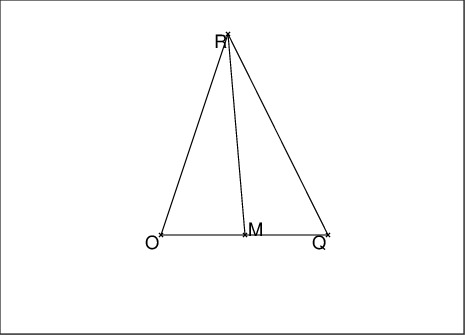
\includegraphics[width=\textwidth]{partager1}\\
Soit un triangle $OQR$ et un point $M$ sur le segment $OQ$ alors
aire de $OMR$=aire de $MQR$ est \'equvalent \`a $M$ est le milieu de $OQ$
{\bf Lemme2}
Soit un quadrilat\`ere  $OPQR$.\\
On note  les parall\`eles $d1$ et $d2$\`a $OQ$  et $h$ la distance entre $d1$ et $d2$, alors :\\
aire($OPQR$)=longueur($OQ$)*$h/2$.
{\bf Lemme3}
Soit un quadrilat\`ere $OPQR$ alors:\\
aire($OPQ$)=aire($OQR$) est \'equivalent \`a $OQ$ passe par le milieu de $PR$.\\
Les d\'emonstrations sont \`evidentes car l'aire d'un triangle est \'egale \`a :
base*hauteur/2.\\
Pour le Lemme1 :\\
$OPR$ (resp $PQR$) ont comme base $OP$ (resp $PQ$) et la m\^eme hauteur.\\
Pour le Lemme2 :\\
\'evident si $OPQR$ est convexe.\\
sinon\\
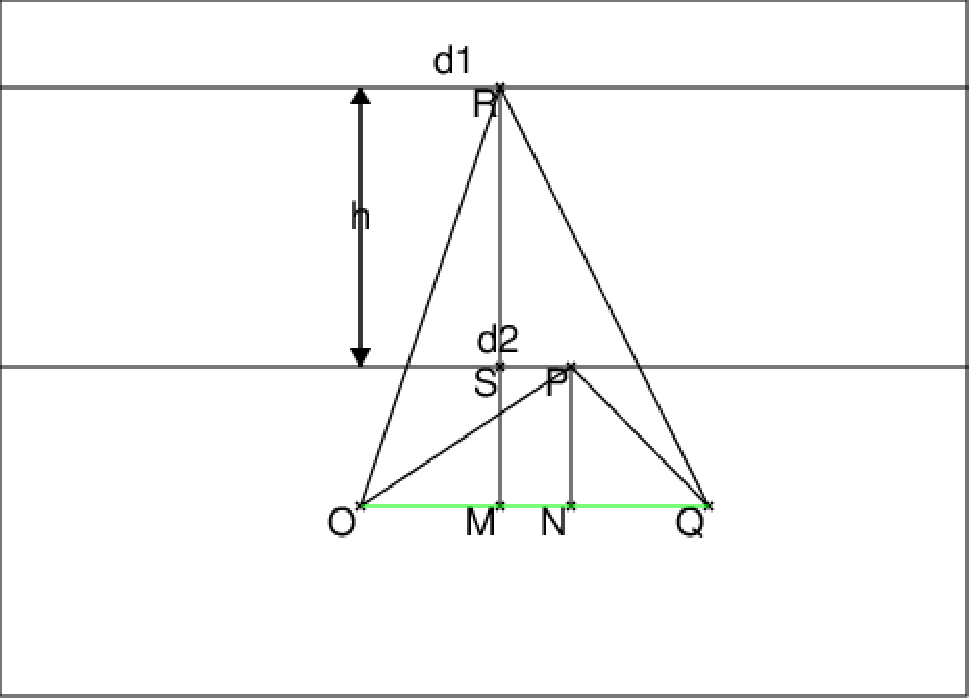
\includegraphics[width=\textwidth]{partager2}\\
aire($OPQR$)=aire($OQR$)-aire($OPQ$)=\\
longueur($OQ$)*(longueur($RM$)-longueur($PN$)/2=longueur($OQ$)*h/2
Pour le Lemme3 :\\
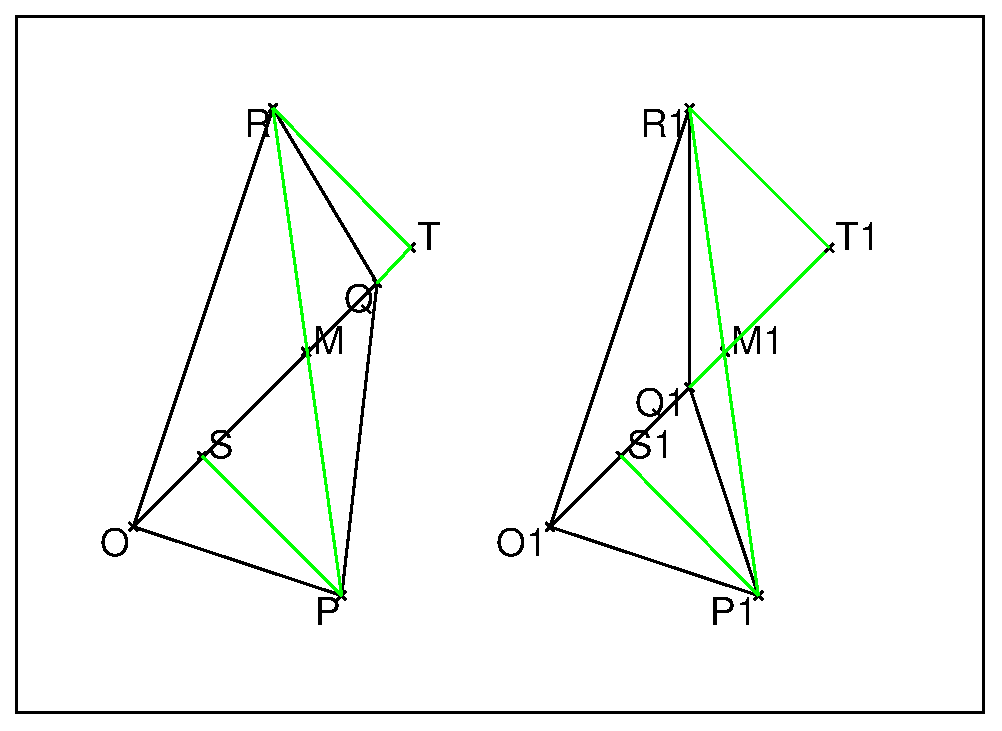
\includegraphics[width=\textwidth]{partager3}\\
$OPQ$ et $OQR$ ont comme base $OQ$ donc \\
aires \'egales est \'equivalent \`a m\^eme hauteur qui est \'equivalent \`a 
$OQ$ passe par le milieu de $PR$.\\
Soit un quadrilat\`ere convexe $ABCD$.\\
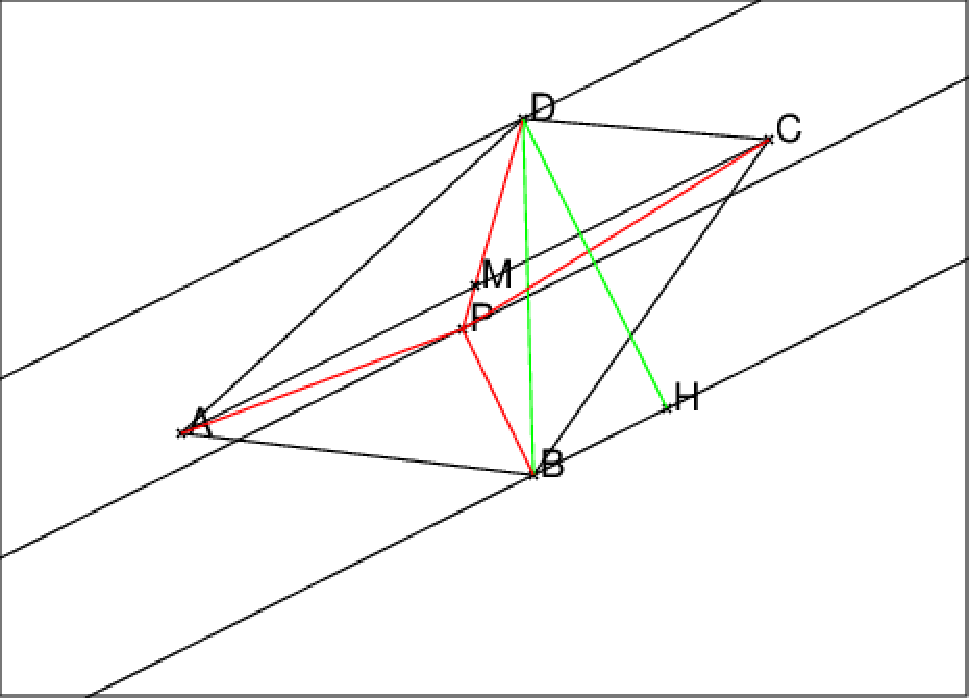
\includegraphics[width=10cm]{partager}\\
On cherche tout d'abord un point $P$ tel que :\\
aire($ABCP$)=aire($APCD$).\\
On m\`ene par $B$ et $D$ les parall\`eles $d1$ et $d2$\`a $AC$.
D'apr\`es le {\tt lemme 2} $P$ se trouve sur la parall\`ele \'equidistante \`a 
$d1$ et $d2$.\\
On veut aussi que :\\
aire($ADP$)=aire($CDP$)\\
La base commune est $DP$, d'apr\`es le {\tt lemme 3}, $DP$ passe par le milieu 
$M$ de $AC$ i.e $D,P,M$ sont align\`'es (c'est vrai sur la figure).\\
aire($ABP$)=aire($CBP$)\\
La base commune est $BP$, d'apr\`es le {\tt lemme 3}, $BP$ passe par le milieu 
$M$ de $AC$ i.e $B,P,M$ sont align\`'es (ce n'est pas vrai sur la figure).\\
Donc, si les 4 aires sont \'egales, on a :
$P$ est en $M$ ou $P$ est diff\'erent de $M$ et donc les points $D,P,M,B$ sont 
align\'es.\\
Si $P$ est en $M$, $P$ se trouve sur $AC$ donc $AC$ est la parall\`ele 
\'equidistante \`a $d1$ et $d2$. Donc $AC$ passe par le milieu de $BD$.\\ 
Si $P$ est diff\'erent de $M$, les points $D,P,M,B$ sont align\'es. Donc
$BD$ passe par le milieu $M$ de $AC$ et $P$ est en $N$ milieu de $BD$
d'apr\`es le {\tt lemme 1}\\
{\tt En r\'esum\'e}
On peut un point $P$ int\'erieur \`a un quadrilat\`ere convexe $ABCD$ qui 
partage ce quadrilat\`ere en 4 triangles de m\^eme aire si et seulement si l'une
des diagonales de $ABCD$ passe par le milieu de l'autre diagonale : $P$ est 
alors le milieu de la diagonale qui passe par le milieu de l'autre diagonale.
\noindent
\begin{minipage}[h]{7cm}
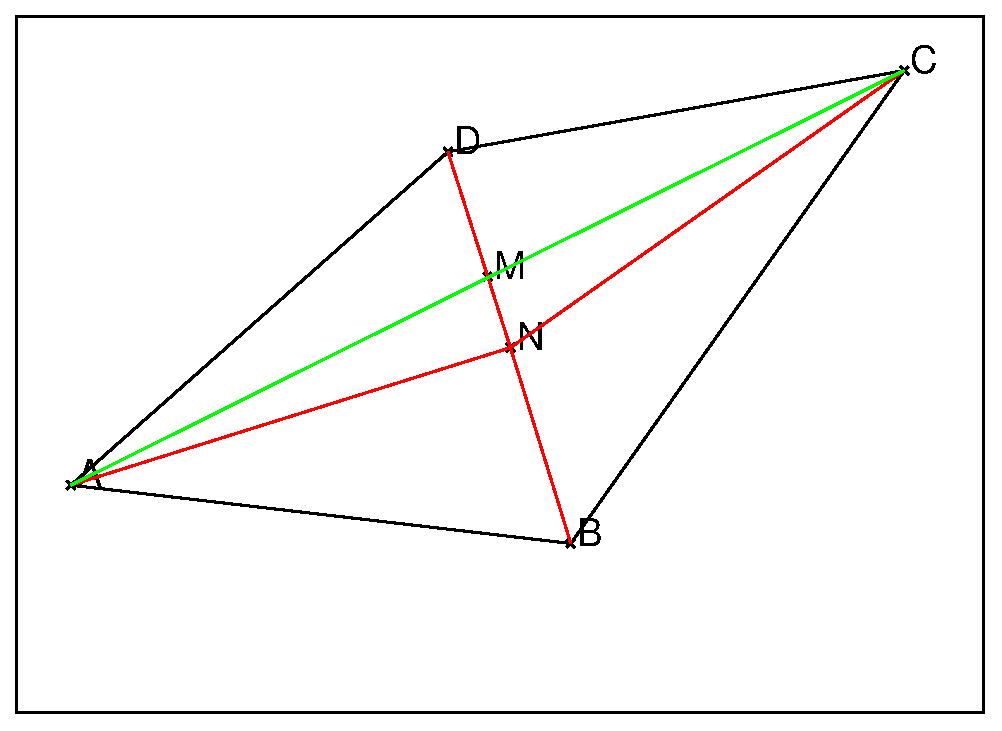
\includegraphics[width=\textwidth]{partager4}
\end{minipage}
\begin{minipage}[h]{7cm}
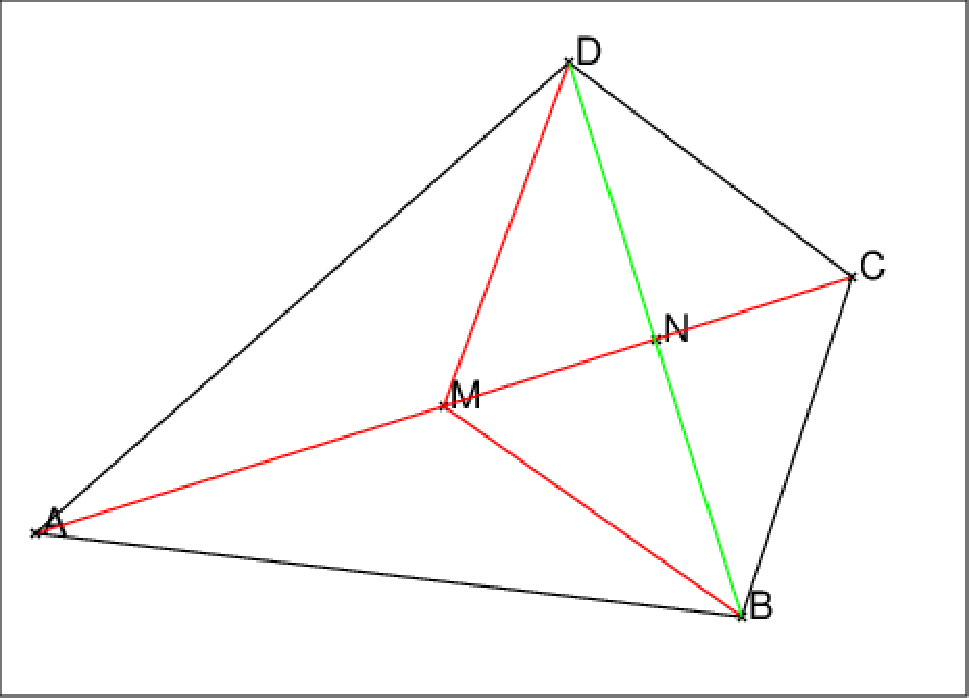
\includegraphics[width=\textwidth]{partager5}
\end{minipage}
\end{itemize}
\subsection{Bissectrice d'un angle}\index{bissectrice}\index{exbissectrice}
\'Etant donn\'e trois points {\tt A}, {\tt B} et {\tt C} les commandes :\\
{\tt bissectrice(A,B,C)} trace la bissectrice int\'erieure de l'angle $A$ du  
triangle $ABC$.\\
{\tt exbissectrice(A,B,C)} trace la bissectrice ext\'erieure de l'angle $A$
 du  triangle $ABC$.\\
{\bf Activit\'e}\\
Cr\'eer un triangle {\tt ABC}.\\
Construire  les bissectrices de l'angle $A$ du  
triangle $ABC$, en utilisant la m\^eme construction qu'avec un compas et en 
utilisant l'instruction {\tt mediatrice}.\\
{\bf R\'eponse}\\
On clique avec la souris pour avoir un triangle {\tt ABC}.\\
On tape :\\
{\tt C1:=cercle(A,2)} trace un cercle de centre {\tt A} et de rayon {\tt 2}.\\
{\tt D:=inter(C1,droite(A,B))} d\'efinit l'intersection du cercle {\tt C1} 
et de la droite $AB$.\\ 
{\tt E:=inter(C1,droite(A,C))} d\'efinit l'intersection du cercle {\tt C1}
et de la droite $AC$.\\
{\tt mediatrice(D[0],E[0])}\\
{\tt mediatrice(D[1],E[0])}\\
%La liste des instructions se trouve dans {\tt geo2} : c\'eer trois points {\tt A, B, C} puis, faire {\tt Charger session} du menu {\tt Fich} de {\tt Xcas} et selectionner {\tt geo2} du r\'ep\'ertoire {\tt examples/geo} pour ex\'ecuter ce fichier.
On peut aussi comme exercice de programmation d\'efinir les fonctions 
{\tt Bissectrice} et {\tt Exbissectrice} (il faut commencer les noms des 
fonctions par une majuscule car {\tt bissectrice} et {\tt exbissectrice} sont 
des commandes de {\tt Xcas}).\\ 
On tape si on a d\'efini  la fonction {\tt Mediatrice} :\\
{\tt Bissectrice(A,B,C):=Mediatrice(inter\_unique(demi\_droite(A,B),\\
cercle(A,2)),inter\_unique(demi\_droite(A,C),cercle(A,2)))}\\
{\tt Exbissectrice(A,B,C):=\{local C1:=A+(A-C);Bissectrice(A,B,C1)\}}\\
\subsection{Report d'une longueur}\index{longueur}
\'Etant donn\'es trois points {\tt A} {\tt B} et {\tt C}, on veut construire un
point {\tt D} pour que  $AD = BC$. \\
On utilise la commande {\tt cercle} et on tape :\\
{\tt D:= element(cercle(A,B-C))}\\
L'instruction {\tt longueur(B,C)} renvoie la longueur du segment $BC$ (les 
unit\'es \'etant d\'efinies par le choix de {\tt WX-, WX+} et de 
{\tt WY-, WY+}) effectu\'e dans la fen\^etre d'initialisation graphique.\\
Si l'on veut reporter une longueur dans une direction donn\'ee, on multiplie
cette longueur par le vecteur unitaire de cette direction.\\
{\bf Exemple} :\\
\'Etant donn\'es trois points {\tt A} {\tt B} et {\tt C}, construire sur la 
demi-droite $AB$, un point $D$ tel que $AD=AC$.\\
On tape :\\
{\tt D:=A+longueur(A,C)*(B-A)/longueur(A,B)}\\
ou encore \\
{\tt D:=inter\_unique(cercle(A,C-A),demi\_droite(A,B))}

\subsection{Report d'un angle}\index{angle}\index{radian}\index{degree}
\'Etant donn\'es deux points {\tt A} et {\tt B}, on veut construire {\tt C} 
pour que l'angle 
 $(\overrightarrow {AB},\overrightarrow {AC})$ soit de mesure donn\'ee
par exemple 72 degr\'es ou $2*\pi/5$ radians.\\
On tape, si on a coch\'e {\tt radian} dans la fen\^etre de configuration du 
{\tt CAS} :\\
{\tt D:=rotation(A,2*pi/5,droite(A,B))}\\
ou, si on est en degr\'e (on n'a pas coch\'e {\tt radian}) :\\
{\tt D:=rotation(A,72,droite(A,B))}\\
puis on tape :\\
{\tt C:=element(D)} \\
L'instruction {\tt angle(A,B,C)} donne la mesure en radians (ou en degr\'es) 
de l'angle
 $(\overrightarrow {AB},\overrightarrow {AC})$, on peut donc v\'erifier la 
construction demand\'ee.  \\
\'Etant donn\'e deux points {\tt A} et {\tt B}, on veut construire {\tt C} 
pour que l'angle 
 $(\overrightarrow {AB},\overrightarrow {AC})$ soit \'egal \`a l'angle 
$(\overrightarrow {OM},\overrightarrow {OP})$.\\
On tape :\\
{\tt D:=rotation(A,angle(O,M,P), droite(A,B));}\\
{\tt C:=element(D)}

\subsection{Perpendiculaire \`a la droite $D$ passant par $A$}\index{perpendiculaire}
\'Etant donn\'e trois points {\tt A} {\tt B} et {\tt C}, on veut construire 
la perpendiculaire, passant par A, \`a la droite BC.\\
On tape :\\
{\tt perpendiculaire(A,droite(B,C))} ou,\\
{\tt hauteur(A,B,C)} (voir aussi \ref{sec:droitetri}) ou,\\
on utilise le nombre complexe {\tt i} : {\tt droite(A,A+i*(C-B))}.\\
{\bf Activit\'e}\\
Cr\'eer un point {\tt A} et une droite {\tt BC} ne passant pas par {\tt A}.\\
Construire  la perpendiculaire \`a la droite $BC$ passant par $A$, en utilisant
la m\^eme construction qu'avec un compas.\\
{\bf R\'eponse}\\
On clique avec la souris pour avoir un point {\tt A} et deux points {\tt B} et
 {\tt C} et le segment {\tt BC}.\\
On tape :\\
{\tt C1:=cercle(B,A-B)} trace le cercle de centre $B$ passant par $A$\\
{\tt C2:=cercle(C,A-C)} trace le cercle de centre $C$ passant par $A$\\
{\tt droite(inter(C1,C2))} trace la droite qui joint les points d'intersection
des deux cercles pr\'ec\'edents.\\
%La liste des instructions se trouve dans {\tt geo3}  : c\'eer trois points {\tt A, B, C}, puis  faire {\tt Charger session} du menu {\tt Fich} de {\tt Xcas} et selectionner {\tt geo3} du r\'ep\'ertoire {\tt examples/geo} pour ex\'ecuter ce fichier.\\
{\bf Activit\'e}\\
Cr\'eer un segment {\tt AB}.\\
Construire  la perpendiculaire \`a la droite $AB$ passant par $A$ en utilisant 
la m\^eme construction qu'avec un compas.\\
{\bf R\'eponse}\\
On clique avec la souris pour avoir deux points {\tt A} et {\tt B} et le 
segment {\tt AB}.\\
On tape :\\
{\tt C3:=cercle(A,B-A)} trace le cercle de centre $A$ passant par $B$\\
{\tt mediatrice(inter(C3,droite(A,B)))} 
trace la mediatrice des deux points d\'efinit par {\tt inter(C3,droite(A,B))},
cette m\'ediatrice passe par $A$ et est perpendiculaire \`a $AB$.\\
%La liste des instructions se trouve dans {\tt geo4}  : cr\'eer deux points 
%{\tt A, B}, puis  faire {\tt Charger session} du 
%menu {\tt Fich} de {\tt Xcas} et selectionner {\tt geo4} du r\'ep\'ertoire 
%{\tt examples/geo} pour ex\'ecuter ce fichier.
On peut aussi comme exercice de programmation d\'efinir la fonction 
{\tt Perpendiculaire} (il faut commencer le nom de la fonction par une 
majuscule car {\tt perpendiculaire} est une commande de {\tt Xcas}).\\ 
On tape ({\tt A} est un point et {\tt d} est une droite) :
\begin{verbatim}
Perpendiculaire(A,d):={
local L,M,E:=element(d);
si est_element(A,d) alors 
  L:=inter(d,cercle(A,1)); 
  retourne simplify(affixe(A)),simplify(equation(mediatrice(L))); 
fsi;  
si angle(E,d,A)==pi/2 or angle(E,d,A)==-pi/2  alors 
  retourne simplify(affixe(E)),equation(droite(A,E)); 
fsi;
M:=milieu(op(inter(d,cercle(A,E-A))));
retourne simplify(affixe(M)),equation(droite(A,M));
}:;
\end{verbatim}
ainsi {\tt Perpendiculaire} renvoie l'affixe de la projection orthogonale 
{\tt E} de {\tt A} sur {\tt d} et l'\'equation de la droite {\tt A,E}.\\
On tape :\\
{\tt Perpendiculaire(point(1),droite(0,1+i))}\\
On obtient :\\
{\tt i/2+1/2,y=(-x+1)}\\
On tape :\\
{\tt Perpendiculaire(point(1),droite(-2,1+i))}\\
On obtient :\\
{\tt i/2-1/2,y=(-3*x+3)}
\subsection{Parall\`ele \`a une droite passant par A}\index{parallele}
\'Etant donn\'e trois points {\tt A} {\tt B} et {\tt C}, on veut construire 
la parall\`ele \`a la droite BC passant par A.\\
On tape :\\
{\tt parallele(A,droite(B,C))}\\
{\bf Activit\'e}\\
Cr\'eer un point {\tt A} et un segment {\tt BC} ne passant pas par {\tt A}.
Construire la parall\`ele \`a la droite $BC$ passant par $A$ en utilisant 
l'instruction {\tt perpendiculaire}.\\
{\bf R\'eponse}\\
On clique avec la souris pour avoir un point {\tt A} et deux points {\tt B} et
 {\tt C} et le segment {\tt BC}.\\
On tape :\\
{\tt D:=perpendiculaire(A,droite(B,C))}\\
cela trace la perpendiculaire \`a $BC$ passant par $A$\\
{\tt P:=perpendiculaire(A,D)}\\
cela trace la perpendiculaire \`a $D$ passant par $A$.\\
La liste des instructions se trouve dans {\tt geo5}  : cr\'eer trois points 
{\tt A, B, C}, puis  faire {\tt Charger session} du 
menu {\tt Fich} de {\tt Xcas} et selectionner {\tt geo5} du r\'ep\'ertoire 
{\tt examples/geo} pour ex\'ecuter ce fichier.\\

On peut, comme exercice de programmation d\'efinir la fonction 
{\tt Parallele} (il faut commencer le nom de la fonction par une majuscule car 
{\tt parallele} est une commande de {\tt Xcas}).\\ 
On tape ({\tt A} est un point et {\tt d} est une droite) :
\begin{verbatim}
Parallele(A,d):={
local d1:=droite(Perpendiculaire(A,d)[1]);
Perpendiculaire(A,d1)[1];
}:;
\end{verbatim}
{\tt Parallele} renvoie l'\'equation de la parall\`ele \`a {\tt d} passant par
{\tt A}.\\
On tape :\\
{\tt Parallele(point(i),droite(0,1+i))}\\
On obtient :\\
{\tt y=(x+1)}
 \subsection{Parall\`eles \`a une droite situ\'ees \`a une distance $d$ de cette droite}
{\bf Activit\'e}\\
Cr\'eer un point {\tt A} et un segment {\tt BC} ne passant pas par {\tt A}.\\
Puis cr\'eer un point {\tt D} pour d\'efinir $d=${\tt longueur(A,D)}. \\
Construire les parall\`eles \`a la droite $BC$ situ\'ees \`a une distance 
$d=${\tt longueur(A,D)} de $BC$.\\
{\bf R\'eponse}\\
On clique avec la souris pour avoir un point {\tt A} et deux points {\tt B} et
 {\tt C} et le segment {\tt BC}, puis on clique avec la souris pour avoir un 
point {\tt D} ($d=longueur(A,D)$).\\
On tape :\\
{\tt D1:=perpendiculaire(B,droite(B,C));}\\
{\tt C1:=cercle(B,longueur(A,D));}\\
{\tt I:=inter(D1,C1);}\\
{\tt E:=I[0];}\\
{\tt F:=I[1];}\\
ou on utilise les nombres complexes pour d\'efinir {\tt E} et {\tt F} :\\
{\tt E:=B+i*(C-B)*longueur(A,D)/longueur(B,C)} le point {\tt E} est \`a une 
distance $d=longueur(A,D)$ de la droite $BC$,\\
{\tt F:=B-i*(C-B)*longueur(A,D)/longueur(B,C)} le point {\tt F} est \`a une 
distance $d=longueur(A,D)$ de la droite $BC$ ({\tt E} et {\tt F} sont 
sym\`etriques par rapport \`a $BC$),\\
puis,\\
{\tt parallele(E,droite(B,C))} trace une parall\`ele \`a la droite $BC$ situ\'ees \`a une distance $d=longueur(A,D)$ de $BC$.\\
{\tt parallele(F,droite(B,C))} trace l'autre parall\`ele \`a la droite $BC$ situ\'ees \`a une distance $d=longueur(A,D)$ de $BC$.\\
%La liste des instructions se trouve dans {\tt geo6} : cr\'eer trois points 
%{\tt A, B, C}, puis  faire {\tt Charger session} du 
%menu {\tt Fich} de {\tt Xcas} et selectionner {\tt geo6} du r\'ep\'ertoire 
%{\tt examples/geo} pour ex\'ecuter ce fichier.
\subsection{Tangentes \`a un cercle}\index{tangent}
\'Etant donn\'e un point {\tt A} et un cercle {\tt C}, la commande :\\
{\tt tangent(C,A)} dessine les deux tangentes \`a {\tt C} passant par {\tt A}
si le point {\tt A} est ext\'erieur au cercle.\\
Si le point {\tt A} est ext\'erieur au cercle, {\tt tangent(C,A)} est une liste
 de deux droites (les deux tangentes \`a {\tt C} passant par {\tt A}) et \\
si le point {\tt A} est sur le cercle {\tt tangent(C,A)} est une droite (la
 tangente \`a {\tt C} passant par {\tt A}).\\
{\bf Activit\'e}\\
Tracer les tangentes \`a un cercle passant par un point.\\
Cette activit\'e doit se faire sans utiliser la commande {\tt tangent}.\\
Cr\'eer deux points  {\tt A} et {\tt B}.\\
Cr\'eer un cercle {\tt C1} de centre {\tt A} et passant par {\tt B}.\\
Construire  la tangente au cercle {\tt C1} passant par {\tt B}.\\
 Cr\'eer un point {\tt C} ext\'erieur au cercle  {\tt C1} et construire  les
 tangentes au cercle {\tt C1} passant par {\tt C}.\\
{\bf R\'eponse}\\
On clique avec la souris pour avoir trois points {\tt A}, {\tt B} et {\tt C} 
puis on ex\'ecute la liste des instructions qui se trouve dans {\tt geo7} 
(faire {\tt Charger session} du 
menu {\tt Fich} de {\tt Xcas} et selectionner {\tt geo7} du r\'ep\'ertoire 
{\tt examples/geo} pour ex\'ecuter ce fichier).\\
Voici le d\'etail de {\tt geo7} :\\
{\tt C1:=cercle(A,B-A)} ($C1$ est le cercle de centre $A$ qui passe par $B$),\\
{\tt perpendiculaire(B,droite(A,B))} (on dessine la tangente \`a $C1$ au point $B$),\\
{\tt C2:=cercle(C,A)} ($C2$ est le cercle de diam\`etre $AC$),\\
{\tt E:=inter(C1,C2)} ($E$ d\'esigne les 2 points d'intersection de $C1$ et de $C2$),\\
{\tt droite(E[0],C)} (c'est une tangente \`a $C1$ passant par $C$),\\
{\tt droite(E[1],C)} c'est l'autre tangente \`a $C1$ passant par $C$,\\
{\bf Activit\'e}\\
Tracer un cercle tangent \`a une droite donn\'ee en un point donn\'e et passant
 par un autre point.\\
Cr\'eer trois  points {\tt A}, {\tt B} et {\tt C}.\\
Tracer la droite {\tt D} passant par {\tt A} et {\tt B}.\\
Construire un cercle {\tt C1} passant par {\tt C} et tangent \`a {\tt D} en 
{\tt A}.\\
{\bf R\'eponse}\\
On clique avec la souris pour avoir trois points {\tt A}, {\tt B} et {\tt C} 
puis on ex\'ecute la liste des instructions qui se trouve dans {\tt geo8} 
(faire {\tt Charger session} du 
menu {\tt Fich} de {\tt Xcas} et selectionner {\tt geo8} du r\'ep\'ertoire 
{\tt examples/geo} pour ex\'ecuter ce fichier).\\
Voici le d\'etail de {\tt geo8} :\\
{\tt D:=droite(A,B)} (trace la droite $D$ passant par $A$ et $B$),\\
{\tt P:=perpendiculaire(A,D)} (trace la perpendiculaire \`a  $D$ passant par $A$),\\ 
{\tt M:=mediatrice(A,C)} (trace la m\'ediatrice de $AC$),\\
{\tt N:=inter(P,M)[0]} ($N$ est le point d'intersection des deux droites 
pr\'ec\'edentes),\\
{\tt C1:=cercle(N,A-N)} (trace le cercle de centre $N$ passant par $A$).\\
{\tt C1} repond \`a la question. 
\subsection{Tangentes communes \`a 2 cercles}
Soient {\tt C1:=cercle(A,r1)} et {\tt C2:=cercle(B,r2)}.
Supposons {\tt r1!=r2} alors :\\
 \begin{itemize}
\item si {\tt longueur(A,B)<|r2-r1|} il n'y a pas de tangente commune.
\item si {\tt longueur(A,B)=|r2-r1|} les 2 cercles sont tangents en {\tt C} et 
il y a 1 tangente commune passant par {\tt C} et perpendiculaire \`a {\tt AB}.
\item si {\tt |r2-r1|<longueur(A,B)<r2+r1} il y a 2 tangentes communes 
ext\'erieures qui se coupent en {\tt C} ({\tt CA/CB=r1/r2}).
\item si {\tt longueur(A,B)=r2+r1} les 2 cercles sont tangents en {\tt D} et 
il y a 1 tangente commune passant par {\tt D} et perpendiculaire \`a {\tt AB}
et 2 tangentes communes qui se coupent en {\tt C} ({\tt CA/CB=r1/r2} et
{\tt DA=r1, DB=r2}).
\item si {\tt r2+r1<longueur(A,B)} il y a 2 tangentes communes ext\'erieures
qui se coupent en {\tt C} et 2 tangentes communes int\'erieures
qui se coupent en {\tt D} ({\tt CA/CB=r1/r2} et {\tt DA/DB=r1/r2} avec {\tt D}
entre {\tt A} et {\tt B}).
\end{itemize}
Si {\tt r1=r2} et {\tt A!=B} il y a 2, 3, 4  tangentes communes et si
{\tt r1=r2} et {\tt A=B} une infinit\'e de tangentes communes
Voici le programme g\'en\'eral :
\begin{verbatim}
tangentes(A,r1,B,r2):={
local C1,C2,C,D,p,L,t1,t2;
C1:=cercle(A,r1);
C2:=cercle(B,r2);
si r1==0 alors
return tangente(C2,A);
fsi;
si r2==0 alors
return tangente(C1,B);
fsi;
si longueur2(A,B)<(r2-r1)^2 alors
return [];
fsi;
si r1==r2 alors
si A==B alors return [infinity]; fsi; 
p:=perpendiculaire(B,droite(A,B));
L:=inter(C2,p);
t1:=parallele(L[0],droite(A,B));
t2:=parallele(L[1],droite(A,B)); 
si longueur2(A,B)<(r2+r1)^2 alors 
return [t1,t2];
sinon 
return concat([t1,t2],tangente(C1,milieu(A,B)));
fsi;
fsi;
C:=division_point(A,B,r1/r2);
si longueur2(A,B)<(r2+r1)^2 alors
return tangente(C1,C);
sinon
D:=division_point(A,B,-r1/r2);
return concat(tangente(C1,C),tangente(C1,D));
fsi;
}:;
\end{verbatim}
{\bf Activit\'e}
Tracer les tangentes ext\'erieures communes \`a deux cercles s\'ecants ou 
ext\'erieurs avec une construction g\'eom\'etrique niveau 3i\`eme sans utiliser
la primitive {\tt tangente}.\\
On suppose que si {\tt C1:=cercle(A,r1)} et {\tt C2:=cercle(B,r2)} alors :\\
{\tt longueur(A,B)>=|r2-r1|}.
\begin{itemize}
\item Si les 2 cercles ont des rayons \'egaux, la solution est facile car les 
tangentes ext\'erieures communes sont parall\`eles \`a la droite des centres et
les points de contact sont sur les perpendiculaires  \`a la droite des 
centres passant respectivement par les centres.\\
On tape :
\begin{verbatim}
A:=point([-3.5,0.5],affichage=4);
c1:=cercle(A,4,affichage=4);
B:=point([1.3,1.4],affichage=4);
c2:=cercle(B,4,affichage=4);
p:=perpendiculaire(B,droite(A,B),affichage=ligne_tiret_point);
L:=inter(c2,p);
t1:=parallele(L[0],droite(A,B),affichage=1);
t2:=parallele(L[1],droite(A,B),affichage=1);
\end{verbatim}
On obtient :\\
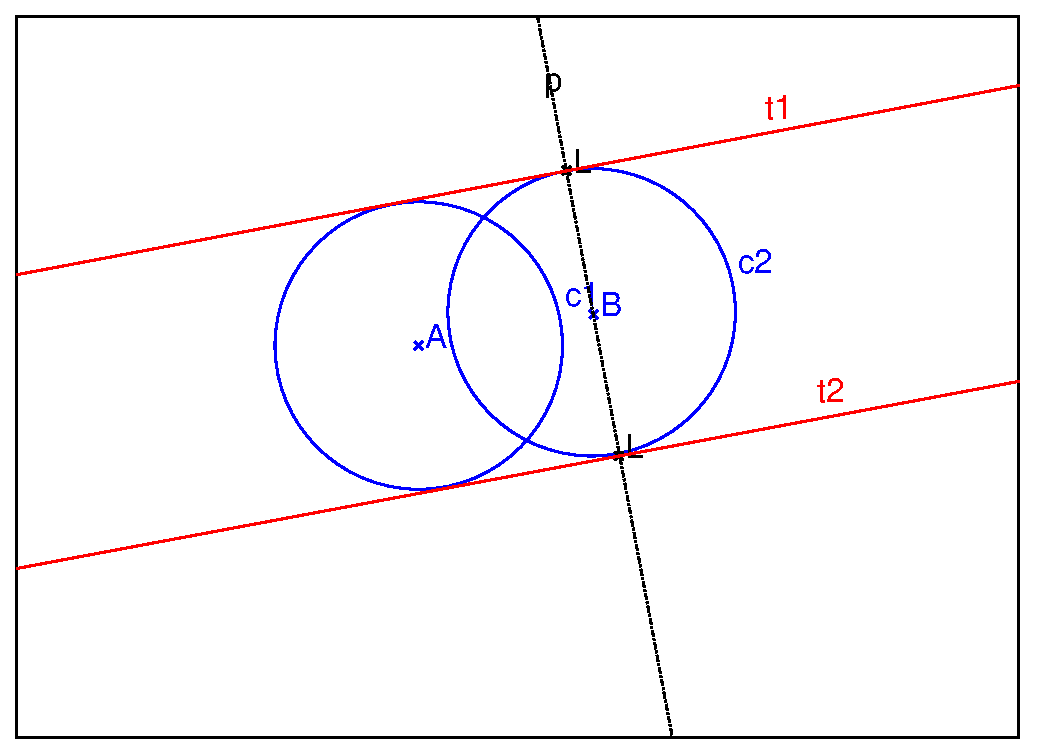
\includegraphics[width=12cm]{tangent2C0}
\item Si les 2 cercles ont des rayons diff\'erents, par exemple si :\\
{\tt C1:=cercle(A,r1)} et {\tt C2:=cercle(B,r2)} avec {\tt r1<r2}.\\
Si {\tt K1} et {\tt K2} sont les points de contact d'une tangente ext\'erieure 
commune \`a {\tt C1} et {\tt C2}, le quadrilat\`ere $A,B,K2,K1$ est un trap\`eze
rectangle que l'on peut partager en un rectangle $A,R,K2,K1$ et un triangle 
rectangle $A,B,R$.\\
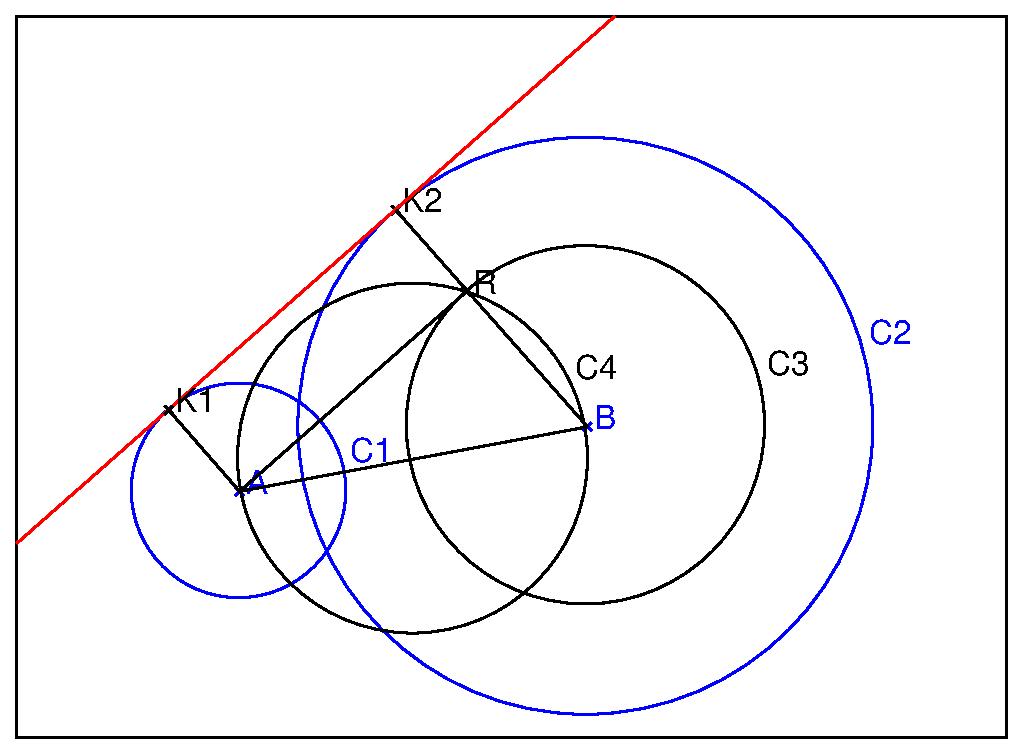
\includegraphics[width=\textwidth]{tangented}\\
Donc $R$ se trouve sur le cercle de diam\`etre $AB$ et sur le cercle de centre $B$ et de rayon $r2-r1$. \\
On tape :
\begin{verbatim}
A:=point([-3.5,0.5],affichage=4);
r1:=1.5;
C1:=cercle(A,r1,affichage=4);
B:=point([1.3,1.4],affichage=4);
r2:=4;
C2:=cercle(B,r2,affichage=4);
C3:=cercle(B,r2-r1);
C4:=cercle(A,B);
L:=inter(C3,C4);
T1:=inter_unique(demi_droite(B,L[0]),C2);
T2:=inter_unique(demi_droite(B,L[1]),C2);
t1:=parallele(T1,droite(A,L[0]),affichage=1);
t2:=parallele(T2,droite(A,L[1]),affichage=1);
segment(B,T1,affichage=ligne_tiret_point);
segment(B,T2,affichage=ligne_tiret_point);
segment(A,B);
\end{verbatim}
On obtient :\\

\includegraphics[width=\textwidth]{tangent2c}
\item Avec un programme :\\
Si {\tt C1:=cercle(A,r1)} et {\tt C2:=cercle(B,r2)} alors on doit avoir :\\
{\tt longueur2(A,B)>=(r2-r1)\verb|^|2}.\\
On tape dans l'\'editeur de programmes :
\begin{verbatim}
tangente2c(A,r1,B,r2):={
local C1,C2,C3,C4,L,T1,T2,t1,t2,r,C,p;
si r1>r2 alors 
r:=r1;r1:=r2;r2:=r;
C:=A;A:=B;B:=C;
fsi;
C1:=cercle(A,r1);
C2:=cercle(B,r2);
si longueur2(A,B)<(r2-r1)^2 alors
return [C1,C2];
fsi;
si r1==r2 alors 
p:=perpendiculaire(B,droite(A,B));
L:=inter(C2,p);
t1:=parallele(L[0],droite(A,B),affichage=1);
t2:=parallele(L[1],droite(A,B),affichage=1); 
return [C1,C2,t1,t2];
fsi;
C3:=cercle(B,r2-r1);
C4:=cercle(A,B);
L:=inter(C3,C4);
T1:=inter_unique(demi_droite(B,L[0]),C2);
T2:=inter_unique(demi_droite(B,L[1]),C2);
t1:=parallele(T1,droite(A,L[0]),affichage=1);
t2:=parallele(T2,droite(A,L[1]),affichage=1);
return [C1,C2,t1,t2]
}:;
\end{verbatim}
\end{itemize}

{\bf Activit\'e}
Tracer les tangentes int\'erieures communes \`a deux cercles  ext\'erieurs.\\
Si les 2 cercles sont ext\'erieurs, par exemple si :\\
{\tt C1:=cercle(A,r1)} et {\tt C2:=cercle(B,r2)}, on doit avoir {\tt AB>r1+r2}.\\
Si {\tt K1} et {\tt K2} sont les points de contact d'une tangente int\'erieure 
commune \`a {\tt C1} et {\tt C2}, la parall\`ele \`a $K1K2$ men\'ee par $A$
coupe $BK2$ en $R$. On a $BR=r2+r1$ et le triangle $A,B,R$ est rectangle en $R$.\\
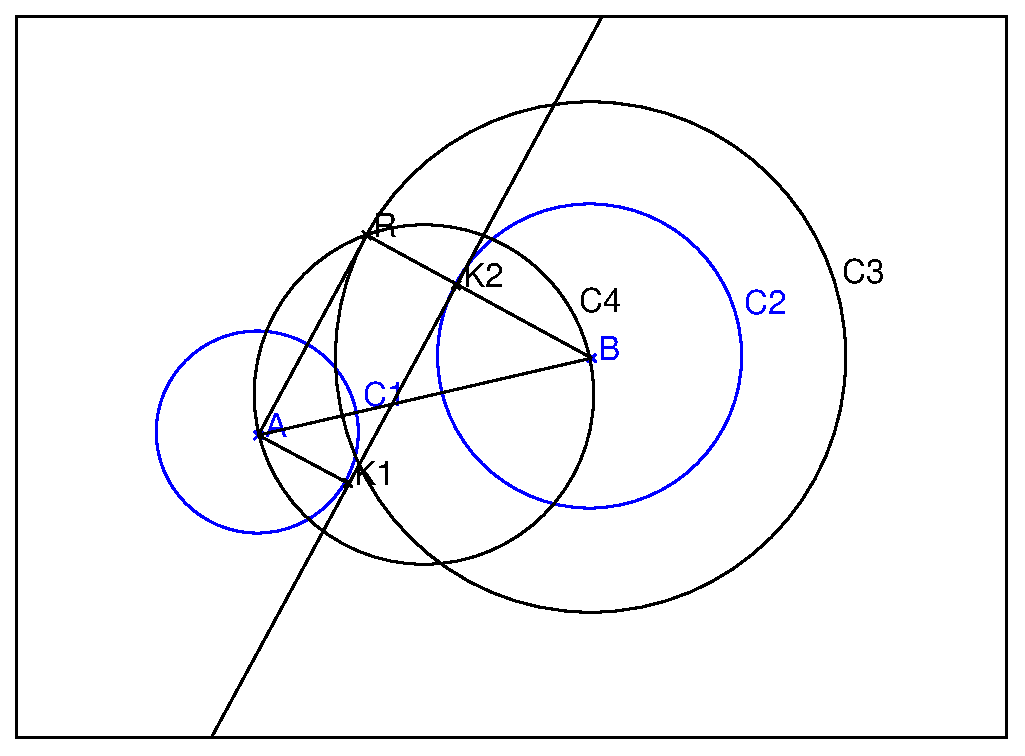
\includegraphics[width=\textwidth]{tangentid}\\
Donc $R$ se trouve sur le cercle de diam\`etre $AB$ et sur le cercle de centre $B$ et de rayon $r2-r1$.\\
\begin{itemize}
\item On tape dans un niveau de g\'eom\'etrie 2D :
\begin{verbatim}
A:=point([-3.5,0.5],affichage=4);
r1:=1.5;
C1:=cercle(A,r1,affichage=4);
B:=point([3,2],affichage=4);
r2:=4;
C2:=cercle(B,r2,affichage=4);
C3:=cercle(B,r2+r1);
C4:=cercle(A,B);
L:=inter(C3,C4);
T1:=inter_unique(demi_droite(B,L[0]),C2);
T2:=inter_unique(demi_droite(B,L[1]),C2);
t1:=parallele(T1,droite(A,L[0]),affichage=1);
t2:=parallele(T2,droite(A,L[1]),affichage=1);
segment(B,L[0],affichage=ligne_tiret_point);
segment(B,L[1],affichage=ligne_tiret_point);
segment(A,B);
\end{verbatim}
On obtient :\\

\includegraphics[width=\textwidth]{tangent2c2}
\item Avec un programme :\\
Si {\tt C1:=cercle(A,r1)} et {\tt C2:=cercle(B,r2)} alors on doit avoir :\\
{\tt longueur2(A,B)>=(r2-r1)\verb|^|2}.\\
On tape dans l'\'editeur de programmes :
\begin{verbatim}
tangenti2c(A,r1,B,r2):={
local C1,C2,C3,C4,L,T1,T2,t1,t2,r,C,p;
si r1>r2 alors 
r:=r1;r1:=r2;r2:=r;
C:=A;A:=B;B:=C;
fsi;
C1:=cercle(A,r1);
C2:=cercle(B,r2);
si longueur2(A,B)<(r2+r1)^2 alors
return [C1,C2];
fsi;
si longueur2(A,B)<(r2+r1)^2 alors
return [C1,C2];
fsi;
C3:=cercle(B,r2+r1);
C4:=cercle(A,B);
L:=inter(C3,C4);
T1:=inter_unique(demi_droite(B,L[0]),C2);
T2:=inter_unique(demi_droite(B,L[1]),C2);
t1:=parallele(T1,droite(A,L[0]),affichage=1);
t2:=parallele(T2,droite(A,L[1]),affichage=1);
return [C1,C2,t1,t2]
}:;
\end{verbatim}
\end{itemize}
Voici le programme g\'en\'eral :
\begin{verbatim}
tangentei2c(A,r1,B,r2):={
local C1,C2,C3,C4,C5,L,L1,T1,T2,T3,T4,t1,t2,t3,t4,r,C,p;
si r1>r2 alors 
r:=r1;r1:=r2;r2:=r;
C:=A;A:=B;B:=C;
fsi;
C1:=cercle(A,r1);
C2:=cercle(B,r2);
si longueur2(A,B)<(r2-r1)^2 alors
return [C1,C2];
fsi;
C4:=cercle(A,B);
si longueur2(A,B)>=(r2+r1)^2 alors
C5:=cercle(B,r2+r1);
L1:=inter(C5,C4);
T3:=inter_unique(demi_droite(B,L1[0]),C2);
T4:=inter_unique(demi_droite(B,L1[1]),C2);
t3:=parallele(T3,droite(A,L1[0]),affichage=1);
t4:=parallele(T4,droite(A,L1[1]),affichage=1);
fsi;
si r1==r2 alors
si A==B alors return [C1,C2,infinity]; fsi; 
p:=perpendiculaire(B,droite(A,B));
L:=inter(C2,p);
t1:=parallele(L[0],droite(A,B),affichage=1);
t2:=parallele(L[1],droite(A,B),affichage=1); 
si longueur2(A,B)<(r2+r1)^2 alors 
return [C1,C2,t1,t2];
sinon return [C1,C2,t1,t2,t3,t4];
fsi;
fsi;
C3:=cercle(B,r2-r1);
L:=inter(C3,C4);
T1:=inter_unique(demi_droite(B,L[0]),C2);
T2:=inter_unique(demi_droite(B,L[1]),C2);
t1:=parallele(T1,droite(A,L[0]),affichage=1);
t2:=parallele(T2,droite(A,L[1]),affichage=1);
si longueur2(A,B)<(r2+r1)^2 alors
return [C1,C2,t1,t2]
sinon return [C1,C2,t1,t2,t3,t4];
fsi;

return [C1,C2,t1,t2,t3,t4];
}:;

\end{verbatim}
On tape :\\
{\tt tangentei2c(point(0,0),1,point(-4,0),2);}\\
On obtient :\\


\includegraphics[width=\textwidth]{tangente4}\\
On tape :\\
{\tt tangentei2c(point(0,0),1,point(-3,0),2);}\\
On obtient :\\

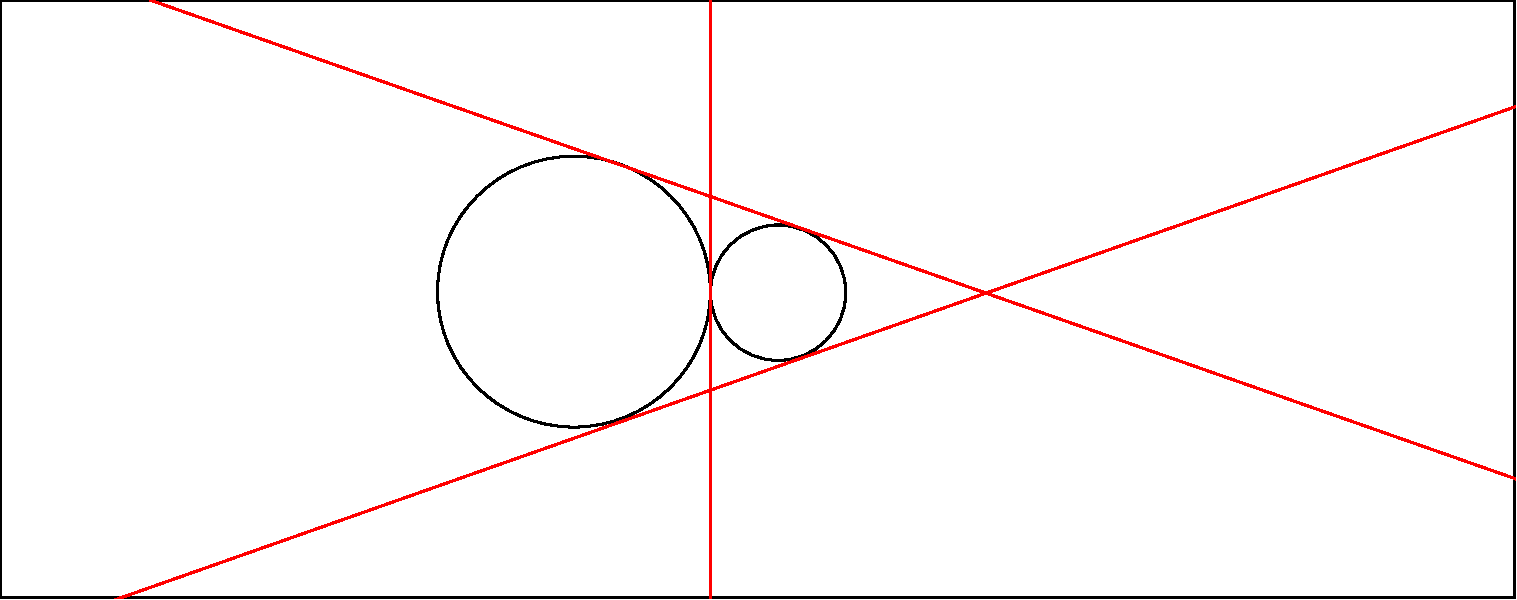
\includegraphics[width=\textwidth]{tangente3}\\
On tape :\\
{\tt tangentei2c(point(0,0),1,point(-2,0),2);}\\
On obtient :\\

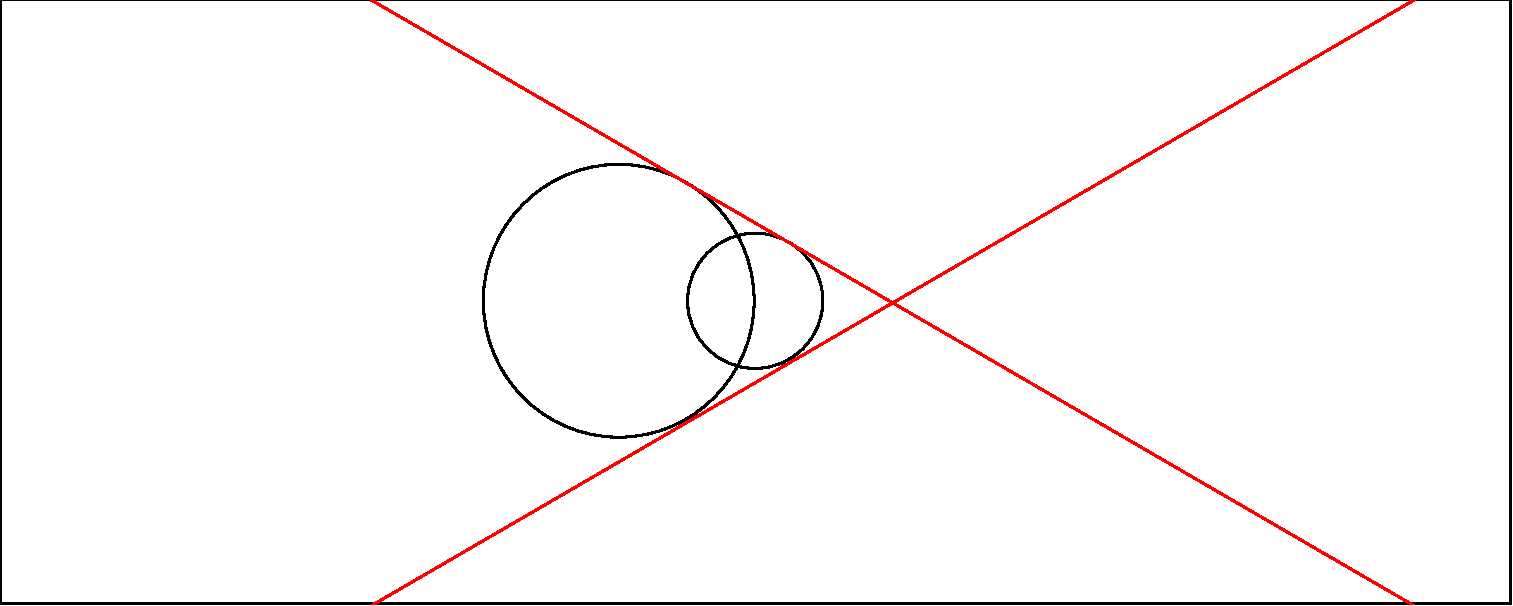
\includegraphics[width=\textwidth]{tangente2}\\
On tape :\\
{\tt tangentei2c(point(0,0),1,point(-1,0),2)}\\
On obtient :\\


\includegraphics[width=\textwidth]{tangente1}\\
On tape :\\
{\tt tangentei2c(point(0,0),1,point(-0.5,0),2)}\\
On obtient :\\

\includegraphics[width=\textwidth]{tangente0}

\section{Une construction plus difficile}
Soit un rectangle $ABCD$ tel que $AB=a$ et $AD=b$.\\
On cherche les conditions que doivent v\'erifier $x$ et $y$ pour que l'on puisse
construire un point $M$, de coordonn\`ees $(x,y)$, \`a l'int\'erieur du 
rectangle v\'erifiant :\\
$MD=3$, $MC=4$ et $MB=5$.\\ 
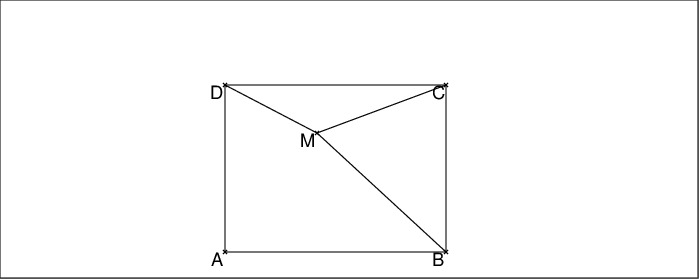
\includegraphics[width=\textwidth]{rect345}\\
Si l'affixe de $M$ est $m+i*n$, \'ecrire les relations qui lient $m,n,a,b$.\\
Faire la construction avec {\tt Xcas}.\\

On a donc :\\
$0\leq m\leq 3$ et $0\leq n\leq 5$\\
On pose :\\
{\tt M:=point(m+i*n)}\\
{\tt A:=point(0)}\\
{\tt B:=point(a)}\\
{\tt C:=point(a+i*b)}\\
{\tt D:=point(i*b)}\\
On tape :\\
{\tt longueur2(M,D)-9}\\
On obtient :\\
{\tt (m)\verb|^|2+(-b+n)\verb|^|2-9}\\
On tape :\\
{\tt longueur2(M,C)-16}\\
On obtient :\\
{\tt (-a+m)\verb|^|2+(-b+n)\verb|^|2-16}\\
On tape :\\
{\tt longueur2(M,B)-25}\\
On obtient :\\
{\tt n\verb|^|2+(-a+m)\verb|^|2-25}\\
Donc $m,n,a,b$ v\'erifient les \'equations :\\
$[(m)^2+(-b+n)^2=9,(-a+m)^2+(-b+n)^2=16,n^2+(-a+m)^2=25]$\\
Donc :\\
$m^2+n^2=(m)^2+(-b+n)^2-((-a+m)^2+(-b+n)^2)+n^2+(-a+m)^2=9-16+25=18$\\
Le point $M$ se trouve donc sur le cercle $c$ de centre $A$ et de rayon 
$\sqrt{18}$.\
Comme $0\leq m\leq 3$ et que le point d'affixe $3+3*i$ est sur le cercle $c$, 
on peut dire que  $M$ est sur l'arc $\pi/4,\pi/2$ ($0\leq n\leq 5$ sera 
v\'erifi\'e car $\sqrt{18}<5$).\\
On tape :
\begin{verbatim}
A:=point(0);
c:=cercle(0,3*sqrt(2),pi/4,pi/2);
supposons(m=[2.7,0,3,0.1]);
M:=point(m+i*sqrt(18-m^2));
c1:=cercle(M,5);
c2:=cercle(M,3);
B:=inter_unique(droite(y=0),c1);
D:=inter_unique(droite(x=0),c2);
C:=inter_unique(droite(x=affixe(B)),droite(y=-i*affixe(D)));
polygone(A,B,C,D);
affixe(B),affixe(C);
affichage(plotparam(u+sqrt(7+u^2)+i*(sqrt(18-u^2)+sqrt(9-u^2)),
                    u=0..sqrt(9),tstep=0.1),1);
trace(D);
\end{verbatim}
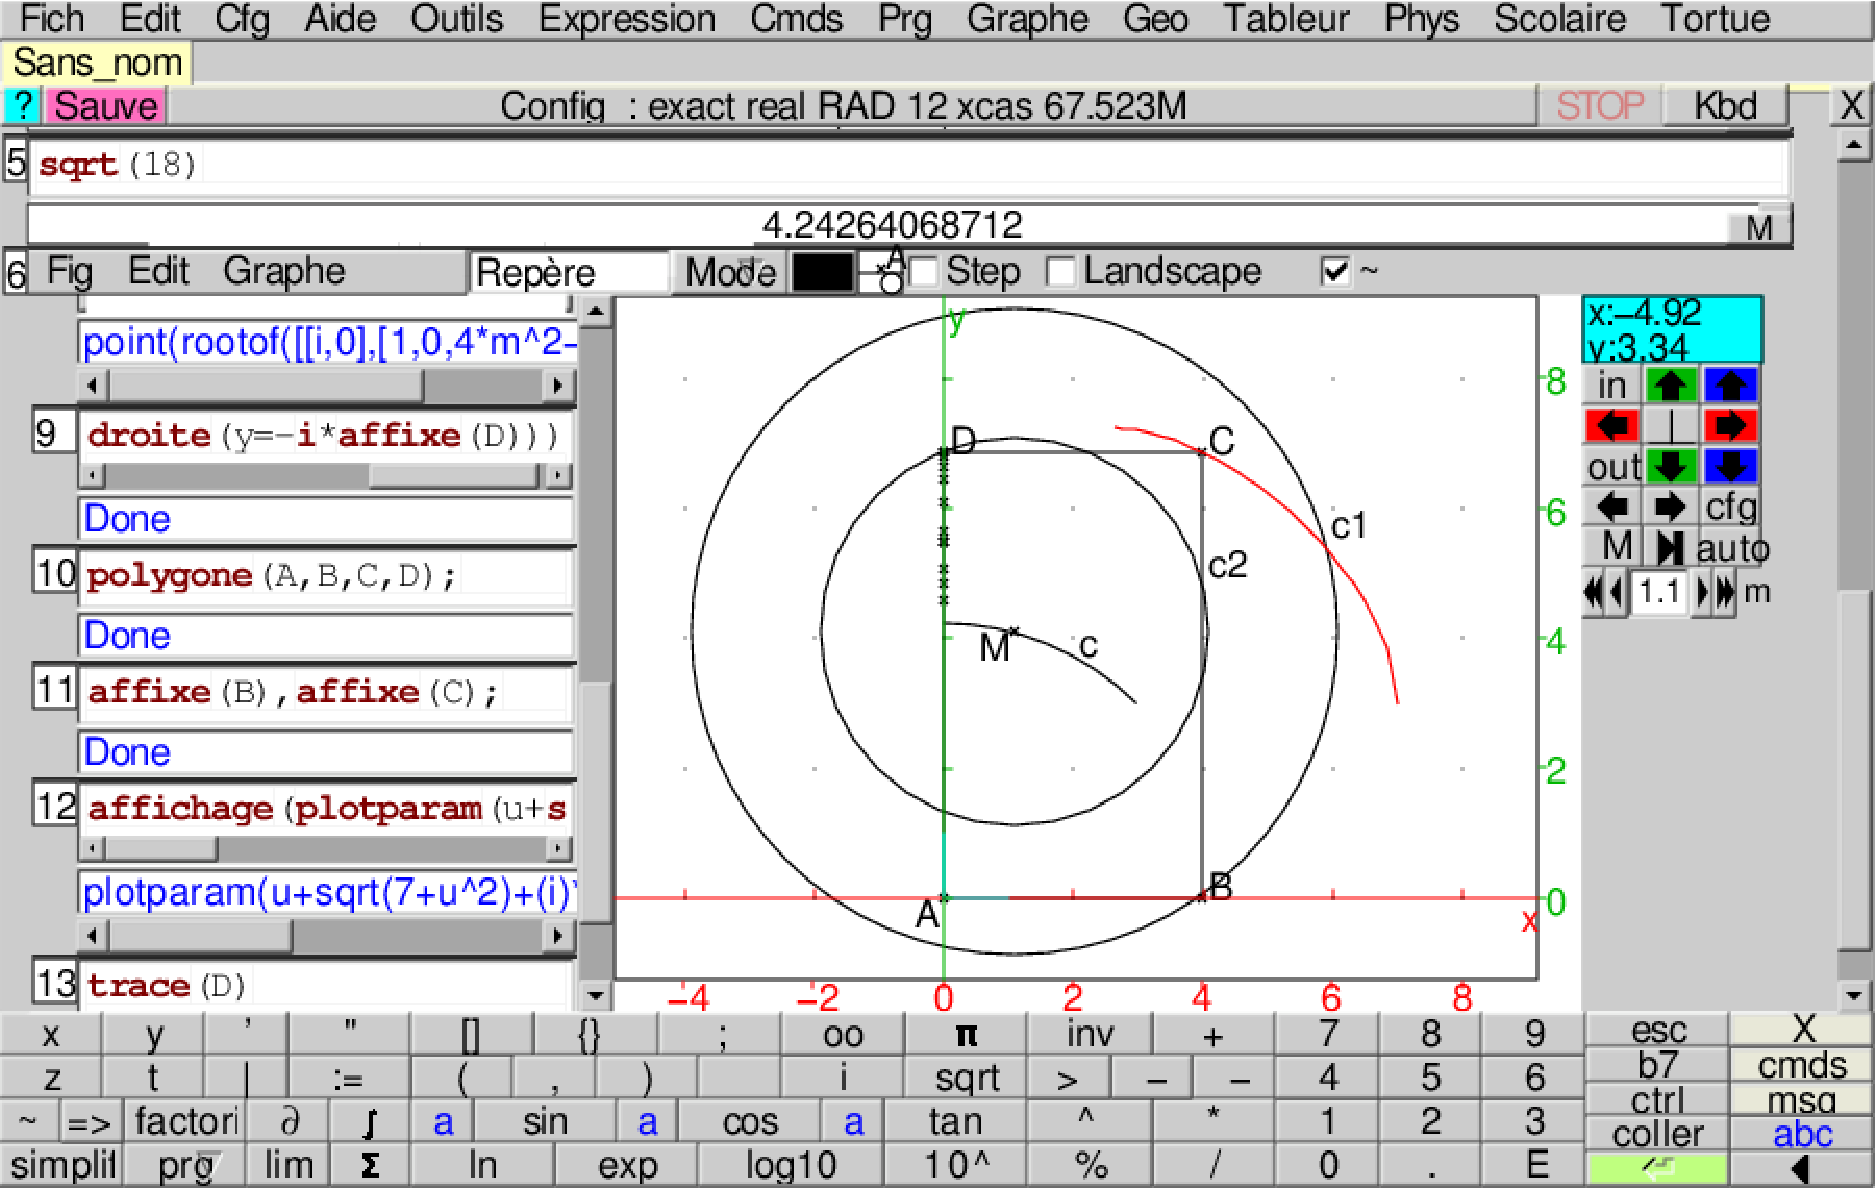
\includegraphics[width=\textwidth]{recta345}
{\bf Remarque}\\
Le probl\`eme est plus facile si on modifie les conditions.\\ 
On cherche les conditions que doivent v\'erifier $x$ et $y$ pour que l'on puisse
construire un point $M$, de coordonn\`ees $(x,y)$, \`a l'int\'erieur du 
rectangle v\'erifiant :\\
$MD=3$, $MC=5$ et $MB=4$.\\ 
On a alors :\\
$x^2+(y-b)^2=9$
$(x-a)^2+(y-b)^2=25$
$(x-a)^2+y^2=16$
Donc :\\
$x^2+(y-b)^2-(x-a)^2-(y-b)^2+(x-a)^2+y^2=x^2+y^2=0$
Donc $x=0$, $y=0$ et $M$ se trouve en $A$.\\
Le rectangle a alors comme dimension $a=4$ et $b=3$. 
\section{Une autre construction avec un triangle \'equilat\'eral}
Soit un triangle \'equilat\'eral $ABC$ tel que $AB=a$.\\
On cherche la valeur de $a$ pour que l'on puisse
construire un point $M$ \`a l'int\'erieur du triangle $ABC$ tel que
$MA=4$, $MB=5$ et $MC=3$.\\ 
Faire la construction de $ABC$ et calculer les aires des 4 triangles :\\
$ABC$, $ABM$, $ACM$, $BCM$.
\begin{center}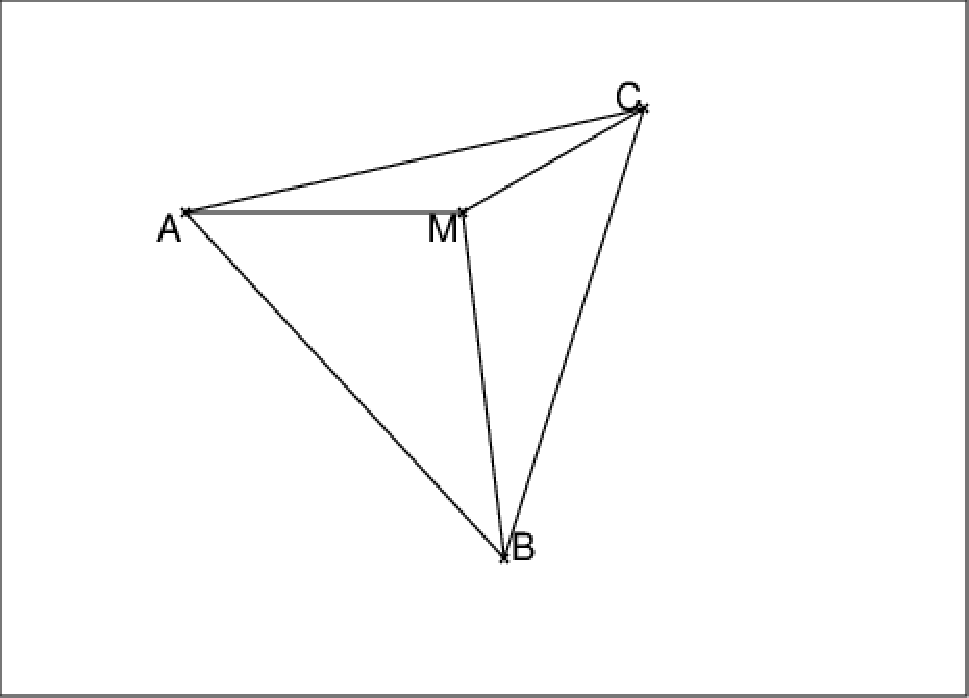
\includegraphics[width=8cm]{equi345}\end{center}
On pourra effectuer la rotation de centre $A$ et d'angle $\pi/3$ qui 
transforme $M$ en $N$.\\

{\bf La solution}\\
Consid\'erons la rotation de centre $A$ et d'angle $\pi/3$ qui transforme $M$ 
en $N$.\\
Le triangle $AMN$ est isoc\`ele de sommet $A$ et on a :\\
$\widehat{MAN}=\widehat{MAC}+\widehat{CAN}=\widehat{MAC}+\widehat{BAM}=\widehat{BAC}=\pi/3$\\
Donc le triangle $AMN$ est \'equilat\'eral et $MN=4$.\\
Le triangle $CNM$ a donc pour c\^ot\'es  : $CM=3$, $MN=4$, $CN=5$.\\
Le triangle $CNM$  est donc rectangle en $M$. et l'angle $\widehat{CMA}=5\pi/6$.\\
On a donc puisque $\cos(5\pi/6)=-\sqrt 3/2$, $MC=3$ et $AM=4$ :\\
$a^2=AC^2=3^2+4^2-2*3*4*(-\sqrt 3/2)=25+12\sqrt 3$.\\
{\bf La construction}\\
On tape :
\begin{verbatim}
C:=point(3);
A:=point(-4*sqrt(3)/2+4*i/2,affichage=quadrant2);
B:=rotation(C,pi/3,A);
triangle(A,B,C);
M:=point(0);
triangle_equilateral(A,M,N,affichage=1);
segment(B,M);
segment(C,M);
\end{verbatim}
On obtient :\\
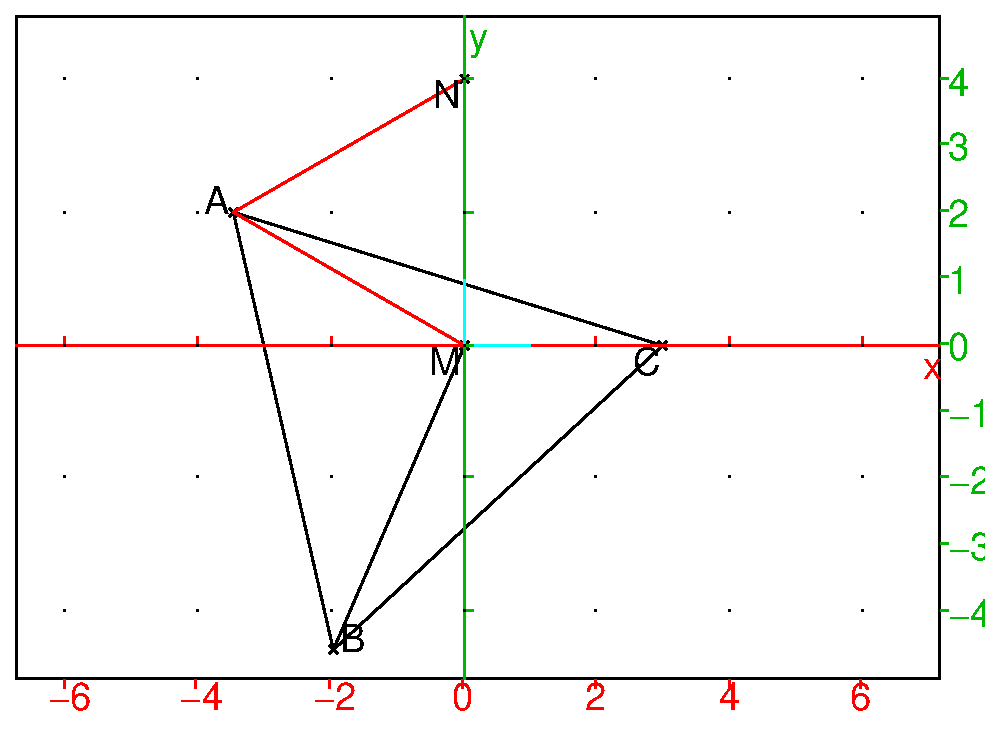
\includegraphics[width=\textwidth]{equi345c}
On v\'erifie, on tape :\\
{\tt normal(longueur(A,M),longueur(B,M))}\\
On obtient :\\
{\tt 4,5}\\
{\bf Calcul des aires \`a l'aide d'un puzzle}\\
On consid\`ere 2 exemplaires du triangle \'equilat\'eral $ABC$ d\'efini 
ci-dessus. On d\'ecoupe un des exemplaires en 3 morceaux qui sont les triangles
$ABM$, $BCM$ et  $AMC$. On obtient donc un puzzle avec les 4 pi\`eces :\\ 
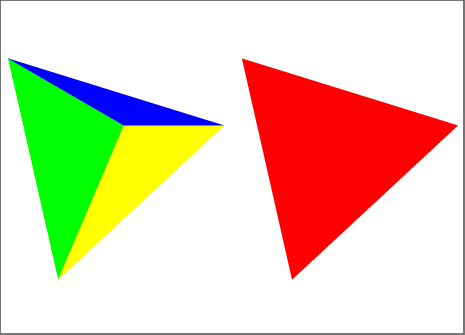
\includegraphics[width=\textwidth]{equi345p}\\
On r\'ealise alors avec ces 4 pi\`eces l'octogone :\\
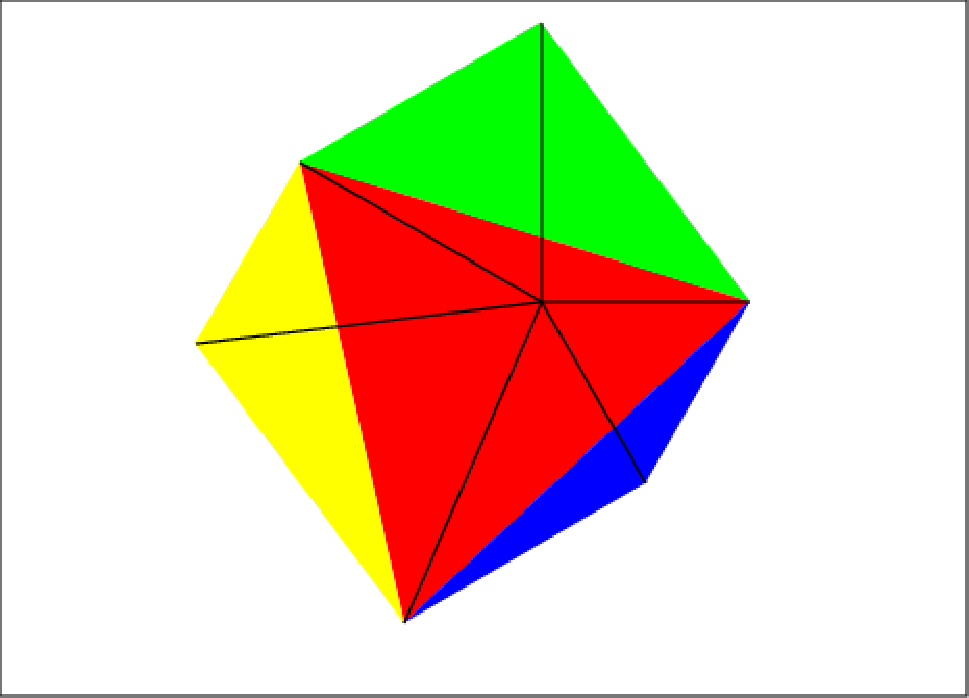
\includegraphics[width=\textwidth]{equi345pp}\\
On a trac\'e les segments joignant $M$ au sommet de l'octogone.\\
Cet octogone est compse de 3 triangles rectangles de c\^ot\'es 3,4,5 et de 
3 triangles \`equilat\'eraux de c\^ot\'es respectifs 3,4 et 5.
On a donc si $S$ est l'aire de $ABC$ :\\
$2S=a^2\sqrt 3/2=3*3*2+(9+16+25)\sqrt 3/4=18+25\sqrt 3/2$\\
Donc $S=9+25\sqrt 3/4$ et on retrouve que $a^2=25+12\sqrt 3$\\
Soient $s_1,s_2,s_3,s_4$ les aires des triangles de couleurs 1 (rouge),2(vert),
3(jaune),4(bleu).\\
On va donc r\'esoudre le syst\`eme lin\'eaire :\\
$[s_1-s_2-s_3-s_4=0,s_2+s_3=6+25\sqrt 3/4,s_2+s_4=9\sqrt 3/4+6,s_3+s_4=4\sqrt 3+6]$\\
On tape :\\
{\tt linsolve([s1-s2-s3-s4=0,s2+s3=6+25*sqrt(3)/4,\\s2+s4=9*sqrt(3)/4+6,s3+s4=4*sqrt(3)+6],[s1,s2,s3,s4])}\\
On obtient :\\
{\tt [(sqrt(3)*25+36)/4,(sqrt(3)*9+12)/4,sqrt(3)*4+3,3]}\\
On a tap\'e pour obtenir l'octogone :
\begin{verbatim}
triangle(A,B,C,affichage=1+rempli);
triangle(A,C,N,affichage=2+rempli);
P:=rotation(C,pi/3,M):;
Q:=rotation(B,pi/3,M):;
triangle(B,C,P,affichage=4+rempli))
triangle(B,A,Q,affichage=3+rempli);
\end{verbatim}
\section{Les transformations}
Les transformations ci-dessous peuvent toujours \^etre consid\'er\'ees, soit 
comme des fonctions (les arguments sont les param\`etres servant \`a d\'efinir 
la transformation), soit comme agissant sur le dernier argument (les arguments 
sont les param\`etres servant \`a d\'efinir 
la transformation et alorsl'objet g\'eom\'etrique \`a 
transformer est mis comme dernier param\`etre).

\subsection{La translation}\index{translation}
\'Etant donn\'e trois points {\tt A, B, C} le point :\\
{\tt translation(C-B,A)} est le transform\'e du point {\tt A} dans la 
translation de vecteur ${\tt \overrightarrow{BC}}$.\\
On a aussi {\tt t:=translation(C-B)} est la translation de vecteur ${\tt \overrightarrow{BC}}$ .\\
On \'ecrira alors {\tt t(A)} pour d\'esigner le transform\'e du point {\tt A} 
dans la translation {\tt t} de vecteur ${\tt \overrightarrow{BC}}$.\\
Par exemple si :\\
{\tt D:=t(A)} ou si\\
{\tt D:=translation(C-B,A)} on a :\\
${\tt \overrightarrow{AD}=\overrightarrow{BC}}$.\\
{\bf Activit\'e}\\
Cr\'eer un polygone quelconque {\tt ABCDE}.\\  
Cr\'eer un point  {\tt F} \`a l'ext\'erieur de ce polygone.\\
Construire le polygone {\tt FGHJK} translat\'e de {\tt ABCDE} dans la translation de vecteur ${\tt \overrightarrow {AF}}$.\\
Faites bouger le point {\tt A} et observer.\\
Faites bouger le point {\tt F} et observer.
\subsection{L'homoth\'etie}\index{homothetie}
\'Etant donn\'e deux points {\tt A, B} et un nombre r\'eel $k$, le point :\\
{\tt homothetie(B,k,A)} est le transform\'e du point {\tt A} dans 
l'homoth\'etie de centre {\tt B} et de rapport $k$.\\
On a aussi {\tt h:=homothetie(B,k)} est l'homoth\'etie de centre {\tt B} et de 
rapport $k$.\\
Par exemple si :\\
{\tt C:=h(A)} ou si\\
{\tt C:=homothetie(B,2,A)}, {\tt C} est tel que 
${\tt \overline{BC}=2*\overline{BA}}$\\
{\bf Activit\'e}\\
Cr\'eer un polygone quelconque {\tt ABCDE}.\\  
Cr\'eer un point  {\tt F} \`a l'ext\'erieur de ce polygone.\\
Construire le polygone {\tt GHJKL} homoth\'etique de {\tt ABCDE} dans 
l'homoth\'etie de vecteur centre {\tt F} et de rapport 2.\\
Faites bouger le point {\tt A} et observer.\\
Faites bouger le point {\tt F} et observer.
\subsection{La sym\'etrie droite et la sym\'etrie point}\index{symetrie}
\'Etant donn\'e trois points {\tt A, B, C} le point :\\
{\tt symetrie(droite(B,C),A)} est le transform\'e du point {\tt A} dans la
sym\'etrie par rapport \`a la droite $BC$,\\
On a aussi {\tt sd:=symetrie(droite(B,C))} est la sym\'etrie par rapport \`a 
la droite $BC$,\\
{\tt symetrie(B,A)} est le transform\'e du point {\tt A} dans la
sym\'etrie de centre {\tt B}.\\
On a aussi {\tt sp:=symetrie(B)} est la sym\'etrie de centre {\tt B}.
On peut aussi comme exercice de programmation d\'efinir les fonctions 
{\tt Symetrie\_point} {\tt Symetrie\_droite} ({\tt symetrie} est la commande de
{\tt Xcas} qui r\'ealise ces 2 fonctions).\\ 
On tape ({\tt A} et {\tt M} sont des points et {\tt d} est une droite) :\\
{\tt Symetrie\_point((A,M)):=A+(A-M)}\\
{\tt Symetrie\_droite(d,M):= \{local N:=inter\_unique(Perpendiculaire(M,d),d);Symetrie\_point(N,M);\}}
\subsection{La rotation}\index{rotation}
\'Etant donn\'e deux points {\tt A, B} et un r\'eel $u$, le point :\\
{\tt rotation(B,u,A)} est le transform\'e du point {\tt A} dans la 
rotation de centre {\tt B} et d'angle de mesure $u$ radians (ou degr\'es selon 
la configuration du {\tt CAS} menu {\tt Cfg->Configuration du CAS}).\\
On a aussi {\tt r:=rotation(B,u)} est la rotation de centre {\tt B} et d'angle 
de mesure $u$ radians (ou degr\'es selon la Configuration du {\tt CAS} menu
{\tt Cfg}).
\subsection{La projection}\index{projection}
\'Etant donn\'e trois points {\tt A, B, C} le point :\\
{\tt projection(droite(B,C),A)} est la projection orthogonale du point {\tt A}
 sur la droite $BC$.\\
On a aussi {\tt p:=projection(droite(B,C))} est la projection orthogonale sur 
la droite $BC$.
\subsection{La similitude}\index{similitude}
\'Etant donn\'e deux points {\tt A, B}, un r\'eel $k$ et un r\'eel $u$, 
le point :\\
{\tt similitude(B,k,u,A)} est le transform\'e du point {\tt A} dans la 
similitude de centre {\tt  B}, de rapport $k$ et d'angle mesure $u$ radians 
(ou degr\'es selon la configuration du {\tt CAS} menu 
{\tt Cfg->Configuration du CAS}).\\
On a aussi {\tt s:=similitude(B,k,u)} est la similitude de centre {\tt B}, de 
rapport $k$ et d'angle mesure $u$ radians (ou degr\'es selon la configuration 
du {\tt CAS} menu {\tt Cfg->Configuration du CAS}).

\subsection{L'inversion}\index{inversion}
\'Etant donn\'e deux points {\tt A, B}, un r\'eel $k$ le point :\\
{\tt inversion(C,k,A)} est le transform\'e du point {\tt A} dans l'inversion
 de centre  {\tt C}, de rapport $k$.\\
 Par exemple si :\\
{\tt A1:=inversion(C,2,A)}, {\tt A1} est tel que
${\tt \overline{CA1}*\overline{CA}=2}$.\\
{\tt inversion(C,k,M)} est donc le point d\'efini par:\\
{\tt point(C+k*conj(inv(M-C)))}\\
On a aussi {\tt inver:=inversion(C,k)} est l'inversion de centre  {\tt C}, 
de rapport $k$.

\section{Les lieux g\'eom\'etriques}\index{lieu}
L'instruction {\tt lieu} permet de tracer le lieu d'un point {\tt M}, lorsque 
ce point {\tt M} est fonction d'un point {\tt P} pouvant se d\'eplacer sur un 
objet g\'eom\'etrique {\tt G} et si on a d\'efini {\tt P} par 
 {\tt P:=element(G)}).\\
 {\bf Remarque} :\\
Il faut que les param\`etres de {\tt lieu} soient des noms de variables.\\
Donc pour obtenir le lieu d'un point {\tt M}, il faut avoir d\'efini 
ce point par une affectation \`a un nom de variable, par exemple 
{\tt M:=...}.\\
On \'ecrit alors :\\
  {\tt lieu(M,P)}
\subsection{Des exemples de lieux}
{\bf Exemple 1} :\\
Lieu du centre de gravit\'e du triangle $ABC$ quand $A$ se d\'eplace
sur une parall\`ele \`a $BC$.\\ 
Ici on cherche le lieu du centre de gravit\'e du triangle $PBC$ lorsque $P$
 se d\'eplace sur la parall\`ele \`a $BC$  passant par $A$.\\
On clique pour obtenir trois points  {\tt A, B, C} et on tape :
\begin{verbatim}
D:=parallele(A,droite(B,C)); 
P:=element(D);
G:=isobarycentre(P,B,C);  
lieu(G,P);
\end{verbatim}
{\tt lieu(G,P)} trace le lieu du point {\tt G} en fonction de {\tt P}.\\
Si l'on veut pouvoir anim\'ee la figure on tape la liste des instructions 
qui se trouve dans le fichier {\tt lieu1}, on clique pour obtenir
 trois points  {\tt A, B, C} puis, on fait 
{\tt Charger session} du 
menu {\tt Fich} de {\tt Xcas} et on selectionne {\tt lieu1} du r\'ep\'ertoire 
{\tt examples/geo} pour ex\'ecuter ce fichier) :\\
Ou on clique pour cr\'eer trois points {\tt A, B, C} et on tape :
\begin{verbatim}
D:=parallele(A,droite(B,C)); 
t:=element(-5..5)
P:=element(D,t);
G:=isobarycentre(P,B,C);  
lieu(G,P);
\end{verbatim}
ainsi lorsqu'on d\'eplace la barre verticale indiquant la valeur de {\tt t},
on voit se d\'eplacer les deux points {\tt P} et {\tt G} simultan\'ement.\\
{\bf Exemples 2 et 3} :\\
Soient deux points  {\tt A} et {\tt  B} et {\tt C1} le cercle 
de diam\`etre {\tt A B}. Soit {\tt O} le centre de ce cercle et {\tt C} un point variable de ce cercle.\\
Soit {\tt N} l'intersection de la tangente en {\tt C}
\`a {\tt C1} avec la parall\`ele \`a {\tt AC} passant par {\tt O}.\\
Trouver le lieu de {\tt N} quand {\tt C} varie.\\

La liste des instructions pour trouver ce lieu se trouve dans le 
fichier {\tt lieu2}, on clique pour obtenir deux points  {\tt A, B} puis, on 
fait {\tt Charger session} du 
menu {\tt Fich} de {\tt Xcas} et on selectionne {\tt lieu2} du r\'ep\'ertoire 
{\tt examples/geo} pour ex\'ecuter ce fichier.\\
Ou on clique pour cr\'eer deux points {\tt A, B} et on tape :
\begin{verbatim}
C1:=cercle(A,B);
O:=milieu(A,B);
C:=element(C1);
T:=tangent(C1,C);
D2:=parallele(O,droite(A,C));
M:=inter(T,D2);
N:=M[0];
lieu(N,C);
\end{verbatim}
{\bf Attention} {\tt M} est une liste ayant un seul \'el\'ement et 
on ne peut pas \'ecrire {\tt lieu(M[0],C)} car {\tt M[0]} n'est pas un nom de 
variable.\\
On peut aussi \'ecrire des instructions  sans utiliser la fonction 
{\tt tangent} et en rajoutant {\tt t:=element(0..2*pi);} (c'est le fichier 
{\tt lieu3}) :\\
On clique pour cr\'eer deux points {\tt A, B}.
\begin{verbatim}
C1:=cercle(A,B);
O:=milieu(A,B);
t:=element(0..2*pi);
C:=element(C1,t);
D1:=perpendiculaire(C,droite(O,C));
D2:=parallele(O,droite(A,C));
M:=inter(D1,D2);
N:=M[0];
lieu(N,C);
\end{verbatim}
Les triangles $NOC$ et $NOB$ sont \'egaux car leurs angles $\widehat{O}$ sont
\'egaux \`a l'angle $\widehat{CAB}$  et \`a l'angle $\widehat{OCA}$. 
Donc $NB$ est perpendiculaire \`a $AB$.\\
La r\'eciproque est \'evidente car si {\tt N} se trouve sur la perpendiculaire
 \`a {\tt AB} en {\tt B}, on m\'ene par {\tt N} l'autre tangente au cercle pour
 d\'efinir le point {\tt C}.\\
 Les triangles rectangles {\tt NOC} et {\tt NOB} sont
 \'egaux et donc {\tt ON} est parall\`ele \`a {\tt AC}.\\ 
{\bf Exemple 4} :\\
Une droite variable {\tt D1} coupe les cot\'es {\tt AB,AC,BC} du triangle 
{\tt ABC} en {\tt D,E,M}.\\
Les cercles circonscrits aux triangles {\tt BDM} et {\tt ECM} se coupent en 
{\tt P} et {\tt M}. Trouver le lieu de {\tt P} quand {\tt D1} varie.\\
On peut faire \'ex\'ecuter le fichier {\tt lieu4} (on clique pour obtenir trois points  {\tt A, B, C} puis on fait {\tt Charger session} du 
menu {\tt Fich} de {\tt Xcas} et on selectionne {\tt lieu4} du r\'ep\'ertoire 
{\tt examples/geo} pour ex\'ecuter ce fichier) ou,\\
on clique pour obtenir trois points  {\tt A, B, C} et on tape :
\begin{verbatim} 
Triangle(A,B,C);
u:=element(-4..4);
M:=element(droite(B,C),u);
D:=element(droite(A,B));
D1:=droite(D,M);
E:=(inter(droite(A,C),D1))[0];
C1:=circonscrit(B,D,M);
C2:=circonscrit(E,C,M);
L:=inter(C1,C2);
if (affixe(L[0])==affixe(M)) {Q:=L[1];} else {Q:=L[0];};
P:=Q;
lieu(P,M);
\end{verbatim}
On remarquera que l'on est oblig\'e d'utiliser un point interm\'ediaire {\tt Q}
pour pouvoir d\'efinir {\tt P} par une affectation.\\
Le lieu de $P$ est le cercle circonscrit au triangle $ABC$ car l'angle
l'angle $\widehat{P}$ du triangle $PBC$ est \'egal \`a l'angle $\widehat{A}$
du triangle $ABC$ en \'ecrivant des \'egalit\'es d'angles inscrits.\\
{\bf Exemple 5} :\\
Lieu de l'orthocentre du triangle $ABC$ quand $A$ se d\'eplace
sur une parall\`ele \`a $BC$.\\ 
Ici on cherche le lieu de l'orthocentre du triangle $MBC$ lorsque $M$
 se d\'eplace sur la parall\`ele \`a $BC$  passant par $A$.\\
On peut faire \'ex\'ecuter le fichier {\tt lieu5} (on clique pour obtenir
 trois points  {\tt A, B, C} puis, on fait {\tt Charger session} du 
menu {\tt Fich} de {\tt Xcas} et on selectionner {\tt lieu5} du r\'ep\'ertoire 
{\tt examples/geo} pour ex\'ecuter ce fichier) ou,\\
on clique pour obtenir trois points  {\tt A,B,C} et on tape :
\begin{verbatim}
D:=parallele(A,droite(B,C));
M:=element(D);
H:=(inter(perpendiculaire(M,droite(C,B)),
          perpendiculaire(C,droite(M,B))))[0] ;
lieu(H,M);
\end{verbatim}
Le lieu est une parabole passant par $B$ et $C$ et de sommet $S$
orthocentre du triangle isoc\`ele $PBC$ ($P$ sur la m\'ediatrice de 
$BC$ et sur la droite $D$). On peut \`a la main avoir assez facilement 
l'\'equation de cette parabole ...mais trouver ce lieu en g\'eom\'etrie pure 
est plus difficle!
\subsection{D'autres exemples de lieux}
{\bf Exemple 1} :\\
Lieu du centre de gravit\'e du triangle $ABC$ quand $A$ se d\'eplace
sur une parall\`ele \`a $BC$.\\ 
Ici on cherche le lieu du centre de gravit\'e du triangle $PBC$ lorsque $P$
 se d\'eplace sur la parall\`ele \`a $BC$  passant par $A$.\\
On clique pour obtenir trois points  {\tt A, B, C} et on tape :
\begin{verbatim}
D:=parallele(A,droite(B,C)); 
P:=element(D);
G:=isobarycentre(P,B,C);  
lieu(G,P);
\end{verbatim}
{\tt lieu(G,P)} trace le lieu du point {\tt G} en fonction de {\tt P}.\\
Si l'on veut pouvoir anim\'ee la figure on tape la liste des instructions 
qui se trouve dans le fichier {\tt lieu1}, on clique pour obtenir
 trois points  {\tt A, B, C} puis, on fait 
{\tt Charger session} du 
menu {\tt Fich} de {\tt Xcas} et on selectionne {\tt lieu1} du r\'ep\'ertoire 
{\tt examples/geo} pour ex\'ecuter ce fichier) :\\
Ou on clique pour cr\'eer trois points {\tt A, B, C} et on tape :
\begin{verbatim}
A:=point([-3,3/2,'affichage'=0]);
B:=point([-1,-3/2,'affichage'=0]);
C:=point([3,9/4,'affichage'=0]);
D:=parallele(A,droite(B,C)); 
P:=element(D);
G:=isobarycentre(P,B,C);  
lieu(G,P);
\end{verbatim}
ainsi lorsqu'on d\'eplace la barre verticale indiquant la valeur de {\tt t},
on voit se d\'eplacer les deux points {\tt P} et {\tt G} simultan\'ement.\\
{\tt lieu(G,P);} renvoie droite(y=((15*x)/16+17/16))
{\bf Exemples 2 et 3} :\\
Soient deux points  {\tt A} et {\tt  B} et {\tt C1} le cercle 
de diam\`etre {\tt A B}. Soit {\tt O} le centre de ce cercle et {\tt C} un point variable de ce cercle.\\
Soit {\tt N} l'intersection de la tangente en {\tt C}
\`a {\tt C1} avec la parall\`ele \`a {\tt AC} passant par {\tt O}.\\
Trouver le lieu de {\tt N} quand {\tt C} varie.\\

La liste des instructions pour trouver ce lieu se trouve dans le 
fichier {\tt lieu2}, on clique pour obtenir deux points  {\tt A, B} puis, on 
fait {\tt Charger session} du 
menu {\tt Fich} de {\tt Xcas} et on selectionne {\tt lieu2} du r\'ep\'ertoire 
{\tt examples/geo} pour ex\'ecuter ce fichier.\\
Ou on clique pour cr\'eer deux points {\tt A, B} et on tape :
\begin{verbatim}
C1:=cercle(A,B);
O:=milieu(A,B);
C:=element(C1);
T:=tangent(C1,C);
D2:=parallele(O,droite(A,C));
M:=inter(T,D2);
N:=M[0];
lieu(N,C);
\end{verbatim}
{\bf Attention} {\tt M} est une liste ayant un seul \'el\'ement et 
on ne peut pas \'ecrire {\tt lieu(M[0],C)} car {\tt M[0]} n'est pas un nom de 
variable.\\
On peut aussi \'ecrire des instructions  sans utiliser la fonction 
{\tt tangent} et en rajoutant {\tt t:=element(0..2*pi);} (c'est le fichier 
{\tt lieu3}) :\\
On clique pour cr\'eer deux points {\tt A, B}.
\begin{verbatim}
C1:=cercle(A,B);
O:=milieu(A,B);
C:=element(C1);
D1:=perpendiculaire(C,droite(O,C));
D2:=parallele(O,droite(A,C));
M:=inter(D1,D2);
N:=M[0];
lieu(N,C);
\end{verbatim}
{\tt lieu(N,C)} renvoie {\tt droite(y=((2*x)/3-5/6))}\\
Les triangles $NOC$ et $NOB$ sont \'egaux car leurs angles $\widehat{O}$ sont
\'egaux \`a l'angle $\widehat{CAB}$  et \`a l'angle $\widehat{OCA}$. 
Donc $NB$ est perpendiculaire \`a $AB$.\\
La r\'eciproque est \'evidente car si {\tt N} se trouve sur la perpendiculaire
 \`a {\tt AB} en {\tt B}, on m\'ene par {\tt N} l'autre tangente au cercle pour
 d\'efinir le point {\tt C}.\\
 Les triangles rectangles {\tt NOC} et {\tt NOB} sont
 \'egaux et donc {\tt ON} est parall\`ele \`a {\tt AC}.\\ 
{\bf Exemple 4} :\\
Une droite variable {\tt D1} coupe les cot\'es {\tt AB,AC,BC} du triangle 
{\tt ABC} en {\tt D,E,M}.\\
Les cercles circonscrits aux triangles {\tt BDM} et {\tt ECM} se coupent en 
{\tt P} et {\tt M}. Trouver le lieu de {\tt P} quand {\tt D1} varie.\\
On peut faire \'ex\'ecuter le fichier {\tt lieu4} (on clique pour obtenir trois points  {\tt A, B, C} puis on fait {\tt Charger session} du 
menu {\tt Fich} de {\tt Xcas} et on selectionne {\tt lieu4} du r\'ep\'ertoire 
{\tt examples/geo} pour ex\'ecuter ce fichier) ou,\\
on clique pour obtenir trois points  {\tt A, B, C} et on tape :
\begin{verbatim} 
triangle(A,B,C);
u:=element(-4..4);
M:=element(droite(B,C),u);
D:=element(droite(A,B));
D1:=droite(D,M);
E:=(inter(droite(A,C),D1))[0];
C1:=circonscrit(B,D,M);
C2:=circonscrit(E,C,M);
L:=inter(C1,C2);
if (affixe(L[0])==affixe(M)) {Q:=L[1];} else {Q:=L[0];};
P:=Q;
lieu(P,M);
\end{verbatim}
On remarquera que l'on est oblig\'e d'utiliser un point interm\'ediaire {\tt Q}
pour pouvoir d\'efinir {\tt P} par une affectation.\\
Le lieu de $P$ est le cercle circonscrit au triangle $ABC$ car l'angle
l'angle $\widehat{P}$ du triangle $PBC$ est \'egal \`a l'angle $\widehat{A}$
du triangle $ABC$ en \'ecrivant des \'egalit\'es d'angles inscrits.\\
{\bf Exemple 5} :\\
Lieu de l'orthocentre du triangle $ABC$ quand $A$ se d\'eplace
sur une parall\`ele \`a $BC$.\\ 
Ici on cherche le lieu de l'orthocentre du triangle $MBC$ lorsque $M$
 se d\'eplace sur la parall\`ele \`a $BC$  passant par $A$.\\
On peut faire \'ex\'ecuter le fichier {\tt lieu5} (on clique pour obtenir
 trois points  {\tt A, B, C} puis, on fait {\tt Charger session} du 
menu {\tt Fich} de {\tt Xcas} et on selectionner {\tt lieu5} du r\'ep\'ertoire 
{\tt examples/geo} pour ex\'ecuter ce fichier) ou,\\
on clique pour obtenir trois points  {\tt A,B,C} et on tape :
\begin{verbatim}
D:=parallele(A,droite(B,C));
M:=element(D);
H:=(inter(perpendiculaire(M,droite(C,B)),
          perpendiculaire(C,droite(M,B))))[0] ;
lieu(H,M);
\end{verbatim}
Le lieu est une parabole passant par $B$ et $C$ et de sommet $S$
orthocentre du triangle isoc\`ele $PBC$ ($P$ sur la m\'ediatrice de 
$BC$ et sur la droite $D$). On peut \`a la main avoir assez facilement 
l'\'equation de cette parabole ...mais trouver ce lieu en g\'eom\'etrie pure 
est plus difficle!
\subsection{Des exercices de lieux}
{\bf Exercice1}\\
Soient 2 points fixes $A$ et $B$.\\
On consid\`ere l'ensemble $\Gamma$ des cercles $c$ passant par $A$ et $B$.\\
Pour $c \in \Gamma$, lieu des points $M$ de $c$ qui ont une tangente en $M$
perpendiculaire \`a $AB$.\\
On tape dans un niveau de g\'eom\'etrie 2d (version 1) :
\begin{verbatim}
A:=point(-1);
B:=point(1);
P:=element(droite(x=0));
c:=cercle(P,A-P);
M:=translation(longueur(A,P),P);
N:=translation(-longueur(A,P),P);
lieu(M,P);
lieu(N,P);
\end{verbatim}
ou on tape  dans un niveau de g\'eom\'etrie 2d (version 2) :
\begin{verbatim}
A:=point(-1);
B:=point(1);
assume(u=[0,-5,5,0.1]));
P:=element(droite(x=0),u);
c:=cercle(P,sqrt(u^2+1));
L:=inter(droite(y=u),c);
M:=L[0];
N:=L[1];
lieu(M,u);
lieu(N,u); 
\end{verbatim}
Pour la version 1 (resp pour la version 2) {\tt lieu(M,P);} (resp 
{\tt lieu(M,u);}) renvoie :\\
{\tt plotparam((i)*` t`+sqrt(1+(-` t`)\verb|^|2),` t`=-10.0..10.0)}\\
et pour la version 1 (resp pour la version 2) {\tt lieu(N,P);} (resp 
{\tt lieu(N,u);}) renvoie :\\
{\tt plotparam((i)*` t`-sqrt(1+(-` t`)\verb|^|2),` t`=-10.0..10.0)}\\
et le dessin correspondant :\\
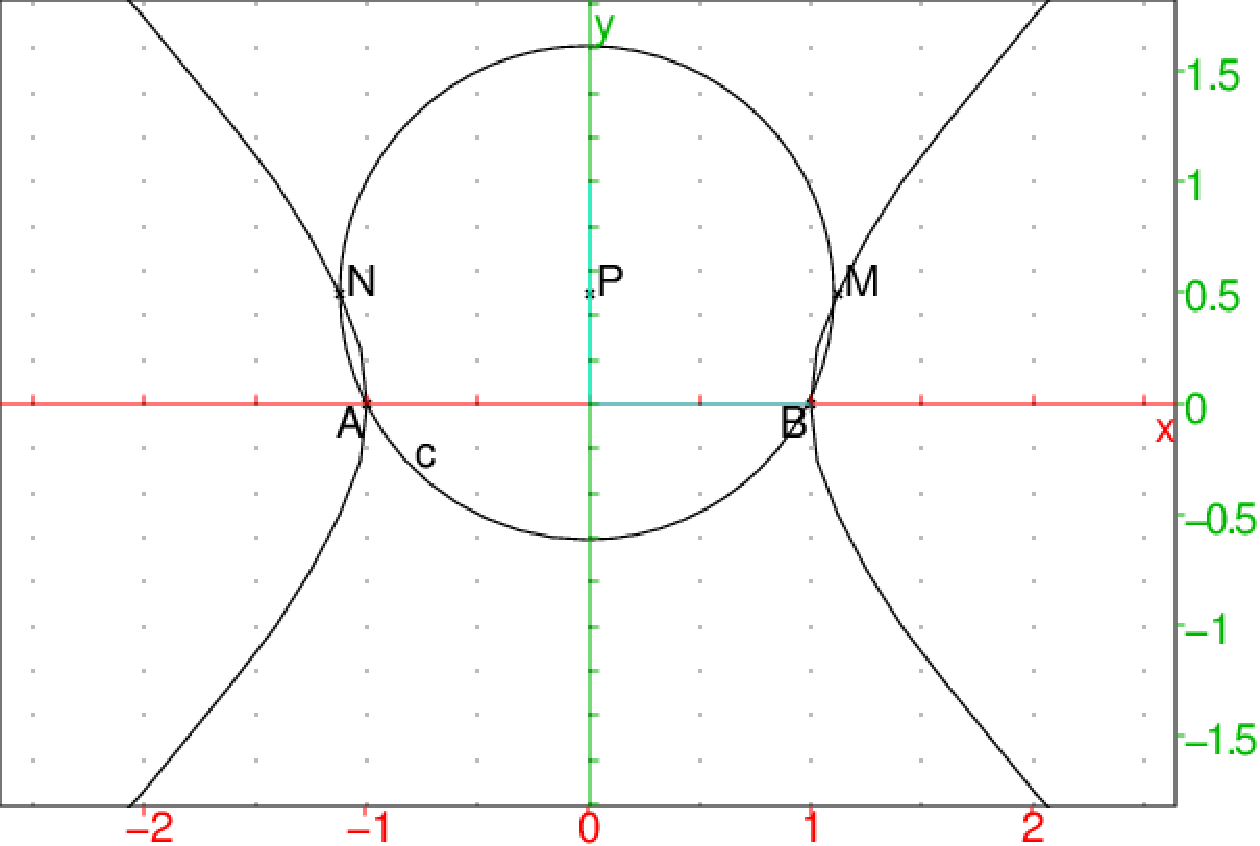
\includegraphics[width=\textwidth]{lieu0}\\

On peut aussi taper en utilisant directement {\tt plotparam} :
\begin{verbatim}
supposons(u=[0,-5,5,0.1])
P:=point(i*u)
c:=cercle(P,sqrt(u^2+1));
L:=inter(droite(y=u),c):;
M:=L[0];N:=L[1];
plotparam(affixe(M),u);
plotparam(affixe(N),u);
\end{verbatim}
On obtient le dessin ci-dessus.\\
%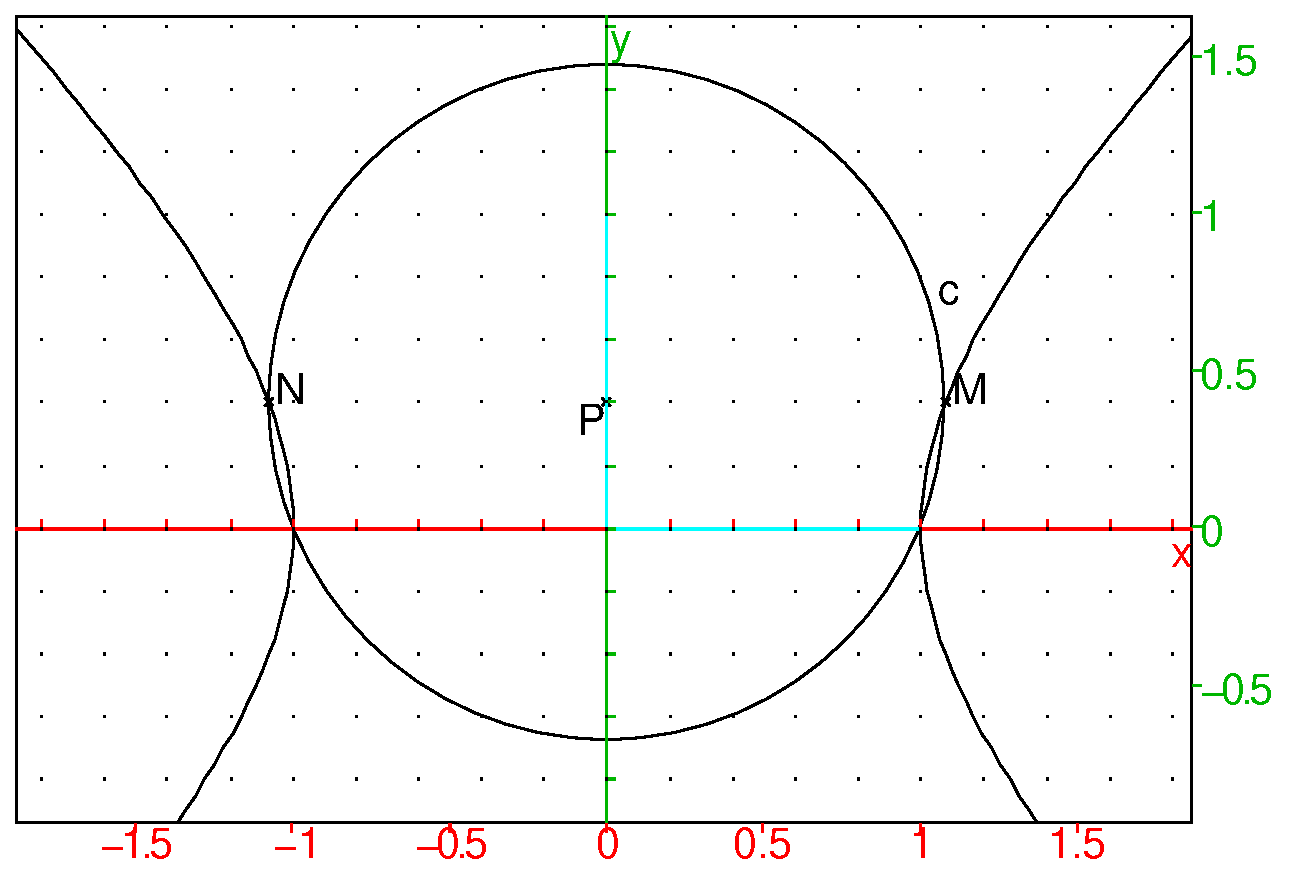
\includegraphics[width=\textwidth]{lieu2}\\
On tape :\\
{\tt affixe(M)}\\
On obtient :\\
{\tt (i)*u+sqrt(u\verb|^|2+1)}\\
On tape :\\
{\tt affixe(N)}\\
On obtient :\\
{\tt (i)*u-sqrt(u\verb|^|2+1)}\\
{\bf Exercice2}\\
Soient un cercle $c$ de centre $O$ et 2 points fixes $A$ et $B$ situ\'es sur un 
diam\`etre de $c$.\\
Soit un diam\`etre variable $PQ$ de $c$.\\
Lieu de $M$ intersection de $AP$ et $BQ$.\\
On tape :
\begin{verbatim}
c:=cercle(0,1)
A:=point(-4);
B:=point(-2);
u:=element(-pi..pi);
P:=element(c,u);
Q:=-P;
M:=inter_unique(droite(A,P),droite(B,Q));
lieu(M,P)
\end{verbatim}
On obtient :\\
{\tt cercle(point(-8/3,0),1/3)}\\
On tape :\\
{\tt droite(A,0);segment(P,A);segment(M,Q)}\\
{\tt segment(0,P);segment(M,point(-8/3))}\\
On obtient le cercle homoth\'etique de $c$ dans l'homoth\'etie de centre $A$ et 
de rapport ici 1/3.\\
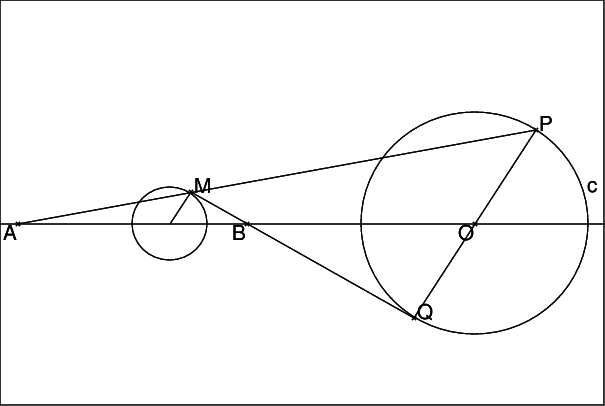
\includegraphics[width=\textwidth]{lieu1}\\
On a en effet en appliquant le th\'eor\'eme de M\'en\'ela\"us au triangle $OAP$ on a :\\
$M,B,Q$ align\'es est \'equivalent \`a :
$\displaystyle \frac{\overline{MA}}{\overline{MP}}\cdot \frac{\overline{QP}}{\overline{QO}}\cdot \frac{\overline{BO}}{\overline{BA}}=1$\\
On a $\displaystyle \frac{\overline{QP}}{\overline{QO}}=2$.
Si $\displaystyle \frac{\overline{BA}}{\overline{BO}}=k$ alors 
$\displaystyle \frac{\overline{MA}}{\overline{MP}}=\frac{k}{2}$ donc \\
$\displaystyle \frac{\overline{AP}}{\overline{AM}}=1+\frac{\overline{MP}}{\overline{AM}}=1-\frac{2}{k}=\frac{k-2}{k}$\\
Ce qui prouve que $M$ se d\'eduit de $P$ dans l'homoth\'etie de centre $A$ et de rapport : $\displaystyle \frac{k}{k-2}$\\
Dans l'exemple on a $k=-1$ donc le rapport de l'homoth\'etie est bien : $\displaystyle \frac{1}{3}$
\section{Figures polygonales}
\subsection{Le triangle}\index{triangle}\index{triangle\_isocele}\index{triangle\_equilateral}\index{triangle\_rectangle}
\'Etant donn\'e trois points {\tt A}, {\tt B} et {\tt C} les commandes 
suivantes permettent de tracer des triangles :
\begin{itemize}
\item Le triangle quelconque\\
{\tt triangle(A,B,C)} trace le triangle $ABC$.
\item Le triangle \'equilat\'eral\\
{\tt triangle\_equilateral(A,B)} trace le triangle \'equilat\'eral direct $ABC$
mais sans d\'efinir le point $C$. Pour d\'efinir $C$, il faut donner un nom 
au triangle (par exemple $T$) et utiliser la commande {\tt sommets(T)} qui 
renvoie la liste des sommets de $T$.\\
 On \'ecrira alors :\\
{\tt T:=triangle\_equilateral(A,B);C:= sommets(T)[2]}.\\
Mais, pour d\'efinir $C$, il est plus facile d'utiliser :\\
{\tt triangle\_equilateral(A,B,C)} qui trace le triangle \'equilat\'eral direct 
$ABC$ en mettant dans la variable {\tt C} le point $C$.
\item Le triangle isoc\`ele\\
On suppose que $c$ d\'esigne la mesure en radians (ou en degr\'es) de l'angle  
$(\overrightarrow {AB},\overrightarrow {AC})$.\\
{\tt triangle\_isocele(A,B,c)} trace (sans d\'efinir le point C) le triangle 
isoc\`ele $ABC$ de sommet $A$, tel que l'angle 
$(\overrightarrow {AB},\overrightarrow {AC})=c$ radians (ou degr\'es).\\ 
{\tt triangle\_isocele(A,B,c,C)} trace le triangle isoc\`ele $ABC$ de sommet 
$A$, tel que l'angle $(\overrightarrow {AB},\overrightarrow {AC})=c$ radians
 (ou degr\'es), en mettant dans la variable {\tt C} le point $C$.\\
On d\'efinit deux points $A$ et $B$ et on tape, par exemple, pour avoir un 
triangle rectangle isoc\'ele $ABC$ :\\
{\tt triangle\_isocele(A,B,pi/2,C)}\\
{\bf Activit\'e}\\
Cr\'eer un segment {\tt AB}.\\
Construire  un triangle isoc\`ele {\tt ABC} de sommet {\tt A} ($AB=AC$) tel 
que l'angle $A$ mesure $30^\circ$=$\frac{\pi}{6}$ radians.\\
Construire  un triangle isoc\`ele {\tt ABD} de sommet {\tt A} ($AB=AD$) tel 
que l'angle $B$ mesure $30^\circ$=$\frac{\pi}{6}$ radians.\\
{\bf R\'eponse}\\
Supposons que l'on a choisi {\tt radian} dans la fen\^etre de configuration du {\tt CAS}.\\
On clique avec la souris pour avoir le segment {\tt AB} puis,
 on ex\'ecute la liste des instructions :\\
%qui se trouve dans {\tt geo9} (faire {\tt Charger session} du 
%menu {\tt Fich} de {\tt Xcas} et selectionner {\tt geo9} du r\'ep\'ertoire 
%{\tt examples/geo} pour ex\'ecuter ce fichier).\\
%Voici le d\'etail de {\tt geo9} :\\
{\tt C:=rotation(A,pi/6,B)} $C$ est le transform\'e de $B$ dans la rotation de
 centre A et d'angle $\frac{\pi}{6}$ radians,\\
{\tt D:=rotation(A,2*pi/3,B)} $D$ est le transform\'e de $B$ dans la rotation de centre A et d'angle $\frac{2*\pi}{3}$ radians (car $\pi-2*\pi/6=2*\pi/3$).
\item Le triangle rectangle\\
{\tt triangle\_rectangle(A,B,k)} trace (sans d\'efinir le point C) le triangle 
$ABC$ rectangle en $A$ tel que  $longueur(A,C)=|k|*longueur(A,B)$ : ce triangle est direct si $k>0$ et indirect sinon.\\
{\tt triangle\_rectangle(A,B,k,C)} trace le triangle $ABC$ rectangle en $A$
tel que  $longueur(A,C)=|k|*longueur(A,B)$, ce triangle est direct si $k>0$ et indirect sinon et met dans la variable {\tt C} le point $C$.\\
Si on suppose que $c$ contient la mesure en radians (ou en degr\'es) de l'angle
 $(\overrightarrow {BA},\overrightarrow {BC})$, on a :\\
{\tt triangle\_rectangle(A,B,tan(c))} ou \\
{\tt triangle\_rectangle(A,B,tan(c),C)} trace le triangle $ABC$ rectangle en $A$
tel que l'angle  $(\overrightarrow {BC},\overrightarrow {BA})=c$ radians (ou 
degr\'es).\\
On remarquera que le troisi\`eme param\`etre a pour valeur absolue $\frac{AC}{AB}$  et que le triangle est direct si il est positif et indirect si il est 
n\'egatif.\\ 
{\bf Activit\'e}\\
Cr\'eer un segment {\tt AB} et un segment {\tt CD}  tels que les 
deux points  {\tt A} et {\tt B} soient en dehors de la
droite $CD$.\\
 Construire  un point {\tt E} sur la droite $CD$ pour que le triangle 
{\tt ABE} soit rectangle en {\tt E} (\^E=$90^\circ$=$\frac{\pi}{2}$ radians).\\
{\bf R\'eponse}\\
$E$ se trouve sur le cercle de diam\`etre $AB$ et sur la droite $CD$.\\
On clique avec la souris pour avoir les segments  {\tt AB} et {\tt CD} puis,
 on ex\'ecute la liste des instructions qui se trouve dans {\tt geo10} (faire 
{\tt Charger session} du 
menu {\tt Fich} de {\tt Xcas} et selectionner {\tt geo10} du r\'ep\'ertoire 
{\tt examples/geo} pour ex\'ecuter ce fichier).\\
Voici le d\'etail de {\tt geo10} :\\
{\tt E:=inter(droite(C,D),cercle(A,B))} est l'intersection de la droite $CD$ 
avec le cercle de diam\`etre $AB$,\\
{\tt E1:=E[0]} est le premier point de cette intersection,\\
{\tt E2:=E[1]} est le deuxi\`eme point de cette intersection,\\
{\tt triangle(E1,A,B)} trace le triangle $ABE1$\\
{\tt triangle(E2,A,B)} trace le triangle $ABE2$\\
Ces deux triangles r\'epondent \`a la question.
\end{itemize}

\subsection{Les quadrilat\`eres}\index{carre}\index{losange}\index{quadrilatere}\index{rectangle}
Les commandes suivantes permettent de tracer des quadrilat\`eres :
\begin{itemize}
\item Le quadrilat\`ere quelconque :\\
On donne 4 points $A,B,C,D$ et on construit le quadrilat\`ere  $ABCD$.\\
On a :\\
{\tt quadrilatere(A,B,C,D)} trace le quadrilat\`ere $ABCD$.

\item Le carr\'e :\\
On donne 2 points $A,B$ et on construit le carr\`e $ABCD$ de sens direct.
On a :\\
{\tt carr\'e(A,B)} trace le carr\`e $ABCD$ de sens direct, mais sans d\'efinir
 les points C et D.\\
{\tt carr\'e(A,B,C,D)} trace le carr\`e $ABCD$ de sens direct, et met dans 
{\tt C} et {\tt D} les points C et D.

\item Le losange :\\
On donne 2 points $A,B$ et une mesure d'angle $t$ et on construit le losange 
$ABCD$ tel que $(\overrightarrow{AB}$,$\overrightarrow{AD})=t$.
On a :\\
{\tt losange(A,B,t)} trace le losange $ABCD$ tel que :\\
($\overrightarrow{AB}$,$\overrightarrow{AD}$)=t, mais sans d\'efinir 
les points $C$ et $D$.\\
{\tt losange(A,B,t,C,D)} trace le losange $ABCD$ tel que :\\
$(\overrightarrow{AB}$,$\overrightarrow{AD})=t$, et met dans 
{\tt C} et {\tt D} les points $C$ et $D$.

\item Le rectangle :\\
On donne  2 points $A,B$ et un r\'eel $k$ et on construit le rectangle $ABCD$ 
(direct si $k>0$ et indirect sinon) tel que  $AD=|k|*AB$.\\
On a :\\
{\tt rectangle(A,B,k)} trace (sans d\'efinir les points  $C$ et $D$) le 
rectangle $ABCD$ tel que $AD=|k|*AB$. 
Ce rectangle est direct si $k>0$ et indirect sinon.\\
{\tt rectangle(A,B,k,C,D)} trace le rectangle $ABCD$ tel que :\\
$AD=|k|*AB$, et met dans {\tt C} et {\tt D} les points $C$ et $D$.
Ce rectangle est direct si $k>0$ et indirect sinon.

\item Le parall\'elogramme :\\
On donne 3 points $A,B,C$ et on construit le e parall\'elogramme $ABCD$ c'est 
\`a dire le point $D$ tel que $\overrightarrow {AD}=\overrightarrow {BC}$.\\
On a :\\
{\tt parallelogramme(A,B,C)} trace le parall\'elogramme $ABCD$.\\
{\tt parallelogramme(A,B,C,D)} trace le parall\'elogramme $ABCD$ et met dans 
{\tt D} le point $D$.

\end{itemize}
\subsection{Les polygones}\index{polygone}
Soient $n$ points (ou $n$ nombres complexes repr\'esentant l'affixe de ces points).\\
{\tt polygone} avec comme argument la liste ou la s\'equence de ces $n$ points.\\ 
{\tt polygone} renvoie et trace le polygone ayant pour sommets ces $n$ points.\\
{\tt polygone(0,1,1+i,i)} trace le carr\'e de sommets 0,1,1+i,i.\\
{\tt polygone(makelist(x->exp(i*pi*x/3),0,5,1))} trace l'hexagone de centre 0 et de sommets 1,$e^{\frac{i*pi}{3}}$...$e^{\frac{5*i*pi}{3}}$
\subsection{Les sommets d'un polygone}\index{sommets}
Les commandes pr\'ec\'edentes peuvent tracer des triangles ou des 
quadrilat\`eres sans avoir tous les sommets, mais on peut avoir besoin des 
sommets de ces triangles ou de ces quadrilat\`eres.\\
Si {\tt T} est un triangle (ou un polygone) {\tt sommets(T)} renvoie la 
liste circulaire des sommets de {\tt T}, ainsi  {\tt sommets(T)[0]} et 
{\tt sommets(T)[3]}
d\'esigne le premier sommet de {\tt T} (attention aux indices!!!).\\
Exemple :\\
On clique pour avoir deux points {\tt A} et {\tt B}.\\
On tape :\\
{\tt T:=triangle\_equilateral(A,B)}\\
{\tt C:=sommets(T)[2]}\\
Ainsi le triangle $ABC$ est \'equilat\'eral.\\
On tape :\\
{\tt Q:=carre(A,B)}\\
{\tt E:=sommets(T)[2]}\\
{\tt F:=sommets(T)[3]}\\
Ainsi, $ABEF$ est un carr\'e.
\subsection{Activit\'es : constructions de quadrilat\`eres}
\begin{itemize}
\item Le parall\'elogramme\\
{\bf Activit\'e}\\
Cr\'eer trois points {\tt A, B, C}.\\
Construire le quatri\`eme sommet  {\tt D} du parall\'elogramme  {\tt ABCD} :
on d\'ecrira trois m\'ethodes de construction du point {\tt D}.\\
 {\bf R\'eponse}\\
1/ $D$ est tel que $\overrightarrow {AD}=\overrightarrow {BC}$.\\
On tape :\\
{\tt D:=A+C-B} (ou encore {\tt D:=translation(C-B,A)}) \\
2/ $AC$ et $BD$ ont m\^eme milieu.\\
On tape :\\
{\tt M:=milieu(A,C)}\\
{\tt D:=symetrie(M,B)}\\
3/ $AD$ est parall\'ele \`a $BC$ et $AB$ est parall\'ele \`a $DC$.\\
On tape :\\
{\tt D1:=parallele(A,droite(B,C))}\\
{\tt D2:=parallele(C,droite(B,A))}\\
{\tt D:=inter(D1,D2)[0]}\\
On peut ensuite v\'erifier avec la commande {\tt parallelogramme}.

\item Le carr\'e\\
{\bf Activit\'e}\\
Cr\'eer un segment {\tt AB}.\\
Construire  un carr\'e de c\^ot\'e {\tt AB} : on d\'ecrira deux m\'ethodes 
de construction du carr\'e et une m\'ethode qui utilise les nombres complexes 
et un petit programme.\\
{\bf R\'eponse}\\
1/ On obtient $C$ et $D$ par rotation.\\
On tape :\\
${\tt C:=rotation(B,-\pi/2,A)}$\\
${\tt D:=rotation(A,\pi/2,B)}$\\
(ou encore {\tt C:=B-i*(A-B)} {\tt D:=A+i*(B-A)})\\
Puis on trace le carr\'e :\\
{\tt segment(A,B);segment(B,C);segment(C,D);segment(D,A);}\\
2/ On obtient $C$ par rotation et $D$ par sym\'etrie .\\
On tape :\\
${\tt C:=rotation(B,-\pi/2,A)}$\\
{\tt M:=milieu(A,C)}\\
{\tt D:=symetrie(M,B)}\\
Puis on trace le carr\'e :\\
{\tt segment(A,B);segment(B,C);segment(C,D);segment(D,A);}\\
3/ On utilise les nombres complexes et on \'ecrit le programme :
\begin{verbatim}
carred(A,B):={
local C,D;
C:=B+i*(B-A);
D:=A+i*(B-A);
return ([segment(A,B),segment(B,C),
         segment(C,D),segment(D,A)]);
};
\end{verbatim}
{\bf Attention}\\
 Lorsque il y a des commandes graphiques interm\'ediaires, elles sont trac\'ees
dans l'\'ecran {\tt DispG}, mais seule la valeur de la fonction (ce qui suit 
{\tt return}) est trac\'ee.
\end{itemize}
On peut ensuite v\'erifier avec la commande {\tt carre}.
\subsection{Un exercice sur la droite des milieux}
\subsubsection{L'exercice}
Soit un quadrilat\`ere quelconque $ABCD$ et $M,N, P, Q$ les milieux respectifs 
de $AB, BC, CD, DA$.
\begin{itemize}
\item Quelle est la nature du quadrilat\`ere $MNPQ$ ?
\item Trouver une condition n\'ecessaire et suffisante pour que le 
quadrilat\`ere $MNPQ$ soit un losange.
\item Trouver une condition n\'ecessaire et suffisante pour que le 
quadrilat\`ere $MNPQ$ soit un rectangle.
\item Trouver une condition n\'ecessaire et suffisante pour que le 
quadrilat\`ere $MNPQ$ soit un carr\'e.
\end{itemize}
\subsubsection{La solution}
Il est conseill\'e de faire une figure avec {\tt Xcas} : on ouvre l'\'ecran de 
g\'eom\'etrie et on clique sur 4 points {\tt A, B, C, E} on modifie la ligne
{\tt E:=...} en {\tt D:=...} puis on tape :
\begin{verbatim}
M:=milieu(A,B);
N:=milieu(C,B);
P:=milieu(C,D);
Q:=milieu(A,D);
quadrilatere(A,B,C,D,couleur=rouge);
segment(A,C,couleur=vert);
segment(B,D,couleur=vert);
quadrilatere(M,N,P,Q);
\end{verbatim}
Puis on se met en mode {\tt Pointer} et on d\'eplace le point {\tt D} avec la 
souris et on observe......\\
Cette session se trouve parmi les exemples sous le nom {\tt milieu.xws}.

La d\'emonstration :
\begin{itemize}
\item $MN$ joint les milieux des c\^ot\'es $AB$ et $BC$ du triangle $ABC$
donc $MN$ est parall\`ele \`a $AC$ et $MN=AC/2$,\\
de m\^eme $PQ$ joint les milieux des c\^ot\'es $AD$ et $DC$ du triangle $ADC$
donc $PQ$ est parall\`ele \`a $AC$ et $PQ=AC/2$.
Le quadrilat\`ere $MNPQ$ est donc un prall\'elogramme puisque ses c\^ot\'es
$MN$ et $PQ$ sont \'egaux et parall\`eles. \\
{\bf Remarque}\\
On a aussi :\\
$MQ$ joint les milieux des c\^ot\'es $AB$ et $AD$ du triangle $DAB$
donc $MQ$ est parall\`ele \`a $BD$ et $MQ=BD/2$ et\\
$NP$ joint les milieux des c\^ot\'es $AB$ et $AD$ du triangle $DCB$
donc $NP$ est parall\`ele \`a $BD$ et $NP=BD/2$.

\item Une condition n\'ecessaire et suffisante pour que le 
prall\'elogramme $MNPQ$ soit un losange est que $MN=NP$.
D'apr\'es la remarque pr\'ec\'edente l'\'egalit\'e $MN=NP$ est \'equivalente 
\`a $BD=AC$ c'est \`a dire \`a l'\'egalit\'e des diagonales du quadrilat\`ere 
$ABCD$.\\
 Donc une condition n\'ecessaire et suffisante pour que le 
quadrilat\`ere $MNPQ$ soit un losange est que les diagonales du 
 quadrilat\`ere $ABCD$ soient \'egales. 
\item Une condition n\'ecessaire et suffisante pour que le 
prall\'elogramme $MNPQ$ soit un rectangle est que $MN \perp NP$.
D'apr\'es la remarque pr\'ec\'edente, $MN$ est parall\`ele \`a $AC$ et $NP$ est
 parall\`ele \`a $BD$, donc $MN \perp =NP$ est \'equivalente 
\`a $BD \perp AC$.\\ 
Donc une condition n\'ecessaire et suffisante 
pour que le quadrilat\`ere $MNPQ$ soit un losange est que les diagonales du 
 quadrilat\`ere $ABCD$ soient perpendiculaires. 
\item Une condition n\'ecessaire et suffisante pour que le 
prall\'elogramme $MNPQ$ soit un carr\'e est que $MN=NP$ et $MN \perp =NP$.
Donc une condition n\'ecessaire et suffisante 
pour que le quadrilat\`ere $MNPQ$ soit un losange est que les diagonales du 
 quadrilat\`ere $ABCD$ soient \'egales et perpendiculaires. 
\end{itemize}
\subsubsection{Vrai/Faux}
\begin{itemize}
\item Si $ABCD$ est un rectangle alors $MNPQ$ est un losange
\item Si $MNPQ$ est un losange alors $ABCD$ est un rectangle
\item Si $ABCD$ est un losange alors $MNPQ$ est un rectangle
\item Si $MNPQ$ est un rectangle alors $ABCD$ est un losange
\item Si $ABCD$ est un carr\'e alors $MNPQ$ est un carr\'e
\item Si $MNPQ$ est un carr\'e alors $ABCD$ est un carr\'e
\item Pour que $MNPQ$ soit un carr\'e, il suffit que $ABCD$ soit un carr\'e
\item Pour que $MNPQ$ soit un carr\'e, il faut que $ABCD$ soit un carr\'e
\item Pour que $MNPQ$ soit un losange, il suffit que $ABCD$ soit un losange
\item Pour que $MNPQ$ soit un losange, il faut que $ABCD$ soit un losange
\item Pour que $MNPQ$ soit un losange, il suffit que $ABCD$ soit un rectangle
\item Pour que $MNPQ$ soit un losange, il faut que $ABCD$ soit un rectangle
\item Pour que $MNPQ$ soit un rectangle, il suffit que $ABCD$ soit un losange
\item Pour que $MNPQ$ soit un rectangle, il faut que $ABCD$ soit un losange
\item Pour que $MNPQ$ soit un rectangle, il suffit que $ABCD$ soit un rectangle
\item Pour que $MNPQ$ soit un rectangle, il faut que $ABCD$ soit un rectangle
\end{itemize}
R\'epondre par vrai ou faux en donnant des exemples lorsque la proposition est 
fausse et une d\'emonstration se r\'ef\'erant \`a l'exercice lorsque la 
proposition est vraie.

\subsection{Les polygones r\'eguliers : {\tt isopolygone}}\index{isopolygone}
\noindent{\tt isopolygone} permet de tracer des polygones r\'eguliers ayant $k$ cot\'es.\\
Les arguments sont :\\
- soit deux sommets (deux points ou deux complexes) et le nombre de cot\'es 
(un entier positif $k$),\\
- soit le centre du polygone et un sommet (deux points ou deux complexes) et 
un entier n\'egatif $-k$ (si $k$ le nombre de cot\'es),\\ 
Sans se servir de la commande {\tt isopolygone} tracer :\\
\begin{itemize}
\item L'hexagone\\
{\bf Activit\'e}\\
1/ Cr\'eer un segment {\tt AB}.
Construire un hexagone r\'egulier {\tt ABCDEF}.\\ 
2/ Cr\'eer un segment {\tt AB}. Construire un hexagone r\'egulier de sorte que 
 {\tt AB} soit un segment qui joint les milieux de deux cot\'es oppos\'es de l'hexagone.\\
3/ Cr\'eer un segment {\tt AB}. Construire un hexagone r\'egulier de sorte que 
 {\tt AB} soit un segment qui joint les milieux de deux cot\'es adjacents de l'hexagone.\\
{\bf R\'eponse}\\
1/ On utilise les nombres complexes et le fait que les angles ext\'erieurs 
d'un hexagone direct sont de $4\pi/3$ radians.\\
On peut donc \'ecrire le programme qui trace l'hexagone r\'egulier direct 
$ABCDEF$ :
\begin{verbatim}
hexagone(A,B):={
local l,C; 
l:=[];
for (j:=1;j<=6;j++){
l:=append(l,segment(A,B));
C:=B+(1+i*sqrt(3))*(B-A)/2;
//ou C:=rotation(B,4*pi/3,A)
A:=B;
B:=C;
}
return(l);
};
\end{verbatim}
Ainsi {\tt hexagone(A,B)} et {\tt hexagone(B,A)} r\'epondent \`a la question.\\
2/ On construit deux sommets cons\'ecutifs $C$ et $D$ sym\'etriques par
rapport \`a $B$ et on utilise la fonction {\tt hexagone} pr\'ec\'edente.\\
On tape :
\begin{verbatim}
C:=similitude(B,1/2/sqrt(3),pi/2,A)
D:=similitude(B,1/2/sqrt(3),-pi/2,A)
hexagone(C,D)
\end{verbatim}
3/ $C$ se d\'eduit de $A$ par similiude de centre $B$ et $D$ est le sym\"etrique de $C$ par rapport \`a $B$ puis on utilise la fonction {\tt hexagone} pr\'ec\'edente.\\
On tape :
\begin{verbatim}
C:=similitude(B,1/sqrt(3),pi/6,A)
D:=symetrie(B,C)
hexagone(C,D)
\end{verbatim}
\item Le N-gone\\
On peut \'ecrire le programme qui trace le N-gone direct $AB...$ :
\begin{verbatim}
Ngone(A,B,n):={
local l,C; 
l:=[];
for (j:=1;j<=n;j++){
l:=append(l,segment(A,B));
C:=rotation(B,(n+2)*pi/n,A)
A:=B;
B:=C;
}
return(l);
};
\end{verbatim}
\end{itemize}
%\chapter{Pour aller plus loin en g\'eom\'etrie }
%\subsection{Cas d'\'egalit\'e}
\section{Droites remarquables du triangle}\index{mediane}\index{bissectrice}\index{exbissectrice}\index{mediatrice}\index{hauteur}\label{sec:droitetri}
\'Etant donn\'e trois points {\tt A}, {\tt B} et {\tt C} les commandes suivantes
permettent de tracer les droites remarquables du triangle $ABC$ :
\begin{itemize}
\item Les m\'edianes\\
{\tt mediane(A,B,C)} trace la m\'ediane du triangle $ABC$ issue de $A$,\\
{\tt mediane(B,C,A)} trace la m\'ediane du triangle $ABC$ issue de $B$,\\
{\tt mediane(C,B,A)} trace la m\'ediane du triangle $ABC$ issue de $C$.
\item Les bissectrices\\
{\tt bissectrice(A,B,C)} trace la bissectrice int\'erieure de l'angle $A$,\\
{\tt exbissectrice(A,B,C)} trace la bissectrice ext\'erieure de l'angle $A$,\\
{\tt bissectrice(B,A,C)} trace la bissectrice int\'erieure de l'angle $B$,\\
{\tt exbissectrice(B,A,C)} trace la bissectrice ext\'erieure de l'angle $B$,\\  {\tt bissectrice(C,B,A)} trace la bissectrice int\'erieure de l'angle $C$,\\
{\tt exbissectrice(C,B,A)} trace la bissectrice ext\'erieure de l'angle $C$.
\item Les hauteurs\\
{\tt hauteur(A,B,C)} trace la hauteur du triangle $ABC$ issue de $A$,\\
{\tt hauteur(B,A,C)} trace la hauteur du triangle $ABC$ issue de $B$,\\
{\tt hauteur(C,B,A)} trace la hauteur du triangle $ABC$ issue de $C$.
\item Les m\'ediatrices\\
{\tt  mediatrice(A,B)} trace la m\'ediatrice de $AB$,\\
{\tt  mediatrice(B,C)} trace la m\'ediatrice de $BC$,\\
{\tt  mediatrice(A,C)} trace la m\'ediatrice de $AC$\\
\end{itemize}
\section{Cercles remarquables du triangle}\index{circonscrit}\index{inscrit}\index{exinscrit}\label{sec:cercletri}
\'Etant donn\'e trois points {\tt A}, {\tt B} et {\tt C} les commandes 
suivantes permettent de tracer les cercles remarquables du triangle $ABC$ :
\begin{itemize}
\item Le cercle circonscrit\\
{\tt circonscrit(A,B,C)} trace le cercle circonscrit au triangle $ABC$.
\item Le cercle inscrit\\
{\tt inscrit(A,B,C)} trace le cercle inscrit au triangle $ABC$.
\item Le cercle exinscrit\\
{\tt exinscrit(A,B,C)} trace le cercle exinscrit dans l'angle $A$ du triangle $ABC$,\\
{\tt exinscrit(B,A,C)} trace le cercle exinscrit dans l'angle $B$ du triangle $ABC$,\\ 
{\tt exinscrit(C,B,A)} trace le cercle exinscrit dans l'angle $C$ du triangle $ABC$. 
\end{itemize}
\section{Les fonctions bool\'eennes}
\begin{itemize}
\item {\tt est\_element} pour savoir si un point appartient \`a un objet g\'eom\'etrique.\index{est\_element}\\
{\tt est\_element} est une fonction bool\'eenne ayant comme 
argument un point et un objet g\'eom\'etrique.\\
 {\tt est\_element} vaut 1 si le point appartient \`a l'objet g\'eom\'etrique,
 et vaut 0 sinon.
\item {\tt est\_aligne} pour savoir si 3 points sont align\'es.\index{est\_aligne}\\
{\tt est\_aligne} est une fonction bool\'eenne ayant comme 
argument trois points.\\
 {\tt est\_aligne} vaut 1 si les trois points sont 
align\'es, et vaut 0 sinon.
\item {\tt est\_cocyclique} pour savoir si 4 points sont cocycliques.\index{est\_cocyclique}\\
{\tt est\_cocyclique} est une fonction bool\'eenne ayant comme 
argument quatre points.\\
 {\tt est\_cocyclique} vaut 1 si les quatre points sont 
cocycliques, et 0 sinon.
\item {\tt est\_parallele} pour savoir si 2 droites sont parall\`eles.\index{est\_parallele}\\
{\tt est\_parallele} est une fonction bool\'eenne ayant comme 
argument deux droites. \\
{\tt est\_parallele} vaut 1 si les deux droites sont 
parall\`eles, et, vaut 0 sinon.
\item {\tt est\_perpendiculaire} pour savoir si 2 droites sont 
perpendiculaires.\index{est\_perpendiculaire}\\
{\tt est\_perpendiculaire} est une fonction bool\'eenne ayant comme 
argument deux droites.\\
 {\tt est\_perpendiculaire} vaut 1 si les deux droites 
sont perpendiculaires, et, vaut 0 sinon.
\item {\tt est\_orthogonal} pour savoir si 2 droites ou 2 cercles sont 
orthogonaux.\index{est\_orthogonal}\\
{\tt est\_orthogonal} est une fonction bool\'eenne ayant comme 
argument deux droites (resp deux cercles).\\
 {\tt est\_orthogonal} vaut 1 si les deux droites sont perpendiculaires 
(resp les deux cercles sont orthogonaux), et vaut 0 sinon.
\end{itemize}
\section{La g\'eom\'etrie du cercle}
%\subsection{Angle au centre et angle inscrit}
%\subsection{Arcs et cordes}
\subsection{Arc capable}\index{arc}
\noindent {\tt arc} permet de tracer un arc d\'efini par deux points et la 
mesure de son angle au centre $\alpha$ ($-2\pi \leq \alpha \leq 2\pi$) le 
signe de $\alpha$ donne le sens de parcours.\\
Pour avoir l'arc capable {\tt AB} de mesure $u$ il faut taper :\\
{\tt arc(A,B,2*(-pi+u))} si $\pi>u>0$ ou \\
{\tt arc(A,B,2*(pi+u))} si $-\pi<u<0$ .\\
{\bf Activit\'e, sans se servir de la commade {\tt arc}}\\
Soient deux points $A$ et $B$.
Le lieu des points $M$ d'o\`u l'on voit un segment $AB$ sous un angle $u$ 
donn\'e ($u \neq \pi+2*k*\pi$ et $u \neq 2*k*\pi$) est un arc de cercle ou deux arcs de cercle selon que ;
$u=mesure(\overrightarrow{MA},\overrightarrow{MB})$ ou que $u=mesure(\widehat{AMB})$.\\
On tape :
\begin{verbatim}
Arcaporient(A,B,u):={
AB:=segment(A,B);
O1:=inter(mediatrice(A,B),rotation(A,pi/2-u,droite(A,B)))[0];
if (u>0) return(cercle(O1,A-O1,arg(B-O1),arg(B-O1)+2*(pi-u)));
return(cercle(O1,A-O1,arg(B-O1),arg(B-O1)+2*(-pi-u)));
};
Arcap(A,B,u):={
local L;
AB:=segment(A,B);
O1:=inter(mediatrice(A,B),rotation(A,pi/2-u,droite(A,B)))[0];
O2:=inter(mediatrice(A,B),rotation(A,-pi/2+u,droite(A,B)))[0];
L:=[cercle(O1,A-O1,arg(B-O1),arg(B-O1)+2*(pi-u))];
L:=append(L,cercle(O2,A-O2,arg(A-O2),arg(A-O2)+2*(pi-u)));
return(L);
};
\end{verbatim}
{\bf Exercice : La droite de Steiner}\\
Soient un triangle quelconque $ABC$ ,$H$ son orthocentre et $c$ son cercle 
circonscrit.\\
\begin{itemize}
\item Soit $Ha$ le sym\'etrique de $H$ par rapport \`a $BC$.\\
Montrer que $Ha \in c$.\\
\item Soit $I$ un point de $c$ et $Ia$ (resp $Ib$, $Ic$) le sym\'etrique de $I$
par rapport \`a $(BC)$ (resp $(AC)$, $(AB)$).
Montrer que $Ia$, $Ib$, $Ic$ et $H$ sont align\'es selon une droite appel\'ee
{\tt la droite de Steiner de $I$}
\end{itemize}
\begin{itemize}
\item On montre que l'angle $\widehat{BHC}=\widehat{BHaC}=\pi-\widehat{BAC}$
En effet soient $M$ et $N$ les pieds des haureurs issues de $B$ et $C$ : le 
quadrilat\`ere $AMHN$ est inscriptible donc :
$\widehat{BHC}=\pi-\widehat{BAC}$\\
Par sym\'etrie on a $\widehat{BHC}=\widehat{BHaC}$
Donc $\widehat{BHaC}=\pi-\widehat{BAC}$ donc le 
quadrilat\`ere $AMHaN$ est inscriptible.
\item On consid\`ere les cercles $ca$ (resp $cb,cc$) les cercles 
sym\'etriques de $c$ par rapport \`a $BC$ (resp $AC$, $AB$) et $Hb$ (resp 
$Hc$ les sym\'etriques de $H$ par rapport \`a $AC$ (resp $AB$).
Par des consid\'erations d'angle on montre que l'angle $\widehat{IbHIc}=\pi$ 
(resp $\widehat{IbHIa}=\pi$
donc que $H,Ia,Ib,Ic$ sont align\'es
\end{itemize} 
%\subsection{Quadrilat\`ere inscriptible}
\subsection{Puissance d'un point par rapport \`a un cercle}\index{puissance}
Si un point $A$ est \`a une distance $d$ du centre d'un cercle $C$ de rayon 
$r$, la puissance de $A$ par rapport au cercle $C$ est \'egale \`a $d^2-r^2$.
On tape :\\
{\tt puissance(cercle(0,1+i),3+i)}\\
On obtient :\\
{\tt 8}\\
En effet : $r=\sqrt 2$ et $d=\sqrt{10}$ donc $d^2-r^2=8$
On peut aussi faire \'ecrire la fonction {\tt puissancc} comme exercice de 
programmation.
\begin{verbatim}
Puissancc(A,C):={
local O,r,d2;
O:=centre(C);
r:=rayon(C);
d2:=longueur2(A,O);
return(d2-r^2);
};
\end{verbatim}
\subsection{Axe radical de deux cercles}\index{axe\_radical}
L'axe radical de deux cercles $C_1$ et $C_2$ est le lieu des points qui ont
 m\^eme puissance par rapport \`a $C_1$ et \`a $C_2$
On tape :\\
{\tt axe\_radical(cercle(0,1+i),cercle(1,1+i)))}\\
On obtient :\\
{\tt Le trac\'e de la droite x=1/2}\\
En effet : la droite x=1/2 est la m\'ediatrice du segment [0;1]
On peut aussi faire \'ecrire la fonction {\tt axeradical} comme exercice de 
programmation.
\begin{verbatim}
Axe_radical(C1,C2):={
local O1,O2,r1,r2,H,t;
O1:=centre(C1);
O2:=centre(C2);
r1:=rayon(C1);
r2:=rayon(C2);
t:=-(r2^2-r1^2)/2/longueur2(O2,O1)+1/2;
H:=O1+(O2-O1)*t;
return(perpendiculaire(H,droite(O1,O2)));
};
\end{verbatim}
\section{La division harmonique}\index{element}
Quatre points $A,\ B,\ C,\ D$ sont en division harmonique si on a :\\
$$\frac{\overline{CA}}{\overline{CB}}=-\frac{\overline{DA}}{\overline{DB}}=k$$
On dit aussi que $C$ et $D$ divisent le segment $AB$ dans le rapport $k$ et que
le point $D$ est le conjugu\'e harmonique de $C$ par rapport \`a $A$ et $B$.\\
 On \'ecrit les fonctions {\tt conj\_harmonic1} qui \'etant donn\'e les points
$A,B$ et $C$ sur la droite $AB$ d\'etermine le point $D$ conjugu\'e harmonique
de $C$ par rapport \`a $A$ et $B$.
On suppose que $C$ sur la droite $AB$ et on \'ecrit :\\ 
\begin{verbatim}
conj_harmonic1(A,B,C):={
local D;
D:=A+(B-A)*(C-A)/((C-B)+(C-A));
return(D);
};
\end{verbatim}
On \'ecrit la fonction {\tt conj\_harmonic2} qui d\'efinit les points $C$ et 
$D$ qui divise le segment $AB$ dans le rapport $k$ :
\begin{verbatim}
conj_harmonic2(A,B,k):={
local C,D;
C:=A+k/(1-k)*(A-B);
D:=A-k/(1+k)*(A-B);
return([C,D]);
};
\end{verbatim}
{\bf Remarque}\index{barycentre}
Si $C$ est le point qui divise le segment $AB$ dans le rapport $k$, on a :\\
$\frac{\overline{CA}}{\overline{CB}}=k$ donc $\overline{CA}-k\overline{CB}=0$
donc $C$ est le barycentre de $A$ affect\'e du coefficient 1 et $B$ du 
coefficient $-k$. De m\^eme, si  $D$ est le point qui divise le segment $AB$ 
dans le rapport $-k$, $D$ est le barycentre de $A$ affect\'e du coefficient 1 
et $B$ du coefficient $k$ (si $1+k\neq 0$ et si $1-k \neq 0$).\\ 
On tape par exemple:\\
{\tt k:=2}\\
{\tt C:=barycentre([[A,1],[B,-k]]))}\\
{\tt D:=barycentre([[A,1],[B,k]])}\\
On remarquera aussi que {\tt C:=element(droite(A,B),t);} signifie :\\
$\overline{AC}=t*\overline{AB}$ donc :\\
{\tt C-A:=t*(B-A)} soit {\tt C:=(1-t)*A+t*B}.\\
 On a donc :\\
$\frac{\overline{CA}}{\overline{CB}}=\frac{t}{t-1}=k$\\
On \'ecrit la fonction {\tt conj\_harmonic3} en se servant de la commande 
{\tt element} :\\
\begin{verbatim}
conj_harmonic3(A,B,k):= {
local C,D,t; 
  t:=k/(k-1);  
  C:=element(droite(A,B),t);  
  D:=A+t/(2*t-1)*(B-A);  
  return([point(C),point(D)]); 
}
\end{verbatim}
{\bf Activit\'e}\\
Soient trois points $A,B,M$ align\'es. Construire g\'eom\'etriquement
le point $N$ conjugu\'e harmonique de $M$ par rapport \`a $A$ et $B$.\\

\noindent{\bf R\'eponse}\\
On d\'efinit 3 points $A,B,C$ non align\'es.\\
On trace la droite $MC$ et la parall\`ele $d1$ (resp $d2$) \`a cette droite 
passant par $A$ (resp $B$).\\
La droite $BC$ coupe $d1$ en $K$ et la droite $AC$ coupe $d2$ en $L$\\
$N$ est alors l'intersection de la droite $KL$ avec la droite $AB$.\\
En effet :
\begin{itemize}
\item $\frac{\overline{MA}}{\overline{MB}}=\frac{\overline{CB}}{\overline{CK}}$ car les parall\`eles $d,d_1,d_2$ coupent 
les droites $AB$ et $KB$ en $M$ et $C$.
\item $\frac{\overline{CB}}{\overline{CK}}=\frac{\overline{CL}}{\overline{CA}}=\frac{\overline{BL}}{\overline{KA}}$ car les triangles $CBL$ et 
$CKA$ sont homoth\'etiques.
\item $\frac{\overline{BL}}{\overline{AK}}=\frac{\overline{BN}}{\overline{AN}}=\frac{\overline{LN}}{\overline{KN}}$ car les triangles $BLN$ et 
$AKN$ sont homoth\'etiques.
\end{itemize}
donc puisque $\frac{\overline{BL}}{\overline{KA}}=-\frac{\overline{BL}}{\overline{AK}}$ on a :\\
$\frac{\overline{MA}}{\overline{MB}}=-\frac{\overline{BN}}{\overline{AN}}$.\\
On tape :
\begin{verbatim}
A:=point(-2,-2.8);
B:=point(2,-2.8);
C:=point(0,-1);
d0:=droite(A,B):;d0;
t:=element(0..1,0.3);
M:=element(d0,t);
d:=droite(M,C,affichage=1);
d1:=parallele(A,d,affichage=1);
d2:=parallele(B,d,affichage=1);
D1:=droite(A,C):;
D2:=droite(B,C):;
K:=inter(d1,D2)[0];
L:=inter(d2,D1)[0]:;
legende(L,"L",quadrant2);
D3:=droite(K,L,affichage=2);
N:=affichage(inter(d0,D3)[0],1+epaisseur_point_2);
\end{verbatim}
On obtient :\\

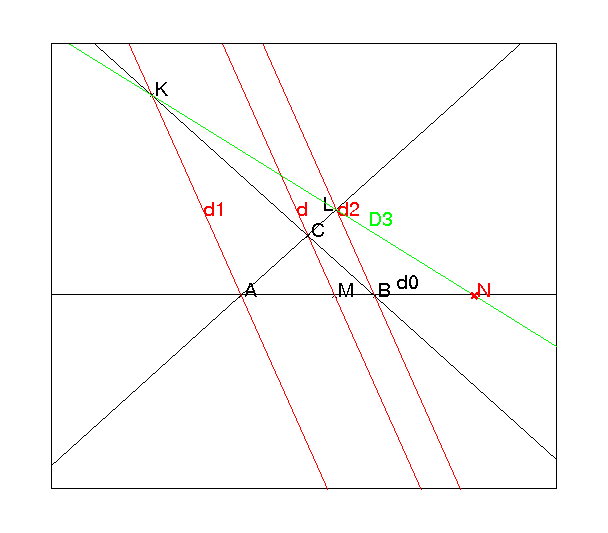
\includegraphics[width=10cm]{conj1}

{\bf Autre r\'eponse}\\
On d\'efinit 3 points $A,B,C$ non align\'es.\\
On d\'efinit les droites $d1=CA$, $d2=CB$, $d3=CM$.
On peut alors tracer la droite $d4$ pour que le faisceau $d1$, $d2$, $d3$, $d4$
soit harmonique.\\
On trace $D1$ la parall\`ele \`a la droite $d1$ passant par $B$ qui coupe $CM$ 
en $K$. On d\'efinit $L$ sur $D1$ tel que $BK=BL$ et $L \neq K$.\\
On trace $CL$ qui coupe $AB$ en $N$.\\

\begin{verbatim}
A:=point(-2,-2);
B:=point(3,-2);
C:=point(0.13,-1);
d0:=droite(A,B):;d0;
t:=element(0..1,0.3);
M:=element(d0,t);
d3:=droite(C,M):;d3;
d1:=droite(C,A);
d2:=droite(C,B):;d2;
D1:=parallele(B,d1,affichage=1);
K:=inter(d3,D1)[0];
L:=inter(cercle(B,K-B),D1)[1];
d4:=droite(C,L,affichage=2);
N:=affichage(inter(d0,d4)[0],1+epaisseur_point_2);
\end{verbatim}

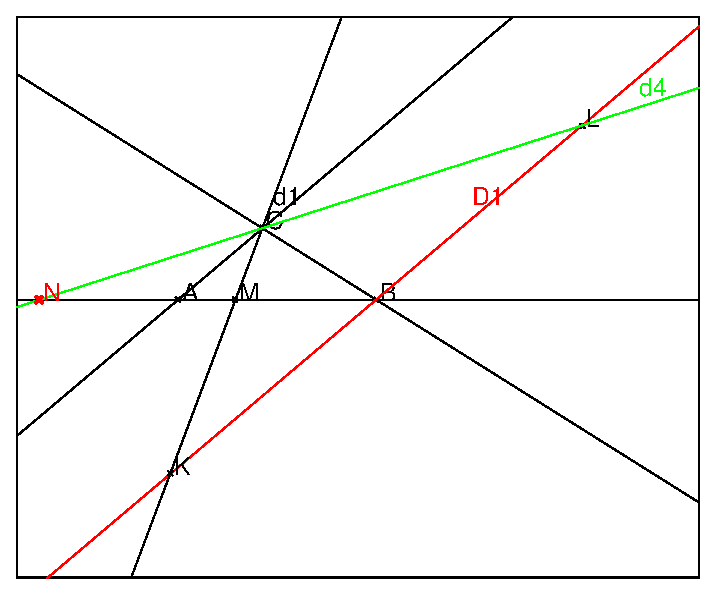
\includegraphics[width=10cm]{conj2}

\section{Polaires par rapport \`a deux droites}\index{polaire}\label{sec:polaire}
\subsection{D\'efinition}
Le lieu des conjugu\'es harmoniques d'un point $A$ par rapport \`a deux droites
$D1,D2$ est une droite $d$ v\'erifiant :
\begin{itemize}
\item si $D1$ et $D2$ sont concourantes en $O$, la droite $d$ passe par $O$ et 
le faisceau $(OA,d,D1,D2)$ est harmonique,
\item si $D1$ et $D2$ sont parall\'eles, la droite $d$ est parall\'ele \`a $D1$
et \`a $D2$, le faisceau $(d',d,D1,D2)$ est harmonique o\`u $d'$ est la 
parall\'ele \`a $D1$ passant par $A$.
\end{itemize}
\subsection{Un lieu}
Soient  un point $S$ et trois points $A,I,J$ align\'es.
Soit $M$ un point variable de la droite $SI$. La droite $AM$ coupe la droite 
$SJ$ en $N$.\\
On cherche le lieu de $K$ intersection de $IN$ et de $JM$ lorsque $M$ se 
d\'eplace sur la droite $SI$.
\subsubsection{Les figures}
On tape :
\begin{verbatim}
S:=point(1+5i,affichage=1);
A:=point(-4,affichage=1);
I:=point(0,affichage=1);
J:=point(7,affichage=1);
droite(A,J);
d:=droite(I,S,affichage=1);
droite(S,J,affichage=1);
t:=element((-2) .. 2,0.24,0.04)
M:=element(d,t);
N:=inter_droite(droite(A,M),droite(S,J),affichage=2);
droite(A,M,affichage=2);
segment(I,N);
segment(J,M);
K:=inter_droite(droite(I,N),droite(J,M),affichage=4);
L:=lieu(K,M):;
affichage(L,4+epaisseur_ligne_2);
B:=conj_harmonique(I,J,A);
droite(S,B);
\end{verbatim}

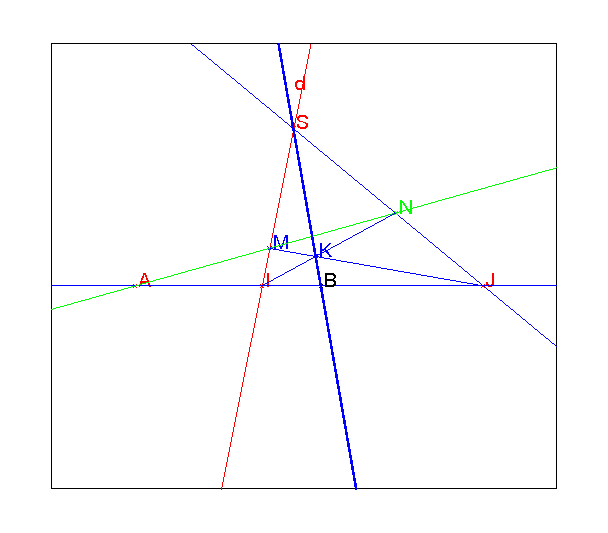
\includegraphics[width=10cm]{conj3}

On remarque que si $B$ est le conjugu\'e harmonique de $A$ par rapport \`a $I$ 
et $J$, le lieu $L$ de $K$ est la droite $SB$ . 

\subsubsection{La d\'emonstration}
Le lieu de $K$ est la polaire de $A$ par rapport \`a $CE$ et $FG$. En  effet
si $CE$ et $FG$ se coupent en $S$, si le point $L$ est le conjugu\'e 
harmonique de $A$ par rapport \`a $I$ et $J$ et si le point $P$ est le 
conjugu\'e harmonique de $A$ par rapport \`a $M$ et $N$, la polaire de $A$ par 
rapport \`a $CE$ et $FG$ passe par $S$, $L$ et $P$, et la polaire de $A$ par 
rapport \`a $IN$ et $JM$ passe par $K$, $L$ et $P$ donc, $K$ se trouve sur la 
polaire de $A$ par rapport \`a $CE$ et $FG$.

\section{P\^oles et polaires par rapport \`a un cercle ou une conique}\index{polaire}\label{sec:polairec}\label{sec:polec}
\subsection{D\'efinitions et propri\'et\'es}
On dit que 2 points $A$ et $B$ sont conjugu\'es par rapport \`a  un cercle 
ou une conique ($C$) si ils forment une division harmonique avec les points $E$
et $F$ o\`u la droite $AB$ coupe ($C$).\\ 
Le lieu des conjugu\'es harmoniques d'un point $A$ par rapport \`a  un cercle 
ou une conique $C$ est une droite $d$ appel\'ee {\bf polaire} de $A$ par 
rapport \`a ($C$). Si la polaire $d$ coupe ($C$) en $T_1$ et $T_2$ alors les 
droites $AT_1$ et $AT_2$ sont tangentes \`a  ($C$).\\
Lorsque ($C$) est un cercle ou une conique propre \`a toute droite $d$ on peut
faire correspondre un point $A$ qui admet $d$ comme polaire  par rapport \`a 
($C$) : on dit que $A$ est le {\bf p\^ole} de $d$.\\
Si la conique est d\'eg\'en\'er\'ee en deux droites $OU$ et $OV$ chaque droite 
passant par $O$ est la polaire d'une infinit\'e de points align\'es avec $O$
(cf \ref{sec:polaire}).

\subsection{Comment trouver l'\'equation de la polaire}
On va travailler en coordonn\`ees homog\`enes en dimension 2 : \\
un point $M(x,y)$ a pour coordonn\`ees homog\`enes $X,Y,T$ avec 
$x=X/T$ et $y=Y/T$.\\
Si l'\'equation de la conique est : 
$F(X,Y,T)=0$ alors $F$ est une forme quadratique de matrice $Q$ et on a, 
si $M=[X,Y,T]$ :
$$F(X,Y,T)=M*Q*M=0$$
La polaire du point $A=[X_a,Y_a,T_a]$ a pour \'equation :
$$X*F_X'(X_a,Y_a,T_a)+Y*F_Y'(X_a,Y_a,T_a)+T*F_T'(X_a,Y_a,T_a)=0$$
ou encore :
$$X_a*F_X'(X,Y,T)+Y_a*F_Y'(X,Y,T)+T_a*F_T'(X,Y,T)=0$$
ou encore :
$$M*Q*A=0$$

\subsection{Comment trouver les coordonn\'ees du p\^ole}
{\bf D\'efinitions} \\
Une droite $d$ d'\'equation $ux+vy+h=0$ a pour coordonn\'ees tangentielles
$u,v,h$.\\
L'\'equation tangentielle d'une courbe ($C$) est la 
condition n\'ecessaire et suffisante pour que la droite $d$ de coordonn\'ees 
tangentielles $[u,v,h]$ lui soit tangente.\\ 
{\bf \'Equation tangentielle de la conique ($C$)}\\
L'\'equation tangentielle de la conique ($C$) d'\'equation 
$F(X,Y,T)=M*Q*M=0$ est :
$$G(u,v,h)=[u,v,h]*inv(Q)*[u,v,h]$$
{\bf \'Equation tangentielle de la polaire}
L'\'equation tangentielle de la polaire de $A=[X_a,Y_a,T_a]$ par rapport \`a la
conique ($C$) est : $A*Q$.\\
{\bf Coordonn\'ees du p\^ole}\\
Soit $d$ une droite de coordonn\'ees tangentielles $u_d,v_d,h_d$ (donc 
d'\'equation $ux+vy+h=0$), le p\^ole de $d$ par rapport
\`a ($C$) a pour coordonn\'ees homog\`enes :
$$G_u'(u_d,v_d,h_d),G_v'(u_d,v_d,h_d)G_h'(u_d,v_d,h_d)$$
ou encore si $Q1=det(Q)*inv(Q)$
$$[u_d,v_d,h_d]*Q1$$

\subsection{Un exemple}
%voir expole.xws
Soient la conique $C$ d\'efinie par $x^2+2x*y+2*y^2-2*x=0$, la droite $d_b$
d'\'equation $x+3y-1=0$ et $A$ le point $2+i$.\\
Trouver la polaire $d_a$ de $A$ par rapport \`a $C$ etle p\^ole $B$ de $d_b$ 
par rapport \`a $C$.\\
On tape :\\
{\tt q1:=x\verb|^|2+2*x*y+2*y\verb|^|2-2*x}\\
{\tt q:=numer(subst(q1,[x,y]=[X/T,Y/T]))}\\
On obtient :\\
{\tt X\verb|^|2-2*X*T+2*X*Y+2*Y\verb|^|2}\\
On tape :\\
{\tt Q:=q2a(q,[X,Y,T])}\\
On obtient :\\
{\tt [[1,1,-1],[1,2,0],[-1,0,0]]}\\
On tape :\\
{\tt Q1:=det(Q)*inv(Q)}\\
On obtient :\\
{\tt [[0,0,2],[0,-1,-1],[2,-1,1]]}\\
On tape :\\
{\tt M:=[X,Y,T]}\\
{\tt U:=[u,v,h]}\\
{\tt A:=[2,1,1]}\\
{\tt da:=A*Q*M}\\
On obtient :\\
{\tt 2*X+4*Y-2*T}\\
La polaire $d_a$ de $A$ par rapport \`a $C$ a donc pour \'equation :
$x+2y-1=0$.\\
On tape :\\
{\tt A*Q}\\
On obtient :\\
{\tt [2,4,-2]}\\
La polaire $d_a$ de $A$ par rapport \`a $C$ a donc pour \'equation tangentielle
[2,4,-2] c'est \`a dire pour \'equation $x+2y-1=0$.\\
On tape :\\
{\tt db:=[1,3,-1]}\\
{\tt B:=db*Q1}\\
On obtient :\\
{\tt [-2,-2,-2]}\\
Le p\^ole $B$ de $d_b$ par rapport \`a $C$ a donc pour coordonn\'ees : 
$(1,1)$.\\
Pour avoir l'intersection $i_1$ et $i_2$ de $d_b$ avec $C$, on tape :\\
{\tt solve(normal(subst(x\verb|^|2+2*x*y+2*y\verb|^|2-2*x,x=1-3y))=0,y)} \\
On obtient :\\
{\tt [1/5*(-1-sqrt(6)),1/5*(-1+sqrt(6))]}\\
Les points d'intersection  $i_1$ et $i_2$ sont donc les points d'affixe $z_1$ 
et $z_2$ avec :\\
{\tt z1:=1+1/5*(-1-sqrt(6))*(-3+i), z2:=1+1/5*(-1+sqrt(6))*(-3+i)}\\
Pour avoir l'\'equation tangentielle de la conique $C$, on tape :\\
{\tt U:=[u,v,h]}\\
{\tt G:=normal(U*Q1*U)}\\
On obtient :\\
{\tt h\verb|^|2+4*h*u-2*h*v-v\verb|^|2}\\
On tape pour avoir l'\'equation tangentielle des tangentes \`a $C$ passant par $A$ (on choisit {\tt h=1}) :\\
{\tt normal(solve(subst([G=0,U*A=0],h=1),[u,v]))}\\
On obtient :\\
{\tt [[(-sqrt(3)+1)/2,sqrt(3)-2],[(sqrt(3)+1)/2,-sqrt(3)-2]]}\\
Les tangentes \`a $C$ passant par $A$ ont donc pour \'equation :\\
$(-\sqrt 3+1)x/2+(\sqrt 3-2)y+1=0$ et $(\sqrt 3+1)x/2-(\sqrt 3+2)y+1=0$\\
On tape :\\
{\tt plotimplicit(q1,[x,y]);a:=point(2+i);b:=point(1+i);}\\
{\tt t1:=droite((1-sqrt(3))/2*x+y*(-2+sqrt(3))+1=0,affichage=1);}\\
{\tt t2:=droite((1+sqrt(3))/2*x-y*(2+sqrt(3))+1=0,affichage=1);}\\
{\tt db:=droite(x+3y-1=0);da:=droite(x+2y-1=0);}\\
{\tt segment(z1,b,affichage=4);segment(z2,b,affichage=4);}\\
{\tt si1:=point(z1,affichage=4);i2:=point(z2,affichage=4);}\\
On obtient :\\

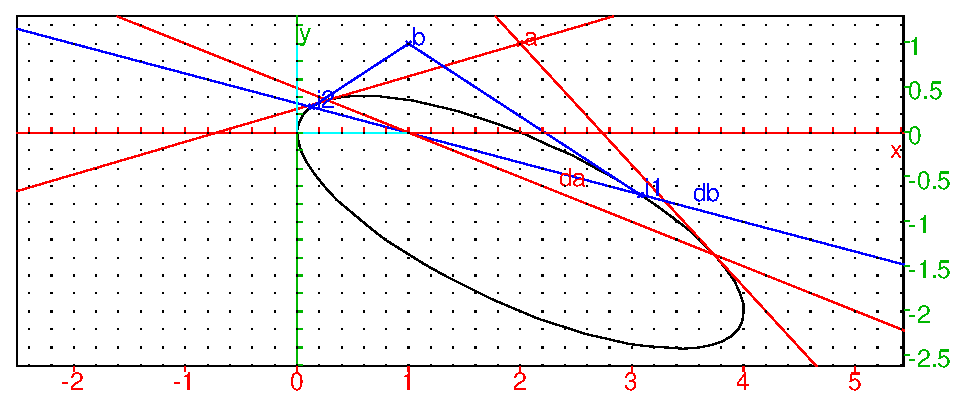
\includegraphics[width=12cm]{expole1}

\section{P\^oles et polaires par rapport \`a une sph\`ere ou une quadrique}\index{polaire}\label{sec:polaireq}\label{sec:poleq}
\subsection{D\'efinitions et propri\'et\'es}
On dit que 2 points $A$ et $B$ sont conjugu\'es par rapport \`a  une sph\`ere ou
une quadrique ($S$) si ils forment une division harmonique avec les points $E$
et $F$ o\`u la droite $AB$ coupe ($S$).\\ 
Le lieu des conjugu\'es harmoniques d'un point $A$ par rapport \`a  une sph\`ere
ou une quadrique ($S$) est un plan $P$ appel\'ee {\bf plan polaire} de $A$ par 
rapport \`a ($S$). Si le plan polaire $P$ coupe ($S$) en la courbe $T$ alors 
les droites joignant $A$ \`a un point de $T$ forment un c\^one  tangent 
\`a  ($S$).\\
Lorsque ($S$) est une sph\`ere ou une quadrique propre, \`a tout plan $P$ on
peut faire correspondre un point $A$ qui admet $P$ comme polaire  par rapport 
\`a ($S$) : on dit que $A$ est le {\bf p\^ole} de $P$.


\subsection{Comment trouver l'\'equation de la polaire}
On va travailler en coordonn\`ees homog\`enes : \\
en dimension 3 : $X,Y,Z,T$ avec $x=X/T$, $y=Y/T$ et $z=Z/T$.\\
Si l'\'equation de la quadrique est : 
$F(X,Y,Z,T)=0$ alors $F$ est une forme quadratique de matrice $Q$ et on a, 
si $M=[X,Y,Z,T]$ :
$$F(X,Y,Z,T)=M*Q*M=0$$
Le plan polaire du point $A=[X_a,Y_a,Z_a,T_a]$ a pour \'equation :
$$XF_X'(X_a,Y_a,Z_a,T_a)+YF_Y'(X_a,Y_a,Z_a,T_a)+ZF_Z'(X_a,Y_a,Z_a,T_a)+TF_T'(X_a,Y_a,Z_a,T_a)=0$$
ou encore :
$$X_aF_X'(X,Y,Z,T)+Y_aF_Y'(X,Y,Z,T)+Z_aF_Z'(X,Y,Z,T)+T_aF_T'(X,Y,Z,T)=0$$
ou encore :
$$M*Q*A=0$$
\subsection{Comment trouver les coordonn\'ees du p\^ole}
{\bf D\'efinitions}\\
Un plan $P$ d'\'equation $ux+vy+wz+h=0$ a pour coordonn\'ees tangentielles
$u,v,w,h$.\\ 
L'\'equation tangentielle d'une surface ($S$) est la 
condition n\'ecessaire et suffisante pour que le plan $P$ de coordonn\'ees 
tangentielles $[u,v,w,h]$ lui soit tangente.\\ 
{\bf \'Equation tangentielle de la quadrique ($S$)}\\
L'\'equation tangentielle de la conique ($S$) d'\'equation 
$F(X,Y,Z,T)=M*Q*M=0$ est :
$$G(u,v,w,h)=[u,v,w,h]*inv(Q)*[u,v,w,h]$$
{\bf \'Equation tangentielle du  plan polaire}
L'\'equation tangentielle du plan polaire de $A=[X_a,Y_a,Z_a,T_a]$ par rapport 
\`a la conique ($C$) est : $A*Q$.\\
{\bf Coordonn\'ees du p\^ole}\\
Soit $d$ une droite de coordonn\'ees tangentielles $u_d,v_d,w_d,h_d$ (donc 
d'\'equation $ux+vy+wz+h=0$), le p\^ole de $d$ par rapport
\`a ($C$) a pour coordonn\'ees homog\`enes :
$$G_u'(u_d,v_d,h_d),G_v'(u_d,v_d,h_d),G_h'(u_d,v_d,h_d)$$
ou encore si $Q1=det(Q)*inv(Q)$
$$[u_d,v_d,w_dh_d]*Q1$$

\subsection{Un exemple}
Soient la quadrique $S$ d\'efinie par $x^2+2x*y+2*y^2-2*x-2y+z^2=0$, $A$ le 
point $[2,-1,1]$, le plan $P_b$ d'\'equation $x+2y+z-2=0$ et le plan 
$P_c$ d'\'equation $x+3y+z-1=0$.\\
Trouver la polaire $d_a$ de $A$ par rapport \`a $S$, le p\^ole $B$ 
de $d_b$ par rapport \`a $S$ et le p\^ole $C$ de $d_c$ par rapport \`a $S$.\\
On tape :\\
{\tt q1:=x\verb|^|2+2x*y+2*y\verb|^|2-2*x-2y+z\verb|^|2}\\
{\tt q:=numer(subst(q1,[x,y,z]=[X/T,Y/T,Z/T]))}\\
On obtient :\\
{\tt X\verb|^|2-2*X*T+2*X*Y-2*Y*T+2*Y\verb|^|2+Z\verb|^|2}\\
On tape :\\
{\tt Q:=q2a(q,[X,Y,Z,T])}\\
On obtient :\\
{\tt [[1,1,0,-1],[1,2,0,-1],[0,0,1,0],[-1,-1,0,0]]}\\
On tape :\\
{\tt Q1:=det(Q)*inv(Q)}\\
On obtient :\\
{\tt [[-1,1,0,1],[1,-1,0,0],[0,0,-1,0],[1,0,0,1]]]}\\
On tape :\\
{\tt M:=[X,Y,T]}\\
{\tt U:=[u,v,h]}\\
{\tt A:=[2,-1,1,1]}\\
{\tt Pa:=A*Q*M}\\
On obtient :\\
{\tt -Y+Z-T}\\
Le plan polaire $d_a$ de $A$ par rapport \`a $S$ a donc pour \'equation :
$-y+z-1=0$\\
On tape :\\
{\tt A*Q}\\
On obtient :\\
{\tt [0,-1,1,-1]}\\
Le plan polaire $P_a$ de $A$ par rapport \`a $S$ a pour \'equation 
tangentielle [0,-1,1,-1] c'est \`a dire pour \'equation $-y+z-1=0$\\
On tape :\\
{\tt Pb:=[1,2,1,-2]}\\
{\tt B:=Pb*Q1}\\
On obtient :\\
{\tt [-1,-1,-1,-1]}\\
Le p\^ole $B$ de $d_b$ par rapport \`a $S$ est donc le point coordonn\'ees
[1,1,1].\\
On tape :\\
{\tt Pc:=[1,3,1,-1]}\\
{\tt C:=Pb*Q1}\\
On obtient :\\
{\tt [1,-2,-1,0]}\\
Le p\^ole $C$ de $d_c$ par rapport \`a $S$ se trouve \`a l'infini dans la 
direction  [1,-2,-1] car le plan $P_c$ passe par le centre de l'ellipsoide $S$
On tape :\\
{\tt normal(solve([Pa=0,qq=0,T=1],[X,Y,Z,T]))}\\
On obtient :\\
{\tt [[X,(-X+sqrt(-2*X\verb|^|2+6*X-3))/3,(-X+sqrt(-2*X\verb|^|2+6*X-3)+3)/3,1],}\\
{\tt  [X,(-X-sqrt(-2*X\verb|^|2+6*X-3))/3,(-X-sqrt(-2*X\verb|^|2+6*X-3)+3)/3,1]]}\\
On tape :\\
{\tt CC:=plotparam([X,(-X+sqrt(-2*X\verb|^|2+6*X-3))/3,}\\
{\tt (-X+sqrt(-2*X\verb|^|2+6*X-3)+3)/3],X)}\\
{\tt CC2:=plotparam([X,(-X-sqrt(-2*X\verb|^|2+6*X-3))/3,}\\
{\tt (-X-sqrt(-2*X\verb|^|2+6*X-3)+3)/3],X)}\\
Pour avoir le c\^one des tangentes de sommet {\tt a}, on tape :
\begin{verbatim}
conetan():={
local L,M,N,X;
L:=NULL;
a:=point([2,-1,1]);
pour X de 0.63 jusque 2.37 pas 0.1 faire
M:=point(X,(-X+sqrt(-2*X^2+6*X-3))/3,
   (-X+sqrt(-2*X^2+6*X-3)+3)/3);
N:=point(X,(-X-sqrt(-2*X^2+6*X-3))/3,
   (-X-sqrt(-2*X^2+6*X-3)+3)/3);
L:=L,droite(a,M),droite(a,N);
fpour;
retourne L;
}:;
\end{verbatim}
Dans un \'ecran de g\'eom\'etrie 3d on tape :\\
\begin{verbatim}
plotimplicit(q1,[x,y,z],affichage=rouge);
plan(-y+z-1=0,affichage=jaune);
affichage([CC,CC2],vert+epaisseur_ligne_7);
a:=point([2,-1,1]);
conetan();
\end{verbatim}
On obtient :

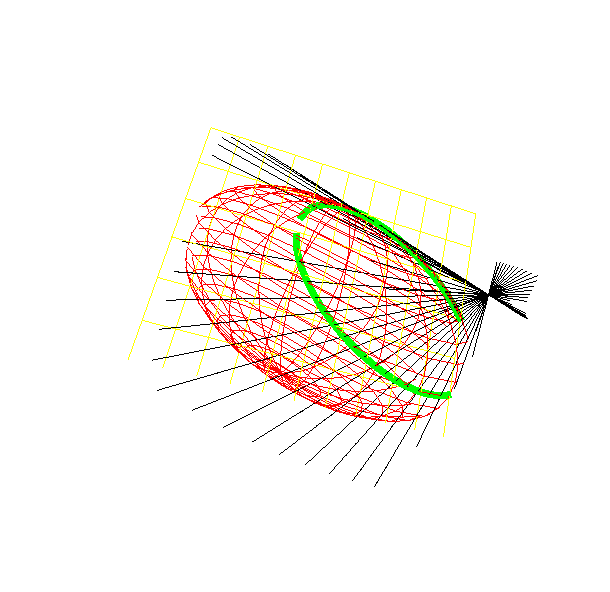
\includegraphics[width=\textwidth]{expole3}

\section{Les coniques}\index{ellipse}\index{hyperbole}\index{parabole}
\begin{itemize}
\item L'ellipse\\
{\tt ellipse(A,B,C)} trace l'ellipse de foyers {\tt A} et
{\tt B} passant par {\tt C}.\\
{\tt ellipse(A,B,a)} o\`u {\tt a} est un r\'eel, trace l'ellipse de 
foyers {\tt A} et
{\tt B} ayant {\tt a} comme demi-grand axe.
\item L'hyperbole\\
{\tt hyperbole(A,B,C)} trace l'hyperbole de foyers {\tt A} et
{\tt B} passant par {\tt C}.\\
{\tt hyperbole(A,B,a)} o\`u {\tt a} est un r\'eel,  trace l'hyperbole
 de foyers {\tt A} et {\tt B} ayant {\tt a} comme demi-grand axe.
\item La parabole\\
{\tt parabole(A,B)} trace la parabole de foyer {\tt A} et de sommet {\tt B}.
\end{itemize}
{\bf Activit\'e}\\
Tracer un cercle tangent \`a une droite et passant par deux points donn\'es.\\
Pour cela, cr\'eer quatre points {\tt A}, {\tt B}, {\tt C} et {\tt D}.\\
Tracer la droite {\tt E} passant par {\tt A} et {\tt B}.\\
Construire un cercle {\tt C1} passant par {\tt C} et {\tt D} tangent \`a la
droite {\tt E}.\\
{\bf R\'eponse}\\
On sait que le centre du cercle cherch\'e est sur la m\'ediatrice de $CD$ et
sur la parabole $P$ de foyer $C$ et de directrice la doite $AB$.\\
On clique avec la souris pour avoir quatre points {\tt A}, {\tt B}, {\tt C}
et {\tt D} puis on ex\'ecute la liste des instructions qui se trouve dans 
{\tt geo11} (faire {\tt Charger session} du 
menu {\tt Fich} de {\tt Xcas} et selectionner {\tt geo11} du r\'ep\'ertoire 
{\tt examples/geo} pour ex\'ecuter ce fichier).\\
Voici le d\'etail de {\tt geo11} :\\
{\tt E:=droite(A,B)} \\
trace la droite $E$ passant par $A$ et $B$,\\
{\tt M:=mediatrice(C,D)}\\
 trace la m\'ediatrice de $CD$,\\ 
{\tt H:=projection(E,C)}\\
 d\'efinit la projection orthogonale de $C$ sur $E$,\\
{\tt P:=parabole(C,milieu(C,H)))} \\
trace la parabole de foyer $C$ et de directrice $E$,\\
{\tt N:=inter(P,M)}\\
$N$ est la liste des points d'intersection de la droite $M$ et de la parabole $P$,\\
{\tt C1:=cercle(N[0],C-N[0])}\\
trace le cercle de centre {\tt N[0]} passant par {\tt C} : il repond \`a la question.\\ 
{\tt C2:=cercle(N[1],C-N[1])} trace le cercle de centre {\tt N[1]} passant par {\tt C} : il repond \`a la question.\\
{\tt Q:=parabole(D,milieu(D,projection(E,D)))} trace la parabole de foyer $D$ 
et de directrice $E$, elle passe par $N$. Cela prouve qu'il n'y a pas d'autres
solutions.\\ 
\chapter{Le th\'eor\`eme de Pythagore}
\section{Le th\'eor\`eme}
Dans un triangle rectangle, le carr\'e de l'hypot\'enuse est la somme des 
carr\'es des deux autres c\^ot\'es.
\section{Une d\'emonstration qui saute aux yeux}
On consid\`ere un triangle rectangle $T$ de co\'es $a,b,c$ ($c$ est 
l'hypot\'enuse et on suppose $a\geq b$), on veut donc montrer que $a^2+b^2=c^2$.\\
On  fait quatre copies de ce triangle $T$ et deux copies $C_1$ et $C_2$
d'un carr\'e de cot\'es $a+b$. On dispose les quatres copies du triangle dans 
les carr\'es $C_1$ et $C_2$ selon la figure ci-dessous :\\

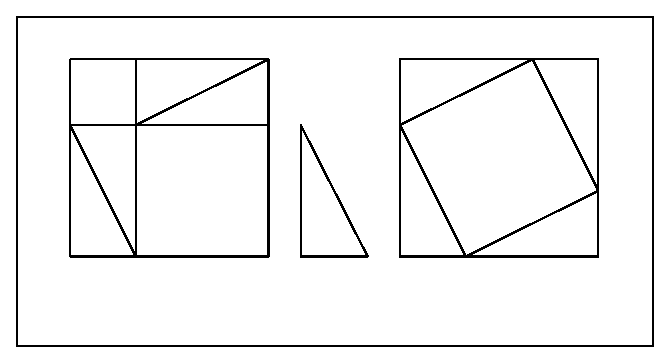
\includegraphics[width=\textwidth]{pytha1}

Dans le carr\'e $C_1$ on a 4 triangles $T$ et deux carr\'es l'un de cot\'es $a$
(de surface $a^2$)  et l'autre de cot\'es $b$ (de surface $b^2$).\\
Dans le carr\'e $C_2$ on a 4 triangles $T$ et un carr\'e  de cot\'es $c$
(de surface $c^2$).\\
Comme les surfaces de $C_1$ et de $C_2$ sont les m\^emes on en d\'eduit que :\\
$a^2+b^2=c^2$.
\begin{verbatim}
carre(-4-i,-1-i);
carre(1-i,4-i);
triangle_rectangle(-0.5-i,0.5-i,2);
segment(-3-i,-3+2*i);
segment(-4+i,-1+i);
segment(-3-i,-4+i);
segment(-3+i,-1+2*i);
segment(1+i,2-i);
segment(1+i,3+2*i);
segment(4,3+2*i);
segment(4,2-i);
\end{verbatim}
\section{Le th\'eor\`eme et la formule $(a+b)^2=a^2+2ab+b^2$}
On ne dessine que le carr\'e $C_2$ et on a :\\
$C_2$ a comme  surface $(a+b)^2$ \\
les quatres triangles $T$ ont comme  surface $2ab$ \\
Le carr\'e central a comme  surface $c^2$ et aussi  $(a+b)^2-2ab$\\
Donc :\\
$(a+b)^2-2ab=c^2$\\
On sait que $(a+b)^2=a^2+2ab+b^2$ (identit\'e remarquable) donc\\
$c^2=a^2+b^2$
\section{Le th\'eor\`eme et la formule $(a-b)^2=a^2-2ab+b^2$}
On consid\`ere un carr\'e $C$ de cot\'e $c$ et on place les quatres copies du 
triangles rectangle $T$ selon la figure ci-dessous : 
\begin{verbatim}
triangle_rectangle(0,1,2);
triangle_rectangle(i,2*i,2);
triangle_rectangle(-1+i,-2+i,2);
triangle_rectangle(-1,-1-i,2);
\end{verbatim}

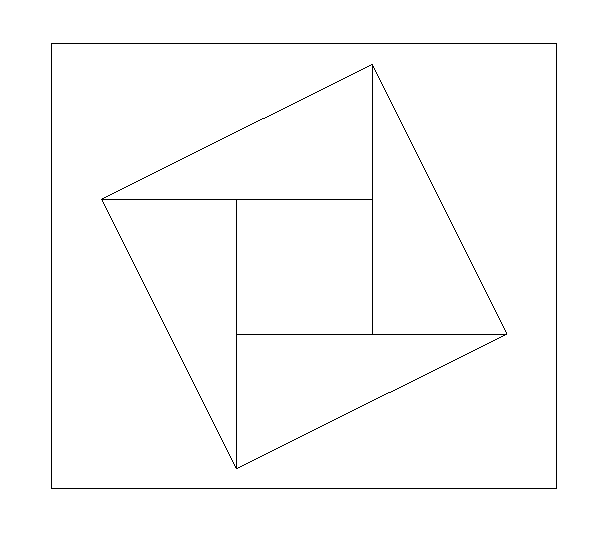
\includegraphics[width=6cm]{pytha2}\\

Le carr\'e de cot\'e $c$ est compos\'e d'un carr\'e de cot\'es $a-b$ et
 de 4  triangles $T$ donc on a :\\
$(a-b)^2+2ab=c^2$\\
On sait que $(a-b)^2=a^2-2ab+b^2$ (identit\'e remarquable) donc\\
$c^2=a^2+b^2$.
\section{Le th\'eor\`eme et un puzzle}
Soit une forme constitu\'ee de deux carr\'es de cot\'es $a$ et $b$ (avec 
$a\geq b$) dispos\'es selon la figure :\\

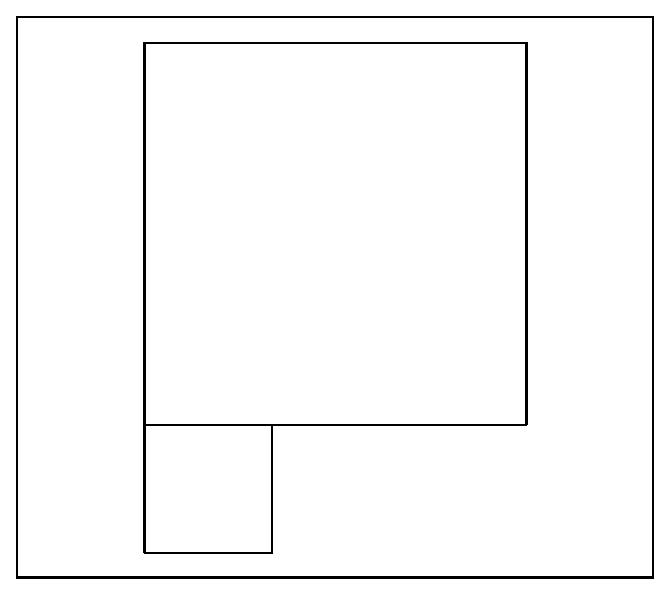
\includegraphics[width=6cm]{pytha3}\\

Comment d\'ecouper cette forme pour faire un puzzle de trois pi\`eces 
permettant de reconstituer un carr\'e ?\\
{\bf Solution}\\
Si le carr\'e de c\^ot\'es $a$ a pour sommets 
$(0,a,a(1+i),ia)$, on joint les points $i(a-b)$ et $a(1+i)$ ainsi que les 
points $i(a-b)$ et $b(1-i)$.\\ 
On obtient :\\

 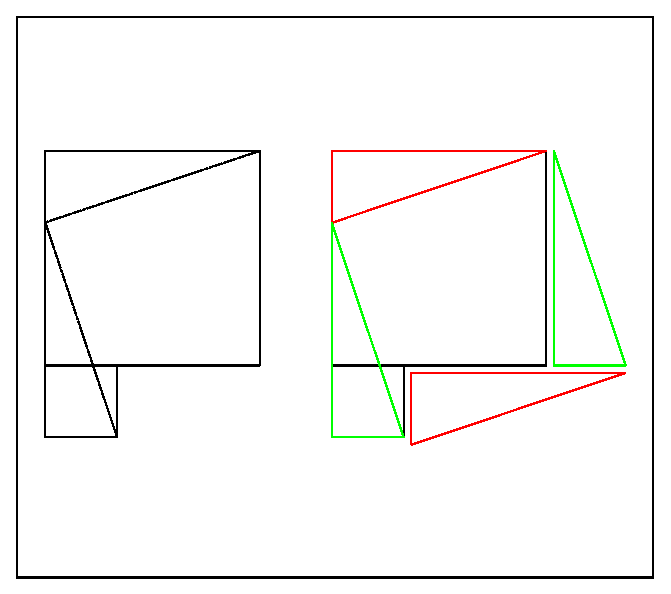
\includegraphics[width=10cm]{pytha4}\\

On tape pour avoir cette figure :
\begin{verbatim}
carre(-4-i,-1-i);
carre(-4-2*i,-3-2*i);
segment(-3-2*i,-4+i,affichage=ligne_tiret);
segment(-1+2*i,-4+i,affichage=ligne_tiret);
carre(-i,3-i);
carre(-2*i,1-2*i);
couleur(triangle_rectangle(2*i,i,3),rouge);
couleur(triangle_rectangle(1.1-1.1*i,1.1-2.1*i,3),rouge)
couleur(triangle_rectangle(-2*i,1-2*i,3),vert);
couleur(triangle_rectangle(3.1-i,4.1-i,3),vert)
\end{verbatim}

On peut simuler un vrai puzzle en d\'epla\c{c}ant avec la souris les trois 
pi\`eces.\\
On tape :  
\begin{verbatim}
A:=point(-4,-1);
B:=point(-1,-1);
carre(A,B,C,D);
E:=element(droite(A,B),0.3);
carre(E,A,F,G);
H:=F+C-B;
segment(H,C);
segment(H,G);
P:=polygone(C,H,G,E,B);
T1:=triangle(H,G,F);
T2:=triangle(H,C,D);
\end{verbatim}
Puis on bouge le polyg\^one et les 2 triangles pour faire 1 grand carr\'e : 
pour cela on se met en mode {\tt Pointeur} et on clique sur le c\^ot\'e $EB$ du
polyg\^one et on le d\'eplace. Puis
on clique sur le c\^ot\'e $HC$ du triangle($H,C,D$) et on le d\'eplace pour 
amener $D$ en $E$, puis on clique sur le c\^ot\'e $HG$ du triangle($H,G,F$) et 
on le d\'eplace pour amener $F$ en $B$.\\
{\bf Remarque} : on peut tracer les segments $HC$ et $HG$ seulement apres avoir
d\'eplac\'e le polyg\^one et les 2 triangles.\\
On obtient :\\

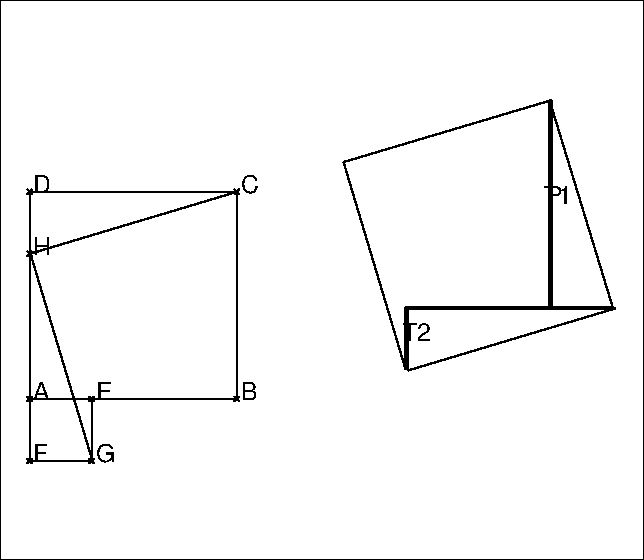
\includegraphics[width=10cm]{pytha5}\\

\section{Le th\'eor\`eme et un autre puzzle}
On dispose de deux carr\'es de c\^ot\'es $a$ et $b$ ($a\geq b$).\\
Comment d\'ecouper le carr\'e de c\^ot\'es $a$ en quatre morceaux pour pouvoir 
faire, avec ces 4 morceaux et le carr\'e de cot\'e $b$, un puzzle de cinq
pi\`eces permettant de reconstituer un carr\'e ?\\
{\bf Une solution}\\
On pose $a-b=2d$ et si le carr\'e de c\^ot\'e $a$ a pour sommets 
$(0,a,a(1+i),ia)$, on joint les points $id$ et $a+i(d+b)$ ainsi que les points 
$d+b$ et $d+ia$. Ces deux segments ont pour longueur $c=\sqrt{a^2+b^2}$, et se 
coupent selon quatre angles droits qui deviendront les sommets du carr\'e 
solution de c\^ot\'es $c=\sqrt{a^2+b^2}$.\\
On obtient le d\'ecoupage du carr\'e de c\^ot\'e $a$ et le carr\'e constitu\'e 
des 5 pi\`eces dans la figure ci-dessous : \\

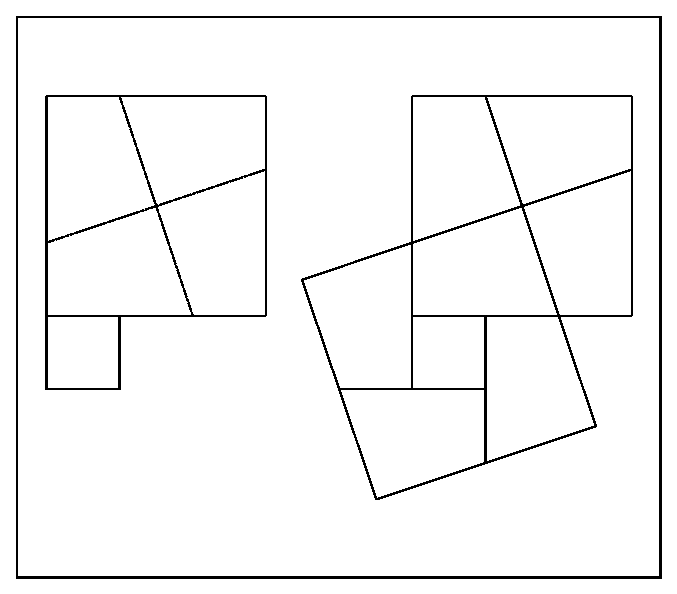
\includegraphics[width=6cm]{pytha6}\\

Pour faire cette figure on tape :
\begin{verbatim}
carre(-5-2i,-4-2i);
carre(-5-i,-2-i);
segment(-5,-2+i,affichage=ligne_tiret);
segment(-3-i,-4+2i,affichage=ligne_tiret);
carre(-i,3-i);
segment(1+2*i,2-i)
segment(0,3+i)
carre(-2*i,1-2*i);
segment(2-i,2.5-2.5*(i));
segment(1-2*i,1-3*(i));
segment(2.5-2.5*(i),-0.5-3.5*(i));
segment(1-2*(i),-1-2*(i));
segment(-1.5-0.5*i,0);
segment(-1.5-0.5*i,-1-2*i);
segment(-0.5-3.5*(i),-1-2*(i));
\end{verbatim}
On peut simuler un vrai puzzle en d\'epla\c{c}ant avec la souris les cinq
pi\`eces.\\
On tape :  
\begin{verbatim}
A:=point(-4,-1);
B:=point(-1,-1);
carre(A,B,C,D):;
E:=element(droite(A,B),0.3);
carre(E,A,F,G):;
I:=milieu(E,B);
J:=D+B-I;
K:=rotation(A,pi/2,A+B-I);
L:=C+A-K;
segment(I,J);
segment(K,L);
M:=inter(droite(I,J),droite(K,L))[0];
quadrilatere(D,J,M,K);
quadrilatere(C,J,M,L);
quadrilatere(A,I,M,K);
quadrilatere(B,I,M,L);
quadrilatere(E,A,F,G);
\end{verbatim}
Puis on bouge les 5 quadrilat\`eres dans un grand carre : pour cela, on se met 
en mode pointeur et pour faciliter la s\'election des quadrilat\`eresn on prend
soin de ne pas dessiner le {\tt carre(A,B,C,D):;}
gr\^ace au  {\tt :;}. On clique successivement sur un c\^ot\'e de chaque 
quadrilat\`ere et on les d\'eplace. Puis on dessine le {\tt carre(A,B,C,D)}
en enlevant le {\tt :} \\
On obtient :\\

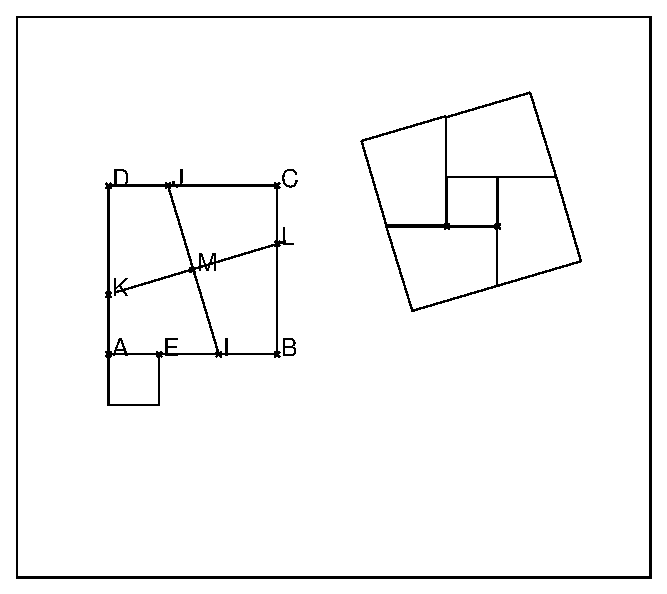
\includegraphics[width=10cm]{pytha7}\\ 

{\bf Exercice : autre d\'ecoupage}\\ 
 Trouver d'autres solutions.\\
On peut en effet d\'ecouper le carre $ABCD$ selon n'importe quelle parall\`ele
\`a $IJ$ et $KL$...\`a vous de la montrer !

\section{La formule $(a-b)^2=a^2-2ab+b^2$ comme exercice}
Soit $ABC$ est un triangle quelconque et $L$ le pied de la hauteur issue 
de $C$. On pose $AB=c$, $AC=b$,  $BC=a$, $CH=h$, $HB=d_1$, $HA=d_2$.
Montrer que :
$h^2=b^2-d_2^2$,\\
$h^2=a^2-d_1^2$,\\
$d_2=b\cos(A)$, \\
en d\'eduire que: $a^2=d_1^2+h^2=d_1^2-d_2^2+b^2$.\\
En observant la figure, montrer que :\\
la surface verte $V$ = $a^2$\\
la surface jaune $J$= $b^2$\\ 
la surface rouge $R$=$d_1^2-d_2^2$\\

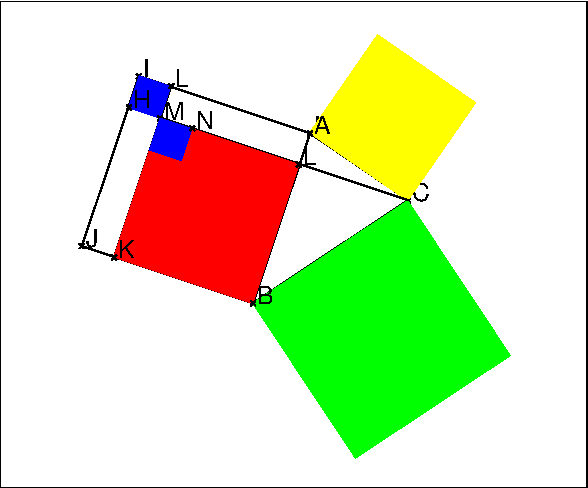
\includegraphics[width=\textwidth]{pytha8}\\

Que vaut la surface rouge $R$ par rapport \`a $c$ et $d_2$, 
par rapport \`a $b,c,\cos(A)$  ?
En d\'eduire la g\'en\'eralistion du th\'eor\`eme de Pythagore.\\
{\bf Solution}
On applique le th\'eor\`eme de Pythagore aux triangles rectangles
$ALC$ et $BLC$ donc :\\
$h^2=b^2-d_2^2$ et\\
$h^2=a^2-d_1^2$,\\
On a donc :
$V=R+J=a^2=d_1^2-d_2^2+b^2$\\
Puisque $c=d_1+d_2$ on a $d_1-d_2=c-2d_2=c-2b\cos(A)$:\\
$R=d_1^2-d_2^2=c(c-2d_2)=c(c-2b\cos(A))=c^2-2bc\cos(A)$\\
$c^2=R+2d_2^2+2d_1d_2=R+2c*d_2=a^2-b^2+2bc\cos(A)$ \\
Donc\\
$a^2=b^2+c^2-2bc\cos(A)$


\chapter{Le th\'eor\`eme de 1968}
\section{Le th\'eor\`eme}
Soit un triangle quelconque $ABC$.
On construit sur les c\^ot\'es du triangle $ABC$ les carr\'es directs
$CBDE$, $ACGF$ et $BAKH$, puis les parall\'elogrammes $DBHJ$ et $GCEL$.\\

\begin{center}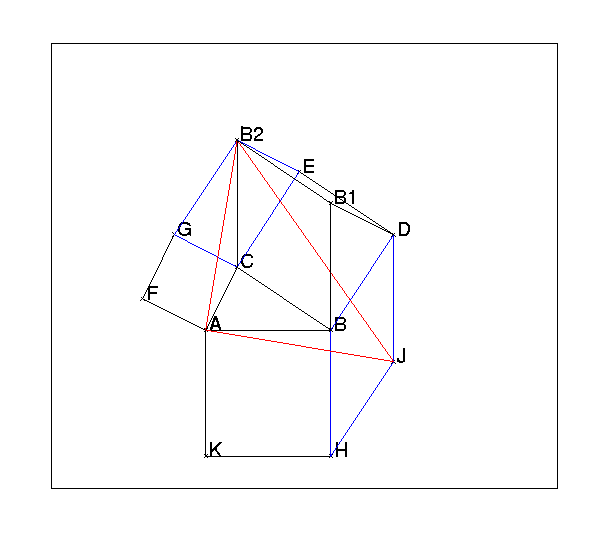
\includegraphics[width=8cm]{th1968d}\end{center}

{\bf Remarque} : si  $ABC$ est direct les carr\'es sont \`a l'ext\'erieur du 
triangle.\\
On a la propri\'et\'e suivante :
Le triangle $AJL$ est isoc\`ele rectangle direct.

\section{La figure}
Pour faire la figure, on tape  les instructions suivantes qui se trouvent 
dans le fichier 
{\tt th1968.xws} : 
\begin{verbatim}
A:=point(-4,-1);
B:=point(-2,-1);
C:=point(-3.5,0);
triangle(A,B,C);
carre(B,A,K,H);
carre(C,B,D,E);
carre(A,C,G,F);
J:=H+D-B;
polygone(D,B,H,J,affichage=bleu);
L:=E+G-C:;legend(L,"L",quadrant2;
polygone(C,G,L,E,affichage=bleu);
triangle(A,J,L,affichage=rouge);
\end{verbatim}

\section{Une d\'emonstration g\'eom\'etrique}
On suppose que le triangle $ABC$ est direct car la figure est plus lisible.\\
On fait des constructions suppl\'ementaires et on tape :
\begin{verbatim}
B1:=translation(B-H,B);
B2:=translation(C-B,B1);
segment(B1,B);
segment(B1,L);
segment(B1,D);
segment(C,L);
\end{verbatim}
\begin{center}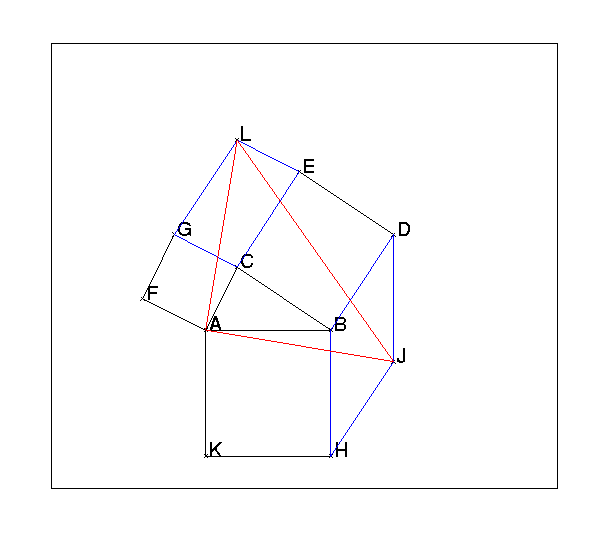
\includegraphics[width=10cm]{th1968}\end{center}

On remarque que {\tt B2} est confondu avec {\tt L} puisque
les triangles {\tt B1BD} et {\tt LCE} sont \'egaux au triangle 
{\tt ABC} en effet :\\
- le triangle {\tt B1BD} est le transform\'e du triangle {\tt ABC}
par rotation de centre {\tt B} et d'angle {\tt -pi/2}, et \\
- le triangle {\tt LCE} est le transform\'e du triangle {\tt ABC}
par la composition de la rotation de centre {\tt C} et d'angle {\tt -pi/2} 
et de la translation de vecteur {\tt E-C}.\\
La rotation de centre  {\tt A} et d'angle  {\tt pi/2} transforme
{\tt H} en {\tt B1} et  {\tt HJ} en {\tt B1B2}.\\
Donc la rotation de centre  {\tt A} et d'angle  {\tt pi/2} transforme {\tt J} en {\tt B2}.\\
Donc, puisque {\tt B2} est confondu avec {\tt L}, la rotation de centre  
{\tt A} et d'angle {\tt pi/2} transforme {\tt J} en {\tt L}\\
Donc le triangle {\tt AJL} est isoc\`ele rectangle direct.

\section{Une d\'emonstration avec les complexes}
Soit {\tt a=affixe(A), b=affixe(B), c=affixe(C)}\\
On a :\\
{\tt j=affixe(J)=b+i*(a-b)-i*(c-b)=b+i(a-c)}\\
{\tt l=affixe(L)=c+i*(b-c)-i*(a-c)=c+i(b-a)}\\
On a donc :
$$ l-a=c-a+i*(b-a)=i^2*(a-c)+i*(b-a)=i*(b-a+i(a-c))=i*(j-a)$$
L'\'egalit\'e {\tt l-a=i*(j-a)} prouve que {\tt L} se d\'eduit de {\tt J}
par la rotation de centre {\tt A} et d'angle {\tt pi/2}.
\section{La d\'emonstration du th\'eor\`eme avec {\tt Xcas}}
On suppose que le point {\tt A} est \`a l'origine du rep\`ere et que 
le point {\tt B} est le point d'affixe 2.
Le point {\tt C} a comme affixe $a+ib$, avec $a$ et $b$ quelconques.\\
Pour faire la figure on suppose que $a=-1$ et que $b=-1$.\\
On tape les instructions suivantes qui se trouvent dans le fichier 
{\tt th1968d.xws} :
\begin{verbatim}
assume(a=-3.5);
assume(b=0);
A:=point(-4,-1);
B:=point(-2,-1);
C:=point(a,b);
T1:=couleur(carre(B,A,K,H),vert);
T2:=couleur(carre(C,B,D,E),vert);
T3:=couleur(carre(A,C,G,F),vert);
J:=H+(D-B); 
P1:=couleur(polygone(D,B,H,J),rouge);
L:=E+(G-C);
P2:=couleur(polygone(L,E,C,G),rouge);
p:=normal((affixe(J)-affixe(A))/(affixe(L)-affixe(A)));
normal(longueur2(A,L)-longueur2(A,J));
normal(angle(A,J,L));
\end{verbatim}
On obtient {\tt -i}, {\tt 0} et {\tt pi/2} comme r\'esultats des 3 derni\`eres 
commandes :
\begin{center}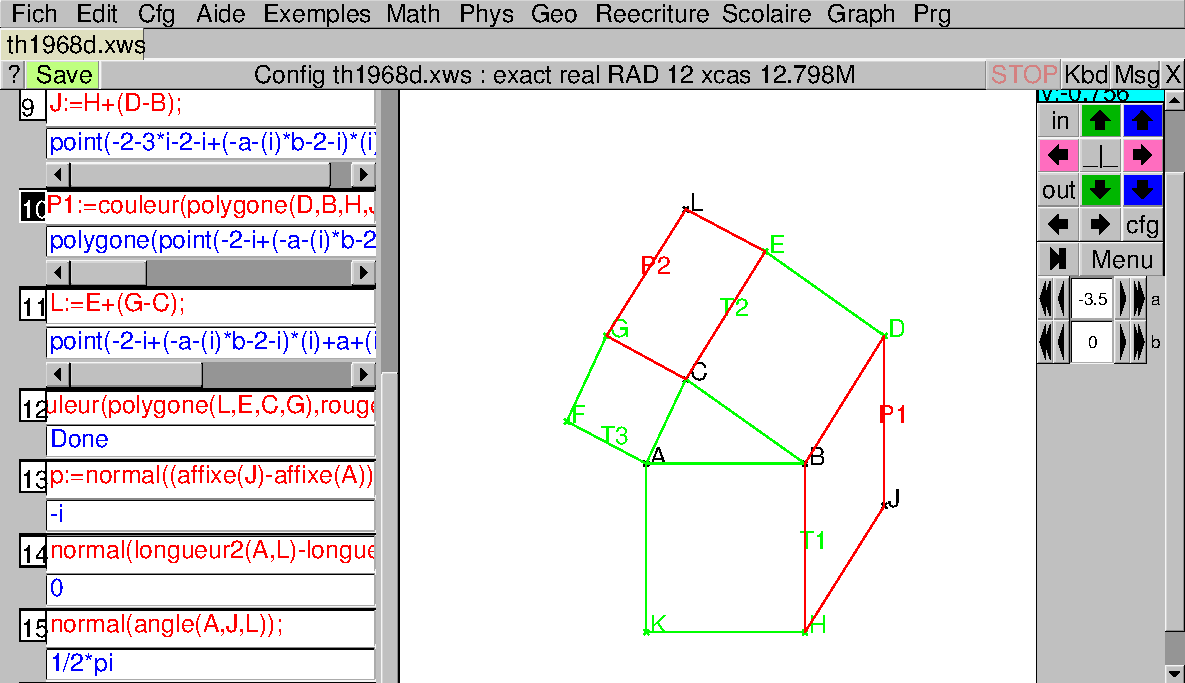
\includegraphics[width=\textwidth]{th1968w}\end{center}

\chapter{Le th\'eor\`eme de Napol\'eon}
\section{Le th\'eor\`eme}
Soit un triangle quelconque $ABC$.\\
On construit \`a l'ext\'erieur du triangle $ABC$ les triangles \'equilat\`eraux
$BAD$, $CBE$ et $ACF$ qui ont pour centre de gravit\'e : $G1$, $G2$ et $G3$.\\
On a les propri\'et\'es suivantes :\\
Le triangle $G1G2G3$ est \'equilat\'eral et a m\^eme centre de gravit\'e que 
le triangle $ABC$.\\
Les droites $AE$, $DC$, $BF$ sont concourantes en un point $T$ qui s'appelle le
 point de Torricelli.\\
Le point $T$ est aussi le point de concours des cercles circonscrits aux 
triangles $BAD$, $CBE$ et $ACF$.


\section{La figure}

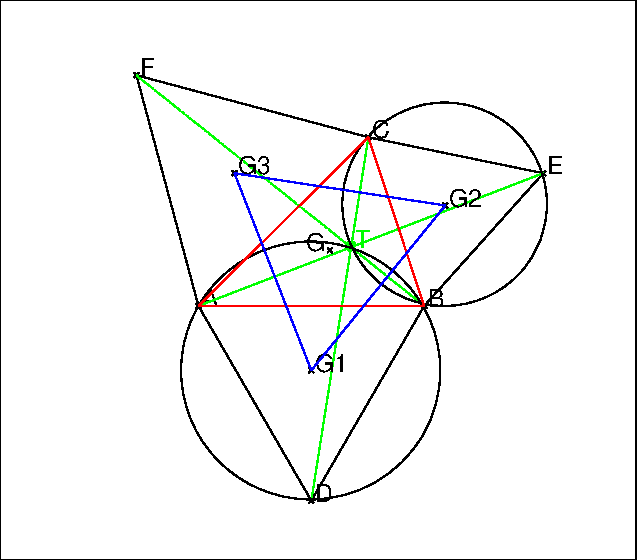
\includegraphics[width=8cm]{napo1}\\

Pour faire cette figure, on tape dans un \'editeur de programme : 
\begin{verbatim}
A:=point(-2.,-1.,'affichage'=0);
B:=point(2.,-1,'affichage'=0);
C:=point(1.,2,'affichage'=0);
triangle_equilateral(B,A,D);
triangle_equilateral(C,B,E);
triangle_equilateral(A,C,F);
segment(A,E,affichage=2);
segment(C,D,affichage=2);
segment(B,F,affichage=2+ligne_tiret);
T:=inter_droite(droite(A,E),droite(C,D),affichage=2+
                 epaisseur_point_2);
circonscrit(A,B,D);
circonscrit(C,B,E);
G1:=isobarycentre(A,B,D);
G2:=isobarycentre(C,B,E);
G3:=isobarycentre(A,C,F);
G:=isobarycentre(A,C,B,affichage=quadrant2);
triangle(A,B,C,affichage=1);
triangle(G1,G2,G3,affichage=4);
\end{verbatim}

\section{Les d\'emonstrations g\'eom\'etriques}
\subsection{Avec les cercles circonscrits \`a $BAD$, $CBE$ et $ACF$}
On trace les cercles $C_1$, $C_2$ et $C_3$ circonscrits aux triangles $ADB$, 
$BEC$ et $CFA$ de centres respectifs $G_1$, $G_2$ et $G_3$.\\
Pour faire la figure, on tape :
\begin{verbatim}
A:=point(-2.,-1.,'affichage'=0);
B:=point(2.,-1,'affichage'=0);
C:=point(1.,2,'affichage'=0);
D:=rotation(B,pi/3,A);
E:=rotation(C,pi/3,B);
F:=rotation(A,pi/3,C);
C1:=circonscrit(A,B,D,affichage=2);
C2:=circonscrit(C,B,E,affichage=2);
C3:=circonscrit(C,A,F,affichage=2+ligne_tiret);
G1:=isobarycentre(A,B,D);
G2:=isobarycentre(C,B,E);
G3:=isobarycentre(A,C,F);
G:=isobarycentre(A,C,B,affichage=quadrant2);
triangle(A,B,C,affichage=1);
triangle(G1,G2,G3,affichage=4);
T:=inter(C1,C2,affichage=2+epaisseur_point_2)[1];
angle(D,B,A,"");
angle(T,B,A,"");
angle(T,C,B,"");
angle(E,C,B,"");
\end{verbatim}

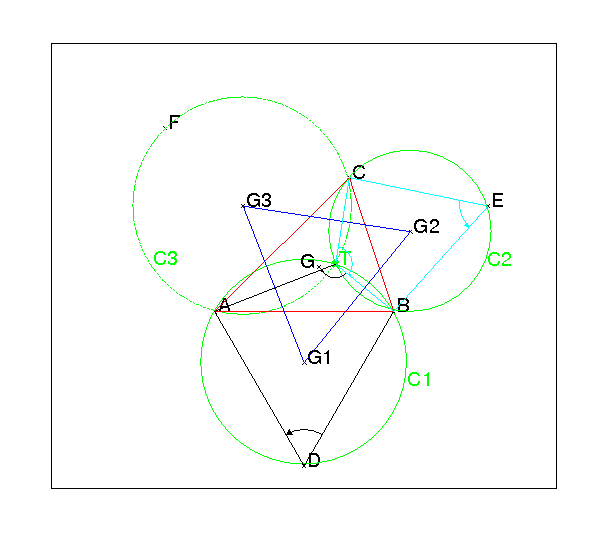
\includegraphics[width=8cm]{napo2}\\

Montrons que ces trois cercles sont concourants en un point $T$. \\
Soit $T$ le point d'intersection de $C_1$ et $C_2$, on a :\\
$\widehat{BDA}=\frac{\pi}{3}$.\\
Comme l'angle $\widehat{BTA}$ intercepte le m\^eme arc $BA$ que l'angle 
$\widehat{BDA}$ de $C_1$ on a :\\
$\widehat{BTA}=\frac{\pi}{3}$ ou $\widehat{BTA}=\frac{2\pi}{3}$ de m\^eme :\\ 
$\widehat{BTC}=\frac{\pi}{3}$ ou $\widehat{BTC}=\frac{2\pi}{3}$ donc :\\
soit $\widehat{CTA}=\widehat{BTC}+\widehat{BTA}$ si $TB$ est entre $TC$ et $TA$\\
soit $\widehat{CTA}=|\widehat{BTC}-\widehat{BTA}|$ sinon.\\
Donc  
$\widehat{CTA}=\frac{\pi}{3}$ ou $\widehat{CTA}=\frac{2\pi}{3}$ et donc
$CAFT$ sont cocycliques.\\
On a donc montr\'e que $T$ se trouve sur $C3$.\\
Comme $G_1G_2$ (resp $G_1G_3$  ou $G_2G_3$) est perpendiculaire \`a $BT$ (resp \`a $AT$ ou \`a $CT$) et que 
$\widehat{G_2G_1G_3}+\widehat{G_1G_2G_3}+\widehat{G_1G_3G_2}=\pi$ on a :\\
$\widehat{G_2G_1G_3}=\widehat{G_1G_2G_3}=\widehat{G_1G_3G_2}=\frac{\pi}{3}$\\
ce qui prouve que le triangle $G_1G_2G_3$ est \'equilat\`eral. 

\subsection{Avec $G_4$ le sym\'etrique de $G_1$ par rapport \`a $AB$}
Soit $G_4$ le sym\'etrique de $G_1$ par rapport \`a $AB$.\\

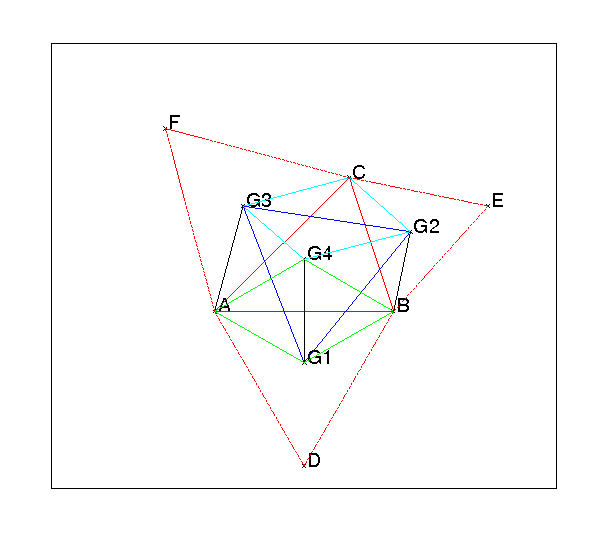
\includegraphics[width=8cm]{napo3}\\

Pour faire cette figure, on tape dans un \'editeur de programme : 
\begin{verbatim}
A:=point(-2.,-1.,'affichage'=0);
B:=point(2.,-1,'affichage'=0);
C:=point(1.,2,'affichage'=0);
D:=rotation(B,pi/3.,A);
E:=rotation(C,pi/3.,B);
F:=rotation(A,pi/3.,C);
G1:=isobarycentre(A,B,D);
G2:=isobarycentre(C,B,E);
G3:=isobarycentre(A,C,F);
G4:=symetrie(droite(A,B),G1);
G:=isobarycentre(A,C,B,affichage=quadrant2);
triangle(A,B,C,affichage=1);
triangle(G1,G2,G3,affichage=4);
segment(A,G1);
segment(A,G3);
segment(G4,G3);
segment(G4,G2);
segment(C,G2);
segment(C,G3);
segment(B,G4);
segment(A,G4);
segment(B,G2);
segment(B,G1);
segment(G4,G1);
segment(A,F,affichage=1+ligne_tiret);
segment(C,F,affichage=1+ligne_tiret);
segment(C,E,affichage=1+ligne_tiret);
segment(E,B,affichage=1+ligne_tiret);
segment(B,D,affichage=1+ligne_tiret);
segment(A,D,affichage=1+ligne_tiret);
\end{verbatim}

Les triangles $AG_4G_3$ et $G_4BG_2$ sont \'egaux et sont des triangles 
semblables \`a $ABC$ en effet :\\
le quadrilat\`ere $AG_1BG_4$ est un losange d'angle $A=\frac{\pi}{3}$ 
(4 cot\'es \'egaux \`a la diagonale $G_1G_4$), donc \\
l'angle $\widehat{G_4AG_3}$ est \'egale \`a l'angle $\widehat{BAC}$,\\
$AG_4=AG_1=BG_1=BG_4=\frac{AB}{\sqrt 3}$,\\
$AG_3=CG_3=\frac{AC}{\sqrt 3}$.\\
Le triangle $AG_4G_3$ est donc semblable au triangle $ABC$ avec comme rapport 
de similitude $\frac{1}{\sqrt(3)}$.\\
De m\^eme l'angle $\widehat{G_4BG_2}$ est \'egale \`a l'angle $\widehat{ABC}$ 
et,\\
$\displaystyle BG_2=CG_2=\frac{BC}{\sqrt 3}$\\
donc le triangle $G_4BG_2$ est semblable au triangle $ABC$ avec comme  rapport 
de similitude $\frac{1}{\sqrt 3}$.\\
On en d\'eduit que :\\
$BG_2=G_4G_3$ et $AG_2=G_4G_2$ et donc que le quadrilat\`ere $G_2CG_3G_4$ est 
un parall\'elogramme.\\
Les triangles $G_1G_4G_3$ et $G_1BG_2$ sont donc \'egaux (l'angle 
$\widehat{G_3G_4G_1}=\widehat{CBA}+pi/3=\widehat{G_2BG_1}$) et ces deux 
triangles se d\'eduisent l'un de l'autre par une rotaion de centre $G_1$ et 
d'anble $\frac{\pi}{3}$ donc \\
$G_1G_3=G_1G_2$  et l'angle $\widehat{G_2G_1G_3}=\frac{\pi}{3}$.\\
L'isobarycentre de $A,B,C$ est aussi l'isobarycentre de $G_1,G_4,C$ car le
quadrilat\`ere $AG_1BG_4$ est un losange.\\
L'isobarycentre de $G_1,G_4,C$ est aussi l'isobarycentre de $G_1,G_2,G_3$ car 
le quadrilat\`ere $CG_3G_4G_2$ est un parall\'elogramme.\\
Donc $ABC$ et $G_1G_2G_3$ ont m\^eme centre de gravit\`e.\\

\subsection{Avec les sym\'etriques de $G_1$ (resp de $G_2$) par rapport \`a $AB$ (resp \`a $BE$)}
\subsubsection{L'\'enonc\'e}
Soit $ABC$ un triangle quelconque. On construit \`a l'ext\'erieur du triangle 
 $ABC$ les triangles \'equilat\`eraux : $ABD$, $BCE$ et $ACF$.\\
1/ Montrer que $AE=BF=CD$.\\
2/ Montrer que $AE$, $BF$ et $CD$ sont concourantes.\\
3/ Th\'eor\`eme de Napol\'eon :\\
On note $G_1$, $G_2$ et $G_3$ les centres de gravit\'e des triangles 
$ABD$, $BCE$ et $ACF$.\\
Montrer que le triangle $G_1G_2G_3$ est \'equilat\`eral.\\

\subsubsection{La solution}
\begin{verbatim}
A:=point(-2.,-1.,'affichage'=0);
B:=point(2.,-1,'affichage'=0);
C:=point(0.,1.5,'affichage'=0);
D:=rotation(B,pi/3.,A);
E:=rotation(C,pi/3.,B);
F:=rotation(A,pi/3.,C);
segment(A,E,affichage=2);
segment(C,D,affichage=2);
segment(B,F,affichage=2+ligne_tiret);
T:=inter_droite(droite(A,E),droite(C,D),affichage=2+
                 epaisseur_point_2);
G1:=isobarycentre(A,B,D);
G2:=isobarycentre(C,B,E);
G3:=isobarycentre(A,C,F);
G:=isobarycentre(A,C,B,affichage=quadrant2);
triangle(A,B,C,affichage=1);
triangle(G1,G2,G3,affichage=4);
angle(B,D,A,"");
angle(B,C,E,"");
angle(C,E,B,"");
angle(C,A,F,"");
vecteur(B,G1,affichage=1)
vecteur(B,A,affichage=1);
vecteur(B,D,affichage=1);
vecteur(B,B+3*(G1-B),affichage=1);
vecteur(B,G2,affichage=6)
vecteur(B,E,affichage=6);
vecteur(B,C,affichage=6);
vecteur(B,B+3*(G2-B),affichage=6);
N:=rotation(C,pi/3.,T);
\end{verbatim}

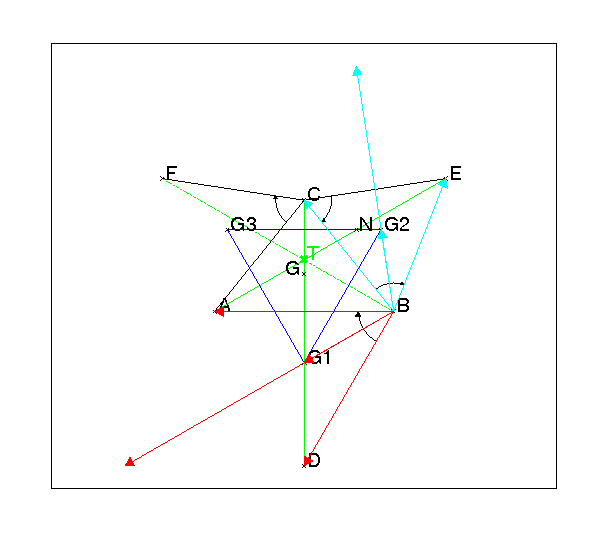
\includegraphics[width=8cm]{napo4}\\

On suppose le triangle $ABC$ direct.\\
1/ La rotation de centre $B$ et d'angle $-\pi/3$ transforme :\\
$D$ en $A$ et $C$ en $E$ donc:\\
 $DC=AE$ et 
$(\overrightarrow{DC},\overrightarrow{AE})=-\pi/3$.\\
De m\^eme la rotation de centre  $C$ et d'angle $-\pi/3$ transforme :\\
$E$ en $B$ et $A$ en $F$ donc :\\
 $AE=FB$ et 
$(\overrightarrow{EA},\overrightarrow{BF})=-\pi/3$.\\
On  montre, en utilisant les vecteurs, que $G_1G_2G_3$ est \'equilat\`eral, 
on a :\\
$\overrightarrow{BG_1}=\frac{1}{3}(\overrightarrow{BD}+\overrightarrow{BA})$
et
$\overrightarrow{BG_2}=\frac{1}{3}(\overrightarrow{BE}+\overrightarrow{BC})$\\
$\overrightarrow{CG_2}=\frac{1}{3}(\overrightarrow{CE}+\overrightarrow{CB})$
et
$\overrightarrow{CG_3}=\frac{1}{3}(\overrightarrow{CF}+\overrightarrow{CA})$\\
donc \\
$\overrightarrow{G_2G_1}=\frac{1}{3}(\overrightarrow{EA}+\overrightarrow{CD})$
 et \\
$\overrightarrow{G_2G_3}=\frac{1}{3}(\overrightarrow{BF}+\overrightarrow{EA})$\\
$\overrightarrow{BF}$ (resp $\overrightarrow{EA}$) est le transform\'e de 
$\overrightarrow{EA}$ (resp $\overrightarrow{CD}$) par une rotation d'angle 
$-\pi/3$ donc $\overrightarrow{G_2G_3}$ est le transform\'e de 
$\overrightarrow{G_2G_1}$ par une rotation d'angle $-\pi/3$ donc le triangle 
$G_1G_2G_3$ est \'equilat\`eral.\\
2/ Soit $T$ le point d'intersection de $AE$ et de $CD$. D'apr\`es la 
premi\`ere question :
$(\overrightarrow{TC},\overrightarrow{TE})=(\overrightarrow{DC},\overrightarrow{AE})=-\pi/3$.\\
On construit alors le point $N$ sur $AE$ pour que le triangle $TCN$ soit 
\'equlat\'eral et donc $(\overrightarrow{CN},\overrightarrow{CT})=-\pi/3$. 
Ainsi, la rotation de centre $C$ et d'angle $-\pi/3$ transforme $AE$ en $FB$
et le point $N$ de $AE$ en le point $T$ de $BF$ donc $BF$ passe par $T$.\\
3/ Autre d\'emonstration de $G_1G_2G_3$ est \'equilat\`eral.
On construit :\\
$G_4$ le sym\'etrique de $G_1$ par rapport \`a $AB$,\\ 
$G_5$ le sym\'etrique de $G_2$ par rapport \`a $BE$,\\
donc les triangles $AG_1G_4$, $BG_1G_4$, $BG_2G_5$ sont \'equilat\'eraux.\\
La rotation de centre $B$ et d'angle $-\pi/3$ transforme :\\
$G_1$ en $G_4$ et $G_2$ en $G_5$ donc $G_1G_2=G_4G_5$ et 
$(\overrightarrow{G_2G_1},\overrightarrow{G_5G_4})=-\pi/3$.\\
On va montrer que le quadrilat\`ere 
$G_3G_2G_5G_4$ est un parall\'elogramme et on aura ainsi montrer que le triangle $G_1G_2G_3$ est \'equilat\`eral puisque :\\
$G_3G_2=G_4G_5=G_1G_2$ et 
$(\overrightarrow{G_2G_3},\overrightarrow{G_5G_4})=0$ donc 
$(\overrightarrow{G_2G_3},\overrightarrow{G_2G_1})=\pi/3$.\\
Les triangles $AG_4G_3$ et $G_4BG_2$ sont semblables au triangle $ABC$ 
(m\^eme angle $A$ (resp $B$) et deux cot\'es proportionnels) et 
comme  $AG_4=G_4B$, les triangles $AG_4G_3$ et $G_4BG_2$ sont \'egaux.
Donc $G_3G_4=BG_2=BG_5=G_2G_5$.\\
On a :\\
$(\overrightarrow{G_4B},\overrightarrow{G_4G_3})=(\overrightarrow{G_4A},\overrightarrow{G_4G_3})+2\pi/3=(\overrightarrow{BG_4},\overrightarrow{BG_2})+2\pi/3=$\\
$(\overrightarrow{BG_4},\overrightarrow{BE})+2\pi/3-\pi/6=(\overrightarrow{BG_4},\overrightarrow{BE})+\pi/2$.\\
Donc $G_3G_4$ est parall\'ele \`a $G_2G_5$ puisque ces deux droites sont perpendiculaires \`a $BE$. On a ainsi montrer que le quadrilat\`ere 
$G_3G_2G_5G_4$ est un parall\'elogramme, ce qui termine la d\'emonstration. 
\subsection{Avec les nombres complexes}
Soient $a,b,c,g_1,g_2,g_2$ les affixes de $A,B,C,G_1,G_2,G_3$ on a :\\
si le triangle $ADB$ est de sens direct, $A$ se d\'eduit de $B$ dans la rotation de centre $g_1$ 
et d'angle $2*\pi/3$ donc puisque $j=e^{\frac{i2\pi}{3}}$:\\
$a-g_1=j*(b-g_1)$ \\
de m\^eme si les triangles $BEC$ et $CFA$ sont de sens direct on a :\\
$b-g_2=j*(c-g_2)$ \\
$c-g_3=j*(a-g_3)$ \\
On en d\'eduit que :\\
$(1-j)g_1=a-jb$ et\\
$(1-j)g_2=b-jc$ et\\
$(1-j)g_3=c-ja$ donc\\
$(1-j)(g_1-g_2)=a-b(1+j)+jc=a+jc+j^2b$ puisque $1+j+j^2=0$ et \\
$(1-j)(g_2-g_3)=b-c(1+j)+ja=j(a+jc+j^2b)$ puisque $j^3=1$ donc\\
$(1-j)(g_2-g_3)=j(1-j)(g_1-g_2)$ et apr\`es division par $j-1$ on a\\ 
$g_2-g_3=j(g_1-g_2)$ et\\
 cette \'egalit\'e prouve que le triangle $G_1G_2G_3$
est \'equilat\`eral.\\
On a de plus :\\
$(1-j)g_1+(1-j)g_2+(1-j)g_3=a-jb+b-jc+c-ja=(1-j)(a+b+c)$ donc\\
$(a+b+c)/3=(g_1+g_2+g_3)/3$ ce qui veut dire que les triangles $ABC$ et 
$G_1G_2G_3$ ont m\^eme centre de gravit\'e.
\section{La d\'emonstration du th\'eor\`eme avec {\tt Xcas}}
On suppose que le point {\tt A} est \`a l'origine du rep\`ere et que 
le point {\tt B} est le point d'affixe 2.
Le point {\tt C} a comme affixe $a+ib$, avec $a$ et $b$ quelconques.\\
Pour faire la figure on suppose que $a=-1$ et que $b=-1$.\\
On tape les instructions suivantes qui se trouvent dans le fichier 
{\tt napoleon} :
\begin{verbatim}
assume(a=0);
assume(b=1.5);
A:=point(-2,-1);
B:=point(2,-2);
C:=point(a,b);
T1:=couleur(triangle_equilateral(B,A),vert);
T2:=couleur(triangle_equilateral(C,B),vert);
T3:=couleur(triangle_equilateral(A,C),vert);
couleur(circonscrit(T1),vert);
couleur(circonscrit(T2),vert);
couleur(circonscrit(T3),vert);
AB:=segment(A,B);
AC:=segment(A,C);
CB:=segment(C,B);
G1:=normal(isobarycentre(T1));
G2:=normal(isobarycentre(T2));
G3:=normal(isobarycentre(T3));
G1G2:=couleur(segment(G1,G2),rouge);
G2G3:=couleur(segment(G2,G3),rouge);
G3G1:=couleur(segment(G3,G1),rouge);
normal(longueur2(G1,G2)-longueur2(G2,G3));
normal(longueur2(G1,G3)-longueur2(G3,G2));
\end{verbatim}

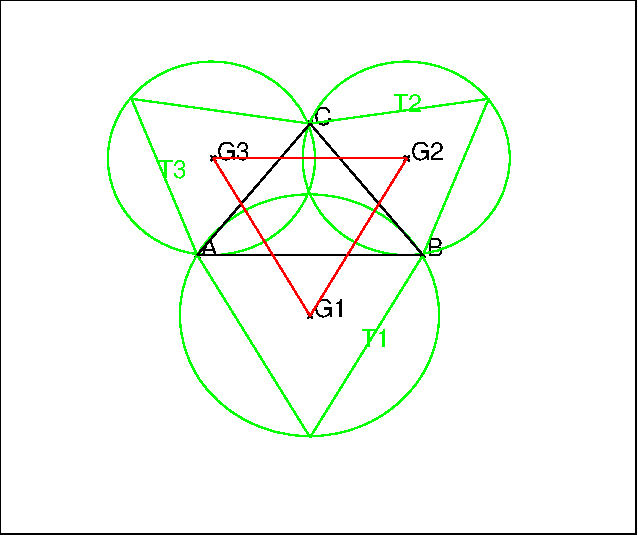
\includegraphics[width=\textwidth]{napo5}\\

On obtient la figure et comme r\'eponses  :\\
{\tt 0} \`a {\tt normal(longueur2(G1,G2)-longueur2(G2,G3));},\\
{\tt 0} \`a {\tt normal(longueur2(G1,G2)-longueur2(G1,G3));},\\
ce qui prouve que le triangle $G1G2G3$ est \'equilat\`eral.
\chapter{Des exercices sur les transformations}
\section{Exercice 1 sur les rotations}
\subsection{L'\'enonc\'e et sa figure}
Soit un triangle direct quelconque $ABC$. On construit \`a l'ext\'erieur de 
$ABC$ les carr\'es $ACDE$ et $AGHB$ et le parall\'elogramme $AEFG$.\\
Montrer que $BE=CG$ et que $CG$ est perpendiculaire \`a $EB$\\ 
Montrer que $AF=BC$ et que $AF$ est perpendiculaire \`a $BC$\\
Pour faire la figure, on d\'efinit le triangle direct $ABC$ avec les 3 points 
$A,B,C$ obtenus en cliquant en mode {\tt point}, puis on tape :
\begin{verbatim}
carre(A,C,D,E);
carre(B,A,G,H);
F:=translation(G-A,E);
parallelogramme(A,E,F);
segment(B,E,affichage=1);
segment(C,G,affichage=1);
segment(B,C,affichage=2);
segment(A,F,affichage=2);
K:=projection(droite(B,C),A):;
segment(A,K,affichage=4+ligne_tiret_point);
\end{verbatim}
On obtient :
\begin{center}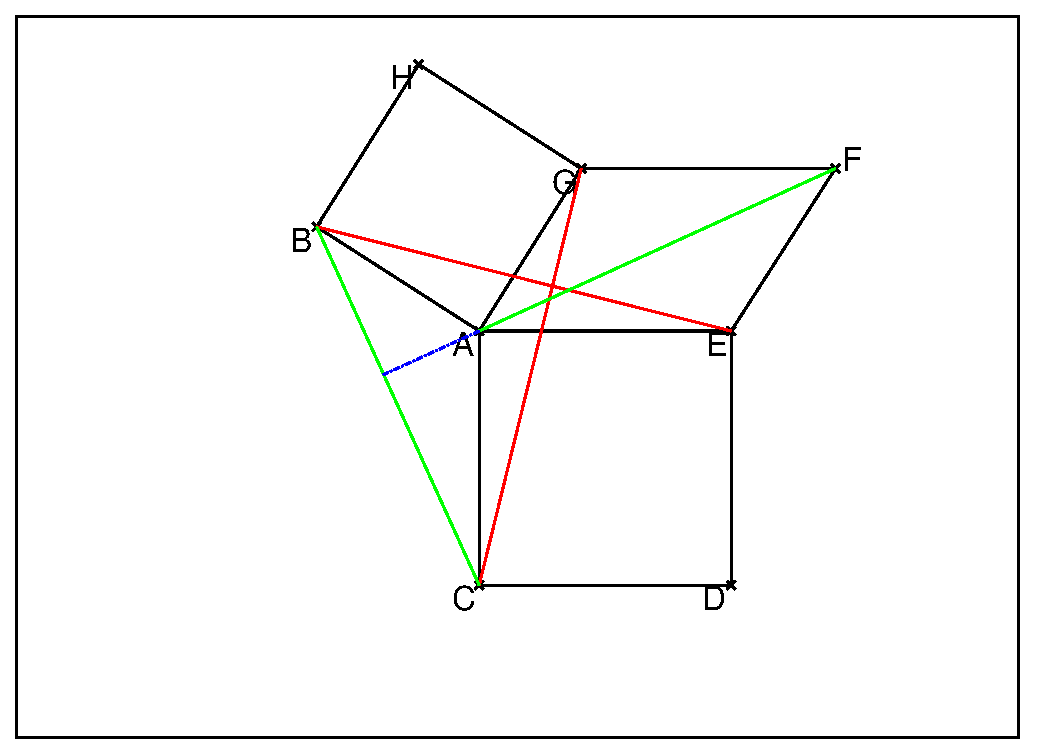
\includegraphics[width=\textwidth]{rota}\end{center}
\subsection{La d\'emonstration g\'eom\'etrique}
La rotation de centre $A$ et d'angle $\frac{\pi}{2}$ transforme $C$ en $E$ et 
$G$ en $B$. Donc $CG=EB$ et $CG$ est perpendiculaire \`a $EB$\\
Soit $I$ le sym\'etrique de $G$ par rapport \`a $A$ :
\begin{center}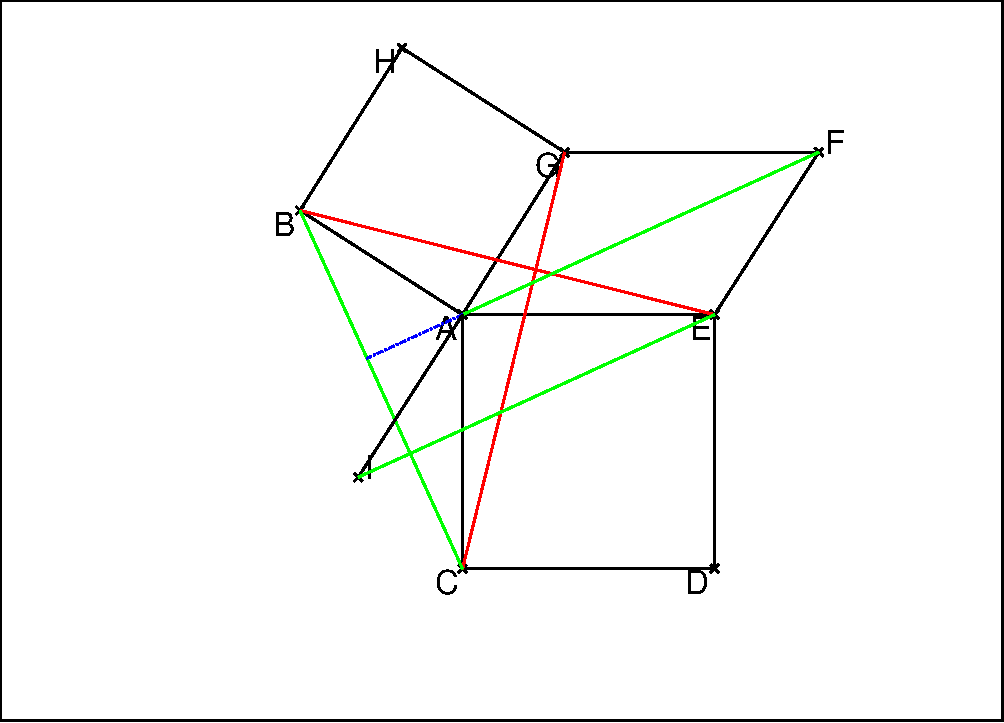
\includegraphics[width=\textwidth]{rotat}\end{center}
On a donc :\\
$\overrightarrow{IA}=\overrightarrow{AG}=\overrightarrow{EF}$  donc le 
quadrilat\`ere $AIEF$ est un parall\'elogramme donc :\\
$\overrightarrow{AF}=\overrightarrow{IE}$
La rotation de centre $A$ et d'angle $\frac{\pi}{2}$ transforme $B$ en $I$ donc
$BC=IE$ et $BC$ est perpendiculaire \`a $IE$ et comme
$\overrightarrow{AF}=\overrightarrow{IE}$, on en d\'eduit que :
$BC=AF$ et $BC$ est perpendiculaire \`a $AF$.
\subsection{La d\'emonstration avec les nombres complexes}
On choisit un rep\`ere d'origine $A$.\\
La rotation de centre $A$ et d'angle $\frac{\pi}{2}$ transforme $C$ en $E$ et 
$G$ en $B$. Donc si $zb,zc,...$ d\'esigne les affixes de $B,C...$ on a :\\
$ze=i*zc$ et $zb=i*zg$ donc $zg=-i*zb$\\
$\overrightarrow{AF}=\overrightarrow{AE}+\overrightarrow{AG}$ donc \\
$zf=ze+zg=i(zc-zb)$ donc
$AF=BC$ et $BC$ est perpendiculaire \`a $AF$.
\subsection{La d\'emonstration avec {\tt Xcas}}
On choisit un rep\`ere d'origine $A$ et $C$ sur l'axe des $y$.\\
On tape :
\begin{verbatim}
assume(a=[-2,-5,5,0.1]);
assume(b=[1,-5,5,0.1]);
assume(c=[-5/2,-5,5,0.1]);
A:=point([0,0,'affichage'=0]);
B:=point([a,b,'affichage'=0]);
C:=point([0,c,'affichage'=0]);
carre(A,C,D,E);
carre(B,A,G,H);
F:=translation(G-A,E);
parallelogramme(A,E,F);
\end{verbatim}
Puis on demande \`a {\tt Xcas} :\\
{\tt longueur2(C,G)}, on obtient {\tt (-b)\verb|^|2+(c+a)\verb|^|2}\\
{\tt longueur2(B,E)}, on obtient {\tt (a+c)\verb|^|2+(b-c+c)\verb|^|2 }\\
{\tt longueur2(A,F)}, on obtient {\tt (c-b)\verb|^|2+a\verb|^|2 }\\
{\tt longueur2(B,C)}, on obtient {\tt a\verb|^|2+(b-c)\verb|^|2 }\\
{\tt equation(droite(C,G))}, on obtient {\tt y=((-a-c)*1/b*x+c) }\\
{\tt equation(droite(B,E))}, on obtient {\tt y=(b*1/(a+c)*x+(b*c)/(a+c)) }\\
le produit des pentes vaut bien -1.\\
{\tt equation(droite(A,F))}, on obtient {\tt y=((-a)*1/(b-c)*x)}\\
{\tt equation(droite(B,C))}, on obtient {\tt y=((b-c)*1/a*x+c)}\\
le produit des pentes vaut bien -1.\\
On peut aussi utiliser directement :\\
{\tt normal(pente(droite(C,G))*pente(droite(B,E)))} et\\
{\tt normal(pente(droite(A,F))*pente(droite(B,C)))} et obtenir {\tt -1}\\
ou \\
{\tt est\_perpendiculaire(droite(C,G),droite(B,E))} et\\
{\tt est\_perpendiculaire(droite(A,F),droite(B,C))} et obtenir {\tt 1}
\section{Exercice 2 sur les similitudes}
\subsection{L'\'enonc\'e et sa figure}
Soit un carr\'e direct $ABCD$ de centre $I$ et de c\^ot\'e $a$. Soit $J$ le 
milieu de $IB$.
On construit le carr\'e direct $IJKL$.\\
Trouver le centre, le rapport et l'angle de la similitude qui transforme :\\
$A$ en $I$,\\
$B$ en $J$\\
$C$ en $K$ et\\
$D$ en $L$.\\
On tape :
\begin{verbatim}
A:=point(0);
assume(a=[5,0,10,0.1]);
B:=point(a);
c:=carre(A,B,C,D):;c
I:=milieu(A,C);
J:=milieu(B,I);
carre(I,J,K,L);
segment(A,C);
segment(B,D);
\end{verbatim}
On obtient :
\begin{center}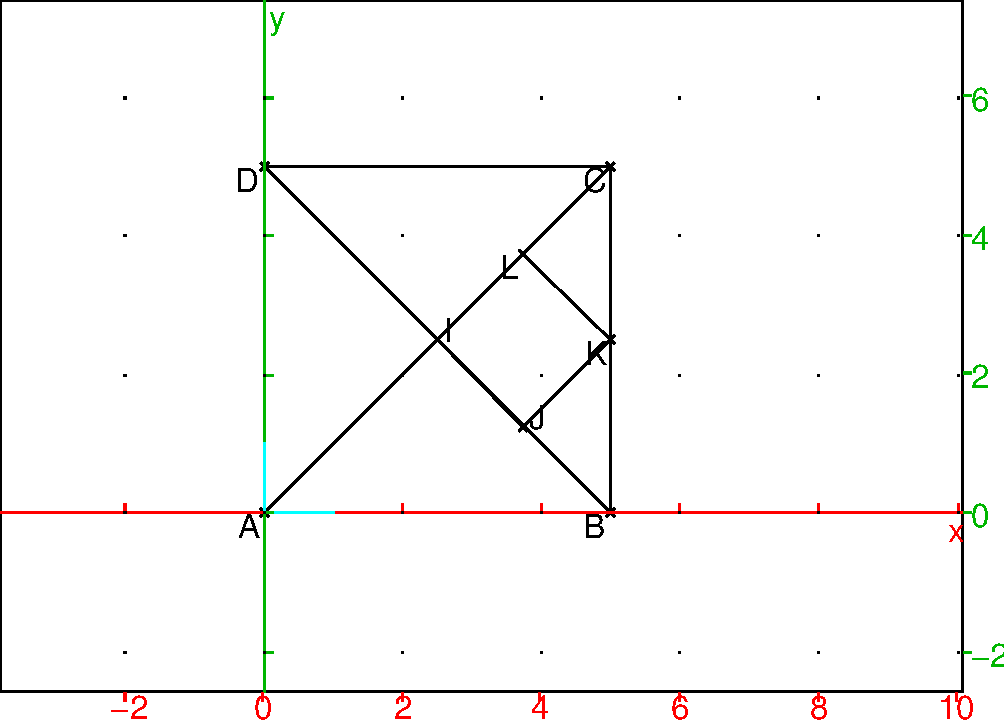
\includegraphics[width=\textwidth]{simili}\end{center}

\subsection{La d\'emonstration g\'eom\'etrique} 
Si cette similitude existe on a :\\
le rapport de la similitude est 
$k=a*\sqrt{2}/4$.puisque $IJ=a*\sqrt{2}/4=AB*\sqrt{2}/4$, \\
L'angle est de $-\frac{\pi}{4}$ puisque 
$(\overrightarrow{AB},\overrightarrow{IJ})=-\frac{\pi}{4}$\\
Cherchons son centre $O$.\\
On doit avoir $(\overrightarrow{OA},\overrightarrow{OI})=-\frac{\pi}{4}$
donc $O$ se trouve sur l'arc $ABI$ du cercle de diam\`etre $AB$ (arc capable 
interceptant $AI$ et d'angle $-\frac{\pi}{4}$ puisque
l'angle au centre de ce cercle qui intercepte l'arc $AI$ est droit).\\
On doit avoir $(\overrightarrow{OB},\overrightarrow{OJ})=-\frac{\pi}{4}$
donc $O$ se trouve sur l'arc $BKJ$ du cercle de diam\`etre $BK$ (arc capable
interceptant $BJ$ et d'angle $-\frac{\pi}{4}$ puisque l'angle au centre de ce 
cercle qui intercepte l'arc $BJ$ est droit).\\
Soit $O$ l'intersection de ces 2 arcs : $O$ est donc la projection de $B$ sur
$AK$ (puisque l'angle $(\overrightarrow{OA},\overrightarrow{OB})=\frac{\pi}{2}$
et l'angle $(\overrightarrow{OB},\overrightarrow{OK})=\frac{\pi}{2}$, on a
$(\overrightarrow{OA},\overrightarrow{OK})=\pi$).\\
La similitude de centre $O$, d'angle
$-\frac{\pi}{4}$ et de rapport $k=a*\sqrt{2}/4$ transforme $A$ en $I$ et $B$ en
$J$. Comme une similitude transforme des longueurs \'egales en des longueurs 
\'egales et conserve aussi les angles, cette similitude transforme le carr\'e
direct $ABCD$ en le carr\'e direct $IJKL$.\\
On peut donc en d\'eduire que les 4 cercles :\\
{\tt cercle(A,B),cercle(B,K),circonscrit(I,K,C),circonscrit(ADL)} \\
sont concourants en $O$. \\
En effet :\\
$(\overrightarrow{IC},\overrightarrow{IK})=-\frac{\pi}{4}$ donc $I$ et $O$ sont sur l'arc capable interceptant $CK$ et d'angle $-\frac{\pi}{4}$. On en d\'eduit que $O$ est sur le cercle circonscrit \`a $IKC$.\\
De m\^eme $(\overrightarrow{AD},\overrightarrow{AL})=-\frac{\pi}{4}$ donc $A$ 
et $O$ sont sur l'arc capable interceptant $CK$ et d'angle $-\frac{\pi}{4}$. 
On en d\'eduit que $O$ est sur le cercle circonscrit \`a $JAD$.
\begin{center}\includegraphics[width=\textwidth]{similit}\end{center}
\subsection{La d\'emonstration avec les nombres complexes et {\tt Xcas}}
On choisit $A$ \`a l'origine et $B$ sur l'axe des $x$.\\
Si cette similitude existe on a :\\
le rapport de la similitude est 
$k=a*\sqrt{2}/4$.puisque $IJ=a*\sqrt{2}/4=AB*\sqrt{2}/4$, \\
L'angle est de $-\frac{\pi}{4}$ puisque 
$(\overrightarrow{AB},\overrightarrow{IJ})=-\frac{\pi}{4}$\\
Cherchons $O$ le centre de la similitude d'affixe $z0$, on a :\\
$-z0*\sqrt 2/4*exp(-i*\pi/4)=a*(1+i)/2-z0$
On tape :\\
{\tt normal(solve(-z0*sqrt( 2)/4*exp(-i*pi/4)=a*(1+i)/2-z0,z0))}\\
On obtient :\\
{\tt [(4+2*i)/5*a]}\\
donc $z0=(4+2*i)/5*a$
On tape :\\
{\tt I:=similitude(point((4+2*i)/5*a),sqrt(2)/4,-pi/4,A,\\
affichage=1+epaisseur\_point\_2)}\\
{\tt J:=similitude(point(4+2*i),sqrt( 2)/4,-pi/4,B,\\
affichage=1+epaisseur\_point\_2)}\\
{\tt K:=similitude(point(4+2*i),sqrt( 2)/4,-pi/4,C,\\
affichage=1+epaisseur\_point\_2)}\\
{\tt L:=similitude(point(4+2*i),sqrt( 2)/4,-pi/4,D,\\
affichage=1+epaisseur\_point\_2)}\\
On obtient :\\
\begin{center}\includegraphics[width=\textwidth]{similitu}\end{center}
\section{Exercice 3 : lieu et similitude}
\subsection{L'\'enonc\'e et sa figure}
Soit un triangle direct $OAB$ rectangle en $O$ avec $OA=a$ et $OB=b$.\\
Soit $D=At$ une demi droite variable telle que :\\
$(\overrightarrow{OA},\overrightarrow{At})=c$, $0 \leq c \leq \frac{\pi}{2}$.\\
Soient $A1$ et $B1$ les projections respectives de $A$ et $B$ sur $D$.\\
Quelle est la valeur de $c$ pour laquelle $A1$ et $B1$ sont confondus en un 
point que l'on nommera $P$ ?
Trouver les lieux de $A1$ et de $B1$ quand $c$ varie.\\
Montrer que le triangle $PA1B1$ reste semblable au triangle $OAB$ quand $c$ 
varie.\\
Trouver le lieu de $M$ milieu de $A1B1$ quand $c$ varie.\\
On tape (on choisit $a=3$ et $b=5$):
(les instructions {\tt carre} sont la pour voir les droites perpendiculaires)
\begin{verbatim}
assume(a=3);
assume(b=5);
O:=point(0);
A:=point(a);
B:=point(b*i);
d:=segment(A,B);
supposons(c=[0.8,0,1.57,0.1]);
D:=droite(y=(tan(c)*x));
A1:=projection(D,A);
B1:=projection(D,B);
P:=projection(d,O);
carre(P,O+(P-0)*0.9);
segment(O,P,affichage=3+point_tiret);
carre(P,O+(P-0)*0.9);
carre(O+(P-0)*0.93,P);
segment(A,A1,affichage=3+point_tiret);
carre(A1,O+(A1-0)*0.9);
segment(B,B1,affichage=3+point_tiret);
carre(B1,O+(B1-0)*1.05);
triangle(P,A1,B1);
M:=milieu(A1,B1);
C1:=cercle(1.5,1.5,0,pi);
C2:=cercle(2.5*i,2.5,-pi/2,pi/2);
C3:=similitude(P,sqrt(a^2+b^2)/(2*b),atan(a/b),C2,affichage=5)
\end{verbatim}
On obtient :
\begin{center}\includegraphics[width=\textwidth]{simi}\end{center}
\subsection{La d\'emonstration g\'eom\'etrique} 
$A1$ et $B1$ sont confondus lorsque $D$ est perpendiculaire \`a $AB$.
$P$ est donc la projection de $O$ sur $AB$.\\
Quand $c$ varie, l'angle $(\overrightarrow{A1O},\overrightarrow{A1A})=\frac{\pi}{2}$ donc le lieu de $A1$ est le demi-cercle $C1$ de diam\`etre $OA$ contenant $P$.\\
Quand $c$ varie l'angle $(\overrightarrow{B1B},\overrightarrow{B1O})=\frac{\pi}{2}$ donc le lieu de $B1$ est le demi-cercle $C2$ de diam\`etre $OB$ contenant $P$.\\
Ces deux demi-cercles se coupent en $P$.\\
Les triangles $POA$ et $PBO$ sont semblables au triangle $OBA$.\\
Si $B1$ est sur l'arc $OP$ de $C2$ alors $A$ est sur l'arc $AP$ de $C1$.\\ 
alors l'angle 
Si $B1$ est sur l'arc $PB$ de $C2$ alors $A$ est sur l'arc $OP$ de $C1$.\\ 
Dans les 2 cas l'angle $B1$ de $PA1B1$ est \'egal \`a l'angle $B$ de $OAB$ et 
$A1$ de $PA1B1$ est \'egal \`a l'angle $A$ de $OAB$.\\
Donc le triangle $PB1A1$ est direct et est semblable au triangle $OBA$.\\
On en d\'eduit que $A1$ se d\'eduit de $B1$ par une similitude de centre $P$,
d'angle $\pi/2$ et de rapport $PA1/PB1=OA/OB=a/b$. $C1$ est donc l'image de 
$C2$ par cette similitude.\\
Le milieu $M$ de $A1B1$ se d\'eduit de $B1$ par une similitude de centre $P$,
d'angle :\\
$B1$ (\'egal \`a l'angle $B$ de $OAB$ valant atan$(a/b)$) et de rapport :\\
$PM/PB1=AB/(2*OB)=\sqrt{a^2+b^2}/(2b)$ (car la m\'ediane $OK$ de $OAB$ a pour 
longueur $AB/2=\sqrt{a^2+b^2}/2$).\\
Donc le lieu de $M$ est le demi cercle $C3$ qui se d\'eduit de $C2$ par cette 
similitude : c'est le demi-cercle diam\`etre le segment joingnant les milieux de $OA$ et $OB$ (car si $c=0$ $A1$ est en $A$ et $B1$ est en $O$ et si
$c=\pi/2$ $A1$ est en $O$ et $B1$ est en $B$) 
qui passe par $P$ (puisque quand $A1$ et $B1$ sont en $P$, $M$milieu de $A1B1$ 
est aussi en $P$). 
\begin{center}\includegraphics[width=\textwidth]{simil}\end{center}

\subsection{La d\'emonstration avec les nombres complexes et {\tt Xcas}}
$P$ est la projection de $O$ sur $AB$.\\
On $PO*AB=a*b=PO*\sqrt{a^2+b^2}$ donc $O-P=(B-A)*(iab/(a^2+b^2))$
si $p$ est l'affixe de $P$ on a : \\
$p=(a-ib)(iab/(a^2+b^2))=(ab^2+ia^2b)/(a^2+b^2)$\\
$A1$ a pour affixe $a1=a\cos(c)\exp(ic)$\\
$B1$ a pour affixe $b1=b\sin(c)\exp(ic)$\\
$M$ a pour affixe $m=(a1+b1)/2=(a\cos(c)+b\sin(c))\exp(ic)/2$\\
On pose :\\
$x1=$re$(m)=(a\cos(c)+b\sin(c))\cos(c)/2$ et \\
$y1=$im$(m)=(a\cos(c)+b\sin(c))\sin(c)/2$\\
On a $x1\geq 0$ et $y1\geq 0$ car $c\in [0;\pi/2]$.\\
On tape :\\
{\tt x1,y1:=op(normal(coordonnees(M)))}\\
{\tt factor(equation(plotparam(x1+i*y1,c)))}\\
On obtient :\\
{\tt (b\verb|^|2+a\verb|^|2)*(2*x\verb|^|2-x*a-b*y+2*y\verb|^|2)}\\
qui est l'\'equation du cercle de centre d'affixe $(a+ib)/2$ passant par $O$.\\
Comme $A1$ et $B1$ se trouve dans l'angle 
$(\overrightarrow{OA},\overrightarrow{OB})$ c'est le demi-cercle se trouvant dans cet angle qui est le lieu de $M$.\\
ou bien, on calcule :\\
$x1^2+y1^2=(a\cos(c)+b\sin(c))^2/4=$\\
$a/4*\cos(c)(a\cos(c)++b\sin(c))+b/4\sin(c)(a\cos(c)++b\sin(c))=$\\
$a*x1/2+b*y1/2$\\
Donc le lieu de $M$ a pour \'equation pour $x\geq 0$ et $y\geq 0$ :\\
$x^2+y^2-ax/2-by/2=(x-a/4)^2+(y-b/4)^2-(a^2+b^2)/16$ \\ 
qui est l'\'equation du demi-cercle $C3$.
\chapter{Le th\'eor\`eme de Morley}
\section{Le th\'eor\`eme}
Soit un triangle $ABC$ et ses trissectrices int\'erieures.\\
Soient $P,Q,R$ les points de ces trissectrices tels que le triangle $ABP$ 
(respectivement $BCQ$, $CAR$) ait comme angles
  $\frac{\widehat A}{3}$ et $\frac{\widehat B}{3}$ (respectivement 
$\frac{\widehat B}{3}$ et $\frac{\widehat C}{3}$, $\frac{\widehat C}{3}$ et 
$\frac{\widehat A}{3}$), alors le triangle $PQR$ est \'equilat\'eral.\\
De plus si $U,\ V,\ W $ sont les points de ces trissectrices tels que le 
triangle $ABU$ (respectivement $BCV$, $CAW$) ait comme angles 
$\frac{\widehat 2A}{3}$ et 
$\frac{\widehat 2B}{3}$ (respectivement $\frac{\widehat 2B}{3}$ et 
$\frac{\widehat 2C}{3}$, $\frac{\widehat 2C}{3}$
et $\frac{\widehat 2A}{3}$), 
alors les triangles $URQ$, $VRP$, $WPQ$ sont isoc\`eles.\\
On remarquera que le triangle isoc\`ele $URQ$ a comme angles :\\
$\widehat{U}=\pi-\frac{\widehat 2A}{3}-\frac{\widehat 2B}{3}$\\
$\widehat{R}=\widehat{Q}=\frac{\widehat A}{3}+\frac{\widehat B}{3}$. 

\section{La figure}
On prend comme param\`etres {\tt a1} et {\tt b1} qui repr\'esentent le tiers 
des angles {\tt A} et {\tt B} du triangle {\tt ABC}.\\
Quitte \`a faire une similitude, on peut choisir {\tt A} \`a l'origine du 
rep\`ere et {\tt B} au point d'affixe 1, le point {\tt C} a alors 
comme affixe :
$$\frac{\tan(3*b1)}{\tan(3*a1)+\tan(3*b1)*(1+i*\tan(3*a1))}$$
$C$ est donc sur la droite passant par $A$ de pente $\tan(3*a1)$ et sur la 
droite passant par $B$ et de pente $-tan(3*b1)$.\\
On tape :
\begin{verbatim}
A:= point(-4.95-1.777*i); 
B:= point(3.786-2.876*i);
C:= point(0.722+1.9*i);
a1:=(angle(A,B,C))/3;  
b1:=(angle(B,C,A))/3;  
c1:=eval(pi/3-a1-b1);  
P:=inter(rotation(A,a1,droite(A,B)),rotation(B,-b1,   
                                    droite(B,A)))[0];  
Q:=inter(rotation(C,-c1,droite(C,B)),rotation(B,b1,
                                    droite(B,C)))[0];  
R:=inter(rotation(A,-a1,droite(A,C)),rotation(C,c1,
                                    droite(C,A)))[0]; 
U:=inter(rotation(A,2*a1,droite(A,B)),rotation(B,-2*b1,
                                    droite(B,A)))[0];  
V:=inter(rotation(C,-2*c1,droite(C,B)),rotation(B,2*b1,
                                    droite(B,C)))[0];  
W:=inter(rotation(A,-2*a1,droite(A,C)),rotation(C,2*c1,
                                    droite(C,A)))[0]; 
triangle(A,R,C);
triangle(B,Q,C);
triangle(A,P,B);
triangle(P,Q,R);
triangle(U,Q,R);
triangle(V,P,R);
triangle(W,Q,P); 
\end{verbatim}
{\bf Remarque}
On peut aussi utiliser la d\'efinition d'une droite par un point et sa pente 
pour d\'efinir les points {\tt C} et {\tt P} ce qui nous dispense faire les 
calculls des coordonn\'ees de {\tt C} et {\tt P}.\\
On peut aussi taper :
\begin{verbatim}
A:=point(0);
B:=point(1);
a1:=0.32;
b1:=0.42;
TA1:=droite(A,pente=tan(a1));
TA2:=droite(A,pente=tan(2a1));
TA3:=droite(A,pente=tan(3a1)):;
TB1:=droite(B,pente=-tan(2b1)):;
TB2:=droite(B,pente=-tan(b1)):;
TB3:=droite(B,pente=-tan(3b1)):;
C:=inter_unique(TA3,TB3);
TC1:=droite(C,pente=tan(2a1-b1+pi/3)):;
TC2:=droite(C,pente=tan(a1-2b1+2pi/3)):;
TC3:=droite(C,pente=tan(3a1+pi/3)):;
P:=inter_unique(TA1,TB2);
Q:=inter_unique(TB1,TC2);
R:=inter_unique(TC1,TA2);
triangle(A,R,C);
triangle(B,Q,C);
triangle(A,P,B);
triangle(P,Q,R,couleur=magenta+line_width_2);
pq2:=longueur2(P,Q);
pr2:=longueur2(P,R);
qr2:=longueur2(Q,R);
U:=inter_unique(TB1,TA2);
V:=inter_unique(TB2,TC1);
W:=inter_unique(TC2,TA1)
normal(longueur2(W,Q)-longueur2(W,P));
normal(longueur2(U,Q)-longueur2(U,R));
normal(longueur2(V,P)-longueur2(V,R));
angle(A,B,W,"a1");
angle(B,V,A,"b1");
polygone(W,Q,U,R,V,P,affichage=vert);
\end{verbatim}
On obtient la figure du triangle de Morley :\\

\includegraphics[width=\textwidth]{morley1}\\

et {\tt 0.0379352631434} comme valeur des carr\'es des 3 longueurs et des 
valeurs de l'ordre de $10^{-14}$ pour les diff\'erence de longueurs.\\
Mais cela n'est pas une d\'emonstration....


\section{La d\'emonstration du th\'eor\`eme avec {\tt Xcas}}
On place {\tt A} \`a l'origine, {\tt B} en (1,0) et on utilise 2 param\`etres 
{\tt a1} et {\tt b1}, tels que les angles en {\tt A} et {\tt B} soient 
{\tt 3*a1}, {\tt 3*b1}
{\tt C} est donc sur la droite passant par {\tt A} de pente {\tt tan(3*a1)} et 
sur la droite passant par {\tt B} et de pente {\tt -tan(3*b1)}, etc.\\
Pour faire une d\'emonstration avec {\tt Xcas}, on va remplacer :
{\tt a1:=0.32;} par {\tt assume(a1=0.32);} et\\
{\tt b1:=0.42;} par {\tt assume(b1=0.42);}\\
La figure reste la m\^eme mais les calculs sont faits avec les param\`etres 
formels {\tt a1} et {\tt b1}:
\begin{verbatim}
assume(a1=0.32);
assume(b1=0.42);
A:=point(0);
B:=point(1);
TA1:=droite(A,pente=tan(a1));
TB1:=droite(A,pente=texpand(tan(2a1)));
TA3:=droite(A,pente=texpand(tan(3a1))):;
TB1:=droite(B,pente=-texpand(tan(2b1))):;
TB2:=droite(B,pente=-tan(b1)):;
TB3:=droite(B,pente=-texpand(tan(3b1))):;
C:=inter_unique(TA3,TB3);
TC1:=droite(C,pente=texpand(tan(2a1-b1+pi/3))):;
TC2:=droite(C,pente=texpand(tan(a1-2b1+2pi/3))):;
TC3:=droite(C,pente=texpand(tan(3a1+pi/3))):;
P:=inter_unique(TA1,TB2);
Q:=inter_unique(TB1,TC2);
R:=inter_unique(TC1,TA2);
triangle(A,R,C);
triangle(B,Q,C);
triangle(A,P,B);
triangle(P,Q,R,couleur=magenta+line_width_2);
pq2:=longueur2(P,Q);
pr2:=longueur2(P,R);
qr2:=longueur2(Q,R);
U:=inter_unique(TB1,TA2);
V:=inter_unique(TB2,TC1);
W:=inter_unique(TC2,TA1)
angle(A,B,W,"a1");
angle(B,V,A,"b1");
polygone(W,Q,U,R,V,P,affichage=vert);
normal(pq2-pr2),normal(pq2-qr2);
normal(longueur2(W,Q)-longueur2(W,P));
normal(longueur2(U,Q)-longueur2(U,R));
normal(longueur2(V,P)-longueur2(V,R));
\end{verbatim}

Ou on tape dans un \'editeur de programme 
\begin{verbatim}
assume(a1=0.32); 
assume(b1=0.42);
A:=point(0);
B:=point(1);
C:=point(texpand(tan(b1*3)/(tan(a1*3)+
                 tan(b1*3))*(1+i*tan(a1*3))));
P:=point(texpand(tan(b1)/(tan(a1)+
                 tan(b1))*(1+i*tan(a1))));
R:=(inter(droite(0,1+i*texpand(tan(2*a1))),
      droite(C,C+1+i*texpand(tan(pi/3+2*a1-b1)))))[0];
Q:=(inter(droite(1,i*texpand(tan(2*b1))),
      droite(C,C+1+i*texpand(tan(2*pi/3+a1-2*b1)))))[0];
U:=point(texpand(tan(2*b1)/(tan(2*a1)+
                 tan(2*b1))*(1+i*tan(2*a1))));
W:=(inter(droite(0,1+i*texpand(tan(a1))),
      droite(C,C+1+i*texpand(tan(2*pi/3+a1-2*b1)))))[0];
V:=(inter(droite(1,i*texpand(tan(b1))),
       droite(C,C+1+i*texpand(tan(pi/3+2*a1-b1)))))[0];
triangle(A,R,C);
triangle(B,Q,C);
triangle(A,P,B);
triangle(P,Q,R);
triangle(P,Q,W);
triangle(P,V,R);
triangle(U,Q,R);
pq2:=longueur2(P,Q);
pr2:=longueur2(P,R);
qr2:=longueur2(Q,R);
ur2:=longueur2(U,R);
uq2:=longueur2(U,Q);
vr2:=longueur2(V,R);
vp2:=longueur2(V,P);
pw2:=longueur2(P,W);
qw2:=longueur2(Q,W);
normal(pq2-pr2),normal(pq2-qr2);
normal(uq2-ur2);
normal(vp2-vr2);
normal(pw2-qw2);
\end{verbatim}
On valide par {\tt OK}

On obtient alors  :\\
{\tt 0,0,0,0,0}\\
ce qui prouve que le triangle {\tt PQR} est \'equilat\'eral et que les 
triangles {\tt UQR}, {\tt VPR} et {\tt WPQ} sont isoc\`eles.

%On obtient :

%\begin{center}\includegraphics[width=15cm]{morleyp}\end{center}

\subsection{Une d\'emonstration g\'eom\'etrique}
{\tt La figure}\\

\begin{center}\includegraphics[width=10cm]{morley2}\end{center}
{\tt La d\'emonstration}\\
On suppose que les angles du triangle $ABC$ valent $3a,3b,3c$ 
($a+b+c=\pi/3$).\\
On trace les trissectrices des angles $B$ et $C$.\\ 
Soit $D$ l'intersection des deux trissectrices tels que le triangle $BCD$ aient
 comme angles $b$ et $c$ et $\pi-b-c$.\\
Soient $F$ et $H$ tels que le triangle $HFD$ soit isoc\'ele d'angle \`a la base
 $a+c$ et $H$ sur $CD$ et $F$ sur la 2-i\`eme trissectrice de $B$ : on 
construit $F$ sur la 2-i\`eme trissectrice de $B$ tel que l'angle 
$\widehat{FDB} =\pi/3+c=a+c+b+c$,\\
Soient $E$ et $K$ tels que le triangle $KED$ soit isoc\'ele d'angle \`a la base
 $a+b$ et $K$ sur $BD$ et $E$ sur la 2-i\`eme trissectrice de $C$ : on 
construit $F$ sur la 2-i\`eme trissectrice de $C$ tel que l'angle 
$\widehat{CDK} =\pi/3+b=a+b+b+c$)\\
On a :\\
$\widehat{HDB}=b+c=\widehat{KDC}$\\
$\widehat{FDE}+(a+c)+(b+c)+(\pi-b-c)+(a+b)+(b+c)=2\pi$ donc,\\
$\widehat{FDE}=\pi-2a-2b-2c=\pi/3$ et \\
$\widehat{BFD}=\pi-b-(a+c)-(b+c)=a+\pi/3$\\
$\widehat{CED}=\pi-c-(a+b)-(b+c)=a+\pi/3$\\
$D$ est sur les bissectrices des angles $\widehat{CBF}$ et $\widehat{BCE}$, 
donc $D$ est \'equidistant de $BF$ et $CE$ et puisque $\widehat{BFD}=\widehat{CED}$ on a $DE=DF$\\
donc le triangle $DEF$ est \'equilat\`eral ($DE=DF$ et $\widehat{FDE}=\pi/3$).\\
Il reste donc \`a montrer que $F$ et $E$ sont sur les trissectrices de $A$ :
on va montrer que $FH$ et $EK$ sont les trissectrices de $A$.\\
$FK$ est la bissectrice de $\widehat{DKE}$ \\
$FB$ est la bissectrice de $\widehat{DBA}$ donc \\
si on suppose que $KE$ coupe $AB$ an $L$, $LF$ est la bissectrice de 
$\widehat{L}$ et
$\widehat{BLF}=\widehat{FLK}=a$ ($\widehat{BKL}=\pi-2(a+b)$ $\widehat{KBL}=2b$ 
donc $\widehat{BLK}=2a$) et comme $\widehat{BFH}=a+b$,
$L,F,H$ sont align\'es.\\
De m\^eme si on suppose que $HF$ coupe $AC$ en $J$, $JE$ est la bissectrice 
de $\widehat{J}$ et
$\widehat{CJE}=\widehat{EJH}=a$ et $J,E,K$ sont align\'es.\\
On a $K,E,L$ sont align\'es et $J,E,K$ sont align\'es.\\
On a $L,F,H$ sont align\'es et $F,H,J$ sont align\'es\\
donc $J$ et $L$ sont \`a l'intersection de $EK$ et $FH$.
Mais $J$ est sur $AB$ et $L$ sur $AC$, donc  $J$ et $L$ sont confondus
 en $A$ et on en d\'eduit que
$FH$ et $EK$  sont les trissectices de l'angle $A$. 

\subsection{La d\'emonstration  d'un Lemme}
Les instructions pour faire cette figure se trouve dans le fichier 
{\tt morley1.xws}.

\begin{center}\includegraphics[width=10cm]{morleyl}\end{center}
{\bf Lemme} : Soient un triangle $ABC$, $J$ le point de concours de ses 
bissectrices int\'erieures et $P$ un point de la bissectrice  int\'erieure de 
l'angle $A$ se trouvant \`a l'int\'erieur du triangle $ABC$ alors :\\
$J$ et $P$ sont confondus si et seulement si 
$\displaystyle \widehat{BPC}=\frac{(\pi+\widehat A)}{2}$.\\ 

En effet :\\
- si $J$ et $P$ sont confondus on a bien :
$\displaystyle \widehat{BJC}=\pi-\frac{(\widehat B+\widehat C)}{2}=\frac{(\pi+\widehat A)}{2}$.\\ 
- soit $P$ est un point de la bissectrice  int\'erieure de 
l'angle $A$ se trouvant \`a l'int\'erieur du triangle $ABC$ et tel que
$\displaystyle \widehat{BPC}=\frac{(\pi+\widehat A)}{2}$.\\ 
On remarque que $\widehat{BPC}=\pi-(\widehat{PBC}+\widehat{PCB})$ cro\^{\i}t lorsque
   $P$ s'\'eloigne de  $A$ en restant sur la bissectrice  int\'erieure de
l'angle $A$, donc si $P \neq J$ on a soit 
$\displaystyle \widehat{BPC}>\widehat{BJC}=\frac{(\pi+\widehat A)}{2}$ soit 
$\displaystyle \widehat{BPC}<\widehat{BJC}=\frac{(\pi+\widehat A)}{2}$.\\
 On en d\'eduit donc que $P$ et $ J$ sont confondus.

\subsection{Une d\'emonstration g\'eom\'etrique pas courante}
On va d\'emontrer le th\'eor\`eme pour un triangle $ABC$ d'angles de mesure
$3*a$, $3*b$ et $3*c$ ($a+b+c=\frac{\pi}{3}$).\\
La forme de la preuve n'est pas courante : on part d'un triangle $PQR$
\'equilat\'eral et on construit \`a l'ext\'erieur de ce triangle les triangles
isoc\`eles $UQR$, $VPR$ et $WPQ$ d'angles :\\
$\widehat{QRU}=\widehat{UQR}=a+b=\frac{\pi}{3}-c$,\\
$\widehat{VPR}=\widehat{VRP}=b+c=\frac{\pi}{3}-a$ et\\
$\widehat{WPQ}=\widehat{WQP}=c+a=\frac{\pi}{3}-b$.\\
En effet on sait d'apr\`es les calculs faits par {\tt Xcas} que le triangle 
$PQR$ est \'equilat\'eral et que les triangles $UQR$, $VPR$ et $WPQ$  
sont isoc\`eles.\\
Puis on construit le triangle $ABC$ :\\
$A$ est l'intersection de $UR$ et de $PW$,\\
$B$ est l'intersection de $UQ$ et de $PV$ et \\
$C$ est l'intersection de $VR$ et de $QW$.\\
\begin{center}\includegraphics[width=10cm]{morley2}\end{center}
On obtient la figure ci-dessus :\\
On peut montrer par des consid\'eration d'angles que $V$ se trouve \`a 
l'int\'erieur du triangle $ARP$ ($\widehat{PRU}$+$\widehat{RPW}$>$\pi$ et 
$\widehat{VPR}$<$\pi-\widehat{RPW}$) etc...\\ 
On va montrer qu'alors $P$, $Q$, $R$ sont les points de concours des 
trissectrices int\'erieures de Morley.\\ 
Calculons quelques angles :\\
$\displaystyle \widehat{APV}=\pi-(\frac{\pi}{3}-b)-\frac{\pi}{3}-(\frac{\pi}{3}-a)=a+b=\frac{\pi}{3}-c$ donc \\
$\displaystyle \widehat{APR}=\frac{\pi}{3}-c+\frac{\pi}{3}-a=\frac{\pi}{3}+b$\\
de m\^eme\\
$\displaystyle \widehat{ARV}=\frac{\pi}{3}-b$ et\\
$\displaystyle \widehat{ARP}=\frac{\pi}{3}-b+\frac{\pi}{3}-a=\frac{\pi}{3}+c$ \\
donc $\widehat{PAR}=a$\\
de m\^eme  $ \widehat{PBQ}=b$ et $\widehat{QCR}=c$\\
$\displaystyle \widehat{AUB}=\widehat{RUQ}=\pi-(\frac{2\pi}{3}-c)=\frac{\pi}{3}+2*c$\\
$\displaystyle \widehat{APB}=\pi-\widehat{APV}=\frac{2\pi}{3}+c=\frac{\pi}{2}+\frac{\pi}{6}-c=\frac{\pi}{2}+\frac{\widehat{AUB}}{2}$\\
$PU$ est la m\'ediatrice de $RQ$ puisque $PQ=PR$ et $UQ=UR$.\\
$PU$ est donc aussi la bissectrice int\'erieure de l'angle $U$ et 
$\widehat{APB}=\frac{(\pi+\widehat{AUB})}{2}$ donc d'apr\`es le lemme :\\
$P$ est le point de concours des bissectrices int\'erieures du triangle $UAB$
de m\^eme,\\
$Q$ est le point de concours des bissectrices int\'erieures du triangle $VBC$ 
et \\
$R$ est le point de 
concours des bissectrices int\'erieures du triangle $WAC$.\\
L'angle $A$ vaut donc $3a$, l''angle $B$ vaut donc $3b$ et l''angle $C$ vaut donc $3c$ ce qui prouve que $P$, $Q$, $R$ sont les points de concours des trissectrices int\'erieures de Morley.\\
\subsection{Une d\'emonstration selon Conway}
On suppose tout d'abord le probl\`eme r\'esolu c'est \`a dire que le triangle
$PQR$ est \'equilat\'eral.\\
Soient :\\
$a, b, c$ le tiers des mesures des angles du triangle $ABC$ on a donc
  $a+b+c=\frac{\pi}{3}$,\\
$R_1$ le sym\'etrique de $R$ par rapport \`a $PA$ : $R_1$ se trouve sur $AB$
 puisque $\widehat{PAR}=\widehat{PAB}=a$,\\
et de m\^eme, $Q_2$ le sym\'etrique de $Q$ par rapport \`a $PB$ 
se trouve  sur $AB$.\\
Le triangle $PQ_2R_1$ est donc isoc\`ele ($PR_1=PR=PQ=PQ_2$),\\
 on en
d\'eduit  que $\widehat{Q_2R_1P}=  \widehat{PQ_2R_1}$, 
et par sym\'etrie que
$\widehat{ARP}=  \widehat{PQB}=\gamma$.\\
On a :
$\widehat{APB}+\widehat{BPQ}+\widehat{QPR}+\widehat{RPA}=2\pi$
c'est \`a dire \\
$\displaystyle (\pi-a-b)+(\pi-b-\gamma)+\frac{\pi}{3}+(\pi-a-\gamma)=2\pi$
soit \\
$\displaystyle \gamma=2*\frac{\pi}{3}-a-b=c+\frac{\pi}{3}$.\\
Donc le triangle $APR$ a comme angles : $a, \ c+\pi/3,\ b+\pi/3$,\\
le triangle $BQP$ a comme angles : $b, \ c+\frac{\pi}{3},\ a+\frac{\pi}{3}$,\\
de m\^eme le triangle $CRQ$ a comme angles : $c, \ b+\frac{\pi}{3},\ a+\frac{\pi}{3}$.\\
%Le programme de la figure qui suit se trouve dans le fichier {\tt morleypuzzel}.\\
L'\'ecriture en Latex de cette figure se trouve dans le fichier {\tt morleypuzzel.tex}.
%\input figgeo/morleypuzzel.tex
\includegraphics[width=\textwidth]{morleypuz}
 L'id\'ee de Conway est de faire  un puzzle avec 7 pi\`eces (cf figure) :\\
avec ces 7 pi\`eces on va pouvoir reconstituer un triangle $ABC$ d'angle
 $3a$, $3b$ et $3c$ dans lequel les trissectrices se coupent selon
 le triangle \'equilat\'eral de Morley.\\
Les pi\`eces du puzzles sont :
\begin{itemize}
\item 1 triangle \'equilat\'eral de cot\'es de longueur 1 (en rouge),
\item 3 triangles
\begin{itemize}
\item le premier  $PAR$ (en vert) est d\'efini par $PR$ de longueur 1, l'angle 
$\widehat{P}$ de mesure $\frac{\pi}{3}+b$ et l'angle 
$\widehat{R}$ de mesure $\frac{\pi}{3}+c$ et $APR$ est de sens direct.\\
On a donc :\\
$PA=\sin(c+\pi/3)/\sin(a)$, $RA=\sin(b+\pi/3)/\sin(a)$ et l'angle 
$\widehat{A}$ est de mesure $a$,
\item le second $PQB$ (en bleu) est d\'efini par $PQ$ de longueur 1, l'angle 
$\widehat{P}$ de mesure $\frac{\pi}{3}+a$ et l'angle 
$\widehat{Q}$ de mesure $\frac{\pi}{3}+c$ et $BQP$ est de sens direct.\\
On a donc :\\
$PB=\sin(c+\frac{\pi}{3})/\sin(b)$, $QB=\sin(a+\frac{\pi}{3})/\sin(b)$ et l'angle $\widehat{B}$ est de 
mesure $b$,\\
\item le troisi\`eme $QRC$ (en  magenta) est d\'efini par $RQ$ de longueur 1, l'angle
$\widehat{R}$ de mesure $\frac{\pi}{3}+a$ et l'angle 
$\widehat{Q}$ de mesure $\frac{\pi}{3}+b$ et $CRQ$ est de sens direct.\\
On a donc :\\
$QC=\sin(a+\frac{\pi}{3})/\sin(c)$, $RC=\sin(b+\frac{\pi}{3})/\sin(c)$ et l'angle $\widehat{C}$ est de mesure $c$.
\end{itemize}
\item 3 triangles
\begin{itemize}
\item le premier $PAB1$ (en noir) est d\'efini par un cot\'e de longueur $PA$ 
trouv\'ee ci-dessus ($PA=\sin(c+\frac{\pi}{3})/\sin(a)$) l'angle $\widehat{A}$ 
de mesure $a$ et l'angle  $\widehat{P}$ de mesure $c+2*\frac{\pi}{3}$. Dans ce 
triangle l'angle 
$\widehat{B1}$ a comme mesure $b$ et on a :
$PB1=PA*\sin(a)/\sin(b)=\sin(c+\frac{\pi}{3})/\sin(b)=PB$,
\item le second $RCA1$ (en jaune) est d\'efini par un cot\'e  de longueur $RC$ 
trouv\'ee ci-dessus ($RC=\sin(b+\frac{\pi}{3})/\sin(c)$) l'angle $\widehat{C}$ 
de mesure $c$ et l'angle  $\widehat{R}$ de mesure $b+\frac{2\pi}{3}$. 
Dans ce triangle l'angle $\widehat{A1}$ a comme mesure $a$ et on a :
$RA1=RC*\sin(c)/\sin(a)=\sin(b+\frac{\pi}{3})/\sin(a)=RA$,
\item le troisi\`eme $QBC1$ (en cyan) est d\'efini par un cot\'e de longueur 
$QB$ trouv\'ee ci-dessus ($QB=\sin(a+\frac{\pi}{3})/\sin(b)$) l'angle 
$\widehat{B}$ de mesure $b$ et l'angle  $\widehat{Q}$ de mesure 
$a+\frac{2\pi}{3}$. Dans ce triangle l'angle 
$\widehat{C1}$ a comme mesure $c$ et on a :
$QC1=QB*\sin(b)/\sin(c)=\sin(a+\frac{\pi}{3})/\sin(c)=QC$.
\end{itemize}
\end{itemize}
Il est alors facile de montrer, par des consid\'erations de mesure d'angles
et de longueurs,  que les triangles s'emboitent bien. 

\subsection{Une autre d\'emonstration}
On pose :\\
$\widehat{ARP}=\gamma$ et \\
$ \widehat{APR}=\beta$.\\
Si $R$ est le rayon du cercle circonscrit du triangle $ABC$ on a la relation :
$$\frac{AB}{\sin(3c)}=\frac{AC}{\sin(3b)}=\frac{BC}{\sin(3a)}=2R$$
En consid\'erant les triangles $APR$, $APB$, $ARC$, $ABC$ on peut montrer en utilisant les relations ci-dessus que :
$$PR=\frac{2R \sin(a) \sin(b) \sin(3c)}{\sin(\gamma) \sin(c+2\pi/3)}=\frac{2R \sin(a) \sin(3b) \sin(c)}{\sin(\beta) \sin(b+2\pi/3)}$$
On en d\'eduit apr\`es diff\'erents calculs laiss\'es au lecteur (voir les indications ci-dessous) que :\\
$\gamma=c+\frac{\pi}{3}$, $\beta=b+\frac{\pi}{3}$ et\\
$PR=8R\sin(a)\sin(b)\sin(c)$\\
Indications :\\
1/ Pour tout $x$ on a :\\
$2\sin(x+\frac{\pi}{3}) \sin(x+\frac{2\pi}{3})=\frac{1}{2}-\cos(2x+\pi)=\frac{1}{2}+\cos(2x)$ et \\
$2\sin(x)(\frac{1}{2}-\cos(2x))=3\sin(x)-4\sin(x)^3=\sin(3x)$ donc\\
$4\sin(x) \sin(x+\frac{\pi}{3}) \sin(x+\frac{2\pi}{3})=\sin(3x)$.\\
On  obtient donc en remplacant $\sin(3c)$ et $\sin(3b)$ dans  :
$$\frac{2R \sin(a) \sin(b) \sin(3c)}{\sin(\gamma) \sin(c+\frac{2\pi}{3})}=\frac{2R \sin(a) \sin(3b) \sin(c)}{\sin(\beta) \sin(b+\frac{2\pi}{3})}$$
l'égalité :\\
$\sin(\beta)\sin(c+\frac{\pi}{3})=\sin(\gamma)\sin(b+\frac{\pi}{3})$\\
et donc \\
$PR=\frac{8R \sin(a) \sin(b) \sin(c)\sin(c+\frac{\pi}{3})}{\sin(\gamma)} $
2/ si $\sin(a)\neq 0,\ \sin(b)\neq 0,\ \sin(a+b)\neq 0$, le syst\`eme :\\
\[ \left\{ \begin{array}{l}
x+y=a+b\\
\sin(x)/\sin(a)=\sin(y)/\sin(b)
\end{array}\right. \]

\noindent a comme solution $x=a+k\pi,\ y=b-k\pi$  o\`u $k \in Z$. \\
En effet on a $y=a+b-x$\\
donc $\sin(x)\sin(b)=\sin(a)(\sin(a+b)\cos(x)-\cos(a+b)\sin(x))$\\
$\sin(x)(\sin(b)+\sin(a)\cos(a+b))=\cos(x)\sin(a)\sin(a+b)$\\
on d\'eveloppe $\cos(a+b)$ et on obtient :\\
$\sin(x)\cos(a)\sin(a+b)=\cos(x)\sin(a)\sin(a+b)$\\
et donc puisque $\sin(a+b)\neq 0$\\
$\sin(x-a)=0$
d'ou le résultat.\\
Donc le syst\`eme :
\[\left\{ \begin{array}{l}
\sin(\beta)/\sin(b+\frac{\pi}{3})=\sin(\gamma)/\sin(c+\frac{\pi}{3}) \\
\beta+\gamma=b+\frac{\pi}{3}+c+\frac{\pi}{3}=\pi-a
\end{array}\right.\]

\noindent avec $\sin(b+\frac{\pi}{3})\neq 0,\ \sin(c+\frac{\pi}{3})\neq 0,\ \sin(\pi-a)\neq 0$ \\
a pour solutions :\\
$ \beta=b+\frac{\pi}{3}+k\pi$ et $ \gamma=(c+\frac{\pi}{3})-k\pi$ o\`u $k \in Z$. \\
Donc $\sin(\gamma)=\sin(c+\frac{\pi}{3})$ et donc \\
$PR=8*R*\sin(a)*\sin(b)*\sin(c)$
La formule etant sym\'etrique par rapport \`a $ a,\ b, \ c$ on a :\\
$ PR=8*R*\sin(a)*\sin(b)*\sin(c)=RQ=PQ$\\
Le triangle $PQR$ est donc \'equilat\`eral.

\section{Le th\'eor\`eme de Morley g\'en\'eralis\'e}
Soit un triangle $ABC$ et ses trissectrices.\\
On consid\`ere toutes les intersections de ces trissectrices.\\
 Combien trouve-t-on de triangles \'equilat\'eraux ?
\subsection{Les trissectrices d'un angle de droites}
Soit un angle de droites ($AB$, $AC$) de mesure 
$3t+k\pi$ ($k$ entier) :
il y a 6 trissectrices ($D1$, $D2$, $D3$, $D4$, $D5$, $D6$) qui forment avec $AB$ des angles de mesure :\\
$$ t,\ 2t,\ t+\frac{\pi}{3},\ 2t+\frac{2\pi}{3},\ t+\frac{2\pi}{3},\ 2t+\frac{4\pi}{3}=2t+\frac{\pi}{3}+\pi$$
On consid\`ere deux groupes de trois trissectrices ($D1$, $D3$, $D5$) et 
($D2$, $D4$, $D6$) : dans chaque groupe les trissectrices se d\'eduisent l'une 
de l'autre par des rotations d'angle $\frac{\pi}{3}$.\\ 
Voici les instructions contenu dans le fichier {\tt morleytri6} qui permet de tracer les 6 trissectrices de 
l'angle de droite (AB,AC) :

\begin{verbatim}
A:= point(-1.2*i); 
B:= point(3.7-1.5*i);
C:= point(1.5+1.1*i);
t:=angle(A,B,C)/3;
D1:=droite(A,A+(B-A)*exp(i*t));
D2:=droite(A,A+2*(B-A)*exp(i*t*2));
D3:=droite(A,A+(B-A)*exp(i*(t+pi/3)));
D4:=droite(A,A+2*(B-A)*exp(i*2*(t+pi/3)));
D5:=droite(A,A+(B-A)*exp(i*(t+2*pi/3)));
D6:=droite(A,A+2*(B-A)*exp(i*(2*t+pi/3)));
couleur(droite(A,B),1);
couleur(droite(A,C),1);
\end{verbatim}
On obtient la figure :\\
%\input figgeo/morleytri6.tex
\includegraphics[width=\textwidth]{morleytri}
\subsection{Calcul num\'erique des diff\'erentes longueurs}
On fait tout d'abord avec {\tt Xcas} un calcul num\'erique pour avoir une 
id\'ee du r\'esultat.
Quitte \`a faire une similitude on peut choisir {\tt A} \`a l'origine et 
{\tt B} au point d'affixe 1.\\
La site d'instructions ci-dessous calcule les coordonn\'ees 
des 108 points d'intersections des trissectrices entre elles : il y a 
$3\times 6=18$ trissectrices, sur chaque trissectrices 
il y a 6+6=12 points d'intersections donc en tout $18\times 12/2=108$ points 
d'intersections que l'on met dans la liste {\tt P}.\\
Puis on met dans une matrice sym\'etrique {\tt LO} de dimension $108\times 108$
 le carr\'e des distances entre ces 108 points.\\
On met ensuite dans la variable {\tt trequi} la liste des triplets formant un 
triangle \'equilat\'eral, selon le calcul num\'erique.\\
{\tt A} est une liste de 7 \'el\'ements qui sont :\\
{\tt A[0]=0}, c'est l'affixe du sommet $A$ du triangle,\\
{\tt A[1]} est l'affixe d'un point situ\'e sur la trissectrice {\tt AD1},\\
{\tt A[2]} est l'affixe d'un point situ\'e sur la trissectrice {\tt AD2}, etc...\\
de m\^eme pour {\tt B} et {\tt C} ({\tt B[0]=1}...). \\
Voici les instructions qui calcule les coordonn\'ees 
des 108 points d'intersections des trissectrices entre elles :
\begin{verbatim}
a1:=0.2;
b1:=0.4;
A:=[0,1+i*texpand(tan(a1)),1+i*texpand(tan(2*a1)),
   1+i*texpand(tan(pi/3+a1)),
   1+i*texpand(tan(2*a1+2*pi/3)),1+i*texpand(tan(a1+2*pi/3)),
   1+i*texpand(tan(pi/3+2*a1))];
B:=[1,i*texpand(tan(2*b1)),i*texpand(tan(b1)),
    i*texpand(tan(2*b1+2*pi/3)),i*texpand(tan(b1+pi/3)),
    i*texpand(tan(pi/3+2*b1)),i*texpand(tan(2*pi/3+b1))];
C0:=texpand(tan(b1*3)/(tan(a1*3)+tan(b1*3))*(1+i*tan(a1*3)));
C:=[C0,C0+1+i*texpand(tan(pi/3+2*a1-b1)),
    C0+1+i*texpand(tan(2*pi/3+a1-2*b1)),
    C0+1+i*texpand(tan(2*pi/3+2*a1-b1)),
    C0+1+i*texpand(tan(pi/3+a1-2*b1)),
    C0+1+i*texpand(tan(2*a1-b1)),C0+1+i*texpand(tan(a1-2*b1))];
P:=[];
for (k:=1;k<=6;k++) {
 for (j:=1;j<=6;j++){
   P:=concat(P,affixe((inter(droite(A[0],A[k]),
      droite(B[0],B[j])))[0]));
   P:=concat(P,affixe((inter(droite(B[0],B[k]),
      droite(C[0],C[j])))[0]));
   P:=concat(P,affixe((inter(droite(A[0],A[k]),
      droite(C[0],C[j])))[0]));
 }
};
LO:=[];
for (k:=0;k<108;k++) {
  LOL:=[];
  for (j:=0;j<108;j++){
    LOL:=concat(LOL,longueur2(P[k],P[j]));
  }
LO:=append(LO,LOL);
};
trequi:=[];
for (k:=0;k<106;k++) {
  for (j:=k+1;j<107;j++){
    l:=LO[k,j];
    for (s:=j+1;s<108;s++){
      if ((abs(normal(l-LO[j,s]))<0.0000001) and 
          (abs(normal(l-LO[k,s]))<0.0000001)){
        trequi:=append(trequi,[k,j,s]);
      }
    }
  }
};
trequi;
\end{verbatim}
On tape dans {\tt Xcas} : {\tt size(trequi)} : on obtient {\tt 54}.\\
Cette liste contient donc 54 triplets ce qui veut dire qu'il y a 
num\'eriquement 
54 triangles \'equilat\'eraux. Parmi ces triangles 
il y en a 18 seulement qui mettent en jeu les trissectrices des 3 angles du 
triangle.\\
Les autres triangles ont des sommets qui sont des intersections de 
trissectrices de 2 angles du triangle : ceci \'etait \`a pr\'evoir et se 
d\'emontre facilement.\\ 
En effet si on consid\`ere deux angles de sommets $A$ et $B$ et leurs 
trissectrices : les 3  trissectrices $AD1,\ AD3,\ AD5$ de l'angle $A$ se 
d\'eduisent l'une de l'autre par des rotations de centre A et d'angle 
$\frac{\pi}{3}$ et les intersections des  3 trissectrices ($AD1,\ AD3,\ AD5$)
 de l'angle $A$  avec les 3  trissectrices $BD1,\ BD3,\ BD5$ de l'angle $B$ 
d\'eterminent 3 triangles \'equilat\'eraux.

Plus pr\'ecis\'ement soient $M$ le point d'intersection de $AD1$ avec $BD1$, 
$N$ le point d'intersection de $AD3$ avec $BD3$, $O$ le point 
d'intersection de $AD5$ avec $BD5$.
Alors le triangle $MNO$ est \'equilat\`eral.\\
On tape :
\begin{verbatim}
trissect(A,B,C):={
local t;
t:=angle(A,B,C)/3;
D1:=droite(A,A+(B-A)*exp(i*t));
D2:=droite(A,A+(B-A)*exp(i*t*2));
D3:=droite(A,A+(B-A)*exp(i*(t+pi/3)));
D4:=droite(A,A+(B-A)*exp(i*2*(t+pi/3)));
D5:=droite(A,A+(B-A)*exp(i*(t+2*pi/3)));
D6:=droite(A,A+(B-A)*exp(i*2*(t+2*pi/3)));
return([D1,D2,D3,D4,D5,D6,
  couleur(droite(A,B),1),couleur(droite(A,C),1)]);
}:;
\end{verbatim}
Puis, on tape :
\begin{verbatim}
A:= point(-1.2*i); 
B:= point(3.7-1.5*i);
C:= point(1.5+1.1*i);
TA:=trissect(A,B,C):;
TB:=trissect(B,C,A):;
M:=inter_droite(TA[0],TB[0]);
N:=inter_droite(TA[2],TB[2]);
O:=inter_droite(TA[4],TB[4]);
triangle(A,B,C);
segment(A,M),segment(B,M);
segment(A,N),segment(B,N);
segment(A,O),segment(B,O);
triangle(M,N,O,affichage=2+epaisseur_ligne_2)
\end{verbatim}
On obtient :\\
\includegraphics[width=10cm]{morleyt}

%\input figgeo/morley2.tex
Montrons par exemple que $MNO$ est un triangle \'equilat\'eral :
la rotation de centre $M$ et d'angle $\frac{\pi}{3}$ transforme $A$ en 
$A1$,  $B$ en $B1$ et $N$ en $N1$.\\
%Voici la figure (\'etablie par le fichier {\tt demomorley2}) :\\
%\input figgeo/demomorley2.tex
\includegraphics[width=10cm]{morleytd}


les triangles $MAA1$ et $MNN1$ sont des triangles \'equilat\'eraux directs
(triangle isoc\`ele ayant un angle de $\pi/3$). $M$ \'etant sur $AD1$, $A1$ 
se trouve donc sur $AD5$.\\
 $A1N1$ fait un angle de $\pi/3$ avec $AN$. $N$ \'etant sur $AD3$, $A1N1$ est 
donc parall\`ele \`a $AD5$. On a ainsi montr\'e que $N1$ se trouve sur $AD5$ c'est \`a dire que 
$A,\ A1,\ N1$ sont align\'es.\\
On montre de m\^eme que $B,\ B1,\ N1$ sont align\'es et donc $N1$ se trouve sur $BD5$ d'o\`u $N1$ et
$O$ sont confondus. Ce qui prouve que $MNO$ est un triangle \'equilat\'eral.   
Donc les 3 trissectrices $AD1,\ AD3,\ AD5$ de l'angle $A$ forment avec les
6 trissectrices de l'angle $B$, 6 triangles \'equilat\'eraux.
Donc les 6 trissectrices de l'angle $A$ forment avec les
6 trissectrices de l'angle $B$, 12 triangles \'equilat\'eraux.
Donc il existe $3\times 12=36$ triangles \'equilat\'eraux de ce type.

\subsection{Les 18 triangles \'equilat\'eraux}
\subsubsection{Qui sont-ils?}
On modifie le programme {\tt morley108} pour ne tester que des triangles obtenus par les intersections des trissectrices des 3 angles.\\
Un triangle est d\'esign\'e soit :\\
- par un triplet qui sont ses sommets par exemple :
{\tt (A1B2, B1C2, C1A2)} ce qui veut dire que le premier sommet est 
l'intersection de la trissectrice 1 issue de {\tt A} avec la trissectrice 2
 issue de {\tt B} etc...
soit\\
- par un triplet de couples par exemple : {\tt [[1,2],[1,4],[3,2]]} d\'esigne le m\^eme 
triangle que {\tt (A1B2, B1C4, C3A2)}.\\  
On \'ecrit le fichier {\tt morley18} qui met dans la liste {\tt trequi} les 
triangles qui sont num\'eriquement \'equilat\'eraux :
\begin{verbatim}
a1:=0.2;
b1:=0.4;
A:=[0,1+i*texpand(tan(a1)),1+i*texpand(tan(2*a1)),
1+i*texpand(tan(pi/3+a1)),1+i*texpand(tan(2*a1+2*pi/3)),
1+i*texpand(tan(a1+2*pi/3)),1+i*texpand(tan(pi/3+2*a1))];
B:=[1,i*texpand(tan(2*b1)),i*texpand(tan(b1)),
i*texpand(tan(2*b1+2*pi/3)),i*texpand(tan(b1+pi/3)),
i*texpand(tan(pi/3+2*b1)),i*texpand(tan(2*pi/3+b1))];
C0:=texpand(tan(b1*3)/(tan(a1*3)+tan(b1*3))*(1+i*tan(a1*3)));
C:=[C0,C0+1+i*texpand(tan(pi/3+2*a1-b1)),
    C0+1+i*texpand(tan(2*pi/3+a1-2*b1)),
    C0+1+i*texpand(tan(2*pi/3+2*a1-b1)),
    C0+1+i*texpand(tan(pi/3+a1-2*b1)),
    C0+1+i*texpand(tan(2*a1-b1)),C0+1+i*texpand(tan(a1-2*b1))];
P1:=[];
P2:=[];
P3:=[];
for (k:=1;k<=6;k++) {
  for (j:=1;j<=6;j++){
    P1:=concat(P1,affixe((inter(droite(A[0],A[k]),
        droite(B[0],B[j])))[0]));
    P3:=concat(P3,affixe((inter(droite(A[0],A[k]),
        droite(C[0],C[j])))[0]));
    P2:=concat(P2,affixe((inter(droite(B[0],B[k]),
        droite(C[0],C[j])))[0]));
  }
};
LO12:=[];
for (k:=0;k<36;k++) {
  LOL12:=[];
  for (j:=0;j<36;j++){
    LOL12:=concat(LOL12,longueur2(P1[k],P2[j]));
  }
  LO12:=append(LO12,LOL12);
};
LO23:=[];
for (k:=0;k<36;k++) {
  LOL23:=[];
  for (j:=0;j<36;j++){
    LOL23:=concat(LOL23,longueur2(P2[k],P3[j]));
  }
  LO23:=append(LO23,LOL23);
};
LO13:=[];
for (k:=0;k<36;k++) {
  LOL13:=[];
  for (j:=0;j<36;j++){
    LOL13:=concat(LOL13,longueur2(P1[k],P3[j]));
  }
  LO13:=append(LO13,LOL13);
};
trequi:=[];
for (k:=0;k<36;k++) {
  for (j:=0;j<36;j++){
    l:=LO12[k,j];
    for (s:=0;s<36;s++){
      if ((abs(normal(l-LO23[j,s]))<0.0000001) and 
          (abs(normal(l-LO13[k,s]))<0.0000001)){
        trequi:=append(trequi,[[iquo(k,6)+1,irem(k,6)+1],
                               [iquo(j,6)+1,irem(j,6)+1],
                               [irem(s,6)+1,iquo(s,6)+1]]);
      }
    }
  }
};
trequi;
\end{verbatim}
On fait {\tt Charger session} du menu {\tt Fich} de {\tt Xcas} et on 
s\'electionne {\tt morley18} du r\'ep\'ertoire 
{\tt examples/geo} pour ex\'ecuter ce fichier.\\
La liste {\tt trequi} contient cette fois 18 triplets, il y donc 
num\`eriquement 18 triangles \'equilat\'eraux dont les sommets sont d\'efinis 
comme intersection des trissectrices des 3 angles du triangle.\\
On trouve comme contenu de {\tt trequi} :
\begin{verbatim}
[[[1,2],[1,2],[1,2]],
[[1,2],[1,4],[3,2]],
[[1,4],[3,2],[1,2]],
[[1,4],[3,6],[5,2]],
[[1,6],[5,4],[3,2]],
[[1,6],[5,6],[5,2]],
[[3,2],[1,2],[1,4]],
[[3,2],[1,6],[5,4]],
[[3,4],[3,4],[3,4]],
[[3,4],[3,6],[5,4]],
[[3,6],[5,2],[1,4]],
[[3,6],[5,4],[3,4]],
[[5,2],[1,4],[3,6]],
[[5,2],[1,6],[5,6]],
[[5,4],[3,2],[1,6]],
[[5,4],[3,4],[3,6]],
[[5,6],[5,2],[1,6]],
[[5,6],[5,6],[5,6]]]
\end{verbatim}
Chaque triplet d\'esigne les sommets d'un triangle. Avec la notation 
{\tt A1B2} qui d\'esigne  l'intersection de la trissectrice 1 issue de 
{\tt A} avec la trissectrice 2 issue de {\tt B} on a :\\
{\tt (A1B2, B1C2, C1A2),}\\
{\tt (A1B2, B1C4, C3A2),}\\
{\tt (A1B4, B3C2, C1A2),}\\
{\tt (A1B4, B3C6, C5A2),}\\
{\tt (A1B6, B5C4, C3A2),}\\
{\tt (A1B6, B5C6, C5A2),}\\
{\tt (A3B2, B1C2, C1A4),}\\
{\tt (A3B2, B1C6, C5A4),}\\
{\tt (A3B4, B3C4, C3A4),}\\
{\tt (A3B4, B3C6, C5A4),}\\
{\tt (A3B6, B5C2, C1A4),}\\
{\tt (A3B6, B5C4, C3A4),}\\
{\tt (A5B2, B1C4, C3A6),}\\
{\tt (A5B2, B1C6, C5A6),}\\
{\tt (A5B4, B3C2, C1A6),}\\
{\tt (A5B4, B3C4, C3A6),}\\
{\tt (A5B6, B5C2, C1A6),}\\
{\tt (A5B6, B5C6, C5A6)}
\subsection{La figure}
On dessine les 18 triangles.\\
On \'ecrit un fichier {\tt morleydess18} qui va calculer les coordonn\'ees des 
27 points sommets de ces 18 triangles et dessiner ces 18 triangles.\\ 
On pourra avec un tel dessin faire bouger {\tt A} ou {\tt B} ou {\tt C}.\\
On note {\tt DA} (resp {\tt DB}, {\tt DC}) la liste des 6 trissectrices de l'angle {\tt A} (resp {\tt B}, {\tt C}).\\
On remarquera dans la d\'efinition de {\tt DA, DB, DC} :\\
 - un z\'ero au d\'ebut de la liste pour que la premi\`ere trissectrice 
soit d'indice 1 etc...\\
- un z\'ero en fin de liste pour que les objets graphiques situ\'es dans la liste ne soient pas dessin\'es (pour ne pas surcharger la figure) (on aurait aussi pu employer la fonction {\tt nodisp}).
\begin{verbatim}
A:=point(-2.35-i*2.28);
B:=point(-0.684-i*2.3);
C:=point(-1.35-i*0.61);
a1:=angle(A,B,C)/3;
a2:=angle(B,C,A)/3;
a3:=pi/3-a1-a2;
DA:=0,droite(A,A+(B-A)*exp(i*a1)):;
DA:=DA,droite(A,A+(B-A)*exp(i*a1*2)):;
DA:=DA,droite(A,A+(B-A)*exp(i*(a1+pi/3))):;
DA:=DA,droite(A,A+(B-A)*exp(i*2*(a1+pi/3))):;
DA:=DA,droite(A,A+(B-A)*exp(i*(a1+2*pi/3))):;
DA:=DA,droite(A,A+(B-A)*exp(i*2*(a1+2*pi/3))),0:;
DB:=0,droite(B,B+(C-B)*exp(i*a2)):;
DB:=DB,droite(B,B+(C-B)*exp(i*a2*2)):;
DB:=DB,droite(B,B+(C-B)*exp(i*(a2+pi/3))):;
DB:=DB,droite(B,B+(C-B)*exp(i*2*(a2+pi/3))):;
DB:=DB,droite(B,B+(C-B)*exp(i*(a2+2*pi/3))):;
DB:=DB,droite(B,B+(C-B)*exp(i*2*(a2+2*pi/3))),0:;
DC:=0,droite(C,C+(A-C)*exp(i*a3)):;
DC:=DC,droite(C,C+(A-C)*exp(i*a3*2)):;
DC:=DC,droite(C,C+(A-C)*exp(i*(a3+pi/3))):;
DC:=DC,droite(C,C+(A-C)*exp(i*2*(a3+pi/3))):;
DC:=DC,droite(C,C+(A-C)*exp(i*(a3+2*pi/3))):;
DC:=DC,droite(C,C+(A-C)*exp(i*2*(a3+2*pi/3))),0:;
P1:=[];
P1:=concat(P1,affixe((inter(DA[1],DB[2]))[0]));
P1:=concat(P1,affixe((inter(DA[1],DB[4]))[0]));
P1:=concat(P1,affixe((inter(DA[1],DB[6]))[0]));
P1:=concat(P1,affixe((inter(DA[3],DB[2]))[0]));
P1:=concat(P1,affixe((inter(DA[3],DB[4]))[0]));
P1:=concat(P1,affixe((inter(DA[3],DB[6]))[0]));
P1:=concat(P1,affixe((inter(DA[5],DB[2]))[0]));
P1:=concat(P1,affixe((inter(DA[5],DB[4]))[0]));
P1:=concat(P1,affixe((inter(DA[5],DB[6]))[0]));
P2:=[];
P2:=concat(P2,affixe((inter(DB[1],DC[2]))[0]));
P2:=concat(P2,affixe((inter(DB[1],DC[4]))[0]));
P2:=concat(P2,affixe((inter(DB[1],DC[6]))[0]));
P2:=concat(P2,affixe((inter(DB[3],DC[2]))[0]));
P2:=concat(P2,affixe((inter(DB[3],DC[4]))[0]));
P2:=concat(P2,affixe((inter(DB[3],DC[6]))[0]));
P2:=concat(P2,affixe((inter(DB[5],DC[2]))[0]));
P2:=concat(P2,affixe((inter(DB[5],DC[4]))[0]));
P2:=concat(P2,affixe((inter(DB[5],DC[6]))[0]));
P3:=[];
P3:=concat(P3,affixe((inter(DC[1],DA[2]))[0]));
P3:=concat(P3,affixe((inter(DC[1],DA[4]))[0]));
P3:=concat(P3,affixe((inter(DC[1],DA[6]))[0]));
P3:=concat(P3,affixe((inter(DC[3],DA[2]))[0]));
P3:=concat(P3,affixe((inter(DC[3],DA[4]))[0]));
P3:=concat(P3,affixe((inter(DC[3],DA[6]))[0]));
P3:=concat(P3,affixe((inter(DC[5],DA[2]))[0]));
P3:=concat(P3,affixe((inter(DC[5],DA[4]))[0]));
P3:=concat(P3,affixe((inter(DC[5],DA[6]))[0]));
triangle(A,B,C);
triangle(P1[0],P2[0],P3[0]);
P:=point(P1[0]);
Q:=point(P2[0]);
R:=point(P3[0]);
triangle(P1[0],P2[1],P3[3]);
triangle(P1[1],P2[3],P3[0]);
triangle(P1[1],P2[5],P3[6]);
triangle(P1[2],P2[7],P3[3]);
triangle(P1[2],P2[8],P3[6]);
triangle(P1[3],P2[0],P3[1]);
triangle(P1[3],P2[2],P3[7]);
triangle(P1[4],P2[4],P3[4]);
triangle(P1[4],P2[5],P3[7]);
triangle(P1[5],P2[6],P3[1]);
triangle(P1[5],P2[7],P3[4]);
triangle(P1[6],P2[1],P3[5]);
triangle(P1[6],P2[2],P3[8]);
triangle(P1[7],P2[3],P3[2]);
triangle(P1[7],P2[4],P3[5]);
triangle(P1[8],P2[6],P3[2]);
triangle(P1[8],P2[8],P3[8]);
\end{verbatim}
On obtient :\\
%\input figgeo/morleydess18.tex
\includegraphics[width=\textwidth]{morleyt18}\\

On voit que ces triangles ont leur cot\'es parall\`eles. \\ 
On peut le faire montrer par {\tt Xcas} avec le programme suivant se trouvant dans le fichier {\tt morleypara} :
\begin{verbatim}
est_parallele(droite(P1[0],P2[0]),droite(P1[8],P2[8]));
est_parallele(droite(P1[0],P2[0]),droite(P1[0],P3[6]));
est_parallele(droite(P1[0],P2[0]),droite(P1[4],P2[4]));
est_parallele(droite(P1[4],P2[4]),droite(P1[4],P3[1]));
est_parallele(droite(P1[0],P2[0]),droite(P1[8],P2[8]));
est_parallele(droite(P1[8],P2[8]),droite(P1[8],P3[5]));
est_parallele(droite(P1[0],P2[0]),droite(P3[6],P2[5]));
est_parallele(droite(P1[4],P2[4]),droite(P1[2],P3[3]));
\end{verbatim}
\subsection{La d\'emonstration avec {\tt Xcas}}
Pour montrer plus facilement que les 18 triangles trouv\'es sont 
\'equilat\'eraux on va \'ecrire dans le fichier {\tt equimorley} une fonction 
ayant {\tt m,n,p,q,r,s} comme param\`etres  repr\'esentant le triangle 
{\tt AmBn,BpCq,CrAs} et qui teste si ce triangle est \'equilat\'eral :
\begin{verbatim}
equimore(m,n,p,q,r,s):={
assume(a1=0.3); 
assume(a2=0.4);
A:=[0,1+i*texpand(tan(a1)),1+i*texpand(tan(2*a1)),
1+i*texpand(tan(pi/3+a1)),1+i*texpand(tan(2*a1+2*pi/3)),
1+i*texpand(tan(a1+2*pi/3)),1+i*texpand(tan(pi/3+2*a1))];
B:=[1,i*texpand(tan(2*a2)),i*texpand(tan(a2)),
i*texpand(tan(2*a2+2*pi/3)),i*texpand(tan(a2+pi/3)),
i*texpand(tan(pi/3+2*a2)),i*texpand(tan(2*pi/3+a2))];
C0:=texpand(tan(a2*3)/(tan(a1*3)+tan(a2*3))*(1+i*tan(a1*3)));
C:=[C0,C0+1+i*texpand(tan(pi/3+2*a1-a2)),
C0+1+i*texpand(tan(2*pi/3+a1-2*a2)),
C0+1+i*texpand(tan(2*pi/3+2*a1-a2)),
C0+1+i*texpand(tan(pi/3+a1-2*a2)),
C0+1+i*texpand(tan(2*a1-a2)),C0+1+i*texpand(tan(a1-2*a2))];
P:=affixe((inter(droite(A[0],A[m]),droite(B[0],B[n])))[0]);
Q:=affixe((inter(droite(B[0],B[p]),droite(C[0],C[q])))[0]);
R:=affixe((inter(droite(C[0],C[r]),droite(A[0],A[s])))[0]);
lpq:=longueur2(P,Q);
lpr:=longueur2(P,R);
lqr:=longueur2(Q,R);
return([normal(lpq-lpr),normal(lpq-lqr)]);
};
\end{verbatim} 
On fait {\tt Charger session} du 
menu {\tt Fich} de {\tt Xcas} et on selectionne {\tt equimorley} du r\'ep\'ertoire 
{\tt examples/geo} pour ex\'ecuter ce fichier,  puis :\\
{\tt equimorley(5,6,5,6,5,6)}\\
On trouve :\\
{\tt [0,0]}\\
 et cela prouve que le triangle {\tt (A5B6, B5C6, C5A6)} est \'equilat\'eral.\\
puis par exemple :\\
{\tt equimorley(5,4,3,2,1,6)}\\
On trouve :\\
{\tt [0,0]
}\\
 et cela prouve que le triangle {\tt (A5B4, B3C2, C1A6)} est \'equilat\'eral.\\
Avec la fonction {\tt equimore}, on peut donc montrer que les 18 triangles
trouv\'es pr\'ec\'edemment sont bien tous \'equilat\'eraux.

\chapter{Quelques exemples de g\'eom\'etrie dynamique}
\section{Exemples de probl\`eme de maxima-minima}
\subsection{Variation d'une longueur}
Soient deux points $A$ et $B$.
Un point $M$ se d\'eplace sur le cercle $C$ de centre $B$ et de rayon 2 : 
$\overrightarrow{BM}=2*\exp(it)$.\\
On consid\`ere la fonction :\\
$L(A,B,t)$= longueur($AM$) \\
Avec {\tt Xcas} on peut avoir sur le m\^eme dessin la construction 
g\'eom\`etrique et le graphe de la fonction.\\
On clique avec la souris pour avoir les points  {\tt A} et {\tt B} puis,
 on ex\'ecute la liste des instructions qui se trouve dans {\tt geo12} ( faire {\tt Charger session} du 
menu {\tt Fich} de {\tt Xcas} et selectionner {\tt geo12} du r\'ep\'ertoire 
{\tt examples/geo} pour ex\'ecuter ce fichier).\\
Voici le d\'etail de {\tt geo12} :\\
{\tt //2pts A et B, calcul de la longueur de AE qd E=B+$2*\exp(i*t)$ \\
//A:=point(-2);\\
//B:=point(i);\\
C:=cercle(B,2);} \\
d\'efinit le cercle $C$,\\
{\tt L(A,B,t):=evalf(longueur(A,B+2*exp(i*t)));}\\
 d\'efinit la fonction $L$,\\
{\tt D:=plotfunc(L(A,B,x),x);}\\
dessine le graphe de la longueur($AM$) en fonction de $x$ ($M=B+2*exp(i*x)$),\\
{\tt t:=element(0..pi);} \\
t est un \'el\'ement que l'on pourra faire varier entre 0 et $\pi$\\
{\tt E:=element(cercle(B,2),t);}\\
 $E$ est un point du cercle qui varie quand t varie,\\
{\tt F:=element(D,t);}\\
 $F$ est un point du graphe qui varie quand t varie, $F$ a donc comme ordonn\'e la longueur de $AE$\\
Lorsqu'on fait bouger le curseur correspondant \`a $t$ (situ\'e dans la plage 
grise en haut et \`a droite de l'\'ecran g\'eom\'etrique), on fait varier $E$
et $F$ simultan\'ement.

\subsection{Dimensions du rectangle de p\'erimetre $2p$ et de surface maximum}
Une famille de rectangles a pour p\'erim\`etre $2p$. Trouver les dimensions du 
(ou des) rectangle(s) d'aire maximum.\\
On suppose pour faire le dessin avec {\tt Xcas} que $p=3$.\\
Les cot\'es d'un rectangle de la famille sont donc $x$ et $3-x$ ou encore
$3t$ et $3(1-t)$\\
L'aire d'un tel rectangle est donc \'egale \`a $f(t)=9t(1-t)$.\\
On dessine les diff\'erents rectangles et le graphe de la fonction $f$ sur un 
m\^eme graphique pour pouvoir observer la variation des formes  des rectangles
 et la variation de leurs aires.\\  
On ex\'ecute la liste des instructions :
%qui se trouve dans {\tt geo13} ( faire {\tt Charger session} du 
%menu {\tt Fich} de {\tt Xcas} et selectionner {\tt geo13} du r\'ep\'ertoire 
%{\tt examples/geo} pour ex\'ecuter ce fichier..)\\
%Voici le d\'etail de {\tt geo13} :\\
{\tt A:=point(-3);}\\
{\tt p:=3;}\\
 $p$ est le demi-p\'erim\`etre des rectangles,\\
{\tt K:= point(A+p);} \\
$\overline{AK}=p=3$\\ 
{\tt t:=element(0..1);}
{\tt B:=A+t*(K-A);}\\
 $B$ sommet du rectangle $\overrightarrow{AB}=t*\overrightarrow{AK}$ donc 
$\overline{AB}=3*t$\\
{\tt C:=rotation(B,pi/2,K);}\\ 
$C$ est un sommet du rectangle\\
{\tt D:= C+A-B;}\\
 $D$ est l'autre sommet\\
{\tt segment(A,B);} \\
{\tt segment(C,B);}\\
{\tt segment(C,D);}\\
{\tt segment(A,D);}\\
ces 4 segments dessinent le rectangle {\tt ABCD}.\\
{\tt f(x):=9*x*(1-x);}\\
 d\'efinit de la fonction $f$ \'egale \`a l'aire de {\tt ABCD}.\\
{\tt G:=plotfunc(f(x),x);} \\
dessine le graphe de $f$.\\
{\tt M:=element(G,t);}\\
d\'efinit $M$ un point du graphe, qui a comme ordonn\'e l'aire du rectangle 
{\tt ABCD}.\\
En faisant varier $t$, le rectangle change de forme et le point $M$ se 
d\'eplace sur le graphe en ayant pour ordonn\'e l'aire du rectangle dessin\'e. 
{\bf Remarque}
Il est facile de montrer alg\'ebriquement que l'aire est maximum quand le 
rectangle est un carr\'e, c'est \`a dire que l'aire maximum  vaut 
$(p/2)^2=p^2/4$.
En effet on a :\\
l'aire d'un rectangle de c\^ot\'es $a$ et $p-a$ vaut $(p-a)*a=a*p-a^2$,
et on a $p^2/4\geq a*p-a^2=(p/2-a)^2$ car $ p^2/4-a*p+a^2=(p/2-a)^2 \geq 0$

\subsection{Variante du probl\`eme pr\'ec\'edent : minimiser une surface}
Soient un rectangle $ABCD$ de c\^ot\'es $a$ et $b$ et $c \leq {\tt min}(a,b)$.
Soient $A1$ sur le c\^ot\'e $AB$ tel que $AA1=c$, $B1$ sur le c\^ot\'e $BC$ tel
que $BB1=c$, $C1$ sur le c\^ot\'e $CD$ tel que $CC1=c$ et $D1$ sur le c\^ot\'e 
$DA$ tel que $DD1=c$. Comment choisir $c$ pour que l'aire du parall\'elogramme
$A1B1C1D1$ soit minimum.\\
Ce probl\`eme se ram\'ene au pr\'ec\'edent en effet :
la diff\'erence entre les aires de  $ABCD$ et de $A1B1C1D1$ est l'aire de 4 
triangles rectangles \'egaux deux \`a deux, c'est donc aussi l'aire de 2 
rectangles de c\^ot\'es $c$ et $a-c$ pour l'un et $c$ et $b-c$ pour l'autre
ou encore l'aire d'un rectangle de c\^ot\'es $c$ et $a+b-2*c$.
L'aire de ces 4 triangles rectangles vaut donc $(a+b-2*c)*c$.\\ 
On cherche comment choisir
$c$ pour que l'aire du rectangle de c\^ot\'es $c$ et $a+b-2*c$ soit maximum ou
ce qui revient au m\^eme pour que l'aire du "rectangle double" (de c\^ot\'es 
$2*c$ et $a+b-2*c$) soit maximum. Ce rectangle double a pour p\'erim\`etre 
$2*p=2*(a+b)$, donc d'apr\`es ce qui pr\'ec\`ede il faut choisir 
$2*c=p/2=(a+b)/2$ c'est \`a dire $c=(a+b)/4$.


\subsection{Un trajet difficile : minimiser AMB  avec M sur un cercle}
Un point {\tt M} se d\'eplace sur le cercle  {\tt C} de centre {\tt O} et de 
rayon {\tt 1}. On choisit deux points {\tt A} et {\tt B} pour que la droite 
{\tt AB} ne coupe pas le cercle {\tt C}.\\
On cherche dans ce cas, \`a minimiser le trajet {\tt AM+MB}.\\
Avec {\tt Xcas} on va faire appara\^{i}tre sur le m\^eme \'ecran, le dessin
g\'eom\'etrique et le graphe {\tt G} de {\tt L:=longueur(AM)+longueur(MB)} :
lorsque {\tt M:=exp(i*t)} se d\'eplace sur le cercle {\tt C}, le point 
{\tt N} de coordonn\`ees {\tt (t,L)}
se d\'eplace sur le graphe {\tt G}.\\
On tape :
\begin{verbatim}
A:=point(-3);
B:=point(1+2*i);
C:=cercle(0,1);
t:=element(-3..7);
M:=point(exp(i*t)); 
L(A,B,t):=evalf(longueur(A,exp(i*t))+longueur(B,exp(i*t)));
G:=plotfunc(L(A,B,t),t=-3..7);
//N:=element(G,t);
N:=point(t,L(A,B,t));
segment(A,M,affichage=1+epaisseur_ligne_2);
segment(B,M,affichage=1+epaisseur_ligne_2);
segment(N,t,affichage=1+epaisseur_ligne_2);
bissectrice(M,A,B);
exbissectrice(M,A,B);
\end{verbatim}
Ensuite lorsque l'on fait bouger {\tt t} les points {\tt M} et {\tt N} 
bougent, l'un sur le cercle {\tt C}, l'autre sur le graphe {\tt G} et l'on peut 
voir que le minimum est atteint quand une bissectrice int\'erieure de l'angle 
{\tt M} passe par {\tt O}.\\
On peut aussi faire varier {\tt B} pour voir ce qu'il se passe quand la 
droite
{\tt AB} coupe {\tt C} c'est \`a dire quand la solution est evidente...\\

\includegraphics[width=\textwidth]{trajetmin}\\

{\bf Solution dans un cas particulier}\\

\includegraphics[width=\textwidth]{trajetmin1}

On peut d\'emontrer que lorsque le triangle $OAB$ est isoc\'ele de 
sommet $O$ le point $M$ du cercle $C$ de centre $O$ qui rend le trajet $AM+MB$
minimum se trouve sur la bissectrice int\'erieure de l'angle
$ \widehat{AOB}$. En effet soient deux points $N1$ et $N2$
du cercle $C$ sym\'etriques par rapport \`a cette bissectrice (qui est
aussi la m\'ediatrice de $AB$). On a donc $AN1=BN2$ et $AN2=BN1$ et donc
\[ AN1+N1B=AN1+AN2. \]
Soient $K$ le milieu de $N1N2$ et $J$ le milieu de $AB$.
Les points  $0,\ K,\ M,\ J$ sont tous sur la m\'ediatrice de $AB$ et
puisque  $JK>JM$ ($K$ milieu de la corde $N1N2$ et
$M$ milieu de l'arc $N1N2$), on en d\'eduit que :\\
 $$ AK>AM$$ 
$$\overrightarrow{AN1} +\overrightarrow{AN2}=2\overrightarrow{AK}$$
d'apr\'es l'in\'egalit\'e triangulaire on a 
\[ 2AK<AN1+AN2 \] 
donc
\[ AM+MB=2AM<2AK<AN1+AN2 \]
ce qui prouve que $AM+MB$  est minimum.\\
La figure avec {\tt Xcas} :
\begin{verbatim}
A:=point(-2-3*i);
B:=point(2-3*i);
O:=point(0);cercle(0,1);
M:=point(-i);
N1:=point(exp(-7*pi*i/8));
N2:=point(exp(-pi*i/8));
K:=milieu(N1,N2);J:=milieu(A,B);
segment(A,N1,affichage=1+epaisseur_ligne_2);
segment(A,N2,affichage=4+epaisseur_ligne_2);
segment(A,M);
segment(A,K);
segment(N2,N1);
segment(B,N1,affichage=1+epaisseur_ligne_2);
segment(O,J);
segment(A,B);
\end{verbatim}

\subsection{Maximiser une surface}
Le probl\`eme est le suivant :\\
\'Etant donn\'e un rectangle ou un parall\'elogramme ou un trap\`eze $OABC$ 
avec $OA//BC$, on cherche la position de $A1$ sur le segment $OA$ et de $A2$ 
sur le segment $BC$ pour que l'aire de l'intersection des triangles $BCA1$ et 
$OAA2$ soit maximum.\\
\begin{itemize}
\item Avec un rectangle,\\
\begin{itemize}
\item La conjecture\\
On appelle $a1$ et $a2$ les abscisses respectives de $A1$ et de $A2$.
On conjecture que la r\'eponse est $a1=a2$.\\
On voit cela en ex\'ecutant le fichier ci-dessous.\\
Pour cela :
\begin{itemize}
\item ouvrir un \'ecran de g\'eom\'etrie (en tapant {\tt Alt+g})
\item utiliser le menu {\tt Session$\blacktriangleright$Montrer$\blacktriangleright$Montrer la fenetre de script}.\\
\item recopier le script dans cette fen\^etre, avec la souris, depuis un 
\'editeur de programmes ou bien charger le fichier contenant le script avec 
le menu {\tt Fich$\blacktriangleright$Charger} de cette fen\^etre. 
\item ex\'ecuter le script ligne par ligne, on clique sur la ligne \`a 
ex\'ecuter, puis, sur la ligne de commandes o\`u on veut que cela s'ex\'ecute, 
puis, on clique sur le bouton {\tt exec} : le script s'ex\'ecute alors ligne 
par ligne.
{\bf Attention} \\
Il ne faut rien faire entre, cliquer sur la ligne \`a ex\'ecuter et choisir
la ligne de commandes. De plus, cette ligne de commandes doit se trouver \`a 
la fin de votre session, ou \`a la 
fin des lignes de commandes d'un \'ecran graphique ou tortue, pour que de
nouvelles lignes soient cr\'e\'ees automatiquement au fur et \`a mesure de 
l'ex\'ecution du script.
\end{itemize}
\begin{verbatim}
erase;
xyztrange(-0.5,8.5,-0.5,10.5,-10,10,-1,6,-0.5,8.5,-0.5,10.5,1,0,1,1);
rectangle(0,8,5/8);
assume(a1=1);
A1:=point(a1,0);
assume(a2=6);
A2:=point(a2,5);
O:=point(0,0);
A:=point(8,0);
B:=point(8,5);
C:=point(0,5);
droite(O,A2);
droite(C,A1);
I:=(inter(droite(O,A2),droite(C,A1)))[0];
droite(A,A2);
droite(B,A1);
J:=(inter(droite(A,A2),droite(B,A1)))[0];
couleur(polygone(A1,J,A2,I),rempli+rouge);
f(a1):=normal(aire(A1,J,A2,I));
plotfunc(f(x),x=0..8);
S:=point(a1,f(a1));
couleur(droite(A1,S),vert);
H:=point(a2,0);
K:=(inter(droite(O,A2),droite(C,H)))[0];
L:=(inter(droite(A,A2),droite(B,H)))[0];
droite(H,C);
droite(H,B);
M:=(inter(droite(C,A1),droite(K,L)))[0];
N:=(inter(droite(B,A1),droite(K,L)))[0];
couleur(polygone(L,H,K),rempli+bleu);
couleur(polygone(A1,M,N),rempli+bleu);
normal(aire(H,K,L)-aire(A1,M,N));
\end{verbatim}
On considere au debut $A2$ fixe et on peut faire bouger $A1$ en cliquant sur 
le petit trait rouge $a1$ situ\'e en haut et \`a droite de l'\'ecran.\\
La courbe que l'on voit, est celle de l'aire $A1,I,A2,J$ en fonction de $a1$ 
(aire = ordonnee de $S$).\\
Puis on peut faire bouger $A2$ : on a une nouvelle courbe qui
est toujours celle de l'aire  $A1,I,A2,J$ en fonction de $a1$.
On peut taper dans une ligne de commande
$f(x)$ pour avoir la fonction aire de parametre $a2$.

On trace ensuite les differents graphes en faisant varier $a2$ de 0 a 8,
on les voit ds l'ecran {\tt DispG} en tapant {\tt DispG} et en ex\'ecutant :
${\tt erase;}$\\
${\tt xyztrange(-0.5,8.5,-0.5,10.5,-10,10,-1,6,-0.5,8.5,-0.5,10.5,1,0,1,1);}$\\
${\tt \displaystyle f(x):=\frac{20*x^2-160*x+20*a2^2-160*a2}{x^2+2*x*a2-16*x+a2^2-16*a2};}$\\
${\tt pour\ a2\ de\ 0\ jusque\ 8\ faire\  nodisp(plotfunc(f(x),x=0..8))\ fpour;}$
\item Une d\'emonstration \\
On conjecture que le maximum est quand $a1=a2$.
On trace alors les 2 surfaces que l'on veut comparer : $A1JA2I$ et $HLA2K$.\\

\includegraphics[width=\textwidth]{airemax}\\

On remarque que les triangles $A1MN$, $HKL$ et $A2KL$ ont la m\^eme aire.
Cette aire est d'ailleurs \'egale au huiti\`eme de l'aire du rectangle puisque
ces triangles ont comme base la moiti\'e de la longueur du rectangle et comme
hauteur correspondant la moiti\'e de la largeur du rectangle.  
On trace  en rouge le morceau $A1NKO$ et en vert le morceau $A2KNJ$.
On suppose que $A1$ se trouve entre $O$ et $H$ (on se ram\`ene\`a ce cas en 
faisant une sym\'etrie par rapport \`a la droite $ML$ m\'ediane du rectangle).
Le point $I$ se trouve alors en dessous de la droite $ML$ et $J$ se trouve 
alors en dessus de la droite $ML$ : en effet, $I$ est entre $O$ et $K$ donc en 
dessous de la droite $KL$ et $J$ entre $L$ et $A2$ donc en dessus de la droite $KL$.\\
Le morceau rouge $A1NKO$ a donc une aire plus petite que l'aire de $A1MN$ et
le morceau vert $A2KNJ$ a donc une aire plus petite que l'aire de $A2KL$. \\
On voit cela en ex\'ecutant le fichier ci-dessous.\\
Pour cela :
\begin{itemize}
\item ouvrir un \'ecran de g\'eom\'etrie (en tapant {\tt Alt+g})
\item utiliser le menu {\tt Session$\blacktriangleright$Montrer$\blacktriangleright$Montrer la fenetre de script}.\\
\item recopier le script dans cette fen\^etre, avec la souris, depuis un 
\'editeur de programmes ou bien charger le fichier contenant le script avec 
le menu {\tt Fich$\blacktriangleright$Charger} de cette fen\^etre. 
\item ex\'ecuter le script ligne par ligne, on clique sur la ligne \`a 
ex\'ecuter, puis, sur la ligne de commandes o\`u on veut que cela s'ex\'ecute, 
puis, on clique sur le bouton {\tt exec} : le script s'ex\'ecute alors ligne 
par ligne.
{\bf Attention} \\
Il ne faut rien faire entre, cliquer sur la ligne \`a ex\'ecuter et choisir
la ligne de commandes. De plus, cette ligne de commandes doit se trouver \`a 
la fin de votre session, ou \`a la fin des lignes de commandes d'un \'ecran 
graphique ou tortue, pour que de nouvelles lignes soient cr\'e\'ees 
automatiquement au fur et \`a mesure de l'ex\'ecution du script.
\end{itemize}
\begin{verbatim}
erase;
xyztrange(-0.5,8.5,-0.5,10.5,-10,10,-1,6,-0.5,8.5,-0.5,10.5,1,0,1,1);
rectangle(0,8,5/8);
a1:=element(0..8,2);
A1:=point(a1,0);
a2:=element(0..8,7);
A2:=point(a2,5);
O:=point(0,0);
A:=point(8,0);
B:=point(8,5);
C:=point(0,5);
segment(O,A2);
segment(C,A1);
I:=(inter(segment(O,A2),segment(C,A1)))[0];
segment(A,A2);
segment(B,A1);
J:=(inter(segment(A,A2),segment(B,A1)))[0];
H:=point(a2,0);
segment(C,H);
segment(B,H);
K:=(inter(segment(O,A2),segment(C,H)))[0];
L:=(inter(segment(A,A2),segment(B,H)))[0];
segment(2.5*i,8+2.5*i);
M:=(inter(segment(C,A1),segment(K,L)))[0];
N:=(inter(segment(B,A1),segment(K,L)))[0];
si (a1<a2) alors [couleur(polygone(A1,N,K,I),rempli+rouge),
                  couleur(polygone(A2,K,N,J),rempli+vert)]; 
    sinon [couleur(polygone(A2,I,M,L),rempli+vert),
           couleur(polygone(A1,J,L,M),rempli+rouge)];
fsi;
\end{verbatim}
\item Une autre fa\c{c}on de r\'ediger la d\'emonstration\\
On remarque que :
\begin{itemize}
\item si $a1<a2$, $I$ est au dessous de la m\'ediane $MN$ et $J$
se trouve au dessus : le triangle $A1MN$ a donc une aire plus grande que l'aire
de $A1IKN$ et le triangle $A2LK$ a donc une aire plus grande que l'aire
de $A2JNK$. Or quelquesoit la position de $A1$ (resp de $A2$), l'aire du 
triangle $A1MN$ vaut le quart de l'aire du triangle $A1CB$ ou encore le 
huiti\`eme de l'aire du rectangle (resp le triangle $A2LK$ vaut le  huiti\`eme de l'aire du rectangle) et donc l'aire de $A1IA2J$ est inf\'erieure \`a un quart de
l'aire du rectangle.
\item si $a1=a2$,$I$ et $J$ sont sur la m\'ediane et donc l'aire de $A1IA2J$ 
est \'egale \`a un quart de l'aire du rectangle.
\item si $a1>a2$, on se ram\`ene au cas $a1<a2$ en faisant une sym\'etrie par
rapport \`a la m\'ediane. 
\end{itemize}
\end{itemize}
\item Avec $OABC$, un parall\'elogramme,\\
On obtient le m\^eme r\'esultat qu'avec le rectangle.
\item Avec $OABC$, un trap\`eze rectangle,\\
Soit $S$ l'intersection de $OC$ et de $AB$.\\
$SA2$ coupe $OA$ en $H$.\\
La parall\'ele \`a $OA$ passant par le point de concours des diagonales $OB$ et
$CA$ va jouer le m\^eme r\^ole que la m\'ediane du rectangle.\\
En effet, si $A1$ se trouve en $H$, les points $K$ intersection de $CH$ et de
$A2O$ et $L$ intersection de $BH$ et de $A2A$ se trouve sur cette parall\'ele
qui est la polaire de $S$ par rapport \`a $OA$ et $BC$ (cf \label{polaire}).
Si $I$ est l'intersection de $OA2$ avec $CA1$, et si $J$ est l'intersection de 
$AA2$ avec $BA1$, $I$ et $J$ sont de part et d'autre de cette parall\'ele et 
donc l'aire de $A1IA2J$ est inf\'erieure \`a l'aire de $HKA2L$. 
On fait la figure en ex\'ecutant le script suivant :
\begin{verbatim}
erase;
xyztrange(-0.5,8.5,-0.5,9,-10,10,-1,6,-0.5,8.5,-0.5,9,1,0,1,1);
polygone(0,8,5*i+24/7,5*i);
a1:=element(0..8,1.5);
A1:=point(a1,0);
a2:=element(0..24/7,2);
A2:=point(a2,5);
O:=point(0,0);
A:=point(8,0);
B:=point(24/7,5);
C:=point(0,5);
segment(O,A2);
segment(C,A1);
I:=(inter(segment(O,A2),segment(C,A1)))[0];
segment(A,A2);
segment(B,A1);
J:=(inter(segment(A,A2),segment(B,A1)))[0];
h:=7/3*a2;
H:=point(h,0);
segment(C,H);
segment(B,H);
S:=(inter(demi_droite(O,C),demi_droite(A,B)))[0];
segment(A,S);
segment(O,S);
K:=(inter(segment(O,A2),segment(C,H)))[0];
L:=(inter(segment(A,A2),segment(B,H)))[0];
segment(3.5*i,4.8+3.5*i);
M:=(inter(segment(C,A1),droite(K,L)))[0];
N:=(inter(segment(B,A1),segment(K,L)))[0];
si (a1<h) alors [couleur(polygone(A1,N,K,I),rempli+rouge),
                 couleur(polygone(A2,K,N,J),rempli+vert)]; 
   sinon [couleur(polygone(A2,I,M,L),rempli+vert),
          couleur(polygone(A1,J,L,M),rempli+rouge)];
fsi;
\end{verbatim}
On obtient :

\includegraphics[width=\textwidth]{airemax1}\\

La surface rouge est inf\'erieure \`a l'aire de $A1NM$ qui est \'egale \`a 
l'aire de $HKL$ (triangle ayant des bases \'egales et des hauteurs \'egales) 
et, la surface verte est inf\'erieure \`a l'aire de $A2KL$. Donc, l'aire de 
$A1IA2J$ est inf\'erieure \`a l'aire de $A2KHL$. 
\item Avec $OABC$, un trap\`eze quelconque,\\
On obtient le m\^eme r\'esultat qu'avec le trap\`eze rectangle.
\item Avec $OABC$, un quadrilat\`ere quelconque,\\
On suppose, quitte \`a faire des sym\'etries que le quadrilat\`ere $OABC$ est
direct et est tel que si $S$ est l'intersection de $OA$ et de $BC$, $S,O,A$ 
se trouve dans cet ordre sur $OA$ et si $P$ est l'intersection 
de $OC$ et de $AB$, $P,B,A$ se trouve dans cet ordre sur $BA$.\\
Comme pr\'ec\'edemment, on choisit $A1$ sur le segment $OA$ et $A2$ sur le 
segment $BC$. On appelle $H$ l'intersection de $PA2$ et du segment $OA$, $I$ 
l'intersection de $CA1$ et de $OA2$, $J$ l'intersection de $BA1$ et de $AA2$,
Soit la figure :
\begin{verbatim}
O:=point(1,0);
A:=point(10,0);
B:=point(5,5);
C:=point(2,2);
a1:=element(1..10,2);
a2:=element(2..5,4);
A1:=point(a1);
A2:=point(a2*(1+i));
P:=inter_droite(droite(A,B),droite(O,C));
H:=inter_droite(droite(P,A2),droite(O,A));
segment(A,A2);
segment(O,A2);
segment(B,A1);
segment(C,A1);
I:=inter_droite(segment(O,A2),segment(C,A1));
J:=inter_droite(segment(A,A2),segment(B,A1));
segment(C,H);
segment(B,H);
K:=inter_droite(segment(O,A2),segment(C,H));
L:=inter_droite(segment(A,A2),segment(B,H));
s1:=normal(aire(polygone(A1,J,A2,I)));
s2:=normal(aire(polygone(H,L,A2,K)));
segment(0,P,ligne_tiret);
segment(B,P,ligne_tiret);
quadrilatere(O,A,B,C,affichage=rouge)
\end{verbatim}
On trouve :\\
{\tt s1=42/21} et {\tt s2=576/119}\\

On obtient la figure :

\includegraphics[width=\textwidth]{airemax2}\\

On peut  trouver la valeur de l'aire du polygone $A1JA2I$ lorsque $A2$
et $A1$ varient ($A2$ entre $0$ et $A$ et $A1$ entre $B$ et $C$) . 
Pour cela on tape :
\begin{verbatim}
O:=point(1,0);
A:=point(10,0);
B:=point(5,5);
C:=point(2,2);
polygone(O,A,B,C);
assume(a1=[2,1,10]);
assume(a2=[4,1,5]);
A1:=point(a1);
A2:=point(a2*(1+i));
P:=inter_droite(droite(A,B),droite(O,C));
H:=inter_droite(droite(P,A2),droite(O,A));
segment(A,A2);
segment(O,A2);
segment(B,A1);
segment(C,A1);
I:=inter_droite(segment(O,A2),segment(C,A1));
J:=inter_droite(segment(A,A2),segment(B,A1));
f(a1):=normal(aire(A1,J,A2,I));
\end{verbatim}
On obtient :\\
{\tt H=point((-(2*a2))/(a2-6),0)}
on a bien si {\tt a2=2} alors $H$ est en $O$ et si 
{\tt a2=5} alors $H$ est en $A$.\\

\noindent ${\tt \displaystyle f(x)=\frac{9*a2^3*x^2+3*a2^2*x^3+(-(96*a2^2))*x^2+30*a2^2*x+90*a2*x^2}{2*a2^2*x^2+(-(104*a2))*x+200}}$\\

On peut faire les courbes de l'aire du polygone $A1JA2I$ lorsque $A2$ est fixe
et lorsque $A1$ varie entre $O$ et $A$. Pour cela on tape :
Pour avoir les graphes de $f$ selon le param\`etre $a2$, on tape 
successivement :\\
{\tt a2:=2;G1:=plotfunc(f(x),x=1..10);}\\
....\\
{\tt a2:=5;G4:=plotfunc(f(x),x=1..10);}\\
ou bien, on tape :\\
\begin{verbatim}
f(x):=(9*a2^3*x^2+3*a2^2*x^3+(-(96*a2^2))*x^2+30*a2^2*x+90*a2*x^2)/(2*a2^2*x^2+(-(104*a2))*x+200);
L:=[];
for (a2:=2;a2<6;a2++) {L:=append(L,plotfunc(f(x),x=1..10));}
L;
\end{verbatim} 
On obtient :\\
\includegraphics[width=\textwidth]{airemaxg}\\

Pour montrer que l'aire de $A1JA2I$ est maximum lorsque $A1$ est en $A$ et $A2$
en $B$, on va montrer que cette aire croit lorsque $A2$ est fixe et que $A1$ 
se d\'eplace sur le segment $OH$ de $O$ \`a $H$. Puis on va montrer que l'aire 
de $HLA2K$ croit, lorsque $A2$ se d\'eplace sur le segment $CB$ de $C$ \`a $B$.
Pour cela, il suffit de demontrer le lemme suivant :\\
{\bf Lemme}
Soient trois demi-droites $D1,D2,D3$ de m\^eme origine $S$ et tels que,
$0<(D1,D2)<(D1,D3)<\pi/2$. Soient deux points fixes $O$ et $A$ sur $D1$ tels 
que $SO<SA$ et un point variable $M$ sur $D3$. Le segment $MO$ coupe $D2$ en 
$K$ et le segment $MA$ coupe $D2$ en $L$. Alors le segment $KL$
augmente lorsque le segment $SM$ augmente.\\
Donc l'aire du triangle $AMKL$  augmente avec $SM$ puisque $KL$ et
la hauteur relative \`a $KL$  augmentent avec $SM$.\\
Voici la figure :\\
\includegraphics[width=\textwidth]{airemaxl}

La d\'emonstration du lemme peut se faire avec {\tt Xcas} de fa\c{c}on 
analytique ou de fa\c{c}on purement g\'eom\'etrique. 
\begin{itemize}
\item avec {\tt Xcas}\\
On se donne 3 points $S$,$O$ et $A$ align\'es et deux droites, puis on 
fait la construction et on calcule
la longueur $KL$ et on montre que cette longueur croit lorsque $SM$ augmente.
\begin{verbatim}
S:=point(0);
O:=point(1);
assume(a=5);
assume(k=2);
assume(m=3);
assume(t=2);
A:=point(a);
M:=point(t,m*t);
N:=point(2*t,2*k*t):;
D1:=demi_droite(S,A);
D2:=demi_droite(S,N);
D3:=demi_droite(S,M);
K:=inter_droite(droite(M,O),D2);
L:=inter_droite(droite(M,A),D2);
segment(M,O);
segment(M,A);
l(t):=longueur2(K,L);
d(t):=diff(l(t),t);
factor(numer(d(t)));
factor(denom(d(t)));
\end{verbatim}
On trouve comme num\'erateur :\\
${\tt (-(2*(k^2+1)*k))*(-m+k)^2*(-m)^2*t^3*}$\\
${\tt (-a*t*k+a*t*m--2*a*k-t*k+t*m)*(a-1)^2}$\\
On trouve comme d\'enominateur :\\
${\tt (-((-t*k+t*m+k)^3))*(a*k-t*k+t*m)^3}$\\
Le num\'erateur et le d\'enominateur sont tous les deux n\'egatifs puisque l'on
suppose $m>k>0$, $t>0$ et $a>0$ donc $d(x)$ est positif. On a donc montr\'e que
 $l(t)$ croit avec $t$.

\item de fa\c{c}on purement g\'eom\'etrique,\\
La parall\`ele \`a $OA$ passant par $K$ coupe $MA$ en $L1$. 
On a donc :\\
$KL1=OA*MK/MO$ et\\
en consid\'erant le triangle $LKL1$,on a :\\
 $KL/\sin(\widehat L1)=KL/\sin(\widehat A)=KL1/\sin(\widehat L)$.\\
Le rapport $MK/MO$ augmente avec $OM$ en effet soit une autre position
$M1$ de $M$ ($SM<SM1$) et $K1$ l'intersection de $M1O$ avec $D2$. 

\includegraphics[width=\textwidth]{airemaxl1}

La parall\`ele \`a $D3$ passant par $K$ coupe $M1O$ en $K2$ on a :\\
$MK/MO=M1K2/M1O<M1K1/M1O$ puisque $M1K2<M1K1$.\\
Donc $KL1$ augmente lorsque $SM$ augmente.\\ 
L'angle $A$ augmente quand $SM$ augmente et donc l'angle $L$ diminue puisque 
l'angle $(D1,D2)$ est fixe. Donc puisque
$KL=KL1*sin(\widehat A)/sin(\widehat L)$, on en d\'eduit que $KL$ augmente 
lorsque $SM$ augmente.\\
{\bf Remarque}\\
On a le m\^eme r\'esultat si $M$ se trouve sur $D1$ et si $K$ et $L$ sont les 
intersections des segments qui joignent $M$ \`a deux points fixes $C$ et $B$ 
de $D3$.
 
On va utiliser ce lemme en prenant pour $M$ soit le point $A2$, soit le point
$A1$, en effet :\\
- si $S$ est l'intersection des droites $OA$ et $BC$, les points $S,K,L$ sont 
align\'es sur la polaire de $P$ intersection des droites $OC$ et $AB$.
De plus si $A1$ se trouve entre $O$ et 
$H$, le point $I$ est en dessous de cette droite et $J$ se trouve au dessus
de cette droite. Cela prouve que si $A1$ se 
trouve entre $O$ et $H$, l'aire de $A1JA2I$ est inf\'erieure \`a l'aire de 
$HLA2K$.\\
- lorsque $A2$ va de $C$ \`a $B$, $H$ va de $O$ \`a $A$ et l'aire de $A2KLH$ 
augmente. 
\end{itemize}
\end{itemize}

\section{Les courbes de B\'ezier et le barycentre}
\subsection{Courbe de B\'ezier d\'efinie par 3 points}
Etant donn\'e 3 points $A,\ B,\ C$ la courbe de B\'ezier qui passe par $A$
et $C$ en \'etant tangente \`a $AB$ et \`a $BC$ a pour 
\'equation param\'etrique :\\
$A(1-x)^2+2Bx(1-x)+Cx^2$ pour $x \in [0;1]$.\\
On peut donc d\'efinir la fonction :\\
${\tt bezier3(A,B,C,x):=\{
evalf(A*(1-x)\verb|^|2+2*B*x*(1-x)+C*x\verb|^|2);
\};}$\\
La repr\'esentation de cette \'equation param\'etrique se fait en utilisant 
la fonction 
{\tt plotparam} qui permet de repr\'esenter des courbes en param\'etrique.\\
On \'ecrit par exemple :\\  
{\tt courb(A,B,C):=\{plotparam(affixe(bezier3(A,B,C,x)),x,0,1);\};}
\subsection{Courbe de B\'ezier pour une liste de points}
On suppose que l'on met dans une liste une suite de points par exemple :\\
{\tt L:=[A,B,C,D,E,F,G]}  et on veut tracer les courbes de B\'ezier d\'efinies 
par {\tt A, B, C} puis, par {\tt C, D, E} puis, par {\tt E, F, G}.\\
On peut donc d\'efinir la fonction :
\begin{verbatim}  
bezierl(L,x):={
  local LS,A,B,C;
  LS:=[];
  for(j:=0;j<size(L)-2;j:=j+2){
    A:=L[j];B:=L[j+1];C:=L[j+2]; 
    LS:=append(LS,affixe(evalf(A*(1-x)^2+2*B*x*(1-x)+C*x^2)));
  };
  eval(LS);
};
\end{verbatim}
Pour repr\'esenter cette \'equation param\'etrique on \'ecrit :
\begin{verbatim}  
courbl(L):={
  local LB,LS;
  LS:=[];
  LB:=bezierl(L,x);
  for (j:=0;j<size(LB);j:=j+1) {
  LS:=concat(LS,plotparam(LB[j],x,0,1));
  };
  return(feuille(LS));
};
\end{verbatim}
Puis, on clique dans l'\'ecran graphique pour obtenir par exemple les points 
{\tt A, B, C, D, E, F, G} et  on tape :\\
{\tt courbl([A,B,C,D,E,F,G])}, on obtient trois courbes de B\'ezier successives
(passant par {\tt A,C,E,G}) et que l'on peut d\'eformer en d\'eplacant l'un 
des points  {\tt A, B, C, D, E, F, G}.\\   
{\bf Attention} la liste {\tt L} doit avoir un nombre impair
de points car sinon le dernier point n'est pas pris en compte...\\
Si on veut obtenir une courbe ferm\'ee il faut terminer la liste par le 
premier \'el\'ement de la liste.
\subsection{La commande {\tt bezier}}\index{bezier}
On peut utiliser la commande {\tt bezier} de {\tt Xcas} qui existe maintenant.\\
Soient $n+1$ points $P_j$ de contr\^ole ($j=0..n$) et $L$ la s\'equence de ces
 points.\\
La courbe de B\'ezier ayant les points de la s\'equence {\tt L} comme points de
contrôle, a comme \'equation param\'etrique :\\
$\sum_{j=0}^n comb(n,j)t^j(1-t)^{n-j}*L[j]$.\\
{\tt bezier(L,plot)} renvoie le trac\'e de la courbe d'\'equation 
param\'etrique : $\sum_{j=0}^n comb(n,j)t^j(1-t)^{n-j}*L[j]$.\\
{\tt parameq(bezier(L))} renvoie l'\'equation param\'etrique de la courbe de
 B\'ezier ayant comme points de contrôle les points de la s\'equence {\tt L}.
On tape :
\begin{center}{\tt bezier(1,1+i,2+i,3-i,plot)}\end{center}
On obtient :
\begin{center}{\tt Le tracé de la courbe de B\'ezier ayant comme points de contrôle les points d'affixe 1,1+i,2+i,3-i}\end{center}
On tape :
\begin{center}{\tt parameq(bezier(1,1+i,2+i,3-i))}\end{center}
On obtient :
\begin{center}{\tt L'\'equation param\'etrique de la courbe pr\'ec\'edente}\end{center}
On tape :
\begin{center}{\tt bezier(point([0,0,0]),point([1,1,0]),point([0,1,1]),plot)}\end{center}
On obtient :
\begin{center}{\tt Le tracé de la courbe de B\'ezier ayant comme points de contrôle les points point([0,0,0]),point([1,1,0]),point([0,1,1])}\end{center}
  On tape :
\begin{center}{\tt parameq(bezier(point([0,0,0]),point([1,1,0]),point([0,1,1])))}\end{center}
On obtient :
\begin{center}{\tt L'\'equation param\'etrique de la courbe pr\'ec\'edente}\end{center}

\subsection{Morphing}
Une application amusante du barycentre est le morphing.\\
Prenons tout d'abord un exemple simple :\\
On consid\`ere six points $A,\ B,\ C,\ D,\ E,\ F$, la courbe de B\'ezier 
$C1$ d\'efinie par $A,\ B,\ C$ et la courbe de B\'ezier 
$C2$ d\'efinie par $D,\ E,\ F$.\\
Soient $t \in [0;1]$ et $M$ (resp $N,\ P$) le barycentre de ($A,1-t$) et de 
($D,t$) (resp  de ($B,1-t$) et de ($E,t$), de ($C,1-t$) et de ($F,t$)).\\
Lorsque $t$ varie de $0$ \`a $1$ la courbe de B\'ezier d\'efinie par  
$M,\ N,\ P$ se d\'eforme en passant de $C1$ \`a $C2$.\\
On \'ecrit la fonction {\tt baryc} \'egale \`a la courbe interm\'ediaire de param\`etre $t$ :\\
\begin{verbatim}
baryc(A1,B1,C1,A2,B2,C2,t):={
  local M1,M2,M3;
  M1:=bary(A1,A2,t);
  M2:=bary(B1,B2,t);
  M3:=bary(C1,C2,t);
  return(courb(M1,M2,M3));
};
\end{verbatim}
puis, les instructions permettant de faire bouger la courbe interm\'ediaire : \\
\begin{verbatim}
courb(A,B,C);
courb(D,E,F);
t:=element(0..1);
baryc(A,B,C,D,E,F,t);
\end{verbatim} 
Prenons maintenant l'exemple o\`u deux courbes de B\'ezier sont d\'efinies par des listes de points 
{\tt L1} et {\tt L2} de m\^eme longueur. On d\'efinit la liste {\tt L3}
obtenue en formant le barycentre des points de {\tt L1} avec ceux de {\tt L2}
affect\'es des coefficients {\tt 1-t} et {\tt t} (${\tt 0 \leq t \leq 1}$). \\ 
On repr\'esente la courbe de B\'ezier d\'efinie par la liste {\tt L3}
en faisant varier {\tt t} cette courbe se d\'eforme et passe de la courbe 
d\'efinie par {\tt L1} \`a celle d\'efinie par {\tt L2} lorsque {\tt t} varie de {\tt 0} \`a {\tt 1}.\\
Voici par exemple le programme  :
\begin{verbatim}  
baryl(L1,L2,t):={
  local L3,s1,s2;
  s1:=size(L1);
  s2:=size(L2);
  if (s1 !=s2) {s1:=min(s1,s2)};
  L3:=[];
  for (k:=0;k<s1;k++) {
  L3:=append(L3,evalf(L1[k]*(1-t)+L2[k]*t));
  }
  return(eval(L3));
};
\end{verbatim}
ou plus simplement \\
{\tt barycl(L1,L2,t):=evalf(t*L2+(1-t)*L1)}\\
Par exemple, on clique avec la souris les points :\\
{\tt A,B,C,D,E,F,G,H,J,K,L,M,N,O,P}\\
Par exemple vous pouvez utiliser les points qui se trouvent dans le fichier 
{\tt pointmorph} 
puis on ex\'ecute un fichier contenant les commandes (c'est le fichier 
{\tt morphing}) :\\
{\tt t:=element(0..1);}\\
{\tt courbl([A,B,C,D,E,F,G,H,A]);}\\
{\tt courbl([J,K,L,M,N,O,L,P,J]);}\\
{\tt courbl(baryl([A,B,C,D,E,F,G,H,A],[J,K,L,M,N,O,L,P,J],t));}\\
ou encore
\begin{verbatim} 
courbl([A,B,C,D,E,F,G,H,A]);
courbl([J,K,L,M,N,O,L,P,J]);
t:=element(0..1);
baryc(A,B,C,J,K,L,t);
baryc(C,D,E,L,M,N,t);
baryc(E,F,G,N,O,L,t);
baryc(G,H,A,L,P,J,t);
\end{verbatim}
On peut ensuite s'amuser \`a changer la valeur de {\tt t} et aussi d\'eplacer 
les diff\'erents points. 
On pourra se r\'ef\'erer aux fichiers {\tt bezier} qui contient les fonctions qui suivent :\\
\begin{verbatim} 
// -*- mode:C++ -*- 
//fonction f(0)=A f(1)=C f'(0)=AB f'(1)=BC qui renvoie 1 pt
bezier3(A,B,C,x):={
  evalf(A*(1-x)^2+2*B*x*(1-x)+C*x^2);
};

//dessin de la courbe en parametrique passant par A et C 
//et tgte a AB et a BC 
courb(A,B,C):={plotparam(affixe(bezier3(A,B,C,x)),x,0,1);};

//fonction donnant le barycentre de (A1,1-t) et de (A2, t)
bary(A1,A2,t):={evalf(t*A2+(1-t)*A1);};

//dessin de la courbe barycentre de (courb(A1,B1,C1),1-t) 
//et de (courb(A2,B2,C2),t)
//on place les 6 pts puis on definit t:=element(0..1) on peut voir 
//la deformation de la courbe qd on fait varier t.
baryc(A1,B1,C1,A2,B2,C2,t):={
  local M1,M2,M3;
  M1:=bary(A1,A2,t);
  M2:=bary(B1,B2,t);
  M3:=bary(C1,C2,t);
  courb(M1,M2,M3);
};

baryl(L1,L2,t):={
  local L3,s1,s2;
  s1:=size(L1);
  s2:=size(L2);
  if (s1 !=s2) return("erreur");
  L3:=[];
  for (k:=0;k<s1;k++) {
  L3:=append(L3,bary(L1[k],L2[k],t));
  }
  return(eval(L3));
};
barycl(L1,L2,t):=evalf(t*L2+(1-t)*L1);
bezierl(L,x):={
  local LS,A,B,C;
  LS:=[];
  for(j:=0;j<size(L)-2;j:=j+2){
  A:=L[j];B:=L[j+1];C:=L[j+2]; 
  LS:=append(LS,affixe(evalf(A*(1-x)^2+2*B*x*(1-x)+C*x^2)));
  };
  eval(LS);
};

courbl(L):={
  local LB,LS;
  LS:=[];
  LB:=bezierl(L,x);
  for (j:=0;j<size(LB);j:=j+1) {
  LS:=append(LS,plotparam(LB[j],x,0,1));
  };
  return(feuille(LS));
};
\end{verbatim}
\section{Enveloppe de droites}
Commen\c{c}ons par un exemple :\\
On cherche l'enveloppe des droites d\'efinies par 
$y-2tx-t^2$ lorsque $t$ varie.\\
On va tracer le lieu des points d'intersection {\tt M} des droites 
{\tt ed} d'\'equation $y-2tx-t^2=0$ et des droites 
{\tt ed1} d'\'equation $-2x-2t=0$ obtenue en d\'erivant $y-2tx-t^2=0$  par 
rapport \`a $t$.
Les instructions suivantes tracent les droites {\tt ed} et {\tt ed1} de 
param\`etre $t$ et le lieu de {\tt M}.\\
Ces instructions se trouvent dans le fichier {\tt envelopp}.
\begin{verbatim}
ed:=y-2*t*x-t^2;
ed1:=derive(ed,t);
M:=solve([ed,ed1],[x,y])[0];
plotparam(M[0]+i*M[1],t);
t:=element(-3..3);
d:=plotfunc(2*t*x-t^2,x);
\end{verbatim}
On peut aussi d\'efinir la droite d'\'equation $ay+bx+c=0$ par la liste $[a,b,c]$. \\
On traite alors l'exemple avec les instructions ci-dessous (elles se trouvent 
dans le fichier {\tt envelopl}).
\begin{verbatim}
//ld=[a,b,c] si ay+bx+c=0
xyztrange(-6,6,-7,4,-10,10,-3,3,-6,6,-5,1,1);
purge(t);
ld:=[1,-2*t,-t^2];
a:=ld[0]:
b:=ld[1];
c:=ld[2];
ld1:=derive(ld,t);
dpd1:=a*ld1[1]-b*ld1[0];
//dpd1=-2 <>0 donc ici ld et ld1 ne sont pas paralleles
M:=(i*(-c*ld1[1]+b*ld1[2])+(c*ld1[0]-a*ld1[2]))/dpd1;
plotparam(M,t);
t:=element(-3..3);
d:=plotfunc(2*t*x+t^2,x);
\end{verbatim}
On \'ecrit maintenant deux fonctions ({\tt enveloppe3} et {\tt enveloppe}) qui tracent l'enveloppe d'une famille de droites.\\
La fonction {\tt enveloppe3} a trois param\`etres {\tt a,b,c} qui sont des fonctions de la variable $t$ et qui repr\'esente les droites d'\'equation {\tt ay+bx+c=0}.
\begin{verbatim}
//enveloppe d'une droite def par a(t),b(t),c(t) (ay+bx+c=0)
enveloppe3(a,b,c):={
  local ld,ld1,dd1,M;
  ld:=[a,b,c];
  ld1:=derive(ld,t);
  dd1:=ld[0]*ld1[1]-ld[1]*ld1[0];
  if (dd1!=0) {
     M:=(i*(-ld[2]*ld1[1]+ld[1]*ld1[2])+
         (ld[2]*ld1[0]-ld[0]*ld1[2]))/dd1;
     return(plotparam(M,t));
  } else {
    return("droites paralleles");
  }
}
\end{verbatim}
La fonction {\tt enveloppe} a un param\`etre {\tt d} qui est :\\
{\tt d} est l'expression  {\tt a(t)y+b(t)x+c(t)} (on sous-endend $=0$ et les 
variables doivent \^etre {\tt x,y,t}).
\begin{verbatim}
enveloppe(d):={
  local zM,a,b,c,a1,b1,c1,dpd1;
  a:=derive(d,y);
  b:=derive(d,x);
  c:=subst(subst(d,x=0),y=0);
  a1:=derive(a,t);b1:=derive(b,t);c1:=derive(c,t);
  dpd1:=a*b1-b*a1;
  if (dpd1!=0) {
     zM:=(i*(-c*b1+b*c1)+(c*a1-a*c1))/dpd1;
     return(plotparam(zM,t));
  }
  else 
    return("Droites paralleles");
};
\end{verbatim}
On peut alors \'ecrire les fichiers {\tt envelopt} et {\tt envelop3t}
pour avoir une figure anim\'ee : l'enveloppe {\tt E} et les diff\'erentes 
droites qui bougent selon les valeurs de {\tt t} en restant tangentes \`a 
{\tt E}.\\
Voici le fichier {\tt envelop3t} qui trace l'enveloppe des droites :\\
$\cos(t)*(1-\cos(2t))y+\sin(t)*\cos(2t)x=\sin(t)\cos(t)$ :
\begin{verbatim}
purge(t);
purge(tt);
purge(x);
purge(y);
xyztrange(-6,6,-7,4,-10,10,-3,3,-6,6,-2,4,1);
a:=cos(t)*(1-cos(2*t));
b:=sin(t)*cos(2*t);
c:=-sin(t)*cos(t);
enveloppe3(a,b,c);
tt:=element(-3..4);
aa:=subst(a,t,tt);
bb:=subst(b,t,tt);
cc:=subst(c,t,tt);
plotfunc((-bb*x-cc)/aa,x);
\end{verbatim}
Voici le fichier {\tt envelopt} qui trace l'enveloppe des droites 
$x*(cos(2*t)-cos(t))+y*(sin(2*t)-sin(t))-sin(2*t)=0$ :
\begin{verbatim}
xyztrange(-6,6,-7,4,-10,10,-3,3,-6,6,-2,4,1);
purge(x);
purge(y);
purge(t);
purge(tt);
d:=x*(cos(2*t)-cos(t))+y*(sin(2*t)-sin(t))-sin(2*t);
enveloppe(d);
tt:=element(-3..4);
dd:=subst(d,t,tt);
aa:=derive(dd,y);
bb:=derive(dd,x);
cc:=subst(subst(dd,x=0),y=0);
plotfunc((-bb*x-cc)/aa,x);
\end{verbatim}
\section{Le pantalon}
Un "jean" de poids $j$ est accroch\'e en $A$ \`a un \'etendage sp\'ecial :\\
l'un des poteaux de l'\'etendage poss\`ede une poulie $P$ ! \\
Le fil de l'\'etendage  passe sur la poulie  et est accroch\'e \`a l'autre 
poteau en $O$. On suppose que la masse du fil est n\'egligeable.\\
Quel poids faut-il mettre au bout du fil pour avoir un \'equilibre ?\\
\includegraphics[width=\textwidth]{pantalon}\\

Dans ce qui suit on suppose que :\\
- le  "jean" p\`ese $j$ unit\'es et on note $\overrightarrow{J}=(0,-j)$,\\ 
- les deux poteaux sont distants de $l$,\\
- on choisit le rep\`ere  $Oxy$ pour que la poulie $P$ ait comme coordonn\'ees 
$(0,l)$,\\ 
- le "jean" est fix\'e au point $A$ de coordonn\'ees $(a,b)$ dans le rep\`ere $Oxy$,\\
- le poids est de $p$ unit\'es.\\
Quelles sont alors les positions d'\'equilibre du "jean" ?\\
Si $\overrightarrow{T1}=(t11,t12)$ est la tension du fil $AP$ et\\
si $\overrightarrow{T2}=(t21,t22)$ est la tension du fil $AO$, on a :\\
$\overrightarrow{T1}+\overrightarrow{T2}+\overrightarrow{J}=0$ et $p^2=||T1||^2$ 
donc :\\
$t11+t21=0$, $t12+t22-j=0$ et $p^2=t11^2+t12^2$.\\
$\overrightarrow{T1}$ est dirig\'e selon $AP$ donc $-b/(l-a)=t12/t11$,\\
$\overrightarrow{T2}$ est dirig\'e selon $AO$ donc $-b/(-a)=t22/t21$.\\
On remarquera que le probl\`eme n'est pas le m\^eme selon que le pantalon 
coulisse sur le fil ou qu'il est fix\'e sur le fil par une pince \`a linge :

- si le pantalon coulisse sur le fil les deux tensions 
 $\overrightarrow{T1}$ et $\overrightarrow{T2}$ ont m\^eme module.\\
On tape :\\
${\tt solve([t11+t21=0,t12+t22-j=0,t11^2+t12^2=t21^2+t22^2],}$\\
${\tt [t11,t12,t21,t22])}$ \\
On obtient :\\
${\tt [[-t21,j/2,t21,j/2]]}$\\
ce qui signifie que $\overrightarrow{T1}$ et $\overrightarrow{T2}$ sont
 sym\'etriques par rapport \`a la verticale et donc que $OA=AP$.\\
On tape pour déterminer le poids $p$ en fonction de $j,l,a,b$ :\\
${\tt solve([t11+t21=0,t12+t22-j=0,t11^2+t12^2=t21^2+t22^2,}$\\
${\tt b/a=t22/t21,p^2=t11^2+t12^2],[p,t11,t12,t21,t22])}$\\
On obtient :\\
${\tt [[sqrt(4*b^4*j^2+4*b^2*j^2*a^2)/(4*b^2),(-(j*a))/(2*b),j/2,j*a/(2*b),j/2],}$\\
${\tt [(-(sqrt(4*b^4*j^2+4*b^2*j^2*a^2)))/(4*b^2),(-(j*a))/(2*b),j/2,j*a/(2*b),j/2]]}$

- si le pantalon est fix\'e en $A$ (par exemple au moyen d'une pince à linge),
il faut supprimer l'\'equation ${\tt t11^2+t12^2=t21^2+t22^2}$ et rajouter :
${\tt -b/(l-a)=t12/t11}$.\\
On tape :\\
${\tt normal(solve([t11+t21=0,t12+t22-j=0,b/a=t22/t21,}$\\
${\tt -b/(l-a)=t12/t11,t11^2+t12^2=p^2],[p,t11,t12,t21,t22])[1][0])}$\\
On obtient :\\
${\tt (sqrt(l^2+-2*l*a+a^2+b^2)*abs(l)*abs(b)*abs(j)*abs(a))/(l^2*b^2)}$\\
On a donc : $p^2=j^2*a^2*((l-a)^2+b^2)/(l^2*b^2)$,\\
d'o\`u $b^2=j^2*a^2*(-l+a)^2/(p^2*l^2-j^2*a^2)$.\\
L'ordonn\'ee de $A$ est n\'egative, l'\'equation de la courbe d'\'equilibre est :\\
${\tt b:=-sqrt((a\verb|^|2*(-l+a)\verb|^|2*j\verb|^|2)/(p\verb|^|2*l\verb|^|2-j\verb|^|2*a\verb|^|2));}$.\\
Pour simuler la situation on \'ecrit les instructions suivantes dans le fichier
 {\tt pantalon}.
Ces instructions permettent de faire varier les param\`etres $j,p$ et $a$.\\
Voici le fichier  {\tt pantalon}.
\begin{verbatim}
switch_axes(0);
xyztrange(-1,10,-7,1,-10,10,-1,6,-1,10,-7,1,0); 
p:=element(0..5);
h:=2;//hauteur des poteaux
l:=8;//distance entre les poteaux
f:=l+5;//longueur du fil
j:=element(1..3);//poids du jean
segment(l-h*i,l);P;=point(l,0);//dessin d'un poteau
segment(-h*i,0);O:=point(0,0);//dessin de l'autre poteau
y:=-sqrt((x^2*(-l+x)^2*j^2)/(p^2*l^2-j^2*x^2));
//m:=min(l,p*l/j);
//plotfunc(y,x,0,m);
a:=element(0..l);
b:=-sqrt((a^2*(-l+a)^2*j^2)/(p^2*l^2-j^2*a^2));
A:=point(a,b);
couleur(segment(A,0),2);
couleur(segment(A,l),2);
ap:=sqrt((l-a)^2+b^2);
ao:=sqrt(a^2+b^2);
c:=ao+ap;
//dessin des forces
couleur(vecteur(A,a+(b-j)*i),1);
couleur(vecteur(A,A+(l-a-b*i)*p/sqrt((-l+a)^2+b^2)),1); 
couleur(vecteur(A,A+(-l+a+b*i)*p/sqrt((-l+a)^2+b^2)+j*i),1); 
couleur(vecteur(A,A+(l-a-b*i)*p/sqrt((-l+a)^2+b^2)-j*i),4);
T1:=A+(l-a-b*i)*p/sqrt((-l+a)^2+b^2);
T2:=A+(-l+a+b*i)*p/sqrt((-l+a)^2+b^2)+j*i;
J:=A+(-j)*i;
//dessin de la poulie
cercle(l,0.2);
//dessin du poids p
if (c<f){
[couleur(segment(l+0.1,l+0.1+i*(c-f)),2),
couleur( segment(l+i*(c-f),l+i*(c-f-p/10)),1),
couleur( segment(l+0.2+i*(c-f),l+0.2+i*(c-f-p/10)),1),
couleur( segment(l+0.2+i*(c-f),l+i*(c-f)),1),
couleur( segment(l+0.2+i*(c-f-p/10),l+i*(c-f-p/10)),1)];
};
\end{verbatim}

On peut aussi utiliser le tableur pour avoir des valeurs numériques.\\
On a $p^2=j^2*x^2*((-l+x)^2+y^2)/(l^2*y^2)$.\\
 On d\'efinit la fonction $g$ (\'egale \`a $p$ par :\\
${\tt g(j,l,x,y)=j*x*sqrt((-l+x)^2+y^2)/(l*y)}$\\
Ne pas oublier auparavant de purger les variables $j,l,x,y$ !\\
Puis on ouvre le tableur (on tape {\tt Alt+t} pour ouvrir le tableur).\\
On tape par exemple :\\
{\tt table g(3.0,8,4,y),y)} et on compl\`ete la table....\\
On peut recopier la deuxi\`eme colonne :
on s\'electionne la deuxi\`eme colonne puis 
%on clique sur {\tt copie} puis
on se place en d\'ebut de colonne et on clique sur {\tt coller}.\\
Si on veut voir l'influence de {\tt l} on met comme formule dans la troisi\`eme
case :\\
{\tt g(3.0,4,2,y),y)}  et on change la formule (={\tt eval(subst..)} comme 
ci-dessous...\\
On obtient :\\
\ \\
\mbox{\begin{tabular}{|r|r|r|r|}\hline
 & A & B & C \\\hline
0 & {\tt y} & {\tt g(3,8,4,y)} & {\tt g(3,4,2,y)} \\
1 & {\tt 0.1} & {\tt "Table"} & {\tt 0} \\
2 & {\tt 0} & {\tt =eval(subst(B\$0,\$A\$0,\$A2))} & {\tt =eval(subst(C\$0,\$A\$0,\$A2))} \\
3 & {\tt =A2+A\$1} & {\tt =eval(subst(B\$0,\$A\$0,\$A3))} & {\tt =eval(subst(C\$0,\$A\$0,\$A3))} \\
4 & {\tt =A3+A\$1} & {\tt =eval(subst(B\$0,\$A\$0,\$A4))} & {\tt =eval(subst(C\$0,\$A\$0,\$A4))} \\\hline
5 & {\tt =A4+A\$1} & {\tt =eval(subst(B\$0,\$A\$0,\$A5))} & {\tt =eval(subst(C\$0,\$A\$0,\$A5))} \\
6 & {\tt =A5+A\$1} & {\tt =eval(subst(B\$0,\$A\$0,\$A6))} & {\tt =eval(subst(C\$0,\$A\$0,\$A6))} \\
7 & {\tt =A6+A\$1} & {\tt =eval(subst(B\$0,\$A\$0,\$A7))} & {\tt =eval(subst(C\$0,\$A\$0,\$A7))} \\
8 & {\tt =A7+A\$1} & {\tt =eval(subst(B\$0,\$A\$0,\$A8))} & {\tt =eval(subst(C\$0,\$A\$0,\$A8))} \\
9 & {\tt =A8+A\$1} & {\tt =eval(subst(B\$0,\$A\$0,\$A9))} & {\tt =eval(subst(C\$0,\$A\$0,\$A9))} \\\hline
\end{tabular} }  = \mbox{\begin{tabular}{|r|r|r|r|}\hline
 & A & B & C \\\hline
0 & $y$ & $\frac{12\* \sqrt{16+y^{2}}}{8\* y}$ & $\frac{6\* \sqrt{4+y^{2}}}{4\* y}$ \\
1 & $0.1$ & $\mbox{Table}$ & $0$ \\
2 & $0$ & $\infty $ & $\infty $ \\
3 & $0.1$ & $60.0187470712$ & $30.0374765918$ \\
4 & $0.2$ & $30.0374765918$ & $15.0748134317$ \\\hline
5 & $0.3$ & $20.0561711201$ & $10.1118742081$ \\
6 & $0.4$ & $15.0748134317$ & $7.64852927039$ \\
7 & $0.5$ & $12.0933866224$ & $6.18465843843$ \\
8 & $0.6$ & $10.1118742081$ & $5.22015325446$ \\
9 & $0.7$ & $8.70168878753$ & $4.54063287866$ \\\hline
\end{tabular} } \\

On voit l'influence de la longueur du fil : si $j=3$, pour avoir $A$ au 
point de coordon\'ees ($l/2,-0.1)$), il faut avoir $p=60$ si $l=8$ et $p=30$ si $l=4$.

On d\'efinit la fonction {\tt equi} qui est l'ordonn\'ee de $A$ par :\\
${\tt equi(j,l,p,x):={-sqrt(j^2*x^2*(x-l)^2/(p^2*l^2-j^2*x^2))}}$\\
On tape le fichier suivant :
\begin{verbatim}
xyztrange(0,8,-7,1,-10,10,-1,6,0.,8,-7,1,1);
L:=plotfunc(equi(3,8,1,x),x,0,8/3);
for (p:=2;p<10;p:=p+1) {
m:=min(8,8*p/3);
L:=L,plotfunc(equi(3,8,p,x),x,0,m);
};
L;
\end{verbatim} 
On obtient les diff\`erentes courbes d'\'equilibre lorsque le  poids $p$ 
varie (on peut v\'erifier que {\tt limit(equi(3,8,3,x),x,8)=0})\\

\chapter{Un exemple de g\'eom\'etrie dans l'espace}
\section{L'\'enonc\'e}
Soient $OABC$ un t\'etra\`edre tel que :
\begin{itemize}
\item $OAB$, $OAC$, $OBC$ sont des triangles rectangles
\item $OA=OB=OC=1$
\end{itemize}
Soient $I$ le pied de la hauteur issue de $C$ du triangle $ABC$\\
 $H$ le pied de la hauteur issue de $O$ du triangle $OIC$  et\\
$D$ le point d\'efini par $\overrightarrow{OD}=\overrightarrow{HO}$
Montrer :
\begin{enumerate}
\item Les droites $OH$ et $AB$ sont orthogonales
\item $H$ est l'orthocentre du triangle $ABC$
\item Calculer $OH$
\item Le t\'etra\`edre $ABCD$ est r\'egulier
\item Calculer les coordonn\'ees du centre $s$ de la sph\`ere 
circonscrite \`a  $ABCD$.
\end{enumerate}
\section{La solution avec {\tt Xcas}}
\subsection{La figure}
On ouvre un niveau de g\'eom\'etrie 3-d ({\tt Alt+h}), on choisit comme 
rep\`ere $(O;\overrightarrow{OA},\overrightarrow{OB},\overrightarrow{OC})$ et 
on tape :
\begin{verbatim}
O:=point([0,0,0]);
A:=point([1,0,0]);
B:=point([0,1,0]);
C:=point([0,0,1]);
pyramide(O,A,B,C);
I:=projection(droite(A,B),C);
segment(C,I,affichage=2+ligne_tiret);
H:=projection(droite(I,C),O);
segment(O,H,affichage=2+ligne_tiret);
segment(O,I);
D:=translation(O-H,O);
\end{verbatim}
On obtient :\\
\includegraphics[width=\textwidth]{exo3d}
\subsection{Les r\'eponses aux questions}
\begin{enumerate}
\item On tape :\\
{\tt est\_orthogonal(droite(A,B),droite(O,H))}\\
On obtient :
{\tt 1}\\
On tape :\\
{\tt longueur(I,H),longueur(C,H),longueur(C,I)}\\
On obtient :
{\tt (sqrt(6))/6,(sqrt(6))/3,(sqrt(6))/2}\\
On tape :\\
{\tt equation(droite(C,I))}\\
On obtient :
{\tt 1/2*x+(-1)/2*y=0,-1/2*x-1/2*y-1/2*z+1/2=0}\\
On tape :\\
{\tt equation(plan(O,C,I))}\\
On obtient :
{\tt -1/2*x-(-1)/2*y=0}\\
On tape :\\
{\tt B-A,H-O,dot(B-A,H-O)}\\
On obtient :
{\tt [-1,1,0],[1/3,1/3,1/3],0}
\item 
On tape :\\
{\tt est\_equilateral(A,B,C)}\\
On obtient :
{\tt 1}\\
On tape :\\
{\tt B-C,H-A,dot(B-C,H-A)}\\
On obtient :
{\tt [0,1,-1],[(-2)/3,1/3,1/3],0}\\
On tape :\\
{\tt est\_orthogonal(droite(C,B),droite(A,H))}\\
On obtient :
{\tt 1}
\item 
On tape :\\
{\tt coordonnees(H)}\\
On obtient :\\
{\tt[1/3,1/3,1/3] }\\
On tape :\\
{\tt longueur(O,H)}\\
On obtient :
{\tt (sqrt(3))/3}
\item On compl\`ete la figure en tapant :\\
{\tt D:=translation(O-H,O);}\\
{\tt segment(D,H,affichage=2+ligne\_tiret);}\\
{\tt pyramide(D,A,B,C,affichage=epaisseur\_ligne\_2)}\\
On obtient :\\
\includegraphics[width=\textwidth]{exo13d}\\
On tape :\\
{\tt longueur(A,B),longueur(B,C),longueur(C,A)}\\
On obtient :
{\tt  sqrt(2),sqrt(2),sqrt(2)}\\
On tape :\\
{\tt longueur(A,D),longueur(B,D),longueur(C,D)}\\
On obtient :
{\tt sqrt(2),sqrt(2),sqrt(2)}
\item
On tape, si on sait que le centre $s$ de la sph\`ere circonscrite au 
t\'etra\`edre r\'egulier $ABCD$ est l'isobarycentre des points $A,B,C,D$ :\\
{\tt c:=coordonnees(isobarycentre(A,B,C,D))}\\
On obtient :
{\tt [1/6,1/6,1/6],0]}\\
Puis, on tape :
{\tt s:=point(c)}\\

Si on ne sait pas que Le centre $s$ de la sph\`ere circonscrite \`a un 
t\'etra\`edre r\'egulier $ABCD$ est l'isobarycentre des points $A,B,C,D$,
on tape :\\
{\tt d:=inter(mediatrice(A,B),mediatrice(A,C));}\\
{\tt s:=inter\_unique(mediatrice(A,D),d)}\\
On obtient :
{\tt pnt(pnt[point[1/6,1/6,1/6],0])}\\

Puis, on tape :
{\tt r:=normal(longueur(A,s))}\\
On obtient :
{\tt sqrt(3)/2}\\
On tape :\\
{\tt sphere(s,r)}\\
On obtient :
\begin{center}\includegraphics[width=\textwidth]{exo23d}\end{center}
\end{enumerate}
\section{La solution en g\'eom\'etrie pure}
\begin{enumerate}
\item Montrons que les droites $OH$ et $AB$ sont orthogonales.\\
Le triangle $ABC$ est \'equilat\'eral car les triangles $OAB$, $OAC$, $OBC$ 
sont des triangles rectangles isoc\`eles \'egaux.\\
on a $AB=BC=CA=\sqrt 2$
$AB$ est perpendiculaire \`a $CI$ car $CI$ est une hauteur (et aussi m\'ediane) 
du triangle  \'equilat\'eral $ABC$.
$AB$ est perpendiculaire \`a $OI$ car $OI$ est une m\'ediane et donc aussi 
une hauteur du triangle isoc\`ele $OAB$ de sommet $O$.\\
Donc $AB$ est perpendiculaire au plan $COI$ donc $AB$ est perpendiculaire \`a
toutes les droites du plan $COI$ et en particulier \`a $OH$.
\item Montrons que $H$ est l'orthocentre du triangle $ABC$\\ 
$OH$ est  perpendiculaire au plan $ABC$ car orthogonal \`a $AB$ et \`a $CI$
qui sont 2 droites de ce plan.\\
$OA=OB=OC=1$ et $H$ est la projection de $O$ sur $ABC$ donc $HA=HB=HC$.\\
$H$ est donc le point de concours des m\'ediatrices du triangle  
\'equilat\'eral $ABC$ donc $H$ est aussi l'orthocentre du triangle $ABC$.
\item Calculons $OH$\\
Le triangle $COI$ est rectangle en $O$, $CO=1$, 
$CI=\sqrt 2\sqrt 3/2=\sqrt 6/2$ et $OI=\sqrt 2/2$ donc
$OH=OI\times CO/CI=\sqrt 3/3$

\item  Montrons que le t\'etra\`edre $ABCD$ est r\'egulier.\\
$DH=2*OH=2\sqrt 3/3$\\
$CH=2/3CI=\sqrt 2\sqrt 3/3$\\
Le triangle $DCH$ \'etant rectangle en $H$ on en d\'eduit que :\\
$DC^2=DH^2+CH^2=(12+6)/9=2$
donc $DC=\sqrt 2$
On montre de m\^eme que $DA=\sqrt 2$ et que $DB=\sqrt 2$.\\
On a donc 
$DA=DB=DC=AB=BC=CA=\sqrt 2$ donc\\
le t\'etra\`edre $ABCD$ est r\'egulier.\\
Ou bien on fait comme {\tt Xcas}, on choisit comme rep\`ere 
$(O,\overrightarrow{OA},\overrightarrow{OB},\overrightarrow{OC})$  et on 
cherche les coordonn\'es de $H$ dans ce rep\`ere.\\
$H$ etant le point de concours des m\'ediatrices du triangle  
\'equilat\'eral $ABC$ de cot\'es $\sqrt 2$, on a $HI=CI/3$ et donc
$z_H=1/3$\\
$H$ est dans le plan $ABC$ d'\'equation $x+y+z=1$ et dans le plan $COI$
d'\'equation $x=y$ donc $x_H+y_H=2/3$ et $x_H=y_H$ donc $H$ a pour coordonn\'ees
$[1/3,1/3,1/3]$.\\
On a $\overrightarrow{OD}=\overrightarrow{HO}$ donc $D$ a pour coordonn\'ees 
$[-1/3,-1/3,-1/3]$.\\
On calcule alors $DC^2=1/9+1/9+(1+1/3)^2=2$
\item Calculons le rayon et les coordonn\'ees du centre $s$ de la sph\`ere 
circonscrite \`a  $ABCD$.

On suppose que l'on sait que le centre $s$ de la sph\`ere circonscrite au 
t\'etra\`edre r\'egulier $ABCD$ est l'isobarycentre des points $A,B,C,D$.\\
$4\overrightarrow{Os}=\overrightarrow{OA}+\overrightarrow{OB}+\overrightarrow{OC}+\overrightarrow{OD}$ donc puisque $(1-\frac{1}{3})/4=1/6$\\
$\overrightarrow{Os}$ a pour coordonn\'ees : $[1/6,1/6,1/6]$.\\
Le rayon est donc $r=As=\sqrt{(25+1+1)/36}=\sqrt 3/2$.

Si on ne sait pas que Le centre $s$ de la sph\`ere circonscrite \`a un 
t\'etra\`edre r\'egulier $ABCD$ est l'isobarycentre des points $A,B,C,D$, on 
cherche  un point $s$ \'equidisdant de $A,B,C,D$. $s$ est sur le segment $DH$
car tous les points de ce segment sont \'equidisdant de $A,B,C$.
On pose $Hs=l$ et on a :\\
$AH=\sqrt 2*\sqrt 3/3*2/3=\sqrt 6/3$ car $H$ est le centre de gravit\'e du 
triangle \'equlat\'eral $ABC$ de cot\'e $\sqrt 2$.\\
$As^2=AH^2+l^2=2/3+l^2$ car le triangle $HAs$ est rectangle en $H$.\\
$DH^2=AD^2-AH^2=2-2/3=4/3$ car le triangle $HAD$ est rectangle en $H$.\\
donc $Ds^2=(DH-l)^2=As^2=2/3+l^2$\\
$2l*DH=2/3$ et $DH=2/\sqrt 3=2\sqrt 3/3$\\
$Hs=l=1/(3DH)=\sqrt 3/6=DH/4$\\
$s$ est donc le milieu de $OH$ et $r=Ds=3DH/4=\sqrt 3/2$.

\end{enumerate}

\chapter{Un exemple trait\'e avec un programme iteratif puis  r\'ecursif}
\section{La suite des triangles semblables \`a ABC}
\subsection{Avec un programme iteratif}
\`A partir d'un triangle {\tt ABC}, on trace le triangle {\tt ACC1}
 semblable au triangle {\tt ABC}. Puis, on recommence le m\^eme processus avec 
 le triangle {\tt ACC1} on obtient le triangle {\tt AC1C2} etc...
\'Ecrire un programme {\tt Xcas} qui d\'essine la suite des {\tt n} 
triangles :\\
{\tt ACC1}, {\tt AC1C2},...{\tt AC(n-1)Cn}.\\
On dessine tout d'abord le triangle {\tt ABC}, puis on utilise une boucle qui 
calcule \`a chaque \'etape le nouveau point {\tt B} (l'ancien point {\tt C})  et
 le nouveau point {\tt C} (celui obtenu dans la similitude de centre {\tt A}
de rapport {\tt k:=longueur(A,C)/longueur(A,B)} et d'angle
{\tt t:=angle(A,B,C)}).\\
{\bf Attention}\\
On ne suppose rien sur le triangle {\tt ABC} car {\tt t:=angle(A,B,C)} renvoie 
la  mesure de l'angle orien\'e ${\tt (\rightarrow{AB},\rightarrow{AC})}$.\\
On tape :
\begin{verbatim}
//a partir d'un triangle ABC on trace son semblable 
//sur AC etc...
//k=rapport et t=angle de la similitude
//n=nombre de triangles a construire
spirale(A,B,C,n):={
local k,t,j,L;
L:=triangle(A,B,C);
k:=longueur(A,C)/longueur(A,B);
t:=angle(A,B,C);
for (j:=1;j<=n;j++){
 B:=C; 
 C:=similitude(A,k,t,B);
 L:=L,triangle(A,B,C);
 }
 retourne L;
}:; 
\end{verbatim}
On clique sur 3 points {\tt ABC}, puis on tape :\\
{\tt spirale(A,B,C,5)}\\
On obtient la suite de 6 triangles :\\

 \includegraphics[width=\textwidth]{spirale}\\
 
On peut \'ecrire un programme l\'eg\`erement diff\`erent pour ne pas faire deux fois le m\^eme trait.\\
On trace le triangle {\tt ABC} puis on ne trace dans la boucle que les 2 
segments qui vont d\'efinir le nouveau triangle : 
\begin{verbatim}
//meme dessin que spirale(A,B,C,n) 
//mais sans repasser sur le meme trait
spirales(A,B,C,n):={
local k,t,L;
L:=triangle(A,B,C);
k:=longueur(A,C)/longueur(A,B);
t:=angle(A,B,C);
for (j:=1;j<=n;j++){
 B:=C; 
 C:=similitude(A,k,t,B);
 L:=L,segment(B,C),segment(A,C);
}
retourne L;
}:;
\end{verbatim}
\subsection{Avec un programme r\'ecursif}
On peut voir la r\'ecusivit\'e de 2 fa\c{c}ons :\\
1/ la proc\'edure r\'ecursive {\tt spiraler(A,B,C,n)}\\
{\tt spiraler(A,B,C,0)} est le triangle(A,B,C) et\\
si n>0, {\tt spiraler(A,B,C,n)} est form\'e du triangle(A,B,C) et de \\
{\tt spiraler(A,C,C1,n-1)} avec {\tt C1=similitude(A,k,t,C)}.\\
On \'ecrit donc :
\begin{verbatim}
//Le dessin obtenu a partir d'un triangle ABC peut 
//etre decrit de facon recursive si on a C=similitude(A,k,t,B), 
//soit  C1=similitude(A,k,t,C) :
//spiraler(A,B,C,0)=triangle(A,B,C) 
// si n>0, spiraler(A,B,C,n)=triangle(A,B,C) puis 
//spiraler(A,C,C1,n-1)
//n=nombre de triangles a construire=nombre d'appels recursifs
spiraler(A,B,C,n):={
local k,t,L;
k:=longueur(A,C)/longueur(A,B);
t:=angle(A,B,C);
if (n>0) {
 L:=triangle(A,B,C);
 B:=C;
 C:=similitude(A,k,t,B);
 L:=L,spiraler(A,B,C,n-1);
   } else
 L:=triangle(A,B,C);
 retourne L;
}:;
\end{verbatim} 
On peut \'ecrire un programme l\'eg\`erement diff\`erent pour ne pas faire deux
 fois le m\^eme trait.\\
{\tt spiralers(A,B,C,0)} c'est le triangle(A,B,C) 
si n>0, {\tt spiralers(A,B,C,n)} est form\'e du segment(A,B), du segment(B,C) 
et de {\tt spiralers(A,C,C1,n-1)} si {\tt C1=similitude(A,k,t,C)}.\\
On \'ecrit donc :
\begin{verbatim}
//meme dessin que spiraler(A,B,C,n) 
//mais sans repasser sur le meme trait
//si on a C=similitude(A,k,t,B), soit  C1=similitude(A,k,t,C) 
//spiralers(A,B,C,0)=triangle(A,B,C) et si n>0, 
//spiralers(A,B,C,n)=segment AB et BC puis spiralers(A,C,C1,n-1)
spiralers(A,B,C,n):={
local k,t,L;
k:=longueur(A,C)/longueur(A,B);
t:=angle(A,B,C);
if (n>0) {
 L:=segment(A,B),segment(B,C);
 B:=C;
 C:=similitude(A,k,t,B);
 L:=L,spiralers(A,B,C,n-1);
   } else
 L:=L,triangle(A,B,C);
 retourne L;
}:;
\end{verbatim} 
2/ la proc\'edure r\'ecursive {\tt spiraler1s(A,B,C,n)} commence \`a dessiner 
la spirale par la fin...\\
{\tt spiraler1s(A,B,C,0)} c'est le triangle(A,B,C) et\\ 
si n>0, {\tt spiraler1s(A,B,C,n)} est form\'e du triangle(A,C(n-1),Cn) (ou des 
segments C(n-1)Cn et ACn si on ne veut pas repasser sur le m\^eme trait) et\\
de {\tt spiraler1s(A,B,C,n-1)} si {\tt C(n-1)=similitude(A,k\verb|^|n,n*t,B)} 
et {\tt Cn=similitude(A,k\verb|^|n,n*t,C)=similitude(A,k,t,C(n-1))}.\\
\begin{verbatim}
//meme dessin que spiraler(A,B,C,n) mais autre facon de voir 
//la recursivite spiraler1(A,B,C,0)=triangle(A,B,C) si n>0,
//spiraler1(A,B,C,n)=dernier triangle AMN et spiraler1(A,B,C,n-1)
//sans repasser sur le meme trait :
//spiraler1s(A,B,C,0)=triangle(A,B,C) et si n>0, 
//spiraler1s(A,B,C,n)=segments AN et MN et spiraler1s(A,B,C,n-1)
spiraler1s(A,B,C,n):={
local k,t,L;
k:=longueur(A,C)/longueur(A,B);
t:=angle(A,B,C);
if (n>0) {
 M:=similitude(A,k^n,n*t,B);
 N:=similitude(A,k,t,M);
 L:=segment(M,N),segment(A,N);
 L:=L,spiraler1s(A,B,C,n-1);
   } else 
 L:=triangle(A,B,C);
}:;
\end{verbatim} 

\section{La double suite des triangles semblables \`a ABC}
\`A partir d'un triangle {\tt ABC}, on trace le triangle {\tt ACC1}
 semblable au triangle {\tt ABC}. Puis, on recommence le m\^eme processus avec 
 le triangle {\tt ACC1} on obtient le triangle {\tt AC1C2} etc...
On trace aussi le triangle {\tt ABB1}
semblable au triangle {\tt ABC}. Puis, on recommence le m\^eme processus avec 
 le triangle {\tt ABB1} on obtient le triangle {\tt AB1B2} etc..\\
\'Ecrire un programme {\tt Xcas} qui d\'essine la suite des {\tt n} 
triangles :\\
{\tt ACC1}, {\tt AC1C2},...{\tt AC(n-1)Cn},{\tt ABB1}, {\tt AB1B2},...{\tt AB(n-1)Bn}
\subsection{Avec un programme iteratif}
\begin{verbatim}
//a partir d'un triangle ABC on trace son semblable sur 
//AC etc...n fois, on trace aussi le semblable du triangle ABC
// sur AB etc...(aussi n fois).
spirale2(A,B,C,n):={
local k,t,B0,C0,L;
L:=triangle(A,B,C);
k:=longueur(A,C)/longueur(A,B);
t:=angle(A,B,C);
B0:=B;
C0:=C;
for (j:=1;j<=n;j++){
 B:=C; 
 C:=similitude(A,k,t,B);
 L:=L,triangle(A,B,C);
};
B:=B0;
C:=C0;
for (j:=1;j<=n;j++){
 C:=B; 
 B:=similitude(A,1/k,-t,C);
 L:=L,triangle(A,B,C);
}
retourne L;
}:;
\end{verbatim} 
On clique sur 3 points {\tt ABC} puis on tape :\\
{\tt spirale2(A,B,C,5)}\\
On obtient la suite de 11 triangles :\\

\includegraphics[width=8cm]{spirale2}\\
pour faire le m\^eme dessin mais sans repasser sur le m\^eme trait, on tape :
\begin{verbatim}
//meme dessin que spirale2(A,B,C,n) mais sans repasser sur le meme trait
spirales2(A,B,C,n):={
local k,t,B0,C0,L,j;
L:=triangle(A,B,C);
k:=longueur(A,C)/longueur(A,B);
t:=angle(A,B,C);
B0:=B;
C0:=C;
for (j:=1;j<=n;j++){
 B:=C; 
 C:=similitude(A,k,t,B);
 L:=L,segment(B,C),segment(A,C);
 };
B:=B0;
C:=C0;
for (j:=1;j<=n;j++){
 C:=B; 
 B:=similitude(A,1/k,-t,C);
 L:=L,segment(B,C),segment(A,B);
 };
 retourne L;
}:;
\end{verbatim} 
\subsection{Avec un programme r\'ecursif}
Cette fois on a une seule fa\c{c}on de voir le dessin r\'ecursif :
{\tt spiralers2(A,B,C,0)} c'est le triangle(A,B,C) 
si n>0, {\tt spiralers2(A,B,C,n)} est form\'e des segments ACn et C(n-1)Cn, de 
{\tt  spiraler1s(A,B,C,n-1)} puis dessegments ABn et B(n-1)Bn.\\
On tape :
\begin{verbatim}
//meme dessin que spirale2(A,B,C,n) mais en recursif 
//cette fois on a une seule facon de voir le dessin 
//(analogue a spiraler1s)
//et sans repasser sur le meme trait 
//spiralers2(A,B,C,0)=triangle(A,B,C) si n>0,
//spiralers2(A,B,C,n)=segments AN et MN et spiraler1s(A,B,C,n-1)
//et segments AQ et PQ (M=C(n-1),N=Cn,P=B(n-1),Q=Bn)
spiralers2(A,B,C,n):={
local k,t,M,N,P,Q,L;
k:=longueur(A,C)/longueur(A,B);
t:=angle(A,B,C);
if (n>0) {
 M:=similitude(A,k^n,n*t,B);
 N:=similitude(A,k,t,M);
 L:=segment(M,N),segment(A,N);
 L:=L,spiralers2(A,B,C,n-1);
 P:=similitude(A,1/k^n,-n*t,C);
 Q:=similitude(A,1/k,-t,P);
 L:=L,segment(P,Q),segment(A,Q);
   } else 
 L:=triangle(A,B,C);
 retourne L;}
:;
\end{verbatim} 
{\bf Remarques}
Ainsi on a :\\
{\tt spiralers2(A,B,C,5)= spiralers(A,B,C,5);spiralers(A,C,B,5);}\\

On peut aussi rajouter un param\`etre {\tt s} suppl\'ementaire qui donnera le 
sens de la spirale par rapport au signe de {\tt t:=angle(A,B,C)} : {\tt s=1} si
la spirale tourne dans le m\^eme sens que les points {\tt A,B,C} et 
{\tt s=-1} sinon. \\
On tape : 
\begin{verbatim}
//spiraler2s(A,B,C,1,3);spiraler2s(A,B,C,-1,3)
//equivalent a spiralers2(A,B,C,3)
//s= sens de la spirale par rapport au signe
// de l'angle oriente (AB,AC)
spiraler2s(A,B,C,s,n):={
 local k,t,L;
 if (s==1) {
  k:=longueur(A,C)/longueur(A,B);
 } else{
  k:=longueur(A,B)/longueur(A,C);
 }
 t:=angle(A,B,C);
 if (n>0) {
   L:=triangle(A,B,C);
   B:=similitude(A,k,s*t,B);
   C:=similitude(A,k,s*t,C);
   L:=L,spiraler2s(A,B,C,s,n-1);
 } else {
   L:=triangle(A,B,C);
 }
 retourne L;
}:;
\end{verbatim} 
On clique sur 3 points {\tt ABC} (triangle {\tt ABC}  direct) puis on tape :\\
{\tt spiraler2s(A,B,C,1,5);spiraler2s(A,B,C,-1,5)}\\
On obtient la suite de 11 triangles.

%\includegraphics[width=\textwidth]{spirale3}

\chapter{Quelques exemples de r\'ecursivit\'e}
%Les  programmes qui suivent sont dans le r\'epertoire {\tt examples/recur}.
\section{R\'ecursivit\'e ayant un seul appel r\'ecursif}
%Ces programmes se trouvent dans {\tt examples/recur/carre.cxx}.\\
On commence par des exemples simples.
\subsection{Les carr\'es}
On trace un carr\'e puis le carr\'e qui joint les milieux des cot\'es etc...
on s'arr\^ete quand les segments \`a dessiner deviennent trop petits ou quand 
on a un dessin de profondeur $n$ ($n$ est le nombre d'\'etapes necessaires
pour r\'ealiser le dessin).\\

On tape dans un \'editeur de programme (que l'on ouvre avec {\tt Alt+p}),
 puis on valide avec {\tt OK} :
\begin{verbatim} 
carres(A,B):={
local L;
L:=carre(A,B);
if (longueur2(A,B)>0.01) {
  L:=L,carres(A+(B-A)/2,B+(B-A)*i/2);
}
return L;
};
\end{verbatim}
On tape :\\ 
{\tt carres(point(-1),point(1))} :\\
On obtient :\\
\includegraphics[width=\textwidth]{carre}\\
On obtient le dessin des carr\'es avec le trac\'e qui est fait du plus  
grand au plus petit : le dessin 
 du carr\'e (-1,1,1+2*i,-1+2*i) puis du carr\'e (0,1+i,i,-1+i)....\\

{\tt bf Remarque}
si on tape 
\begin{verbatim} 
carres2(A,B):={
local L;
if (longueur2(A,B)>0.01) {
  L:=L,carres2(A+(B-A)/2,B+(B-A)*i/2);
}
L:=L,carre(A,B);
return L;
};
\end{verbatim}
puis :\\
{\tt carres2(-1.0,1.0)}\\
le dessin des carr\'es ne se fera pas dans le m\^eme ordre et se fera
du plus petit au plus grand.\\

{\bf Autre test d'arr\^et}
On peut avoir besion de connaitre le nombre de $n$ de fois que l'on fait 
le ou les appels r\'ecursifs pour avoir un dessin de "profondeur" $n$. 
On rajoute pour cela un param\`etre qui sera la profondeur.\\
Dans l'exemple ci-dessus, on tape dans un \'editeur de programme (que l'on 
ouvre avec {\tt Alt+p}), puis on valide avec 
{\tt OK} le programme :
\begin{verbatim} 
carrep(A,B,n):={
local L;
L:=carre(A,B);
 if (n==0) return NULL;
 L:=L,carrep(A+(B-A)/2,B+(B-A)*i/2,n-1);
return L;
};
\end{verbatim}
On tape :\\
{\tt carrep(-1.0,1.0,5)}\\
On obtient le dessin des carr\'es du plus  grand au plus petit et de profondeur
5\\
\includegraphics[width=\textwidth]{carre1}\\

{\bf G\'en\'eralisation} \\
On trace un carr\'e $ABCD$, puis le carr\'e $MNPQ$ avec :\\
$\overrightarrow{AM}=a*\overrightarrow{AB}$,\\
$\overrightarrow{BN}=a*\overrightarrow{BC}$,\\
$\overrightarrow{CO}=a*\overrightarrow{CD}$,\\
$\overrightarrow{DP}=a*\overrightarrow{DA}$,\\
 o\`u $a$ est un nombre r\'eel entre 0 et 1.
\begin{verbatim} 
carresp(A,B,a):={
local L;
L:=carre(A,B);
if (longueur2(A,B)>0.01) {
L:=L,carresp(A+(B-A)*a,B+(B-A)*i*a,a);
}
return L;
}:;
\end{verbatim}
On tape par exemple :\\
{\tt carresp(-1.0,1.0,0.2)}
On obtient :\\

\includegraphics[width=\textwidth]{carrep}
\subsection{Les triangles}
%Ces programmes se trouvent dans {\tt examples/recur/triangle.cxx}.\\
On trace un triangle puis le triangle qui joint les milieux des cot\'es etc...on s'arr\^ete quand les segments \`a dessiner deviennent trop petits.\\ 
On tape dans un \'editeur de programme (que l'on ouvre avec {\tt Alt+p}),
 puis on valide avec {\tt OK} :
\begin{verbatim} 
triangles(A,B,C):={
local L;
L:=triangle(A,B,C);
if (longueur2(A,B)>0.01) {
   L:=L,triangles(A+(B-A)/2,B+(C-B)/2,C+(A-C)/2);
}
return L};
\end{verbatim}
On tape :\\
{\tt triangles(-2.0,1,2*i)}\\
On obtient le dessin des triangles du plus  grand au plus petit :le dessin 
 du triangle (-2,1,2*i) puis du triangle (-0.5,0.5+i,-1+i,)....\\

\includegraphics[width=\textwidth]{triangl1}\\

{\bf Remarque}
si on tape 
\begin{verbatim} 
trianglesp(A,B,C):={
local L;
if (longueur2(A,B)>0.01) {
  L:=L,trianglesp(A+(B-A)/2,B+(C-B)/2,C+(A-C)/2);
}
L:=L,triangle(A,B,C);
return L};
\end{verbatim}
On tape :\\
{\tt trianglesp(-2.0,1,2*i)}\\
On obtient le m\^eme dessin, mais le trac\'e des triangles ne se fera pas dans 
le m\^eme ordre et se feradu plus petit au plus grand.\\

{\bf G\'en\'eralisation} \\
On trace un triangle $ABC$, puis le triangle $MNP$ avec :\\
$\overrightarrow{AM}=a*\overrightarrow{AB}$,\\
$\overrightarrow{BN}=a*\overrightarrow{BC}$,\\
$\overrightarrow{CO}=a*\overrightarrow{CD}$,\\
 o\`u $a$ est un nombre r\'eel entre 0 et 1.
\begin{verbatim} 
trianglea(A,B,C,a):={
local L;
L:=triangle(A,B,C);
if (longueur2(A,B)>0.01) {
L:=L,trianglep(A+(B-A)*a,B+(C-B)*a,C+(A-C)*a,a);
}
return L}:;
\end{verbatim}
On tape par exemple :\\
{\tt trianglea(-2.0,1.0,2*i,0.2)}\\
On obtient :\\

\includegraphics[width=\textwidth]{triangla}
\section{R\'ecursivit\'e ayant plusieurs appels r\'ecursifs}
Voici des exemples encore assez simples.
\subsection{Les triangles}
%Ces programmes se trouvent dans {\tt examples/recur/triangle.cxx}.\\
On trace un triangle puis on joint les milieux des cot\'es.\\
On obtient ainsi 4 petits triangles semblables au pr\'ec\'edent.\\
On recommence le m\^eme processus avec les trois triangles qui ont un angle 
commun avec le grand triangle et ainsi de suite.....on s'arr\^ete quand les 
segments \`a dessiner deviennent trop petits.\\  
On tape dans un \'editeur de programme (que l'on ouvre avec {\tt Alt+p}),
 puis on valide avec {\tt OK} :
\begin{verbatim} 
triangle3(A,B,C):={
local L;
L:=triangle(A,B,C);
 if (longueur2(A,B)<0.005) return NULL;
 L:=L,triangle3(A,A+(B-A)/2,C+(A-C)/2);
 L:=L,triangle3(A+(B-A)/2,B,B+(C-B)/2);
 L:=L,triangle3(C+(A-C)/2,B+(C-B)/2,C);
return L;
};
\end{verbatim}
On tape par exemple :\\
{\tt triangle3(-2.0,1.0,2*i)}\\
On obtient :\\

\includegraphics[width=\textwidth]{triangl}\\

{\bf Remarque}\\
Le trac\'e du triangle ne peut se faire qu'a la fin car il suffit de tracer 
les derniers petits triangles on \'ecrit donc dans un \'editeur de programme 
(que l'on ouvre avec {\tt Alt+p}), puis on valide avec {\tt OK} :
\begin{verbatim} 
trianglep(A,B,C):={
local L:=NULL;
if (longueur2(A,B)<0.01) {return triangle(A,B,C);}
L:=L,trianglep(A,A+(B-A)/2,C+(A-C)/2);
L:=L,trianglep(A+(B-A)/2,B,B+(C-B)/2);
L:=L,trianglep(C+(A-C)/2,B+(C-B)/2,C);
return L;
};
\end{verbatim}
On tape par exemple :\\
{\tt trianglep(-2.0,1.0,2*i)}\\
On obtient le m\^eme dessin.


{\bf G\'en\'eralisation} \\
On trace un triangle $ABC$, puis le triangle $MNP$ avec :\\
$\overrightarrow{AM}=a*\overrightarrow{AB}$,\\
$\overrightarrow{BN}=a*\overrightarrow{BC}$,\\
$\overrightarrow{CO}=a*\overrightarrow{CD}$,\\
 o\`u $a$ est un nombre r\'eel entre 0 et 1.
\begin{verbatim} 
triangle3p(A,B,C,a):={
local L:=NULL;
if (longueur2(A,B)<0.02) {return triangle(A,B,C);}
L:=L,triangle3p(A,A+(B-A)*a,C+(A-C)*a,a);
L:=L,triangle3p(A+(B-A)*a,B,B+(C-B)*a,a);
L:=L,triangle3p(C+(A-C)*a,B+(C-B)*a,C,a);
return L;
}:;
\end{verbatim}
On tape par exemple :\\
{\tt triangle3p(-2.0,1.0,2*i,0.6)}\\
On obtient :\\

\includegraphics[width=\textwidth]{triangl3}

Et avec un autre test d'arr\^et en utilisant la profondeur $n$ du dessin :
\begin{verbatim} 
triangle3an(A,B,C,a,n):={
local L;
if (n==0) {return triangle(A,B,C);}
L:=L,triangle3an(A,A+(B-A)*a,C+(A-C)*a,a,n-1);
L:=L,triangle3an(A+(B-A)*a,B,B+(C-B)*a,a,n-1);
L:=L,triangle3an(C+(A-C)*a,B+(C-B)*a,C,a,n-1);
return L;
}:;
\end{verbatim}
On tape par exemple :\\
{\tt triangle3an(-2.0,1.0,2*i,0.6,3)}\\
0n obtient un dessin de profondeur 3 :\\

\includegraphics[width=\textwidth]{triangl2}

\subsection{Les hexagones}
%Ces programmes se trouvent dans {\tt examples/recur/polygone.cxx}.\\
On consid\`ere un hexagone de co\'es de longueur $l$, on remplace cet hexagone 
par 7 hexagones  de cot\'es 
de longueur $l/3$ qui sont :les 6
hexagones ayant un angle commun avec l'hexagone de d\'epart et un septi\`eme 
hexagone se trouvant au centre comme sur la figure :\\
\includegraphics[width=\textwidth]{hexago}\\
On obtient ainsi 7 petits hexagones semblables au pr\'ec\'edent et on 
recommence le m\^eme processus.\\


On tape la fonction {\tt hexago} ou on utilise la commande {\tt hexagone}
 de {\tt Xcas} :
\begin{verbatim} 
// dessin d'un hexagone
hexago(x,y):={
local a,b,c,L;
a:=x;
b:=y;
L:=NULL;
for (j:=1;j<=6;j++) {
c:=a+(b-a)*exp(evalf(i*pi*2/3));
L:=L,segment(a,c);
b:=a;
a:=c;
}
return L;
}:;
\end{verbatim} 
puis on fait un premier appel r\'ecursif correspondant \`a l'hexagone du 
centre et avec la  m\^eme it\'eration que dans la fonction {\tt hexago}, on 
fait un appel r\'ecursif au lieu de tracer un segment pour les hexagones des angles, on tape :
\begin{verbatim}
hexagones(a,b,n):={
local j,c,L;
L:=NULL;
if (n==0) {return hexago(a,b);}
c:=a+(b-a)*2/3*exp(evalf(i*pi/3));
// dessin de l'hexagone central
L:=L,hexagones(c,c+(b-a)/3, n-1);
//dessin des 6 hexagones dans les angles
for (j:=1;j<=6;j++) {
c:=a+(b-a)*exp(evalf(i*pi*2/3));
L:=L,hexagones(c,c+(a-c)/3,n-1);
b:=a;
a:=c;
} 
return L;};
\end{verbatim}
On tape :\\
{\tt hexagone(point(-1),point(1)),hexagones(-1,1,3)}\\
On obtient :\\

\includegraphics[width=\textwidth]{hexag}
\subsection{Les polygones r\'eguliers}
%Ces programmes se trouvent dans {\tt examples/recur/polygone.cxx}.\\
On part d'un polygone r\'egulier $P$ \`a $k$ sommets et on le remplace par $k$ 
polygones r\'eguliers \`a $k$ sommets de fa\c{c}on \`a ce que ces $k$ 
polygones aient chacun un angle commun avec $P$ et de fa\c{c}on \`a ce qu'ils
ne se chevauchent pas. Puis on contine le processus et on ne dessine que les 
derniers petits polygones.\\
Par exemple un hexagone $H$ de cot\'e $a$ est remplac\'e par 6 hexagones de 
c\^ot\'es  $a/3$ obtenus par homoth\'etie de rapport 1/3 et de centre les
 sommets de l'hexagone $H$.\\
Pour \'ecrire une proc\'edure g\'en\'erale il faut faire un peu de 
trigonom\'etrie.\\
Le calcul du cot\'e $h$ du petit polygone $k$-r\'egulier doit v\'erifier :\\
- si $k$=3, 4 on a   $h=(b-a)/2$\\
- si $k$=5, 6, 7, 8  on a  $h+h\cos(2\pi/k)=(b-a)/2$\\
- si $k$=9, 10, 11, 12, 13, 14, 15, 16 on a :\\
  $h+h\cos(2\pi/k)+h\cos(4\pi/k)=(b-a)/2$  
- si $p$={\tt iquo}($k$-1,4), on a :\\
$h\sum_{l=0}^p\ cos(2p\pi/k)=(b-a)/2$ \\ 
On a donc :\\
$s=\sum_{l=0}^p\ cos(2p\pi/k)=(\sin((2p+1)\pi/k)+\sin(\pi/k))/(2\sin(\pi/k))$\\ 
donc $h=(b-a)/2/s$\\
et on tape :\\
\begin{verbatim}
//napperon de Cantor ou de Sierpinski k=3,4...
//utilise isopolygone(a,b,k) k>0 
//ex polyserp(-1-2*i,1-2*i,5,3); polyserp(-2*i,1-2*i,9,2)
polyserp(a,b,k,n):={
local c,h,j,q,p,s,L;
if (n==0) {return isopolygone(a,b,k);}
//pour k=3 ou 4  h:=(b-a)/3;
//pour k=5,6,7,8 h:=(b-a)/2/(cos(evalf(2*pi/k))+1);
//pour autre k il faut calculer s avec la trigo ou avec
//s:=1;for (l:=1;l<=iquo(k-1,4);l++){s:=s+cos(2*l*evalf(pi)/k);} 
p:=iquo(k-1,4);
s:=(sin(evalf(pi)/k)+sin((2*p+1)*evalf(pi)/k))/
    2/sin(evalf(pi)/k);
for (j:=1;j<=k;j++) {
h:=(b-a)/2/s;
L:=L,polyserp(a,a+h,k,n-1);
c:=a+(b-a)*exp(evalf(i*pi*(k-2)/k));
b:=a;
a:=c;
}
retourne L;
};
\end{verbatim}
On tape :\\
{\tt polyserp(-1-2*i,1-2*i,5,3)}\\
On obtient :\\
\includegraphics[width=\textwidth]{polys1}\\

On tape :\\
{\tt polyserp(-2*i,1-2*i,9,2)}\\
On obtient :\\
\includegraphics[width=\textwidth]{polys2}

Le programme du dessin d'un polygone r\'egulier \`a $k$ cot\'es peut vous aider
\'a comprendre le programme pr\'ec\'edent.
\begin{verbatim} 
// dessin d'un polygone regulier de k cotes
polyreg(x,y,k):={
local a,b,c;
a:=x;
b:=y;
DispG();
for (j:=1;j<=k;j++) {
c:=a+(b-a)*exp(evalf(i*pi*(k-2)/k));
segment(a,c);
b:=a;
a:=c;
}
};
\end{verbatim} 
Dans {\tt Xcas}, pour tracer un polygone r\'egulier, on utilise la commande 
{\tt isopolygone}.
{\bf Remarque}\\
Une faute de signe peut vous faire voir de jolis dessins pour k=7,8...et n=2
\begin{verbatim}
//utilise polyreg(a,b,k) k>0 k=nb de cotes
//ex polyserr(-2*i,1-2*i,8,2); polyserr(-2*i,1-2*i,9,2)
polyserr(a,b,k,n):={
local c,h,j,q,p,s,L;
L:=NULL;
if (n==0) return isopolygone(a,b,k);
//if (n==0) {return polyreg(a,b,k);}
p:=iquo(k-1,4);
s:=(sin(evalf(pi)/k)-sin((2*p+1)*evalf(pi)/k))/
    2/sin(evalf(pi)/k);
for (j:=1;j<=k;j++) {
if ( s!=0) h:=(b-a)/2/s; else h:=(b-a)/3;
L:=L,polyserr(a,a+h,k,n-1);
c:=a+(b-a)*exp(evalf(i*pi*(k-2)/k));
b:=a;
a:=c;
}
return L;
};
\end{verbatim}
On tape :\\
{\tt polyserr(-2*i,1-2*i,8,2)}\\
On obtient :\\
\includegraphics[width=\textwidth]{polys3}\\

Un autre dessin avec des octogones en tra\c{c}ant un octogone au centre et 8 
octogones dans les angles :
\begin{verbatim}
polyserp8(a,b,n):={
local c,h,j,q,p,s,k,L;
if (n==0) return isopolygone(a,b,8);
k:=8;
//if (n==0) {return polyreg(a,b,k);}
p:=iquo(k-1,4);
s:=(sin(evalf(pi)/k)+sin((2*p+1)*evalf(pi)/k))/
    2/sin(evalf(pi)/k);
h:=(b-a)/2/s;
L:=polyserp8(a+h+i*h*(sqrt(2)+1),a+h*(sqrt(2)+1)+i*h*(sqrt(2)+1),n-1);
for (j:=1;j<=k;j++) {
L:=L,polyserp8(a,a+h,n-1);
c:=a+(b-a)*exp(evalf(i*pi*(k-2)/k));
b:=a;
a:=c;
h:=(b-a)/2/s;
}
return L;
};
\end{verbatim}
On tape :\\
{\tt polyserp8(-2*i,1-2*i,3)}\\
On obtient :\\
\includegraphics[width=\textwidth]{polys4}\\
\subsection{Le napperon de Cantor ou de Sierpinski avec des points al\'eatoires}
On tape :
\begin{verbatim}
Sierpinski(n):={
local T,j,N,x,y,r;
T:=triangle_equilateral(-1/2-i*sqrt(3)/4,1/2-i*sqrt(3)/4,affichage=rouge);
z:=0;
N:=[0$n];
N[0]=<point(0,affichage=point_point)
pour j de 1 jusque n faire
r:=alea(3);
si r==0 alors
  x:=(-1/2+x)/2.;
  y:=(-sqrt(3)/4+y)/2.;
sinon
  si r==1 alors
    x:=(1/2+x)/2.;
    y:=(-sqrt(3)/4+y)/2.;
  sinon
    x:=x/2.;
    y:=(sqrt(3)/4+y)/2.;
  fsi;
fsi;
N[j]=<point(x,y,affichage=point_point)
fpour
retourne(T,N);
}
:;
\end{verbatim}
On tape :\\
{\tt Sierpinski(10000)}\\
On obtient :\\
\includegraphics[width=\textwidth]{sierpinski}\\
Pour comprendre on reprend le programme :
\begin{verbatim}
polyserp(a,b,k,n):={
local c,h,j,q,p,s,L;
if (n==0) {return isopolygone(a,b,k);}
//pour k=3 ou 4  h:=(b-a)/3;
//pour k=5,6,7,8 h:=(b-a)/2/(cos(evalf(2*pi/k))+1);
//pour autre k il faut calculer s avec la trigo ou avec
//s:=1;for (l:=1;l<=iquo(k-1,4);l++){s:=s+cos(2*l*evalf(pi)/k);} 
p:=iquo(k-1,4);
s:=(sin(evalf(pi)/k)+sin((2*p+1)*evalf(pi)/k))/
    2/sin(evalf(pi)/k);
for (j:=1;j<=k;j++) {
h:=(b-a)/2/s;
L:=L,polyserp(a,a+h,k,n-1);
c:=a+(b-a)*exp(evalf(i*pi*(k-2)/k));
b:=a;
a:=c;
}
retourne L;
}:;
\end{verbatim}
et on tape :\\
{\tt Sierpinski(6),polyserp(-1/2-i*sqrt(3)/4,1/2-i*sqrt(3)/4,3,4)}
avec pour {\tt Sierpinski(6)} 7 gros points al\'eatoires de couleurs 
0,1...6. On a fait 6 tirages qui sont : 2, 1, 1, 1, 0 ,0.\\
 On obtient :\\
\includegraphics[width=\textwidth]{sierpinsky1}
\subsection{Le flocon}
%Ces programmes se trouvent dans {\tt examples/recur/flocon.cxx}.\\
Tous les programmes qui sont dans cette section se trouve dans le fichier :\\
{\tt flocon.cas}
On consid\`ere un segment $AB$ et on place las points $PQR$ tels que :\\
$3*\overrightarrow{AP}=\overrightarrow{AB}$\\
$3*\overrightarrow{BQ}=\overrightarrow{BA}$\\
et le triangle $PQR$ est \'equilat\`eral direct.\\
On remplace alors le trac\'e du segment $AB$ par le trac\'e $APRQB$.\\
On continue en faisant subir le m\^eme traitement aux 4 segments $AP$,$PR$,$RQ$,$QB$...on s'arr\^ete quand la longueur des segments devient trop petite ou 
quand la profondeur est nulle.\\
Il y a donc 4 appels r\'ecursifs. 
\begin{verbatim} 
flocon(A,B):={
local L;
L:=NULL;
if (longueur2(A,B)<0.005) {return segment(A,B);}
L:=L,flocon(A,A+(B-A)/3);
L:=L,flocon(A+(B-A)/3,A+(B-A)/3*(1+exp(i*pi/3)));
L:=L,flocon(A+(B-A)/3*(1+exp(i*pi/3)),A+2*(B-A)/3);
L:=L,flocon(A+2*(B-A)/3,B);
return L;
}:;
\end{verbatim} 
On tape par exemple :\\
{\tt flocon(-1.0,1.0)}\\
On obtient :\\

\includegraphics[width=\textwidth]{floc}\\

ou avec la profondeur :
\begin{verbatim} 
floconp(A,B,n):={
local h,L;
L:=NULL;
if (n==0) {return segment(A,B);}
h:=(B-A)/3;
L:=L,floconp(A,A+h,n-1);
L:=L,floconp(A+h,A+h*(1+exp(i*pi/3)),n-1);
L:=L,floconp(A+h*(1+exp(i*pi/3)),A+2*h,n-1);
L:=L,floconp(A+2*h,B,n-1);
return L;
}:;
\end{verbatim} 
On tape par exemple :\\
{\tt floconp(-2.0,2.0,5)}\\
On obtient :\\

\includegraphics[width=\textwidth]{floc1}\\

{\bf G\'en\'eralisation}\\
On coupe le segment initial $AB$ en trois en placant $P$ et $Q$ de fa\c{c}on
\`a avoir :\\
$\overrightarrow{AP}=a*\overrightarrow{AB}$\\
$\overrightarrow{BQ}=a*\overrightarrow{BA}$\\
avec $0.25< a <0.5$. puis on construit un triangle isoc\'ele $PQR$ tel
que $PR=QR=AP$ . On remplace le segment $AB$ par les segments $APRQB$ et on recommence le processus. Il y a donc 4 appels r\'ecursifs.\\ 
\begin{verbatim} 
flocong(A,B,a,n):={
local h,t,L;
L:=NULL;
if (n==0) {return segment(A,B);}
t:=acos((0.5-a)/a);
h:=(B-A)*a;
L:=L,flocong(A,A+h,a,n-1);
L:=L,flocong(A+h,A+h*(1+exp(i*t)),a,n-1);
L:=L,flocong(A+h*(1+exp(i*t)),B-h,a,n-1);
L:=L,flocong(B-h,B,a,n-1);
return L;
}:;
\end{verbatim} 
On tape par exemple :\\
{\tt flocong(-2.0,2.0,0.4,4)}\\
On obtient :\\

\includegraphics[width=\textwidth]{floc2}
\subsection{Le tapis carr\'e}
Ces programmes se trouvent dans {\tt examples/recur/carre.cxx}.\\
On trace un carr\'e puis puis on partage les cot\'es de ce carr\'e en trois
 partie \'egales. On obtient ainsi 9 carr\'es.\\
On recommence le m\^eme processus avec les 8 carr\'es qui ont un cot\'e 
commun avec le grand carr\'e et ainsi de suite.....on s'arr\^ete quand les segments \`a dessiner deviennent trop petits. Il y a donc 8 appels r\'ecursifs.\\ 
On tape dans un \'editeur de programme (que l'on ouvre avec {\tt Alt+p}),
 puis on valide avec {\tt OK} :
\begin{verbatim} 
carre8(A,B):={
local h,L;
L:=carre(A,B);
if (longueur2(A,B)<0.005) return NULL;
h:=(B-A)/3;
L:=L,carre8(A,A+h);
L:=L,carre8(A+h,A+2*h);
L:=L,carre8(A+2*h,B);
L:=L,carre8(A+i*h,A+i*h+h);
L:=L,carre8(A+i*h+2*h,B+i*h);
L:=L,carre8(A+2*i*h,A+2*i*h+h);
L:=L,carre8(A+2*i*h+h,A+2*i*h+2*h);
L:=L,carre8(A+2*i*h+2*h,B+2*i*h);
return L;
}:;
\end{verbatim}
On tape par exemple :\\
{\tt carre8(-1.0,1.0)}\\
On obtient :\\

\includegraphics[width=\textwidth]{carrt}\\

{\bf Autre test d'arr\^et}\\
On peut avoir besion de connaitre le nombre de $n$ de fois que l'on fait 
le ou les appels r\'ecursifs pour avoir un dessin de "profondeur" $n$. 
On rajoute pour cela un param\`etre qui sera la profondeur.\\
Dans l'exemple ci-dessus, on tape dans un \'editeur de programme (que l'on 
ouvre avec {\tt Alt+p}), puis on valide avec {\tt OK} le programme :
\begin{verbatim} 
carre8p(A,B,n):={
local h,L;
h:=(B-A)/3;
L:=carre(A,B);
if (n==0)  return NULL;
h:=(B-A)/3;
L:=L,carre8p(A,A+h,n-1);
L:=L,carre8p(A+h,A+2*h,n-1);
L:=L,carre8p(A+2*h,B,n-1);
L:=L,carre8p(A+i*h,A+i*h+h,n-1);
L:=L,carre8p(A+i*h+2*h,B+i*h,n-1);
L:=L,carre8p(A+2*i*h,A+2*i*h+h,n-1);
L:=L,carre8p(A+2*i*h+h,A+2*i*h+2*h,n-1);
L:=L,carre8p(A+2*i*h+2*h,B+2*i*h,n-1);
return L;
}:;
\end{verbatim}
On tape par exemple :\\
{\tt carre8p(-1.0,1.0,4)}
On obtient le m\^eme dessin
\subsection{Une courbe de P\'eano}
Ces programmes se trouvent dans {\tt examples/recur/peano.cxx}.\\
On trace la diagonale $AC$ d'un carr\'e $ABCD$.\\
Puis puis on partage les cot\'es de ce carr\'es en trois
partie \'egales. On obtient ainsi 9 carr\'es.\\
On remplace alors la diagonale du carr\'e pr\'ec\'edent par les
diagonales des 9 carr\'es de fa\c{c}on \`a avoir une ligne continue allant de $A$ \`a $C$. On recommence le m\^eme processus avec les 9 carr\'es de fa\c{c}on \`a avoir une ligne continue allant de $A$ \`a $C$, et ainsi de suite.....on s'arr\^ete quand les segments \`a dessiner deviennent trop petits.\\ 
On a choisit comme param\`etre les affixes des points $A$ et $B$ et d'utiliser la profondeur comme test d'arr\^et.\\
On tape dans un \'editeur de programme (que l'on ouvre avec {\tt Alt+p}),
 puis on valide avec {\tt OK} :
ou on utilise la commande :\\
{\tt read("peano.cas")} car ce progrmme se trouve dans le fichier 
{\tt peano.cas}.
\begin{verbatim} 
//arc qui remplit le carre de cote x,y 
peano(x,y,n):={
local u,v,L;
u:=(y-x)/3;
v:=i*u;
L:=NULL;
if (n==0) {return segment(x,y+3*v);}
L:=L,peano(x,x+u,n-1);
L:=L,peano(x+u+v,x+u,n-1);
L:=L,peano(x+2*u,y,n-1);
L:=L,peano(y+v,y+2*v,n-1);
L:=L,peano(x+2*(u+v),x+u+2*v,n-1);
L:=L,peano(x+(u+v),x+u+2*v,n-1);
L:=L,peano(x+2*v,x+2*v+u,n-1);
L:=L,peano(x+3*v+u,x+u+2*v,n-1);
L:=L,peano(x+2*(u+v),y+2*v,n-1);
return L;
}:;
\end{verbatim}
On tape par exemple :\\
{\tt peano(-i,3-i,3)}\\
On obtient :\\

\includegraphics[width=\textwidth]{peano}

Vous pouvez voir les diff\'erentes \'etapes de la construction  en faisant 
successivement $n=1,2,3,4$ en utilisant le bouton {\tt stop} si le trac\'e est 
trop long.

\section{Quelques dessins doublement r\'ecursifs}
Dans ce chapitre on va faire des dessins qui obligent \`a \'ecrire
plusieurs proc\'edures r\'ecursives qui s'appellent l'une l'autre.
\subsection{Les trap\`ezes}
On consid\`ere les trap\`ezes  $ABCD$ rectangle en $A$ et $D$ et tel que 
$AB=2DC=2AD$. On dira que l'on a un trap\`eze droit si l'angle 
$\overrightarrow{AB},\overrightarrow{AS}=+\pi/2$ et sinon ce sera un trap\`eze
gauche.
Voici le programme du dessin du trap\`eze  gauche  et du trap\`eze droit :
(le param\`etre $a$ est l'affixe de $A$ et $b$ est l'affixe de $B$) 
\begin{verbatim}
trapd(a,b):={
local c,d,L;
L:=segment(a,b);
L:=L,segment(a,a+i*(b-a)/2);
L:=L,segment(a+i*(b-a)/2,(a+b)/2+i*(b-a)/2);
L:=L,segment(b,(a+b)/2+i*(b-a)/2);
retourne L;
}:;
trapg(a,b):={
local c,d,L;
L:=segment(a,b);
L:=L,segment(a,a-i*(b-a)/2);
L:=L,segment(a-i*(b-a)/2,(a+b)/2-i*(b-a)/2);
L:=L,segment(b,(a+b)/2-i*(b-a)/2);
retourne L;
}:;
\end{verbatim}
On tape :\\
{\tt trapg(0,10),trapd(10,20)}\\
On obtient :\\
\includegraphics[width=\textwidth]{trapdg}\\
On partage le trap\`eze droit en 3 trap\`ezes droits et un trap\`eze gauche et
le  trap\`eze  gauche en 3 trap\`ezes  gauches et un trap\`eze droit :\\
\includegraphics[width=10cm]{trapgdr1}\\
Puis on continue le m\^eme processus, on tape :
($a$ et $b$ sont les affixes de $A$ et de $B$, $n=1$ trace un trap\`eze, $n=2$ 
dessine le partage (soit 4 trap\`ezes), $n=3$ dessine $16=4^2$ trap\`ezes et
$n=4$ en dessine $64=4^3$ etc...)
\begin{verbatim}
trapdr(a,b,n):={
local L;
L:=NULL;
si n==0 alors retourne NULL; fsi;
L:=L,trapd(a,b);
L:=L,trapgr((a+b)/2,a,n-1);
L:=L,trapdr(a+i*(b-a)/2,a,n-1);
L:=L,trapdr(a+(b-a)/4+i*(b-a)/4,a+3*(b-a)/4+i*(b-a)/4,n-1);
L:=L,trapdr((a+b)/2,b,n-1);
return L;
}:;
trapgr(a,b,n):={
local L;
L:=NULL;
si n==0 alors return NULL; fsi;
L:=trapg(a,b);
L:=L,trapdr((a+b)/2,a,n-1);
L:=L,trapgr(a-i*(b-a)/2,a,n-1);
L:=L,trapgr(b+3*(a-b)/4+i*(a-b)/4,b+(a-b)/4+i*(a-b)/4,n-1);
L:=L,trapgr((a+b)/2,b,n-1);
return L;
}:;
\end{verbatim}
On tape :
{\tt trapgr(10,0,4);trapdr(10,20,4);}\\
On obtient :\\
\includegraphics[width=\textwidth]{trapdg4}
\subsection{Les sphinx}
%Ces programmes se trouvent dans {\tt examples/recur/sphinx.cxx}.\\
Voici un sphinx droit et un sphinx gauche :
\begin{verbatim}
sphinxd(x,y):={
local z,u,t,L;
L:=NULL;
z:=x+2*(y-x)/3*exp(evalf(pi)*i/3);
t:= y+(x-y)/3*exp(-evalf(pi)*i/3);
u:=t+(x-y)/3;
L:=L,segment(x,z);
L:=L,segment(z,u);
L:=L,segment(u,t);
L:=L,segment(t,y);
L:=L,segment(y,x);
return L;
}:;
sphinxg(x,y):={
local z,u,t,L;
L:=NULL;
z:=y+2*(x-y)/3*exp(-evalf(pi)*i/3);
t:= x+(y-x)/3*exp(evalf(pi)*i/3);
u:=t+(y-x)/3;
L:=L,segment(y,z);
L:=L,segment(z,u);
L:=L,segment(u,t);
L:=L,segment(t,x);
L:=L,segment(x,y);
return L;
}:;
\end{verbatim}
On tape :\\
{\tt sphinxd(0,1),sphinxg(1.2,2.2)}\\
On obtient :\\
\includegraphics[width=\textwidth]{sphinx}\\

Voici un sphinx droit et ses 4 petits (compos\'e de trois sphinx gauches et 
d'un sphinx droit) et un sphinx gauche et ses 4 petits (compos\'e d'un sphinx 
gauches et de trois sphinx droit) :
\begin{verbatim}
sphinxd4(x,y):={
local z,u,t,L;
L:=NULL;
z:=x+2*(y-x)/3*exp(3.14*i/3);
t:= y+(x-y)/3*exp(-3.14*i/3);
u:=t+(x-y)/3;
L:=L,segment(x,z);
L:=L,segment(z,u);
L:=L,segment(u,t);
L:=L,segment(t,y);
L:=L,segment(y,x);
L:=L,sphinxg(x,(x+y)/2);
L:=L,sphinxg((x+y)/2,y);
L:=L,sphinxg(t,t+(x-y)/2);
L:=L,sphinxd(z,(3*x+z)/4);
return L;
}:;
sphinxg4(x,y):={
local z,u,t,L;
L:=NULL;
z:=y+2*(x-y)/3*exp(-evalf(pi)*i/3);
t:= x+(y-x)/3*exp(evalf(pi)*i/3);
u:=t+(y-x)/3;
L:=L,segment(y,z);
L:=L,segment(z,u);
L:=L,segment(u,t);
L:=L,segment(t,x);
L:=L,segment(x,y);
L:=L,sphinxd(x,(x+y)/2);
L:=L,sphinxd((x+y)/2,y);
L:=L,sphinxd(t+(y-x)/2,t);
L:=L,sphinxg((3*y+z)/4,z);
return L;
}:;
\end{verbatim}
On tape :\\
{\tt sphinxd4(0,1),sphinxg4(1.2,2.2)}\\
On obtient :\\
\includegraphics[width=\textwidth]{sphinx1}\\

Et voici toute la famille des sphinx droits et toute la famille des sphinx 
gauches : ({\tt sphinxds(x,y,n)} est une fonction r\'ecursive qui  utilise la 
fonction r\'ecursive {\tt sphinxgs(x,y,n)} et {\tt sphinxgs(x,y,n)} est une 
fonction r\'ecursive qui utilise la fonction r\'ecursive {\tt sphinxds(x,y,n)}).
\begin{verbatim}
sphinxds(x,y,n):={
local z,u,t,L;
if (n==0) return NULL;
z:=x+2*(y-x)/3*exp(evalf(pi)*i/3);
t:= y+(x-y)/3*exp(-evalf(pi)*i/3);
u:=t+(x-y)/3;
L:=NULL;
L:=L,segment(x,z);
L:=L,segment(z,u);
L:=L,segment(u,t);
L:=L,segment(t,y);
L:=L,segment(y,x);
L:=L,sphinxgs(x,(x+y)/2,n-1);
L:=L,sphinxgs((x+y)/2,y,n-1);
L:=L,sphinxgs(t,t+(x-y)/2,n-1);
L:=L,sphinxds(z,(3*x+z)/4,n-1);
return L;
}:;

sphinxgs(x,y,n):={
local z,u,t,p,L;
if (n==0) return NULL;
L:=NULL;
z:=y+2*(x-y)/3*exp(-evalf(pi)*i/3);
t:= x+(y-x)/3*exp(evalf(pi)*i/3);
u:=t+(y-x)/3;
L:=L,segment(y,z);
L:=L,segment(z,u);
L:=L,segment(u,t);
L:=L,segment(t,x);
L:=L,segment(x,y);
L:=L,sphinxds(x,(x+y)/2,n-1);
L:=L,sphinxds((x+y)/2,y,n-1);
L:=L,sphinxds(t+(y-x)/2,t,n-1);
L:=L,sphinxgs((3*y+z)/4,z,n-1);
return L;
}:;
\end{verbatim}
On tape :\\
{\tt sphinxds(0,1,4),sphinxgs(1.2,2.2,4)}\\
On obtient :\\
\includegraphics[width=\textwidth]{sphinx2}
ou encore en ne dessinant que la derni\`ere g\'en\'eration du sphinx droit ou
la derni\`ere g\'en\'eration du sphinx gauche :\\
sphindps(-2,2,4) met 0.52s alors que sphinds(-2,2,4) met 0.83s 
\begin{verbatim}
sphinxdps(x,y,n):={
local z,u,t,L;
L:=NULL;
if (n==1) {return sphinxd(x,y);}
z:=x+2*(y-x)/3*exp(evalf(pi)*i/3);
t:= y+(x-y)/3*exp(-evalf(pi)*i/3);
u:=t+(x-y)/3;
L:=L,sphinxgps(x,(x+y)/2,n-1);
L:=L,sphinxgps((x+y)/2,y,n-1);
L:=L,sphinxgps(t,t+(x-y)/2,n-1);
L:=L,sphinxdps(z,(3*x+z)/4,n-1);
return L;
}:;
sphinxgps(x,y,n):={
local z,u,t,p,L;
L:=NULL;
if (n==1) {return sphinxg(x,y);}
z:=y+2*(x-y)/3*exp(-evalf(pi)*i/3);
t:= x+(y-x)/3*exp(evalf(pi)*i/3);
u:=t+(y-x)/3;
L:=L,sphinxdps(x,(x+y)/2,n-1);
L:=L,sphinxdps((x+y)/2,y,n-1);
L:=L,sphinxdps(t+(y-x)/2,t,n-1);
L:=L,sphinxgps((3*y+z)/4,z,n-1);
return L;
}:;
\end{verbatim}
On tape :\\
{\tt sphinxdps(0,1,4),sphinxgps(1.2,2.2,4)}\\
On obtient le m\^eme dessin que pr\'ec\'edemment.\\

Mais si on remplace dans le sphinx droit, un sphinx gauche par un segment et
dans le sphinx gauche, un sphinx droit par un segment on n'obtient pas la 
m\^eme chose !!!
\begin{verbatim}
sphinxdpst(x,y,n):={
local z,u,t,L;
L:=NULL;
if (n==1) return sphinxd(x,y);
z:=x+2*(y-x)/3*exp(evalf(pi)*i/3);
t:= y+(x-y)/3*exp(-evalf(pi)*i/3);
u:=t+(x-y)/3;
L:=L,sphinxgpst(x,(x+y)/2,n-1);
L:=L,sphinxgpst((x+y)/2,y,n-1);
L:=L,segment(t,t+(x-y)/3);
L:=L,sphinxdpst(z,(3*x+z)/4,n-1);
return L;
}:;

sphinxgpst(x,y,n):={
local z,u,t,p,L;
L:=NULL;
if (n==1) return sphinxg(x,y);
z:=y+2*(x-y)/3*exp(-evalf(pi)*i/3);
t:= x+(y-x)/3*exp(evalf(pi)*i/3);
u:=t+(y-x)/3;
L:=L,sphinxdpst(x,(x+y)/2,n-1);
L:=L,sphinxdpst((x+y)/2,y,n-1);
L:=L,segment(t+(y-x)/3,t);
L:=L,sphinxgpst((3*y+z)/4,z,n-1);
return L;
}:;
\end{verbatim}
On tape :\\
{\tt sphinxdpst(0,1,4),sphinxgpst(1.2,2.2,4)}\\
On obtient :\\
\includegraphics[width=\textwidth]{sphinx3}
\subsection{Le dragon}
%Ces programmes se trouvent dans {\tt examples/recur/dragon.cxx}.\\
On se donne deux points $A$ et $B$ (ou deux nombres complexes $a$ et $b$ qui 
sont l'affixe de ces points) et on consid\`ere le carr\'e $ACBD$ direct ayant
pour diagonale $AB$.\\
Le segment $AB$ peut donner naissance \`a un dragon gauche, pour cela, on 
remplace le segment $AB$ par les deux c\^ot\'es
$AD$ et $DB$ du carr\'e $ACBD$ situ\'e \`a gauche du vecteur $AB$ ou,\\
le segment $AB$ peut donner naissance \`a un dragon droit, pour cela, on 
remplace le segment $AB$ par les deux c\^ot\'es
$AC$ et $CB$ du carr\'e $ACBD$ situ\'e \`a droite du vecteur $AB$.
Pour la fabrication du dragon gauche, ces deux segments sont consid\'er\'es 
comme allant donner naissance \`a un dragon gauche ($AD$) et \`a un dragon 
droit ($DB$) et \\
pour la fabrication du dragon droit, ces deux segments sont consid\'er\'es 
comme allant donner naissance \`a un dragon gauche ($AC$) et \`a un dragon
droit ($CB$).\\
On a :\\
$b-c=i*(a-c)$ et $b-d=-i*(a-d)$ donc :\\
$c=(b-i*a)*(1+i)/2$ et  $d=(b+i*a)*(1-i)/2$.\\
On \'ecrit donc en prenant comme test d'arr\^et la profondeur $n$ c'est \`a 
dire le nombre de g\'en\'erations.  
\begin{verbatim}
// dessine un dragon dragong(-i,2+i,10)
//x=a,y=b et d=u
 dragong(x,y,n):={
local u,L;
L:=NULL;
if (n==0){return segment(x,y);}
u:=(y+i*x)*(1-i)/2;
L:=L,dragong(x,u,n-1);
L:=L,dragond(u,y,n-1);
return L;
}:;
// dessine un dragon dragond(-i,2+i,10)
//x=a,y=b et c=u
dragond(x,y,n):={
local u,L;
L:=NULL;
if (n==0){return segment(x,y);}
u:=(y-i*x)*(1+i)/2;
L:=L,dragong(x,u,n-1);
L:=L,dragond(u,y,n-1);
return L;
}:;
\end{verbatim}
On tape :\\
{\tt dragong(-i,2+i,10)}\\
On obtient :\\
\includegraphics[width=\textwidth]{dragon}\\

{\bf Remarque}\\
Il est facile d'obtenir la courbe du dragon en prenant une longue bande de
 papier que l'on plie $n$ fois sur elle m\^eme, toujours dans le m\^eme sens.
Lorsqu'on a pris soin de bien marquer les plis, on obtient un dragon
lorsqu'on d\'eplie la bande en disposant les plis \`a angle droit.\\
Ce n'est pas tout \`a fait ce que l'on a programmer car dans le programme \`a
 chaque \'etape on multiplie la longueur du dragon par $\sqrt 2$.\\
Sauriez vous programmer le dragon de la bande de papier ? 

Voici la solution : on remarquera que le dragon droit est r\'ealis\'e par la
deuxi\`eme moiti\'e de la bande de papier et donc la fonction 
{\tt dragonpapierd} est  la fonction 
{\tt dragonpapierg} en changeant gauche en droite, et en 
commen\c{c}ant par la derni\`ere instruction.
\begin{verbatim}
dragonpapierg(x,y,n):={
local u,v,a,b;
DispG();
if (n==0){segment(x,y);return y;}
u:=x+(y-x)/2;
a:=dragonpapierg(x,u,n-1);
v:=a+(y-x)*i/2;
b:=dragonpapierd(a,v,n-1);
return b
}:;

dragonpapierd(x,y,n):={
local u,v,a,b;
DispG();
if (n==0){segment(x,y); return y;}
v:=x+(y-x)*i/2;
b:=dragonpapierg(x,v,n-1);
u:=b+(y-x)/2;
a:=dragonpapierd(b,u,n-1);
return a;
}:;
\end{verbatim}
On tape :\\
{\tt dragonpapierg(-3.0,13,5)}\\
On obtient le dragon dans l'\'ecran {\tt DispG} :

Voici une autre solution o\`u on rep\`ere l'arriv\'ee et la direction du 
dernier trait. Dans ce cas on connait le d\'epart et la direction de d\'epart 
du dragon droit....mais c'est nettement plus compliqu\'e.
\begin{verbatim}
dragonpaperg(x,y,n):={
local u,v,a,b;
DispG();
if (n==0){segment(x,y); return (x,y);}
u:=x+(y-x)/2;
a:=dragonpaperg(x,u,n-1);
v:=a[1]+abs((y-x)/(a[1]-a[0]))*(a[1]-a[0])*i/2;
b:=dragonpaperd(a[1],v,n-1);
return b;
}:;

dragonpaperd(x,y,n):={
local u,v,a,b;
DispG();
if (n==0){segment(x,y); return (x,y);}
u:=x+(y-x)/2;
a:=dragonpaperg(x,u,n-1);
v:=a[1]-abs((y-x)/(a[1]-a[0]))*(a[1]-a[0])*i/2;
b:=dragonpaperd(a[1],v,n-1);
return b;
}:;
\end{verbatim}
On tape par exemple :\\
{\tt dragonpaperg(-3,13,5)}\\
On obtient le dragon dans l'\'ecran {\tt DispG}.
\subsection{Deux courbes de P\'eano form\'ee d'arcs de cercle}
Parmi les nombreuses courbes invent\'ees par P\'eano on va en d\'ecrire deux 
qui sont des courbes r\`ecursives form\'ees par des arcs de cercle.\\
Ces programmes se trouvent dans {\tt examples/recur/peano.cxx}
\subsubsection{Une courbe de P\'eano form\'ee par 13 arcs} 
On \'ecrit la fonction {\tt arcg} (resp {\tt arcd}) qui dessine des arcs 
d\'efinit par  le d\'ebut de l'arc, la fin de l'arc, et de mesure $\pi/3$
(resp $-\pi/3$).
\begin{verbatim}
//arc x y  de mesure +pi/3
arcg(x,y):={
return arc(x,y,pi/3);
};
//arc x y de de mesure -pi/3
arcd(x,y):={
return arc(x,y,-pi/3);
}:;
\end{verbatim}
Puis on \'ecrit la fonction {\tt peanog} (resp {\tt peanod}) :\\
Soient deux points $A$ d'affixe $a$ et $B$ d'affixe $b$.\\
Pour la fonction {\tt peanog}, on d\'ebute par l'arc 
$AB$ de mesure $\pi/3$, situ\'e sur le cercle de centre $Cg$ d'affixe 
$cg=(b-a*exp(i*\pi/3))*(1-exp(-i*\pi/3))$ que l'on appellera {\tt arcg}.\\
Pour la fonction {\tt peanod}, on d\'ebute par l'arc 
$AB$ de mesure $-\pi/3$, situ\'e sur le cercle de centre $Cd$ d'affixe 
$cd=(b-a*exp(-i*\pi/3))*(1-exp(i*\pi/3))$ que l'on appellera {\tt arcd}.\\
On remplace ensuite {\tt arcg} (resp {\tt arcd}) par 13 arcs de mesure 
$\pi/3$ ou de mesure $-\pi/3$ selon le dessin que l'on obtient en tapant :\\
{\tt peanog(-2-2*i,2-2*i,1)} (resp {\tt peanod(-2-2*i,2-2*i,1)}).\\
Ces deux figures sont sym\'etriques.\\
Et on continue en appliquant le m\^eme traitement \`a chacun de ses 13 arcs 
en remplacant les {\tt arcg} (resp {\tt arcd}) par 13 arcs.
\begin{verbatim}
// courbe de peano avec 13 arcs
//par ex peanod(-2-2*i,2-2*i,3)
peanod(x,y,n):={
local c1,b,c,d,e1,f,g,h,i1,j,k,l,m,L;
L:=NULL;
if (n==0) {return arc(x,y,-pi/3);}
c1:=x+(y-x)*exp(evalf(pi)*2*i/3)/3;
b:=x+(y-x)/3*exp(evalf(pi)*i/3);
c:=x+(y-x)/3*2*exp(evalf(pi)*i/3);
d:=c+(y-x)/3;
e1:=b+2*(y-x)/3;
f:=c1+(y-x)*(15+i*sqrt(3))/18;
g:=c1+(y-x)*(6+i*sqrt(3))/9;
h:=f-(y-x)/3;
i1:=h-i*(y-x)/9*sqrt(3);
j:=i1+(y-x)/3;
k:=g-i*2*(y-x)/9*sqrt(3);
l:=x+(y-x)/3;
m:=x+2*(y-x)/3;
L:=L,peanog(x,b,n-1);
L:=L,peanod(b,c,n-1);
L:=L,peanod(c,d,n-1);
L:=L,peanod(d,e1,n-1);
L:=L,peanod(e1,f,n-1);
L:=L,peanog(f,g,n-1);
L:=L,peanog(g,h,n-1);
L:=L,peanog(h,i1,n-1);
L:=L,peanod(i1,j,n-1);
L:=L,peanod(j,k,n-1);
L:=L,peanog(k,l,n-1);
L:=L,peanog(l,m,n-1);
L:=L,peanod(m,y,n-1);
return L;
}:;
peanog(x,y,n):={
local c1,b,c,d,e1,f,g,h,i1,j,k,l,m,L;
L:=NULL;
if (n==0) {return arc(x,y,pi/3);}
c1:=x+(y-x)*exp(evalf(-2*pi)*i/3)/3;
b:=x+(y-x)/3*exp(evalf(-pi)*i/3);
c:=x+(y-x)/3*2*exp(evalf(-pi)*i/3);
d:=c+(y-x)/3;
e1:=b+2*(y-x)/3;
f:=c1+(y-x)*(15-i*sqrt(3))/18;
g:=c1+(y-x)*(6-i*sqrt(3))/9;
h:=f-(y-x)/3;
i1:=h+i*(y-x)/9*sqrt(3);
j:=i1+(y-x)/3;
k:=g+i*2*(y-x)/9*sqrt(3);
l:=x+(y-x)/3;
m:=x+2*(y-x)/3;
L:=L,peanod(x,b,n-1);
L:=L,peanog(b,c,n-1);
L:=L,peanog(c,d,n-1);
L:=L,peanog(d,e1,n-1);
L:=L,peanog(e1,f,n-1);
L:=L,peanod(f,g,n-1);
L:=L,peanod(g,h,n-1);
L:=L,peanod(h,i1,n-1);
L:=L,peanog(i1,j,n-1);
L:=L,peanog(j,k,n-1);
L:=L,peanod(k,l,n-1);
L:=L,peanod(l,m,n-1);
L:=L,peanog(m,y,n-1);
return L;
}:;
\end{verbatim}
On tape :\\
{\tt peanod(-2-2*i,2-2*i,3)}\\
On obtient :\\

\includegraphics[width=\textwidth]{peanoa}
\subsubsection{Une courbe $\mathcal{C}^1$ de P\'eano qui remplit un carr\'e }
On va maintenant d\'ecrire la courbe de P\'eano ternaire qui remplit un carr\'e
direct de cot\'e $XY$, en \'etant $\mathcal{C}^1$ .\\
Soient $x$ est l'affixe de $X$ et $y$ est l'affixe de $Y$.\\
Le dessin de base est obtenu en tapant:\\
{\tt bases(x,y)}\\
il est compos\'e de 8 arcs de cercle de mesure $\pi/2$ ou de mesure $-\pi/2$
et d\'ebute au point $A$ d'affixe $a:=x+(y-x)/6*1+i)$ et se termine au point
$K$ d'affixe $k$, sym\'etrique de $A$ par rapport au centre du carr\'e.\\
\'A  partir de ce dessin de base on fait la figure un :\\
{\tt un(x,y)}\\
qui est compos\'ee d'un arc de mesure $\pi/2$ commen\c{c}ant au point
d'affixe :\\
$a-(y-x)/3$ et se terminant au point $A$ suivi du dessin de base.\\ 
\'A  partir de ce dessin de base on fait la figure deux :\\
{\tt deux(x,y)}\\
qui est compos\'ee d'un arc de mesure $\pi/2$ commen\c{c}ant au point
d'affixe :\\
 $a-i*(y-x)/3$ et se terminant au point $A$ suivi du dessin de base.\\
On partage le carr\'e en 9 petits carr\'es et dans chacun des petits carr\'es
 on trace la figure de base ou la figure de baseun ou la figure de basedeux de fa\c{c}on \`a obtenir une ligne continue etc....\\
On \'ecrit ensuite les proc\'edures :\\
{\tt peano0} qui d\'ebute par la figure {\tt bases},\\
{\tt peano1} qui d\'ebute par la figure {\tt un},\\
{\tt peano2} qui d\'ebute par la figure de {\tt deux},\\
Taper par exemple {\tt peano0(-1,2,1)} pour voir l'\'etape 1.\\
\begin{verbatim}
//motif de base
bases(x,y):={
local a,b,c,d,e1,f,g,h,i1,k,L;
L:=NULL;
h:=(y-x)/3;
a:=x+h/2+i*h/2;
b:=a+i*h;
c:=b+i*h;
d:=c+h
e1:=b+h;
f:=a+h;
g:=f+h;
k:=e1+h;
i1:=d+h;
L:=L,arc(a,b,pi/2);
L:=L,arc(c,b,pi/2);
L:=L,arc(d,c,pi/2);
L:=L,arc(e1,d,pi/2);
L:=L,arc(e1,f,pi/2);
L:=L,arc(f,g,pi/2);
L:=L,arc(g,k,pi/2);
L:=L,arc(i1,k,pi/2);
return L;
}:;
//un arc et le motif de base
un(x,y):={
local h,a,L;
L:=NULL;
h:=(y-x)/3;
a:=x+h/2+i*h/2;
L:=L,arc(a-h,a,pi/2);
L:=L,bases(x,y);
return L;
}:;
//un  autre arc et le motif de base
deux(x,y):={
local h,a,L;
L:=NULL;
h:=(y-x)/3;
a:=x+h/2+i*h/2;
L:=L,arc(a,a-h*i,pi/2);
L:=L,bases(x,y);
return L;}:;

//courbe qui remplit un carre debute par le motif bases
// ex peano0(-1,2,1) ou  peano0(-1,2,3)  
// utilise bases un deux peano1 peano2
peano0(x,y,n):={
local a,h,L;
if (n==0) {return bases(x,y);}
L:=NULL;
h:=(y-x)/3;
a:=x+h;
L:=L,peano0(x,a,n-1);
L:=L,peano2(a+i*h,a,n-1);
L:=L,peano1(a+h,y,n-1);
L:=L,peano1(y+i*h,y+2*i*h,n-1);
L:=L,peano1(a+h+2*i*h,a+2*i*h,n-1);
L:=L,peano2(a+i*h,a+2*i*h,n-1);
L:=L,peano2(x+2*i*h,a+2*i*h,n-1);
L:=L,peano2(a+3*i*h,a+2*i*h,n-1);
L:=L,peano1(a+h+2*i*h,y+2*i*h,n-1);
return L;
}:;
//courbe qui remplit un carre debute par le motif un
// ex peano1(-1,2,1) 
// utilise bases un deux peano2
peano1(x,y,n):={
local a,h,L;
if (n==0) {return un(x,y);}
L:=NULL;
h:=(y-x)/3;
a:=x+h;
L:=L,peano1(x,a,n-1);
L:=L,peano2(a+i*h,a,n-1);
L:=L,peano1(a+h,y,n-1);
L:=L,peano1(y+i*h,y+2*i*h,n-1);
L:=L,peano1(a+h+2*i*h,a+2*i*h,n-1);
L:=L,peano2(a+i*h,a+2*i*h,n-1);
L:=L,peano2(x+2*i*h,a+2*i*h,n-1);
L:=L,peano2(a+3*i*h,a+2*i*h,n-1);
L:=L,peano1(a+h+2*i*h,y+2*i*h,n-1);
return L;
}:;
//courbe qui remplit un carre debute par le motif deux
// ex peano2(-1,2,1) 
// utilise bases un deux peano1
peano2(x,y,n):={
local a,h,L;
if (n==0) {return deux(x,y);}
L:=NULL;h:=(y-x)/3;
a:=x+h;
L:=L,peano2(x,a,n-1);
L:=L,peano2(a+i*h,a,n-1);
L:=L,peano1(a+h,y,n-1);
L:=L,peano1(y+i*h,y+2*i*h,n-1);
L:=L,peano1(a+h+2*i*h,a+2*i*h,n-1);
L:=L,peano2(a+i*h,a+2*i*h,n-1);
L:=L,peano2(x+2*i*h,a+2*i*h,n-1);
L:=L,peano2(a+3*i*h,a+2*i*h,n-1);
L:=L,peano1(a+h+2*i*h,y+2*i*h,n-1);
return L;
}:;
\end{verbatim}
On tape :\\
{\tt peano0(-1,2,3)}\\
On obtient :\\

\includegraphics[width=\textwidth]{peanos}

\subsubsection{Autres courbes : des programmes sans commentaires}
%Ces programmes se trouvent dans {\tt examples/recur/autres.cxx}
\subsubsection{La courbe de Hibert}
Voici les programmes compos\'ees de 4 fonctions, qui dessine la courbe de
Hilbert dans l'\'ecran {\tt DispG} :
\begin{verbatim}
//courbe de hilbert par exemple hilg(-2,0,4) est 
//compos\'e par 4 morceaux hilg hild berg et berd
//ou hild(0,2,4) ou berg(2,2-2*i,4) ou berd(2,2-2*i,4)
//le morceau 1
hilg(x,y,n):={
local u,v,a,b;
DispG();
if (n==0) {segment(x,y);return 0;}
u:=(y-x)/2;
v:=u*i;
hild(x,x+v,n-1);
hilg(x+v,x+v+u,n-1);
a:=berg(x+v+u,x+u,n-1);
b:=berd(a,a+u,n-1);
};
//le morceau 2
hild(x,y,n):={
local u,v,a,b;
DispG();
if (n==0) {segment(x,y);return 0;}
u:=(y-x)/2;
v:=u*i;
hilg(x,x-v,n-1);
hild(x-v,x-v+u,n-1);
b:=berd(x-v+u,x+u,n-1);
a:=berg(b,b+u,n-1);
};
//le morceau 3
berg(x,y,n):={
local u,v,b;
DispG();
if (n==0) {segment(x,y);return y;}
v:=(x-y)/2;
u:=-v*i;
hild(x,x+v,n-1);
hilg(x+v,x+v+u,n-1);
b:=berg(x+v+u,x+u,n-1);
hild(b,b-v,n-1);
return(b-v);
};
//le morceau 4
berd(x,y,n):={
local u,v,a;
DispG();
if (n==0) {segment(x,y);return y;}
v:=(x-y)/2;
u:=-v*i;
hilg(x,x+v,n-1);
hild(x+v,x+v-u,n-1);
a:=berd(x+v-u,x-u,n-1);
hilg(a,a-v,n-1);
return a-v;
};
\end{verbatim}
Voici les programmes compos\'ees de 4 fonctions, qui dessine la courbe de
Hilbert dans l'\'ecran de r\'eponse :
\begin{verbatim}
hilg(x,y,n):={
local u,v,a,b,L;
L:=NULL;
if (n==0) {return segment(x,y);}
u:=(y-x)/2;
v:=u*i;
L:=L,hild(x,x+v,n-1);
L:=L,hilg(x+v,x+v+u,n-1);
a:=berg(x+v+u,x+u,n-1);
L:=L,tail(a);
a:=a[0];
b:=berd(a,a+u,n-1);
L:=L,tail(b);
b:=b[0];
return L;
}:;
//le morceau 2
hild(x,y,n):={
local u,v,a,b,L;
L:=NULL;
if (n==0) {return segment(x,y);}
u:=(y-x)/2;
v:=u*i;
L:=L,hilg(x,x-v,n-1);
L:=L,hild(x-v,x-v+u,n-1);
b:=berd(x-v+u,x+u,n-1);
L:=L,tail(b);
b:=b[0];
a:=berg(b,b+u,n-1);
L:=L,tail(a);
a:=a[0];
return L;
}:;
//le morceau 3
berg(x,y,n):={
local u,v,b,L;
L:=NULL;
if (n==0) {return y,segment(x,y);}
v:=(x-y)/2;
u:=-v*i;
L:=L,hild(x,x+v,n-1);
L:=L,hilg(x+v,x+v+u,n-1);
b:=berg(x+v+u,x+u,n-1);
L:=L,tail(b);
b:=b[0];
L:=L,hild(b,b-v,n-1);
return (b-v),L;
}:;
//le morceau 4
berd(x,y,n):={
local u,v,a,L;
L:=NULL;
if (n==0) {return y,segment(x,y);}
v:=(x-y)/2;
u:=-v*i;
L:=L,hilg(x,x+v,n-1);
L:=L,hild(x+v,x+v-u,n-1);
a:=berd(x+v-u,x-u,n-1);
L:=L,tail(a);
a:=a[0];
L:=L,hilg(a,a-v,n-1);
return a-v,L;
}
:;
\end{verbatim}
On tape :\\
{\tt hilg(-2,0,4)}\\
On obtient :\\
\includegraphics[width=\textwidth]{hilbert}\\
 
On tape :\\
{\tt hilg(-2,0,5)}\\
On obtient :\\
\includegraphics[width=\textwidth]{hilbert1}\\


\subsubsection{La courbe de Gosper}
\begin{verbatim}
//gosper(-2-2*i,2-2*i,2)ou gosper(-2-2*i,2-2*i,3)
gosper(x,y,n):={
local a,b,c,d,f,g,L;
L:=NULL;
if (n==0) return segment(x,y);
a:=x+(y-x)/sqrt(7)*exp(evalf(-i*acos(5*sqrt(7)/14)));
c:=x+(a-x)*exp(evalf(i*pi/3));
b:=c+a-x;
d:=c+(a-x)*exp(evalf(2*i*pi/3));
f:=d+2*(a-x);
g:=(d+f)/2;
L:=L,gosper(x,a,n-1);
L:=L,gosper(b,a,n-1);
L:=L,gosper(c,b,n-1);
L:=L,gosper(c,d,n-1);
L:=L,gosper(d,g,n-1);
L:=L,gosper(g,f,n-1);
L:=L,gosper(y,f,n-1);
};
\end{verbatim}
On tape :\\
{\tt gosper(-2-2*i,2-2*i,3)}\\
On obtient :\\

\includegraphics[width=\textwidth]{gosper}\\

On tape :\\
{\tt gosper(-2-2*i,2-2*i,4)}\\
On obtient :\\

\includegraphics[width=\textwidth]{gosper1}
\subsubsection{Des plantes et des arbres}
%Ces programmes se trouvent dans {\tt examples/recur/plantes.cxx}
Voici des sapins :
\begin{verbatim}
//Voici des sapins....sapin(0,2*i)
sapin(x,y):={
 local L;
 L:=NULL;
 if (abs(x-y)<0.05) {return segment(x,y);}
 L:=L,sapin(x,x+(y-x)*0.5*exp(i));
 L:=L,sapin(x,x+(y-x)*0.5*exp(-i));
 L:=L,segment(x,(3*x+y)/4);
 L:=L,sapin((3*x+y)/4,y);
return L;
}:;
\end{verbatim}
On tape : {\tt sapin(0,2*i)}\\
On obtient :\\
\includegraphics[width=\textwidth]{sapin}\\

Voici des fleurs :
\begin{verbatim}
//Voici des fleurs....fleur(0,2*i)
fleur(x,y):={
 local L;
 L:=NULL;
 if (abs(x-y)<0.05) {return segment(x,y),cercle(y,(y-x)*0.3);}
 L:=L,segment(x,y),cercle(y,(y-x)*0.3),cercle(y,(y-x)*0.2);
 L:=L,fleur(x,x+(y-x)*0.5*exp(i*0.5));
 L:=L,fleur(x,x+(y-x)*0.5*exp(-i*0.5));
}:;
\end{verbatim}
On tape : {\tt fleur(0,2*i)}\\
On obtient :\\
\includegraphics[width=\textwidth]{fleur}\\

Voici des arbres :
\begin{verbatim}
arbre1(x,y):={
 local L;
 L:=NULL;
 if (abs(x-y)<0.1) {return segment(x,y);}
 L:=L,segment(x,(x+y)/2);
 L:=L,arbre1((x+y)/2,(x+y)/2+(y-x)*0.5*exp(i*0.5));
 L:=L,arbre1((x+y)/2,(x+y)/2+(y-x)*0.5*exp(-i*0.5));
return L;
}:;
\end{verbatim}
On tape : {\tt arbre1(0,2*i)}\\
On obtient :\\
\includegraphics[width=\textwidth]{arbre1}\\
et des arbres moins d\'eplum\'es :
\begin{verbatim}
arbre2(x,y):={
 local L;
 L:=NULL;
 if (abs(x-y)<0.1) {return segment(x,y);}
 L:=L,segment(x,(x+y)/2);
 L:=L,arbre2((x+y)/2,(x+y)/2+(y-x)*0.5*exp(i*0.5));
 L:=L,arbre2((x+y)/2,(x+y)/2+(y-x)*0.5*exp(-i*0.5));
 L:=L,arbre2((x+y)/2,(x+y)/2+(y-x)*0.5*exp(i));
 L:=L,arbre2((x+y)/2,(x+y)/2+(y-x)*0.5*exp(-i));
return L;
}:;
\end{verbatim}
On tape : {\tt arbre2(0,2*i)}\\
On obtient :\\
\includegraphics[width=\textwidth]{arbre2}\\
et un epineux :
\begin{verbatim}
arbre3(x,y):={
 local L;
 L:=NULL;
 if (abs(x-y)<0.1) {return segment(x,y);}
 L:=L,segment(x,(x+y)*0.5);
 L:=L,arbre3((3*x+y)/4,(3*x+y)/4+(y-x)*0.25*exp(i*0.5));
 L:=L,arbre3((3*x+y)/4,(3*x+y)/4+(y-x)*0.25*exp(-i*0.5));
 L:=L,arbre3((x+y)/2,(x+y)/2+(y-x)*0.5*exp(i));
 L:=L,arbre3((x+y)/2,(x+y)/2+(y-x)*0.5*exp(-i));
return L;
}:;
\end{verbatim}
On tape : {\tt arbre3(0,2*i)}\\
On obtient :\\
\includegraphics[width=\textwidth]{arbre3}\\
\ \\
Voici des foug\`eres :
\begin{verbatim}
//une fougere par ex fougere(-2*i,2*i)
fougere(x,y):={
local a,L;
L:=NULL;
 if (abs(x-y)<0.2) {return segment(x,y);}
a:=x+(y-x)*0.15*exp(-i*0.2);
L:=L,segment(x,a);
L:=L,fougere(a,a+(y-x)*0.33*exp(i*1.2));
L:=L,fougere(a,a+(y-x)*0.33*exp(-i*1.2));
L:=L,fougere(a,a+(y-x)*0.85*exp(-i*0.2));
return L;
}:;
//par ex fougeres(-2*i,2*i,0.05,6)
fougeres(x,y,t,n):={
local a,L;
if (n==0) {return segment(x,(x+y)/2);}
//a:=x+(y-x)*0.15*exp(-i*t);
a:=x+(y-x)*0.15;
L:=NULL;
L:=L,segment(x,a);
L:=L,fougeres(a,a+(y-x)*0.33*exp(i*1.2),t,n-1);
L:=L,fougeres(a,a+(y-x)*0.33*exp(-i*1.2),t,n-1);
L:=L,fougeres(a,a+(y-x)*0.85*exp(-i*t),t,n-1);
return L;
}:;
\end{verbatim}
On tape : {\tt fougere(-2*i,2*i)}\\
On obtient :\\
\includegraphics[width=\textwidth]{fougere1}\\

On tape : {\tt fougeres(-2*i,2*i,0.05,6)}\\
On obtient :\\
\includegraphics[width=\textwidth]{fougere2}\\

Et enfin, le bouquet final :
\begin{verbatim}
//et le bouquet final bouquet(0,2*i)
bouquet(x,y):={
 local L;
 L:=NULL;
 if (abs(x-y)<0.1) {return segment(x,y);}
 L:=L,segment(x,(x+y)*0.5);
 L:=L,bouquet((3*x+y)/4,(3*x+y)/4+(y-x)*0.25*exp(i*0.5));
 L:=L,bouquet((3*x+y)/4,(3*x+y)/4+(y-x)*0.25*exp(-i*0.5));
 L:=L,bouquet((x+y)/2,(x+y)/2+(y-x)*0.5*exp(i));
 L:=L,bouquet((x+y)/2,(x+y)/2+(y-x)*0.5*exp(-i));
 L:=L,bouquet((x+y)/2,(x+y)/2+(y-x)*0.5);
 return L;
}:;
\end{verbatim}
On tape : {\tt bouquet(0,2*i)}\\
On obtient :\\
\includegraphics[width=\textwidth]{bouquet}
\newpage
\printindex
\newpage
\tableofcontents
\end{document}
%file puzzle.tex
% Generated by Xcas
\noindent
\begin{pspicture}(-5.0000,-5.0000)(5.0000,5.0000)
\psset{linewidth=.5pt}
\psset{arrowsize=2pt 4}
\psset{linecolor=black}
\psset{linecolor=black}
\psdots[dotstyle=*](-3.9900,-0.5100)
\uput{0.0833}[45.0000](-3.9900,-0.5100){A}
\psset{linecolor=black}
\psdots[dotstyle=*](-1.8100,-0.4110)
\uput{0.0833}[45.0000](-1.8100,-0.4110){B}
\psset{linecolor=black}
\psline[fillcolor=black](    -3.990000,    -0.510000)(    -1.810000,    -0.411000)(    -1.909000,     1.769000)(    -4.089000,     1.670000)(    -3.990000,    -0.510000)
\psset{linecolor=black}
\psdots[dotstyle=*](-1.9090,1.7690)
\uput{0.0833}[45.0000](-1.9090,1.7690){C}
\psset{linecolor=black}
\psdots[dotstyle=*](-4.0890,1.6700)
\uput{0.0833}[45.0000](-4.0890,1.6700){D}
\psset{linecolor=black}
\psdots[dotstyle=*](-3.3360,-0.4803)
\uput{0.0833}[45.0000](-3.3360,-0.4803){E}
\psset{linecolor=black}
\psline[fillcolor=black](    -3.336000,    -0.480300)(    -3.990000,    -0.510000)(    -3.960300,    -1.164000)(    -3.306300,    -1.134300)(    -3.336000,    -0.480300)
\psset{linecolor=black}
\psdots[dotstyle=*](-3.9603,-1.1640)
\uput{0.0833}[45.0000](-3.9603,-1.1640){F}
\psset{linecolor=black}
\psdots[dotstyle=*](-3.3063,-1.1343)
\uput{0.0833}[45.0000](-3.3063,-1.1343){G}
\psset{linecolor=black}
\psdots[dotstyle=*](-4.0593,1.0160)
\uput{0.0833}[45.0000](-4.0593,1.0160){H}
\psset{linecolor=black}
\psline(-4.0593,1.0160)(-1.9090,1.7690)
\psset{linecolor=black}
\psline(-4.0593,1.0160)(-3.3063,-1.1343)
\psset{linecolor=black}
\psline[fillcolor=black](     1.961000,     1.291000)(    -0.189300,     0.538000)(     0.563700,    -1.612300)(     0.534000,    -0.958300)(     2.060000,    -0.889000)(     1.961000,     1.291000)
\psset{linecolor=black}
\psline[fillcolor=black](     2.000700,     1.296000)(     2.753700,    -0.854300)(     2.099700,    -0.884000)(     2.000700,     1.296000)
\psset{linecolor=black}
\psline[fillcolor=black](     0.540700,    -1.624000)(     2.691000,    -0.871000)(     0.511000,    -0.970000)(     0.540700,    -1.624000)
\end{pspicture}

%file puzzle2.tex
% Generated by Xcas
\noindent
\begin{pspicture}(-5.0000,-5.0000)(5.0000,5.0000)
\psset{unit=1.2000cm}
\psset{linewidth=.5pt}
\psset{arrowsize=2pt 4}
\psset{linecolor=black}
\psset{linecolor=black}
\psdots[dotstyle=*](-3.9900,-0.5100)
\uput{0.0833}[45.0000](-3.9900,-0.5100){A}
\psset{linecolor=black}
\psdots[dotstyle=*](-1.8100,-0.4110)
\uput{0.0833}[45.0000](-1.8100,-0.4110){B}
\psset{linecolor=black}
\psline[fillcolor=black](    -3.990000,    -0.510000)(    -1.810000,    -0.411000)(    -1.909000,     1.769000)(    -4.089000,     1.670000)(    -3.990000,    -0.510000)
\psset{linecolor=black}
\psdots[dotstyle=*](-1.9090,1.7690)
\uput{0.0833}[45.0000](-1.9090,1.7690){C}
\psset{linecolor=black}
\psdots[dotstyle=*](-4.0890,1.6700)
\uput{0.0833}[45.0000](-4.0890,1.6700){D}
\psset{linecolor=black}
\psdots[dotstyle=*](-3.3360,-0.4803)
\uput{0.0833}[45.0000](-3.3360,-0.4803){E}
\psset{linecolor=black}
\psline[fillcolor=black](    -3.336000,    -0.480300)(    -3.990000,    -0.510000)(    -3.960300,    -1.164000)(    -3.306300,    -1.134300)(    -3.336000,    -0.480300)
\psset{linecolor=black}
\psdots[dotstyle=*](-3.9603,-1.1640)
\uput{0.0833}[45.0000](-3.9603,-1.1640){F}
\psset{linecolor=black}
\psdots[dotstyle=*](-3.3063,-1.1343)
\uput{0.0833}[45.0000](-3.3063,-1.1343){G}
\psset{linecolor=black}
\psdots[dotstyle=*](-2.5730,-0.4456)
\uput{0.0833}[45.0000](-2.5730,-0.4456){I}
\psset{linecolor=black}
\psdots[dotstyle=*](-3.3260,1.7046)
\uput{0.0833}[45.0000](-3.3260,1.7046){J}
\psset{linecolor=black}
\psdots[dotstyle=*](-4.0247,0.2530)
\uput{0.0833}[45.0000](-4.0247,0.2530){K}
\psset{linecolor=black}
\psdots[dotstyle=*](-1.8743,1.0060)
\uput{0.0833}[45.0000](-1.8743,1.0060){L}
\psset{linecolor=black}
\psline(-2.5730,-0.4456)(-3.3260,1.7046)
\psset{linecolor=black}
\psline(-4.0247,0.2530)(-1.8743,1.0060)
\psset{linecolor=black}
\psdots[dotstyle=*](-2.9495,0.6295)
\uput{0.0833}[45.0000](-2.9495,0.6295){M}
\psset{linecolor=black}
\psline[fillcolor=black](     2.291000,     0.400000)(     3.054000,     0.434650)(     3.430500,    -0.640500)(     2.355350,    -1.017000)(     2.291000,     0.400000)
\psset{linecolor=black}
\psline[fillcolor=black](     2.314000,    -0.223000)(     0.897000,    -0.287350)(     1.273500,    -1.362500)(     2.348650,    -0.986000)(     2.314000,    -0.223000)
\psset{linecolor=black}
\psline[fillcolor=black](     1.640000,     0.397000)(     3.057000,     0.461350)(     2.680500,     1.536500)(     1.605350,     1.160000)(     1.640000,     0.397000)
\psset{linecolor=black}
\psline[fillcolor=black](     1.660000,    -0.230000)(     0.897000,    -0.264650)(     0.520500,     0.810500)(     1.595650,     1.187000)(     1.660000,    -0.230000)
\psset{linecolor=black}
\psline[fillcolor=black](    -3.336000,    -0.480300)(    -3.990000,    -0.510000)(    -3.960300,    -1.164000)(    -3.306300,    -1.134300)(    -3.336000,    -0.480300)
\end{pspicture}


//dessine l'arc de centre c passant par a et d'angle au centre alpha
arc(c,a,alpha):={
local u;
u:=arg(a-c);
cercle(c,a-c,u,u+alpha);
return c+(a-c)*exp(i*alpha)
};

//dessine l'arc passant par a et b d'angle au centre alpha>0 (de centre c) 
arcab(a,b,t):={
//arc(a,b,t):={
local c;
//c:=simplify((b-a*exp(i*alpha))/(1-exp(i*alpha)));
c:=simplify((b-a*exp(i*t))*(1-exp(-i*t))/(2-2*cos(t)));
cercle(c,a-c,arg(a-c),arg(a-c)+t);
return c;
};
//arc de centre x debutant par y et de mesure +pi/3
//ds peanog arccg(x+(y-x)*exp(evalf(pi)*i/3),x);arcab(x,y,pi/3);
arccg(x,y):={
local a;
a:=evalf(arg(y-x));
return cercle(x,y-x,a,a+pi/3);
};
//arc de centre x debutant par y de de mesure -pi/3
//ds peanod arccd(x+(y-x)*exp(evalf(-pi)*i/3),x);arcab(y,x,pi/3);
arccd(x,y):={
local a;
a:=evalf(arg(y-x));
return cercle(x,y-x,a,a-pi/3);
};
//dessine l'arc passant par a et b d'angle au centre pi/2>0 (de centre c) 
arcabd(a,b):={
local c,u;
c:=simplify((b-a*i)/(1-i));
u:=arg(a-c);
plotparam(c+abs(a-c)*exp(i*t),t,u,u+pi/2);
return c;
};
//dessin du dragon avec para  ex  dragongt(-i,2+i,evalf(pi)/2,10) 
//y-u=exp(i*t)*(x-u)
dragongt(x,y,t,n):={
local u;
u:=(y-x*exp(i*t))/(1-exp(i*t));
if(n==0){segment(x,y);}
else {
dragongt(x,u,t,n-1);
dragondt(u,y,t,n-1);
}
};
//y-u=exp(-i*t)*(x-u)
dragondt(x,y,t,n):={
local u;
u:=(y-x*exp(-i*t))/(1-exp(-i*t));
if(n==0){segment(x,y);}
else {
dragongt(x,u,t,n-1);
dragondt(u,y,t,n-1);
}
};
